% -*- mode: Latex; fill-column: 120; -*-
\documentclass{article}\usepackage[]{graphicx}\usepackage[]{color}
%% maxwidth is the original width if it is less than linewidth
%% otherwise use linewidth (to make sure the graphics do not exceed the margin)
\makeatletter
\def\maxwidth{ %
  \ifdim\Gin@nat@width>\linewidth
    \linewidth
  \else
    \Gin@nat@width
  \fi
}
\makeatother

\definecolor{fgcolor}{rgb}{0.345, 0.345, 0.345}
\newcommand{\hlnum}[1]{\textcolor[rgb]{0.686,0.059,0.569}{#1}}%
\newcommand{\hlstr}[1]{\textcolor[rgb]{0.192,0.494,0.8}{#1}}%
\newcommand{\hlcom}[1]{\textcolor[rgb]{0.678,0.584,0.686}{\textit{#1}}}%
\newcommand{\hlopt}[1]{\textcolor[rgb]{0,0,0}{#1}}%
\newcommand{\hlstd}[1]{\textcolor[rgb]{0.345,0.345,0.345}{#1}}%
\newcommand{\hlkwa}[1]{\textcolor[rgb]{0.161,0.373,0.58}{\textbf{#1}}}%
\newcommand{\hlkwb}[1]{\textcolor[rgb]{0.69,0.353,0.396}{#1}}%
\newcommand{\hlkwc}[1]{\textcolor[rgb]{0.333,0.667,0.333}{#1}}%
\newcommand{\hlkwd}[1]{\textcolor[rgb]{0.737,0.353,0.396}{\textbf{#1}}}%
\let\hlipl\hlkwb

\usepackage{framed}
\makeatletter
\newenvironment{kframe}{%
 \def\at@end@of@kframe{}%
 \ifinner\ifhmode%
  \def\at@end@of@kframe{\end{minipage}}%
  \begin{minipage}{\columnwidth}%
 \fi\fi%
 \def\FrameCommand##1{\hskip\@totalleftmargin \hskip-\fboxsep
 \colorbox{shadecolor}{##1}\hskip-\fboxsep
     % There is no \\@totalrightmargin, so:
     \hskip-\linewidth \hskip-\@totalleftmargin \hskip\columnwidth}%
 \MakeFramed {\advance\hsize-\width
   \@totalleftmargin\z@ \linewidth\hsize
   \@setminipage}}%
 {\par\unskip\endMakeFramed%
 \at@end@of@kframe}
\makeatother

\definecolor{shadecolor}{rgb}{.97, .97, .97}
\definecolor{messagecolor}{rgb}{0, 0, 0}
\definecolor{warningcolor}{rgb}{1, 0, 1}
\definecolor{errorcolor}{rgb}{1, 0, 0}
\newenvironment{knitrout}{}{} % an empty environment to be redefined in TeX

\usepackage{alltt}

\usepackage[letterpaper,margin=1in]{geometry}
\usepackage[breaklinks=true,colorlinks=true,urlcolor=blue]{hyperref}
\usepackage{bookmark}
\usepackage{times}
\usepackage{amsmath}
\usepackage[section]{placeins} % provides \FloatBarrier
%\usepackage{graphicx}\usepackage[]{color}  knitr adds these

%% see hack below which.snp.tables to see how this is patched via the .aux file:
\providecommand{\whichsnptables}{(re-run latex to see which.snp.tables())}
\IfFileExists{upquote.sty}{\usepackage{upquote}}{}
\begin{document}
\pagestyle{headings}
\title{Exploration of Shared SNPs in Thaps\\\large\whichsnptables}
\maketitle

Rambling exploration of SNP positions shared between two or more of the isolates.  Code is included to 
document it thoroughly, (even if largely uninteresting to anyone else), and I will summarize it as I go.

\tableofcontents

\section{History}
This was added to SVN 1/26/2014; not sure when it was started, but earliest related emails I see are from 1/21/14.
{\scriptsize
\begin{verbatim}
        r413 | ruzzo | 2014-01-26 08:22:37 -0800 (Sun, 26 Jan 2014) | 2 lines

        adding shared-snp analysis.
\end{verbatim}
}

\section{Preliminaries}

NOTE: Some comments in code and some parts of the text, especially specific numbers and general 
conclusions, are based on Unqfiltered, Chr1, Medium stringency (i.e., ``[[2]]'' below) analysis.  
The broad picture does not appear to change with other choices, but details do, and the text is  
neither fully parameterized nor fully updated, so proceed with caution.  

Load utility R code; do setup:
% latex font sizes: \tiny \scriptsize \footnotesize \small \normalsize \large \Large \LARGE \huge \Huge

\begin{knitrout}\footnotesize
\definecolor{shadecolor}{rgb}{0.969, 0.969, 0.969}\color{fgcolor}\begin{kframe}
\begin{alltt}
\hlkwd{source}\hlstd{(}\hlstr{'../../../R/wlr.R'}\hlstd{)} \hlcom{# load util code; path relative this folder or sibling in scripts/larrys }
\end{alltt}
\begin{verbatim}
## Running as: ruzzo @ bicycle.cs.washington.edu; SVN Id, I miss you.  $Id: wlr.R  2017-06-26 or later $
\end{verbatim}
\begin{alltt}
\hlkwd{setup.my.wd}\hlstd{(}\hlstr{'shared-snps'}\hlstd{)} \hlcom{# set working dir; UPDATE if this file moves, or if COPY/PASTE to new file}
\hlkwd{setup.my.knitr}\hlstd{(}\hlstr{'f-knitr/'}\hlstd{)}
\hlkwd{generic.setup}\hlstd{(}\hlstr{'figs-mine/'}\hlstd{)}
\end{alltt}
\end{kframe}
\end{knitrout}

\section{Major Analysis/Performance Parameters.}
\label{sec:params}

Choices here control how this file is processed, what data is analyzed, speed, etc.  
Set them carefully before running ``make.''  Major choices are:
\begin{enumerate}

  \item WHICH SNP TABLES ARE LOADED???  The logical vector {\tt load.tb} selects the desired 
    combination of SNP tables to load, in the  order
    %
      {\tt full.unfiltered, chr1.unfiltered, full.qfiltered,  chr1.qfiltered}.   
    %
    E.g., {\tt load.tb=(T, F, T, F)} loads \emph{full} tables for \emph{both} q- and un-qfiltered 
    data.  Primary analysis is only performed on one of them, but the others are retained for 
    comparison/debugging.
    
  \item WHICH MAIN ANALYSIS???  If multiple tables are loaded, which is used for the main analysis? 
    Parameter {\tt pri} is a permutation of 1:4, corresponding to {\tt load.tb}; the first loaded
    table in that order becomes the analysis focus.  The default {\tt pri=c(1,2,3,4)} looks at 
    un-q-filtered data in preference to q-filtered, and full tables in preference to Chr1 within 
    each group.  
    
    (Choice of data for the ``Table 1'' coverage summary in section \ref{sec:table1} is independent
    of this; full genome data is prefered over Chr 1 for both q- and unq-filtered reads; change 
    {\tt tset.picker} calls near the end of that section to modify this.)

  \item CLEAR CACHE???  {\tt clear.cache=T} forces Knitr cache removal at the start of the run; 
    especially important if the previous parameters have changed since the last run.

  \item HOW MANY BOOTSTRAP REPLICATES???  The variable {\tt nboot} is a major performance factor; 
    1000 reps takes several hours.  Set to 5 for debug and quick look; 100 or more for final run.
    
  \item TRUNCATE TABLES TO Chrs ONLY???  I.e., remove mitochondrial-, plastid-, and BD- contigs.

\end{enumerate}
The following code chunk sets the first four parameters based on where it's run.  To prototype/debug
on a laptop, faster is better---run on Chr1 with small {\tt nboot}; when run on the linux servers, I 
typically do full genomes, more replicates.  Just override them if these defaults don't work for you.

\begin{knitrout}\footnotesize
\definecolor{shadecolor}{rgb}{0.969, 0.969, 0.969}\color{fgcolor}\begin{kframe}
\begin{alltt}
\hlcom{# for Makefile, params can be command line args, else base on system; see wlr.r for details.}
\hlcom{# load.tb order: full.un, chr1.un, full.qfil,  chr1.qfil}

\hlstd{params} \hlkwb{<-} \hlkwd{pick.params}\hlstd{(}
  \hlkwc{mac}   \hlstd{=} \hlkwd{list}\hlstd{(}\hlkwc{load.tb}\hlstd{=}\hlkwd{c}\hlstd{(F,T,F,F),} \hlkwc{pri}\hlstd{=}\hlnum{1}\hlopt{:}\hlnum{4}\hlstd{,} \hlkwc{clear.cache}\hlstd{=F,} \hlkwc{nboot}\hlstd{=}  \hlnum{1}\hlstd{,} \hlkwc{trunc.tables}\hlstd{=T),} \hlcom{# quick on lap}
 \hlcom{#linux = list(load.tb=c(F,F,F,T), pri=1:4, clear.cache=F, nboot=  5, trunc.tables=T), # quick qfil on server}
  \hlkwc{linux} \hlstd{=} \hlkwd{list}\hlstd{(}\hlkwc{load.tb}\hlstd{=}\hlkwd{c}\hlstd{(T,F,T,F),} \hlkwc{pri}\hlstd{=}\hlnum{1}\hlopt{:}\hlnum{4}\hlstd{,} \hlkwc{clear.cache}\hlstd{=T,} \hlkwc{nboot}\hlstd{=}\hlnum{101}\hlstd{,} \hlkwc{trunc.tables}\hlstd{=T)}  \hlcom{# full on server}
\hlstd{)}

\hlcom{# Alternatively, edit/uncomment the following to override the above as needed}
\hlcom{#params<-pick.params(default=list(load.tb=c(T,T,T,T),pri=1:4,clear.cache=T,nboot=1000,trunc.tables=T))}
\hlkwd{print}\hlstd{(params)}
\end{alltt}
\begin{verbatim}
# $load.tb
# full.unf chr1.unf  full.qf  chr1.qf 
#    FALSE     TRUE    FALSE     TRUE 
# 
# $pri
# [1] 1 2 3 4
# 
# $clear.cache
# [1] TRUE
# 
# $nboot
# [1] 5
# 
# $trunc.tables
# [1] FALSE
\end{verbatim}
\end{kframe}
\end{knitrout}

CLEAR CACHE??!!  Some code chunks use the knitr cache, but extent of cache consistency checks unknown.  
If in doubt, delete ``cache/'' (knitr's)  directory to force rebuild. T/F set in params above 
will/won't force removal (actually, rename):
%% *TODO* read about knitr cache dependency stuff.

\begin{knitrout}\footnotesize
\definecolor{shadecolor}{rgb}{0.969, 0.969, 0.969}\color{fgcolor}\begin{kframe}
\begin{alltt}
\hlkwd{decache}\hlstd{(params}\hlopt{$}\hlstd{clear.cache)}
\end{alltt}
\begin{verbatim}
# Rename of 'cache' to 'cache81523' returned TRUE .
\end{verbatim}
\end{kframe}
\end{knitrout}

If still in doubt, also manually remove ``00common/mycache/'' (mine).

Load the main SNP data file(s) based on the parameters set in section~\ref{sec:params}.

\begin{knitrout}\footnotesize
\definecolor{shadecolor}{rgb}{0.969, 0.969, 0.969}\color{fgcolor}\begin{kframe}
\begin{alltt}
\hlcom{# short names to keep the following chunk compact}
\hlstd{tb} \hlkwb{<-} \hlstd{params}\hlopt{$}\hlstd{load.tb}
\hlstd{tset} \hlkwb{<-} \hlkwd{list}\hlstd{(}\hlkwa{NULL}\hlstd{,} \hlkwa{NULL}\hlstd{,} \hlkwa{NULL}\hlstd{,} \hlkwa{NULL}\hlstd{)} \hlcom{# tset = 'table set'}
\end{alltt}
\end{kframe}
\end{knitrout}
\begin{knitrout}\footnotesize
\definecolor{shadecolor}{rgb}{0.969, 0.969, 0.969}\color{fgcolor}\begin{kframe}
\begin{alltt}
\hlcom{# see wlr.R for load paths}
\hlkwa{if}\hlstd{(tb[}\hlnum{1}\hlstd{])\{tset[[}\hlnum{1}\hlstd{]]} \hlkwb{<-} \hlkwd{load.snp.tables}\hlstd{(}\hlkwc{use.chr1.tables} \hlstd{=} \hlnum{FALSE}\hlstd{,} \hlkwc{data.name}\hlstd{=}\hlstr{'full.tables.01.26.14'}\hlstd{)\}}
\hlkwa{if}\hlstd{(tb[}\hlnum{2}\hlstd{])\{tset[[}\hlnum{2}\hlstd{]]} \hlkwb{<-} \hlkwd{load.snp.tables}\hlstd{(}\hlkwc{use.chr1.tables} \hlstd{=} \hlnum{TRUE} \hlstd{,} \hlkwc{data.name}\hlstd{=}\hlstr{'full.tables.01.26.14'}\hlstd{)\}}
\end{alltt}
\begin{verbatim}
# Loading ../00common/mycache/snp.tables.chr1.unqfiltered.rda ...Loaded.
\end{verbatim}
\begin{alltt}
\hlkwa{if}\hlstd{(tb[}\hlnum{3}\hlstd{])\{tset[[}\hlnum{3}\hlstd{]]} \hlkwb{<-} \hlkwd{load.snp.tables}\hlstd{(}\hlkwc{use.chr1.tables} \hlstd{=} \hlnum{FALSE}\hlstd{,} \hlkwc{data.name}\hlstd{=}\hlstr{'full.tables.02.25.15'}\hlstd{)\}}
\hlkwa{if}\hlstd{(tb[}\hlnum{4}\hlstd{])\{tset[[}\hlnum{4}\hlstd{]]} \hlkwb{<-} \hlkwd{load.snp.tables}\hlstd{(}\hlkwc{use.chr1.tables} \hlstd{=} \hlnum{TRUE} \hlstd{,} \hlkwc{data.name}\hlstd{=}\hlstr{'full.tables.02.25.15'}\hlstd{)\}}
\end{alltt}
\begin{verbatim}
# Loading ../00common/mycache/snp.tables.chr1.qfiltered.rda ...Loaded.
# Bandaiding qfiltered tables...
\end{verbatim}
\end{kframe}
\end{knitrout}

Grrr! I should have excluded non-Chr contigs from full genome runs.  Rather than change tons of code
below to add mask params, I'm just going to truncate the tables, as follows.  (See notes in 
wlr.r::make.mask for assumptions.)

\begin{knitrout}\footnotesize
\definecolor{shadecolor}{rgb}{0.969, 0.969, 0.969}\color{fgcolor}\begin{kframe}
\begin{alltt}
\hlkwa{if}\hlstd{(params}\hlopt{$}\hlstd{trunc.tables)\{}
  \hlkwa{for}\hlstd{(i} \hlkwa{in} \hlnum{1}\hlopt{:}\hlnum{4}\hlstd{)\{}
    \hlkwa{if}\hlstd{(}\hlopt{!}\hlkwd{is.null}\hlstd{(tset[[i]]))\{}
      \hlstd{first.mito} \hlkwb{<-} \hlkwd{match}\hlstd{(}\hlstr{"mitochondria.fasta"}\hlstd{, tset[[i]][[}\hlnum{7}\hlstd{]]}\hlopt{$}\hlstd{Chr)}
      \hlkwa{if}\hlstd{(}\hlopt{!}\hlkwd{is.na}\hlstd{(first.mito))\{} \hlcom{# will be NA for Chr1 tables}
        \hlkwa{for}\hlstd{(j} \hlkwa{in} \hlnum{1}\hlopt{:}\hlnum{7}\hlstd{)\{}
          \hlcom{# hmmm... slow; wonder whether head(tset[[i]][[j]],first.mito-1) is faster;}
          \hlcom{# ok, simple tests suggest not: system.time(head(data.frame(1:1e7,1:1e7),5e6)) }
          \hlstd{tset[[i]][[j]]} \hlkwb{<-} \hlstd{tset[[i]][[j]][}\hlnum{1}\hlopt{:}\hlstd{(first.mito}\hlopt{-}\hlnum{1}\hlstd{),]}
        \hlstd{\}}
      \hlstd{\}}
    \hlstd{\}}
  \hlstd{\}}
\hlstd{\}} \hlkwa{else} \hlstd{\{}
    \hlkwd{cat}\hlstd{(}\hlstr{'***\textbackslash{}n*** DID YOU *REALLY* WANT UNTRUNCATED TABLES???\textbackslash{}n***\textbackslash{}n'}\hlstd{)}
\hlstd{\}}
\end{alltt}
\begin{verbatim}
# ***
# *** DID YOU *REALLY* WANT UNTRUNCATED TABLES???
# ***
\end{verbatim}
\end{kframe}
\end{knitrout}

The tersely-named {\tt tset} list is sometimes convenient, but give them more descriptive names, too.

\begin{knitrout}\footnotesize
\definecolor{shadecolor}{rgb}{0.969, 0.969, 0.969}\color{fgcolor}\begin{kframe}
\begin{alltt}
\hlstd{snp.tables.full.unfiltered} \hlkwb{<-} \hlstd{tset[[}\hlnum{1}\hlstd{]];} \hlkwd{names}\hlstd{(tset)[}\hlnum{1}\hlstd{]} \hlkwb{<-} \hlstr{'snp.tables.full.unfiltered'}
\hlstd{snp.tables.chr1.unfiltered} \hlkwb{<-} \hlstd{tset[[}\hlnum{2}\hlstd{]];} \hlkwd{names}\hlstd{(tset)[}\hlnum{2}\hlstd{]} \hlkwb{<-} \hlstr{'snp.tables.chr1.unfiltered'}
\hlstd{snp.tables.full.qfiltered}  \hlkwb{<-} \hlstd{tset[[}\hlnum{3}\hlstd{]];} \hlkwd{names}\hlstd{(tset)[}\hlnum{3}\hlstd{]} \hlkwb{<-} \hlstr{'snp.tables.full.qfiltered'}
\hlstd{snp.tables.chr1.qfiltered}  \hlkwb{<-} \hlstd{tset[[}\hlnum{4}\hlstd{]];} \hlkwd{names}\hlstd{(tset)[}\hlnum{4}\hlstd{]} \hlkwb{<-} \hlstr{'snp.tables.chr1.qfiltered'}
\end{alltt}
\end{kframe}
\end{knitrout}

Main analysis may just use one of the potentially 4 table sets.  Pick it according to the priority
specified in section~\ref{sec:params}, using the shorter name 'snp.tables' for this default choice.

\begin{knitrout}\footnotesize
\definecolor{shadecolor}{rgb}{0.969, 0.969, 0.969}\color{fgcolor}\begin{kframe}
\begin{alltt}
\hlstd{snp.tables} \hlkwb{<-} \hlkwd{tset.picker}\hlstd{(}\hlkwc{priority}\hlstd{=params}\hlopt{$}\hlstd{pri,} \hlkwc{table.set}\hlstd{=tset)}
\end{alltt}
\end{kframe}
\end{knitrout}

\begin{knitrout}\footnotesize
\definecolor{shadecolor}{rgb}{0.969, 0.969, 0.969}\color{fgcolor}\begin{kframe}
\begin{alltt}
\hlcom{# Sanity check: unlike unqfiltered tables, bug in early code gave qfiltered ones different numbers}
\hlcom{# of rows per strain, which breaks much code.  Verify this is no longer happening.}
\hlstd{check.eq.nrows} \hlkwb{<-} \hlkwa{function}\hlstd{(}\hlkwc{tables}\hlstd{)\{}
  \hlkwa{if}\hlstd{(}\hlopt{!}\hlkwd{is.null}\hlstd{(tables))\{}
    \hlstd{nrow.snp.tables} \hlkwb{<-} \hlkwd{unlist}\hlstd{(}\hlkwd{lapply}\hlstd{(tables,nrow))}
    \hlkwd{print}\hlstd{(nrow.snp.tables)}
    \hlkwa{if}\hlstd{(}\hlkwd{all}\hlstd{(nrow.snp.tables} \hlopt{==} \hlstd{nrow.snp.tables[}\hlnum{1}\hlstd{]))\{}
      \hlkwd{cat}\hlstd{(}\hlstr{'OK, all strains have same number of rows.\textbackslash{}n'}\hlstd{)}
    \hlstd{\}} \hlkwa{else} \hlstd{\{}
      \hlkwd{cat}\hlstd{(}\hlstr{'***\textbackslash{}n*** Warning: Different strains have different numbers of rows! ***\textbackslash{}n***\textbackslash{}n'}\hlstd{)}
    \hlstd{\}}
  \hlstd{\}}
\hlstd{\}}

\hlstd{dummy}\hlkwb{<-}\hlkwd{lapply}\hlstd{(tset, check.eq.nrows)}
\end{alltt}
\begin{verbatim}
#    1007    1012    1013    1014    1015    3367    1335 
# 3042585 3042585 3042585 3042585 3042585 3042585 3042585 
# OK, all strains have same number of rows.
#    1007    1012    1013    1014    1015    3367    1335 
# 3042585 3042585 3042585 3042585 3042585 3042585 3042585 
# OK, all strains have same number of rows.
\end{verbatim}
\end{kframe}
\end{knitrout}

Which tables have we got?:

\begin{knitrout}\footnotesize
\definecolor{shadecolor}{rgb}{0.969, 0.969, 0.969}\color{fgcolor}\begin{kframe}
\begin{alltt}
\hlcom{# 'which.snp.tables' return summary of which tables, either as a char string (default), e.g.}
\hlcom{# "Chr1-qfiltered", or as vector of 2 strings, e.g. c("full","unfiltered").}
\hlkwd{cat}\hlstd{(}\hlstr{'This analysis uses: ('}\hlstd{,} \hlkwd{paste}\hlstd{(}\hlkwd{unlist}\hlstd{(}\hlkwd{lapply}\hlstd{(tset,which.snp.tables)),}\hlkwc{collapse}\hlstd{=}\hlstr{', '}\hlstd{),} \hlstr{') SNP tables.\textbackslash{}n'}\hlstd{)}
\end{alltt}
\begin{verbatim}
# This analysis uses: ( NULL, Chr1-unfiltered, NULL, Chr1-qfiltered ) SNP tables.
\end{verbatim}
\begin{alltt}
\hlkwd{cat}\hlstd{(}\hlstr{'Main shared SNP analysis focuses on'}\hlstd{,} \hlkwd{which.snp.tables}\hlstd{(snp.tables),} \hlstr{'\textbackslash{}n'}\hlstd{)}
\end{alltt}
\begin{verbatim}
# Main shared SNP analysis focuses on Chr1-unfiltered
\end{verbatim}
\end{kframe}
\end{knitrout}

A \LaTeX{} hack: I want which.snp.tables info in doc title/page headers, but it is unknown until now, 
so the following writes a command definition \verb|\whichsnptables| into the .aux file, which is 
read during the \emph{next} \LaTeX{} run, when \verb|\begin{document}| is processed:
\makeatletter
\immediate\write\@auxout{\noexpand\gdef\noexpand\whichsnptables{Chr1-unfiltered}}
\makeatother
{\small
\begin{verbatim}
  \makeatletter
  \immediate\write\@auxout{\noexpand\gdef\noexpand\whichsnptables{Chr1-unfiltered}}
  \makeatother
\end{verbatim}
}

Subsequent analysis was initially all directed at Chr1.  In general, I 
have \emph{not} updated the discussion to reflect genome-wide analysis.

\begin{knitrout}\footnotesize
\definecolor{shadecolor}{rgb}{0.969, 0.969, 0.969}\color{fgcolor}\begin{kframe}
\begin{alltt}
\hlkwa{if}\hlstd{(}\hlkwd{exists}\hlstd{(}\hlstr{'snp.tables.chr1.qfiltered'}\hlstd{)} \hlopt{&&} \hlkwd{exists}\hlstd{(}\hlstr{'snp.tables.chr1.unqfiltered'}\hlstd{))\{}
  \hlcom{# If have both, where is new unequal to old?}
  \hlstd{uneq} \hlkwb{<-} \hlstd{snp.tables.chr1.qfiltered[[}\hlnum{1}\hlstd{]]}\hlopt{$}\hlstd{Ref[}\hlnum{1}\hlopt{:}\hlstd{chr1.len]} \hlopt{!=} \hlstd{snp.tables.chr1.unqfiltered[[}\hlnum{1}\hlstd{]]}\hlopt{$}\hlstd{Ref[}\hlnum{1}\hlopt{:}\hlstd{chr1.len]}
  \hlkwd{cat}\hlstd{(}\hlstr{'Sum uneq:'}\hlstd{,} \hlkwd{sum}\hlstd{(uneq,}\hlkwc{na.rm}\hlstd{=T),} \hlstr{'\textbackslash{}n'}\hlstd{)}
  \hlkwd{cat}\hlstd{(}\hlstr{'Sum NA:  '}\hlstd{,} \hlkwd{sum}\hlstd{(}\hlkwd{is.na}\hlstd{(uneq)),}  \hlstr{'\textbackslash{}n'}\hlstd{)}
  \hlkwd{print}\hlstd{(}\hlkwd{which}\hlstd{(}\hlkwd{is.na}\hlstd{(uneq))[}\hlnum{1}\hlopt{:}\hlnum{10}\hlstd{])}
  \hlkwd{seecounts}\hlstd{(}\hlkwd{which}\hlstd{(}\hlkwd{is.na}\hlstd{(uneq))[}\hlnum{1}\hlopt{:}\hlnum{4}\hlstd{],}\hlkwc{snp.tables}\hlstd{=snp.tables.qfiltered,}\hlkwc{debug}\hlstd{=F)}
\hlstd{\}}
\end{alltt}
\end{kframe}
\end{knitrout}

In brief, ``\texttt{snp.tables}'' will be a list of 7 data frames, one per strain, giving read 
counts for each nucleotide at each position, SNP calls, etc.:

\begin{knitrout}\footnotesize
\definecolor{shadecolor}{rgb}{0.969, 0.969, 0.969}\color{fgcolor}\begin{kframe}
\begin{alltt}
\hlkwd{names}\hlstd{(snp.tables)}
\end{alltt}
\begin{verbatim}
# [1] "1007" "1012" "1013" "1014" "1015" "3367" "1335"
\end{verbatim}
\begin{alltt}
\hlkwd{str}\hlstd{(snp.tables[[}\hlnum{1}\hlstd{]])}
\end{alltt}
\begin{verbatim}
# 'data.frame':	3042585 obs. of  15 variables:
#  $ chr   : Factor w/ 66 levels "BD10_65","BD11_74",..: 39 39 39 39 39 39 39 39 39 39 ...
#  $ pos   : int  1 2 3 4 5 6 7 8 9 10 ...
#  $ snp   : int  0 0 0 0 0 0 0 0 0 0 ...
#  $ Chr   : chr  "Chr1" "Chr1" "Chr1" "Chr1" ...
#  $ Pos   : int  1 2 3 4 5 6 7 8 9 10 ...
#  $ Ref   : chr  "T" "C" "C" "A" ...
#  $ Cov   : num  1 3 4 5 7 7 10 12 13 15 ...
#  $ a     : num  0 0 1 0 0 0 0 0 1 0 ...
#  $ g     : num  0 0 0 0 0 0 0 0 0 0 ...
#  $ c     : num  0 0 0 0 0 0 0 0 0 0 ...
#  $ t     : num  0 0 0 0 0 0 0 0 0 0 ...
#  $ n     : num  0 0 0 0 0 0 0 0 0 0 ...
#  $ .match: num  1 3 3 5 7 7 10 12 12 15 ...
#  $ exon  : logi  FALSE FALSE FALSE FALSE FALSE FALSE ...
#  $ indel : logi  FALSE FALSE FALSE FALSE FALSE FALSE ...
\end{verbatim}
\end{kframe}
\end{knitrout}

Just for background, also load the desert tables:

\begin{knitrout}\footnotesize
\definecolor{shadecolor}{rgb}{0.969, 0.969, 0.969}\color{fgcolor}\begin{kframe}
\begin{alltt}
\hlcom{# from svn+ssh://ceg1.ocean.washington.edu/var/svn/7_strains/trunk/code/snpNB/data}
\hlcom{#load('../../../data/ungit-data/des.rda')}
\hlkwd{load}\hlstd{(}\hlstr{'../../../data/des.rda'}\hlstd{)}
\end{alltt}
\end{kframe}
\end{knitrout}

What's the total length of all deserts in each strain?  Big deserts (defined as ``big.threshold'' or longer)?

\begin{knitrout}\footnotesize
\definecolor{shadecolor}{rgb}{0.969, 0.969, 0.969}\color{fgcolor}\begin{kframe}
\begin{alltt}
\hlstd{some.desert.stats} \hlkwb{<-} \hlkwa{function}\hlstd{(}\hlkwc{big.threshold}\hlstd{=}\hlnum{0}\hlstd{)\{}
  \hlstd{desert.len} \hlkwb{<-} \hlkwd{unlist}\hlstd{(}\hlkwd{lapply}\hlstd{(des,}\hlkwa{function}\hlstd{(}\hlkwc{x}\hlstd{)\{}\hlkwd{sum}\hlstd{(}\hlkwd{unlist}\hlstd{(}\hlkwd{lapply}\hlstd{(x,}\hlkwa{function}\hlstd{(}\hlkwc{y}\hlstd{)\{}\hlkwd{sum}\hlstd{(y[,}\hlstr{'Length'}\hlstd{])\})))\}))}
  \hlstd{bigdes.len} \hlkwb{<-} \hlkwd{unlist}\hlstd{(}\hlkwd{lapply}\hlstd{(des,}\hlkwa{function}\hlstd{(}\hlkwc{x}\hlstd{)\{}\hlkwd{sum}\hlstd{(}\hlkwd{unlist}\hlstd{(}\hlkwd{lapply}\hlstd{(x,}\hlkwa{function}\hlstd{(}\hlkwc{y}\hlstd{)\{}
                                                   \hlkwd{sum}\hlstd{(y[y[,}\hlstr{'Length'}\hlstd{]}\hlopt{>=}\hlstd{big.threshold,}\hlstr{'Length'}\hlstd{])\})))\}))}
  \hlkwd{rbind}\hlstd{(desert.len,} \hlkwc{desert.pct}\hlstd{=}\hlkwd{round}\hlstd{( desert.len} \hlopt{/} \hlkwd{genome.length.constants}\hlstd{()}\hlopt{$}\hlstd{genome.length.trunc} \hlopt{*} \hlnum{100}\hlstd{),}
        \hlstd{bigdes.len,} \hlkwc{bigdes.pct}\hlstd{=}\hlkwd{round}\hlstd{( bigdes.len} \hlopt{/} \hlkwd{genome.length.constants}\hlstd{()}\hlopt{$}\hlstd{genome.length.trunc} \hlopt{*} \hlnum{100}\hlstd{))}
\hlstd{\}}
\hlkwd{some.desert.stats}\hlstd{(}\hlkwc{big.threshold}\hlstd{=}\hlnum{50000}\hlstd{)}
\end{alltt}
\begin{verbatim}
#              tp1007   tp1012  tp1013  tp1014   tp1015 thapsIT   tp1335
# desert.len 11146526 11332566 5801763 9464213 11251426 6780300 10883723
# desert.pct       36       36      19      30       36      22       35
# bigdes.len  3495805  3936973   55365 3627235  3727061   57119  4046934
# bigdes.pct       11       13       0      12       12       0       13
\end{verbatim}
\end{kframe}
\end{knitrout}

I.e., looking at all deserts, about 1/3 of L-clade, 1/5 of H-clade are in deserts, whereas, looking at the largest deserts ($>50k$), only about 12\% in L-clade (and none in H-clade).  Note that the rough stats above include artifactual ``deserts'' created by gaps in the reference sequence, large genomic deletions, etc.  A more careful analysis of this is found in nc-snps.rnw.

\section{Refined SNP Calls}
\label{sec:refined}
\subsection{Method}

It is appropriate that SNP calls should be conservative, to avoid many false positives, but, when a position is called a SNP in one isolate, we often see a significant number of reads for the same non-reference nucleotide at that position in other isolates, even if they are not called as SNPs.  On the other hand, we sometimes see a position called a SNP in two or more isolates, but with \emph{different} pairs of nucleotides, potentially suggesting technical errors.  Analysis in this section attempts to refine the SNP calls by  looking for issues such as these by looking at all 7 isolates jointly, at each position called a SNP in any of them.

For a given strain, the following function returns a vector of 0:4 to indicate which nonreference nucleotide has the
maximum read count at the corresponding position.  The values 1..4 indicate that the max count occurred at A, G, C, T,
resp.  (Ties are resolved arbitrarily ($a<g<c<t$), which possibly deserves further attention.)  The value 0 means all
nonreference counts are below threshold, based \emph{either} on absolute count \emph{or} as a fraction of coverage.
Default only excludes 0 counts.

\begin{knitrout}\footnotesize
\definecolor{shadecolor}{rgb}{0.969, 0.969, 0.969}\color{fgcolor}\begin{kframe}
\begin{alltt}
\hlstd{nref.nuc.new} \hlkwb{<-} \hlkwa{function}\hlstd{(}\hlkwc{strain}\hlstd{=}\hlnum{1}\hlstd{,} \hlkwc{mask}\hlstd{=T,} \hlkwc{thresh.count}\hlstd{=}\hlnum{0}\hlstd{,} \hlkwc{thresh.rate}\hlstd{=}\hlnum{0.0}\hlstd{)\{}
        \hlcom{# get read count for max nonref nuc}
        \hlstd{nref} \hlkwb{<-} \hlkwd{apply}\hlstd{(snp.tables[[strain]][mask,} \hlkwd{c}\hlstd{(}\hlstr{'a'}\hlstd{,} \hlstr{'g'}\hlstd{,} \hlstr{'c'}\hlstd{,} \hlstr{'t'}\hlstd{)],} \hlnum{1}\hlstd{, max)}
        \hlcom{# where does nref count match a (g,c,t, resp) count}
        \hlstd{as} \hlkwb{<-} \hlkwd{ifelse}\hlstd{(nref} \hlopt{==} \hlstd{snp.tables[[strain]][mask,}\hlstr{'a'}\hlstd{],}\hlnum{1}\hlstd{,}\hlnum{0}\hlstd{)}
        \hlstd{gs} \hlkwb{<-} \hlkwd{ifelse}\hlstd{(nref} \hlopt{==} \hlstd{snp.tables[[strain]][mask,}\hlstr{'g'}\hlstd{],}\hlnum{2}\hlstd{,}\hlnum{0}\hlstd{)}
        \hlstd{cs} \hlkwb{<-} \hlkwd{ifelse}\hlstd{(nref} \hlopt{==} \hlstd{snp.tables[[strain]][mask,}\hlstr{'c'}\hlstd{],}\hlnum{3}\hlstd{,}\hlnum{0}\hlstd{)}
        \hlstd{ts} \hlkwb{<-} \hlkwd{ifelse}\hlstd{(nref} \hlopt{==} \hlstd{snp.tables[[strain]][mask,}\hlstr{'t'}\hlstd{],}\hlnum{4}\hlstd{,}\hlnum{0}\hlstd{)}
        \hlcom{# most positions will show 3 zeros and one of 1:4, so max identifies max nonref count;}
        \hlcom{# ties broken arbitrarily  (a<g<c<t)}
        \hlstd{merge} \hlkwb{<-} \hlkwd{pmax}\hlstd{(as,gs,cs,ts)}
        \hlcom{# but if max nonref count is zero or below threshold, return 0}
        \hlstd{merge[nref} \hlopt{==} \hlnum{0} \hlopt{|} \hlstd{nref} \hlopt{<} \hlstd{thresh.count]} \hlkwb{<-} \hlnum{0}
        \hlstd{merge[nref}\hlopt{/}\hlstd{snp.tables[[strain]][mask,}\hlstr{'Cov'}\hlstd{]} \hlopt{<} \hlstd{thresh.rate]} \hlkwb{<-} \hlnum{0}
        \hlkwd{return}\hlstd{(merge)}
\hlstd{\}}
\end{alltt}
\end{kframe}
\end{knitrout}

Get union and intersection of the sets of called SNPs. (``\$snp'' is 0/1.)  Also, 5-way (L-clade) and 4-way (L- excluding Gyre).

\begin{knitrout}\footnotesize
\definecolor{shadecolor}{rgb}{0.969, 0.969, 0.969}\color{fgcolor}\begin{kframe}
\begin{alltt}
\hlcom{# 4-way union/intersection}
\hlstd{u4.snps} \hlkwb{<-} \hlstd{snp.tables[[}\hlnum{1}\hlstd{]]}\hlopt{$}\hlstd{snp}
\hlstd{i4.snps} \hlkwb{<-} \hlstd{snp.tables[[}\hlnum{1}\hlstd{]]}\hlopt{$}\hlstd{snp}
\hlkwa{for}\hlstd{(i} \hlkwa{in} \hlkwd{c}\hlstd{(}\hlnum{2}\hlstd{,}\hlnum{5}\hlstd{,}\hlnum{7}\hlstd{)) \{}
        \hlstd{u4.snps} \hlkwb{<-} \hlkwd{pmax}\hlstd{(u4.snps, snp.tables[[i]]}\hlopt{$}\hlstd{snp)}
        \hlstd{i4.snps} \hlkwb{<-} \hlkwd{pmin}\hlstd{(i4.snps, snp.tables[[i]]}\hlopt{$}\hlstd{snp)}
\hlstd{\}}
\hlcom{# 5-way: add gyre}
\hlstd{u5.snps} \hlkwb{<-} \hlkwd{pmax}\hlstd{(u4.snps, snp.tables[[}\hlnum{4}\hlstd{]]}\hlopt{$}\hlstd{snp)}
\hlstd{i5.snps} \hlkwb{<-} \hlkwd{pmin}\hlstd{(i4.snps, snp.tables[[}\hlnum{4}\hlstd{]]}\hlopt{$}\hlstd{snp)}
\hlcom{# 7-way}
\hlstd{union.snps}     \hlkwb{<-} \hlkwd{pmax}\hlstd{(u5.snps, snp.tables[[}\hlnum{3}\hlstd{]]}\hlopt{$}\hlstd{snp, snp.tables[[}\hlnum{6}\hlstd{]]}\hlopt{$}\hlstd{snp)}
\hlstd{intersect.snps} \hlkwb{<-} \hlkwd{pmin}\hlstd{(i5.snps, snp.tables[[}\hlnum{3}\hlstd{]]}\hlopt{$}\hlstd{snp, snp.tables[[}\hlnum{6}\hlstd{]]}\hlopt{$}\hlstd{snp)}
\hlstd{nu4snps} \hlkwb{<-} \hlkwd{sum}\hlstd{(u4.snps)}
\hlstd{nu5snps} \hlkwb{<-} \hlkwd{sum}\hlstd{(u5.snps)}
\hlstd{ni4snps} \hlkwb{<-} \hlkwd{sum}\hlstd{(i4.snps)}
\hlstd{ni5snps} \hlkwb{<-} \hlkwd{sum}\hlstd{(i5.snps)}
\hlstd{nusnps}  \hlkwb{<-} \hlkwd{sum}\hlstd{(union.snps)}
\hlstd{nisnps}  \hlkwb{<-} \hlkwd{sum}\hlstd{(intersect.snps)}
\hlkwd{c}\hlstd{(}\hlkwc{n4u}\hlstd{=nu4snps,} \hlkwc{n5u}\hlstd{=nu5snps,} \hlkwc{n7u}\hlstd{=nusnps,} \hlkwc{n4i}\hlstd{=ni4snps,} \hlkwc{n5i}\hlstd{=ni5snps,} \hlkwc{n7i}\hlstd{=nisnps)}
\end{alltt}
\begin{verbatim}
#   n4u   n5u   n7u   n4i   n5i   n7i 
# 18564 18696 47499 14365  7628  1641
\end{verbatim}
\end{kframe}
\end{knitrout}

There are nusnps=47499 positions called as SNPs in one or more strains (but only nisnps=1641 that are shared among all 7).  Note that the 4-way union is only modestly larger (1.2923077 times larger) than the 4-way intersection, emphasizing the inherent similarities among these SNP sets. The corresponding 5-way numbers show that Gyre adds relatively little to the 5-way union vs the 4-way union, whereas it removes a fair bit from the 5-way intersection.  However, much of that loss is simply because Gyre has fewer called SNPs: only 8331 vs 14365 in the 4-way intersection, and they are highly concordant:

\begin{knitrout}\footnotesize
\definecolor{shadecolor}{rgb}{0.969, 0.969, 0.969}\color{fgcolor}\begin{kframe}
\begin{alltt}
\hlkwd{sum}\hlstd{(snp.tables[[}\hlnum{4}\hlstd{]]}\hlopt{$}\hlstd{snp}\hlopt{*}\hlstd{i4.snps)}\hlopt{/}\hlkwd{sum}\hlstd{(snp.tables[[}\hlnum{4}\hlstd{]]}\hlopt{$}\hlstd{snp)}
\end{alltt}
\begin{verbatim}
# [1] 0.9156164
\end{verbatim}
\end{kframe}
\end{knitrout}

So, a likely source of the Gyre's difference in called SNPs is technical (lower read coverage, higher read error rate) rather than biological.

Inclusion of the 2 H-clade members, however, causes more dramatic changes in both union and intersection numbers.  I examine all these relationships in more detail below, but first I examine what I believe to be a significant source of technical error in these comparisons---erroneous SNP calls, especially false negative calls.

It is appropriate that SNP calls should be conservative, to avoid many false positives, but, if a
position is called a SNP in one strain, we often see a significant number of reads for the same non-reference nucleotide
at that position in other strains, even if they are not called as SNPs. For my purposes below, these will be considered
``shared SNPs,'' based on three different levels of permissiveness.  Note that, e.g.,
  $\geq$ 84\%  % \ S e x p r {floor(min(unlist(lapply(snp.tables,function(x){sum(x$Cov==x$.match)}))/nrow(snp.tables[[1]]))*100)}$\%$ 
of all positions have zero reads for any non-reference nucleotide, and only a small fraction have 2 or more
non-reference reads:

\begin{knitrout}\footnotesize
\definecolor{shadecolor}{rgb}{0.969, 0.969, 0.969}\color{fgcolor}\begin{kframe}
\begin{alltt}
\hlstd{nonmatch} \hlkwb{<-} \hlkwd{rbind}\hlstd{(}
  \hlkwd{unlist}\hlstd{(}\hlkwd{lapply}\hlstd{(snp.tables,}\hlkwa{function}\hlstd{(}\hlkwc{x}\hlstd{)\{}\hlkwd{sum}\hlstd{(x}\hlopt{$}\hlstd{Cov}\hlopt{-}\hlstd{x}\hlopt{$}\hlstd{.match} \hlopt{==} \hlnum{0}\hlstd{)\})),}
  \hlkwd{unlist}\hlstd{(}\hlkwd{lapply}\hlstd{(snp.tables,}\hlkwa{function}\hlstd{(}\hlkwc{x}\hlstd{)\{}\hlkwd{sum}\hlstd{(x}\hlopt{$}\hlstd{Cov}\hlopt{-}\hlstd{x}\hlopt{$}\hlstd{.match} \hlopt{==} \hlnum{1}\hlstd{)\})),}
  \hlkwd{unlist}\hlstd{(}\hlkwd{lapply}\hlstd{(snp.tables,}\hlkwa{function}\hlstd{(}\hlkwc{x}\hlstd{)\{}\hlkwd{sum}\hlstd{(x}\hlopt{$}\hlstd{Cov}\hlopt{-}\hlstd{x}\hlopt{$}\hlstd{.match} \hlopt{==} \hlnum{2}\hlstd{)\})),}
  \hlkwd{unlist}\hlstd{(}\hlkwd{lapply}\hlstd{(snp.tables,}\hlkwa{function}\hlstd{(}\hlkwc{x}\hlstd{)\{}\hlkwd{sum}\hlstd{(x}\hlopt{$}\hlstd{Cov}\hlopt{-}\hlstd{x}\hlopt{$}\hlstd{.match} \hlopt{==} \hlnum{3}\hlstd{)\})),}
  \hlkwd{unlist}\hlstd{(}\hlkwd{lapply}\hlstd{(snp.tables,}\hlkwa{function}\hlstd{(}\hlkwc{x}\hlstd{)\{}\hlkwd{sum}\hlstd{(x}\hlopt{$}\hlstd{Cov}\hlopt{-}\hlstd{x}\hlopt{$}\hlstd{.match} \hlopt{>=} \hlnum{4}\hlstd{)\})),}
  \hlkwd{unlist}\hlstd{(}\hlkwd{lapply}\hlstd{(snp.tables,}\hlkwa{function}\hlstd{(}\hlkwc{x}\hlstd{)\{}\hlkwd{sum}\hlstd{((x}\hlopt{$}\hlstd{Cov}\hlopt{-}\hlstd{x}\hlopt{$}\hlstd{.match)[union.snps}\hlopt{==}\hlnum{0}\hlstd{]} \hlopt{>=} \hlnum{4}\hlstd{)\}))}
\hlstd{)}\hlopt{/}\hlkwd{nrow}\hlstd{(snp.tables[[}\hlnum{1}\hlstd{]])}\hlopt{*}\hlnum{100}
\hlkwd{rownames}\hlstd{(nonmatch)} \hlkwb{<-} \hlkwd{c}\hlstd{(}\hlstr{'% ==0'}\hlstd{,}\hlstr{'% ==1'}\hlstd{,}\hlstr{'% ==2'}\hlstd{,}\hlstr{'% ==3'}\hlstd{,}\hlstr{'% >=4'}\hlstd{,} \hlstr{'% >=4, nonSNP'}\hlstd{)}
\hlstd{nonmatch}
\end{alltt}
\begin{verbatim}
#                      1007       1012       1013        1014       1015       3367       1335
# % ==0         92.49473721 88.8682485 84.9571992 86.51028648 90.6336881 86.4695974 85.2300922
# % ==1          6.37162150  9.3939528 12.1458891 11.81896315  7.9041670 10.9489792 11.6810541
# % ==2          0.41921590  0.8698853  1.3586145  1.09222914  0.6199991  1.1349231  1.7612326
# % ==3          0.07950476  0.1349182  0.2267480  0.17849953  0.1118128  0.2029196  0.4273997
# % >=4          0.63492063  0.7329951  1.3115492  0.40002169  0.7303329  1.2435807  0.9002214
# % >=4, nonSNP  0.06267697  0.1274903  0.2943878  0.06037629  0.1217715  0.2716440  0.3085534
\end{verbatim}
\end{kframe}
\end{knitrout}

Build a table of max non-reference nucleotides at each position in the union.snps set.  The three criteria are
\begin{itemize}
  \item{} [[1]]: any non-zero count at any coverage is considered significant
  \item{} [[2]]: (count $\geq 2$ and count/coverage $\geq$ 0.05) is considered significant
  \item{} [[3]]: (count $\geq 4$ and count/coverage $\geq$ 0.10) is considered significant
\end{itemize}
In all three cases, the nonref nucleotide must also be consistent across all strains passing that threshold; see below.

\begin{knitrout}\footnotesize
\definecolor{shadecolor}{rgb}{0.969, 0.969, 0.969}\color{fgcolor}\begin{kframe}
\begin{alltt}
\hlstd{non.refs} \hlkwb{<-} \hlkwd{vector}\hlstd{(}\hlstr{'list'}\hlstd{,}\hlnum{4}\hlstd{)}
\hlkwa{for}\hlstd{(i} \hlkwa{in} \hlnum{1}\hlopt{:}\hlnum{4}\hlstd{)\{}
  \hlstd{non.refs[[i]]} \hlkwb{<-} \hlkwd{matrix}\hlstd{(}\hlnum{0}\hlstd{,} \hlkwc{nrow}\hlstd{=nusnps,} \hlkwc{ncol}\hlstd{=}\hlnum{7}\hlstd{)}
  \hlkwd{colnames}\hlstd{(non.refs[[i]])} \hlkwb{<-} \hlkwd{names}\hlstd{(snp.tables)}
  \hlkwd{rownames}\hlstd{(non.refs[[i]])} \hlkwb{<-}
            \hlkwd{paste}\hlstd{(snp.tables[[}\hlnum{1}\hlstd{]]}\hlopt{$}\hlstd{chr[union.snps}\hlopt{==}\hlnum{1}\hlstd{],} \hlstr{':'}\hlstd{, snp.tables[[}\hlnum{1}\hlstd{]]}\hlopt{$}\hlstd{pos[union.snps}\hlopt{==}\hlnum{1}\hlstd{],} \hlkwc{sep}\hlstd{=}\hlstr{''}\hlstd{)}
\hlstd{\}}
\hlkwa{for}\hlstd{(j} \hlkwa{in} \hlnum{1}\hlopt{:}\hlnum{7}\hlstd{)\{}
  \hlstd{non.refs[[}\hlnum{1}\hlstd{]][,j]} \hlkwb{<-} \hlkwd{nref.nuc.new}\hlstd{(j,} \hlkwc{mask}\hlstd{=union.snps}\hlopt{==}\hlnum{1}\hlstd{,} \hlkwc{thresh.count}\hlstd{=}\hlnum{0}\hlstd{,} \hlkwc{thresh.rate}\hlstd{=}\hlnum{0.00}\hlstd{)}
  \hlstd{non.refs[[}\hlnum{2}\hlstd{]][,j]} \hlkwb{<-} \hlkwd{nref.nuc.new}\hlstd{(j,} \hlkwc{mask}\hlstd{=union.snps}\hlopt{==}\hlnum{1}\hlstd{,} \hlkwc{thresh.count}\hlstd{=}\hlnum{2}\hlstd{,} \hlkwc{thresh.rate}\hlstd{=}\hlnum{0.05}\hlstd{)}
  \hlstd{non.refs[[}\hlnum{3}\hlstd{]][,j]} \hlkwb{<-} \hlkwd{nref.nuc.new}\hlstd{(j,} \hlkwc{mask}\hlstd{=union.snps}\hlopt{==}\hlnum{1}\hlstd{,} \hlkwc{thresh.count}\hlstd{=}\hlnum{4}\hlstd{,} \hlkwc{thresh.rate}\hlstd{=}\hlnum{0.10}\hlstd{)}
\hlstd{\}}
\end{alltt}
\end{kframe}
\end{knitrout}

For comparison, I want to look at unfiltered SAMTools SNP calls.  In complete opposition to the measures of consistency imposed above, I'm going to simply force this into the ``non.refs'' structure constructed above by imagining that any position called a SNP in any strain has its max nonref count on ``A'', so any given position called a SNP in any strain will automatically be declared ``consistent.''  This will allow the tree-code, etc. given below to work in a uniform way (even though interpretation of the results is different.)  Results will be jammed into a 4th component of the ``non.refs'' list; i.e., we have a 4th criterion:
\begin{itemize}
  \item{} [[4]]: all called SNPs at a given position are considered ``consistent.''
\end{itemize}
As this case was a late addition to the analysis, the commentary throughout this document has not necessarily been updated to reflect that this case is distinct from the first three.

\begin{knitrout}\footnotesize
\definecolor{shadecolor}{rgb}{0.969, 0.969, 0.969}\color{fgcolor}\begin{kframe}
\begin{alltt}
\hlkwa{for}\hlstd{(j} \hlkwa{in} \hlnum{1}\hlopt{:}\hlnum{7}\hlstd{)\{}
  \hlstd{non.refs[[}\hlnum{4}\hlstd{]][,j]} \hlkwb{<-} \hlstd{snp.tables[[j]]}\hlopt{$}\hlstd{snp[union.snps}\hlopt{==}\hlnum{1}\hlstd{]}
\hlstd{\}}
\end{alltt}
\end{kframe}
\end{knitrout}

\begin{knitrout}\tiny
\definecolor{shadecolor}{rgb}{0.969, 0.969, 0.969}\color{fgcolor}\begin{kframe}
\begin{alltt}
\hlkwd{str}\hlstd{(non.refs[[}\hlnum{4}\hlstd{]])}
\end{alltt}
\begin{verbatim}
#  num [1:47499, 1:7] 0 0 0 0 0 0 0 0 1 0 ...
#  - attr(*, "dimnames")=List of 2
#   ..$ : chr [1:47499] "Chr1:333" "Chr1:417" "Chr1:435" "Chr1:438" ...
#   ..$ : chr [1:7] "1007" "1012" "1013" "1014" ...
\end{verbatim}
\end{kframe}
\end{knitrout}

\noindent ``non.refs'' indicates, among those positions in the union of all called SNPS having any non-reference read
count above the thresholds listed above, the non-ref nucleotide having the highest read count in each strain.  If, for a
given position, the max of this code is the same as the min (among non-zero values), then every strain having
over-threshold nonref reads in that position, in fact has most non-reference reads on the \emph{same} nucleotide.  These
are defined as the ``consistent'' SNPs.

\begin{knitrout}\footnotesize
\definecolor{shadecolor}{rgb}{0.969, 0.969, 0.969}\color{fgcolor}\begin{kframe}
\begin{alltt}
\hlstd{find.consistent} \hlkwb{<-} \hlkwa{function}\hlstd{(}\hlkwc{nr}\hlstd{)\{}
  \hlstd{nr.max} \hlkwb{<-} \hlkwd{apply}\hlstd{(nr,}\hlnum{1}\hlstd{,max)}
  \hlstd{nr.min} \hlkwb{<-} \hlkwd{apply}\hlstd{(nr,}\hlnum{1}\hlstd{,}\hlkwa{function}\hlstd{(}\hlkwc{x}\hlstd{)\{}\hlkwd{ifelse}\hlstd{(}\hlkwd{max}\hlstd{(x)}\hlopt{==}\hlnum{0}\hlstd{,}\hlnum{0}\hlstd{,}\hlkwd{min}\hlstd{(x[x}\hlopt{>}\hlnum{0}\hlstd{]))\})}
  \hlkwd{return}\hlstd{(nr.min} \hlopt{==} \hlstd{nr.max)}
\hlstd{\}}
\hlstd{consistent}  \hlkwb{<-} \hlkwd{lapply}\hlstd{(non.refs, find.consistent)}
\end{alltt}
\end{kframe}
\end{knitrout}

\subsection{Save them}

\begin{knitrout}\footnotesize
\definecolor{shadecolor}{rgb}{0.969, 0.969, 0.969}\color{fgcolor}\begin{kframe}
\begin{alltt}
\hlcom{# wrap this in a data structure to be cached:}
\hlstd{Description} \hlkwb{<-} \hlstr{[2757 chars quoted with ''']}

\hlstd{filtered.snps} \hlkwb{<-}
  \hlkwd{list}\hlstd{(}\hlkwc{Description}\hlstd{=Description,}

       \hlkwc{Data}\hlstd{=}\hlkwd{list}\hlstd{(}
         \hlkwc{based.on.which.snp.tables}\hlstd{=}\hlkwd{which.snp.tables}\hlstd{(),}
         \hlkwc{number.union.snps}\hlstd{=nusnps,}
         \hlkwc{number.intersection.snps}\hlstd{=nisnps,}
         \hlkwc{non.ref.nucleotide}\hlstd{=non.refs,}
         \hlkwc{consistent.snps}\hlstd{=consistent),}

       \hlkwc{Code}\hlstd{=}\hlkwd{list}\hlstd{(}
         \hlkwc{get.snps} \hlstd{=} \hlkwa{function}\hlstd{(}\hlkwc{strain}\hlstd{,} \hlkwc{stringency}\hlstd{=}\hlnum{2}\hlstd{)\{}
           \hlcom{# return nusnps x 1 Bool vector of consistent SNPs @ specified stringency & strain}
           \hlkwd{return}\hlstd{(filtered.snps}\hlopt{$}\hlstd{Data}\hlopt{$}\hlstd{consistent.snps[[stringency]]} \hlopt{&}
                  \hlstd{filtered.snps}\hlopt{$}\hlstd{Data}\hlopt{$}\hlstd{non.ref.nucleotide[[stringency]][,strain]} \hlopt{>} \hlnum{0}\hlstd{)}
         \hlstd{\}}
         \hlstd{,}
         \hlkwc{get.snp.locs.char} \hlstd{=} \hlkwa{function}\hlstd{(}\hlkwc{strain}\hlstd{,} \hlkwc{stringency}\hlstd{=}\hlnum{2}\hlstd{)\{}
           \hlcom{# return char vector of locations of consistent SNPs @ specified stringency & strain}
           \hlstd{snps} \hlkwb{<-} \hlstd{filtered.snps}\hlopt{$}\hlstd{Code}\hlopt{$}\hlkwd{get.snps}\hlstd{(strain, stringency)}
           \hlkwd{return}\hlstd{(}\hlkwd{names}\hlstd{(snps)[snps])}
         \hlstd{\}}
         \hlstd{,}
         \hlkwc{get.snp.locs.df} \hlstd{=} \hlkwa{function}\hlstd{(}\hlkwc{strain}\hlstd{,} \hlkwc{stringency}\hlstd{=}\hlnum{2}\hlstd{)\{}
           \hlcom{# return data frame (Chr/Pos) of locations of consistent SNPs @ specified stringency & strain}
           \hlstd{snplist} \hlkwb{<-} \hlkwd{strsplit}\hlstd{(filtered.snps}\hlopt{$}\hlstd{Code}\hlopt{$}\hlkwd{get.snp.locs.char}\hlstd{(strain, stringency),} \hlstr{':'}\hlstd{,} \hlkwc{fixed}\hlstd{=}\hlnum{TRUE}\hlstd{)}
           \hlcom{# strsplit returns long list of 2-vectors, 1st=chr, 2nd=char position}
           \hlstd{df} \hlkwb{<-} \hlkwd{data.frame}\hlstd{(}\hlkwc{Chr}\hlstd{=}           \hlkwd{unlist}\hlstd{(}\hlkwd{lapply}\hlstd{(snplist,}\hlkwa{function}\hlstd{(}\hlkwc{x}\hlstd{)\{}\hlkwd{return}\hlstd{(x[}\hlnum{1}\hlstd{])\})),}
                            \hlkwc{Pos}\hlstd{=}\hlkwd{as.integer}\hlstd{(}\hlkwd{unlist}\hlstd{(}\hlkwd{lapply}\hlstd{(snplist,}\hlkwa{function}\hlstd{(}\hlkwc{x}\hlstd{)\{}\hlkwd{return}\hlstd{(x[}\hlnum{2}\hlstd{])\}))),}
                            \hlkwc{stringsAsFactors} \hlstd{=} \hlnum{FALSE}\hlstd{)}
           \hlkwd{return}\hlstd{(df)}
         \hlstd{\}}
       \hlstd{)}
  \hlstd{)}

\hlcom{# dont't clobber existing .rda, but save if absent.  (delete to re-save)}
\hlstd{rda.filtered} \hlkwb{<-} \hlkwd{paste}\hlstd{(}\hlstr{'../00common/mycache/filtered.snps'}\hlstd{,} \hlkwd{which.snp.tables}\hlstd{(),} \hlstr{'rda'}\hlstd{,} \hlkwc{sep}\hlstd{=}\hlstr{'.'}\hlstd{)}
\hlkwa{if}\hlstd{(}\hlkwd{file.exists}\hlstd{(rda.filtered))\{}
  \hlkwd{cat}\hlstd{(}\hlstr{'Pre-existing file'}\hlstd{, rda.filtered,} \hlstr{'unchanged.\textbackslash{}n'}\hlstd{)}
\hlstd{\}} \hlkwa{else} \hlstd{\{}
  \hlkwd{cat}\hlstd{(}\hlstr{'Saving'}\hlstd{, rda.filtered,} \hlstr{'...'}\hlstd{)}
  \hlkwd{save}\hlstd{(filtered.snps,} \hlkwc{file}\hlstd{=rda.filtered,} \hlkwc{compress}\hlstd{=}\hlnum{TRUE}\hlstd{)}
  \hlkwd{cat}\hlstd{(}\hlstr{'Saved.\textbackslash{}n'}\hlstd{)}
\hlstd{\}}
\end{alltt}
\begin{verbatim}
# Pre-existing file ../00common/mycache/filtered.snps.Chr1-unfiltered.rda unchanged.
\end{verbatim}
\end{kframe}
\end{knitrout}

Knitr seems to be failing to format the long char string above, which says:

\begin{knitrout}\footnotesize
\definecolor{shadecolor}{rgb}{0.969, 0.969, 0.969}\color{fgcolor}\begin{kframe}
\begin{alltt}
\hlkwd{cat}\hlstd{(filtered.snps}\hlopt{$}\hlstd{Description)}
\end{alltt}
\begin{verbatim}
# Contents of this .rda file:
# 
#   * Description: this text
# 
#   * Data -- 5 items defining filtered SNPs, at 4 different stringency levels, as defined
#     in shared-snps.rnw:
# 
#     * based.on.which.snp.tables: {"Chr1","full","trunc"}-{"unfiltered","qfiltered"}, 
#       depending on which snp tables were used to build this data. ("trunc" = all Chrs.)
# 
#     * number.union.snps: the total number of SNPs (SAMtools calls) in the union of SNPs 
#       across all 7 strains.
# 
#     * number.intersection.snps: similar, for the 7-way intersection.
# 
#       nusnps/nisnps are easily recalculated from the data below, but their inclusion 
#       may be convenient, e.g., to quickly see if the .rda represents the full genome 
#       (nusnps=488848), or the chr 1 subset (nusnps=47499); (redundant with "based.on...";
#       numbers above are for unfiltered, perhaps slightly different if qfiltered)
# 
#     * non.ref.nucleotide: 4 arrays, each nusnps x 7, of values 0..4 (0..1 in the 4th 
#       array).  In the 1st 3 arrays, 0 means the given position in the given strain did
#       not have nonreference read counts above the corresponding filtering threshold,
#       i.e., is NOT a filtered SNP in that strain, whereas 1..4 mean that it did pass
#       threshold, for A,C,G,T resp.  In the 4th array, this value is just 1/0,
#       indicating is/is not a called SNP in that strain.
# 
#     * consistent.snps: 4 Bool vectors of length nusnps flagging positions whose nonref
#       nucs (wrt to the 4 filtering criteria) are deemed *consistent* across
#       all 7 strains.  For the 1st 3, this means all nonzero entries of non.ref.nuc 
#       are equal, i.e., nonref read counts passing threshold are on the SAME nonref
#       nucleotide in all strains having over-threshold counts.  Just for comparison
#       and uniformity of data structures, the 4th is all TRUE, i.e., union of SNPs
#       across all strains, without any regard for thresholds or consistency.
# 
#       In short, the filtered SNPs according to our medium filtering criteria are
#       strains/positions where consistent.snps[[2]]==TRUE and non.ref.nucleotide[[2]]>0.
# 
#       Rownames in both non.ref.nucs and consistent define location, e.g. "Chr1:333".
# 
#   * Code -- simple routines to extract filtered SNPs in (potentially) convenient formats:
# 
#     * get.snps(strain, stringency=2)
#       returns nusnps x 1 Bool vector of consistent SNPs @ specified stringency in
#       given strain
# 
#     * get.snp.locs.char(strain, stringency=2)
#       returns n x 1 char vector of locations of consistent SNPs @ specified stringency
#       in given strain, e.g. "Chr1:1234", where n == sum(get.snps(...))
# 
#     * get.snp.locs.df(strain, stringency=2){
#       As above, but returns data frame (char vector Chr, int vector Pos) with the same info.
\end{verbatim}
\end{kframe}
\end{knitrout}
\begin{knitrout}\tiny
\definecolor{shadecolor}{rgb}{0.969, 0.969, 0.969}\color{fgcolor}\begin{kframe}
\begin{alltt}
\hlkwd{str}\hlstd{(consistent[[}\hlnum{1}\hlstd{]])}
\end{alltt}
\begin{verbatim}
#  Named logi [1:47499] TRUE FALSE TRUE FALSE TRUE TRUE ...
#  - attr(*, "names")= chr [1:47499] "Chr1:333" "Chr1:417" "Chr1:435" "Chr1:438" ...
\end{verbatim}
\end{kframe}
\end{knitrout}
\begin{knitrout}\footnotesize
\definecolor{shadecolor}{rgb}{0.969, 0.969, 0.969}\color{fgcolor}\begin{kframe}
\begin{alltt}
\hlstd{consistent.count} \hlkwb{<-} \hlkwd{unlist}\hlstd{(}\hlkwd{lapply}\hlstd{(consistent, sum)) ; consistent.count}
\end{alltt}
\begin{verbatim}
# [1] 36040 46896 47174 47499
\end{verbatim}
\begin{alltt}
\hlstd{inconsistent.count} \hlkwb{<-} \hlstd{consistent.count[}\hlnum{4}\hlstd{]} \hlopt{-} \hlstd{consistent.count; inconsistent.count}
\end{alltt}
\begin{verbatim}
# [1] 11459   603   325     0
\end{verbatim}
\begin{alltt}
\hlstd{inconsistent.percent} \hlkwb{<-} \hlstd{inconsistent.count}\hlopt{/}\hlstd{consistent.count[}\hlnum{4}\hlstd{]}\hlopt{*}\hlnum{100}\hlstd{; inconsistent.percent}
\end{alltt}
\begin{verbatim}
# [1] 24.1247184  1.2695004  0.6842249  0.0000000
\end{verbatim}
\end{kframe}
\end{knitrout}

\noindent I.e., of the 47499 positions in which a SNP is called, 36040 are
consistent by my loose definition, and 47174 are consistent by my tightest definition.  The
increase in concordance supports the view that the loose definition is too loose.  Perhaps misleadingly, these counts
include positions that are ``consistent SNPs'' in only one strain; more below.  (*TODO* I suspect, but have not yet
systematically checked, that most of the rest are positions with low coverage and/or very low read counts on the mixture
of non-reference nucleotides.)

\subsection{Examples: Consistent}
Here are a few (nonrandomly selected) prototypical consistent SNPs:

\begin{knitrout}\footnotesize
\definecolor{shadecolor}{rgb}{0.969, 0.969, 0.969}\color{fgcolor}\begin{kframe}
\begin{alltt}
\hlstd{esnps} \hlkwb{<-} \hlkwd{names}\hlstd{(consistent[[}\hlnum{2}\hlstd{]][consistent[[}\hlnum{2}\hlstd{]]])}
\hlstd{esnps2} \hlkwb{<-} \hlkwd{as.integer}\hlstd{(}\hlkwd{unlist}\hlstd{(}\hlkwd{lapply}\hlstd{(}\hlkwd{strsplit}\hlstd{(esnps[}\hlkwd{c}\hlstd{(}\hlnum{7}\hlstd{,}\hlnum{11}\hlopt{:}\hlnum{13}\hlstd{,}\hlnum{92}\hlstd{)],}\hlstr{':'}\hlstd{,}\hlkwc{fixed}\hlstd{=}\hlnum{TRUE}\hlstd{),}\hlkwa{function}\hlstd{(}\hlkwc{x}\hlstd{)\{x[}\hlnum{2}\hlstd{]\})))}
\hlkwd{seecounts}\hlstd{(esnps2,}\hlkwc{snp.tables}\hlstd{=snp.tables)}
\end{alltt}
\begin{verbatim}
#     chr  pos Ref Strain  A   G  C   T SNP  exon indel nrf rat
# 1  Chr1  567   T                                             
# 2                  1007  0   0  2  29   0  TRUE FALSE        
# 3                  1012  0   0 15  44   1  TRUE FALSE        
# 4                  1013  0   0 15  97   0  TRUE FALSE        
# 5                  1014  0   1  0  33   0  TRUE FALSE        
# 6                  1015  0   0  9  43   1  TRUE FALSE        
# 7                  3367  0   0 16  46   1  TRUE FALSE        
# 8                  1335  0   0  2 116   0  TRUE FALSE        
# 9  Chr1 1053   A                                             
# 10                 1007 39   0  0   5   0  TRUE FALSE        
# 11                 1012 55   0  0  12   0  TRUE FALSE        
# 12                 1013 17   1  0  40   0  TRUE FALSE        
# 13                 1014 25   0  0   5   0  TRUE FALSE        
# 14                 1015 38   0  1  20   1  TRUE FALSE        
# 15                 3367 13   0  0   9   0  TRUE FALSE        
# 16                 1335 71   1  0  46   1  TRUE FALSE        
# 17 Chr1 1055   G                                             
# 18                 1007  0  41  0   2   0  TRUE FALSE        
# 19                 1012  1  63  0   8   0  TRUE FALSE        
# 20                 1013  1  62  0   8   0  TRUE FALSE        
# 21                 1014  1  26  0   8   1  TRUE FALSE        
# 22                 1015  0  44  0  14   0  TRUE FALSE        
# 23                 3367  0  27  0   0   0  TRUE FALSE        
# 24                 1335  0  78  0  40   1  TRUE FALSE        
# 25 Chr1 1176   G                                             
# 26                 1007  2  67  0   0   0 FALSE FALSE        
# 27                 1012  1  68  0   0   0 FALSE FALSE        
# 28                 1013 29  73  0   0   0 FALSE FALSE        
# 29                 1014  1  52  0   0   0 FALSE FALSE        
# 30                 1015  4 103  0   0   0 FALSE FALSE        
# 31                 3367 11   8  0   0   1 FALSE FALSE        
# 32                 1335  1 206  0   0   0 FALSE FALSE        
# 33 Chr1 8670   A                                             
# 34                 1007 19   0  0   7   0  TRUE FALSE        
# 35                 1012 36   0  0  12   0  TRUE FALSE        
# 36                 1013 44   0  0  12   0  TRUE FALSE        
# 37                 1014 10   0  0   7   0  TRUE FALSE        
# 38                 1015 24   0  0  11   1  TRUE FALSE        
# 39                 3367 18   0  0   0   0  TRUE FALSE        
# 40                 1335 27   0  0   6   0  TRUE FALSE
\end{verbatim}
\end{kframe}
\end{knitrout}

\subsection{Examples: Inconsistent}
Here is a brief look at some \emph{in-}consistent positions.  E.g., Chr1:2013 shows nontrivial counts on 3 alleles in Wales, as do 2319, 3286, 5002, 5433, whereas 7878 shows a different alternate allele in Italy than in Wales.

\begin{knitrout}\footnotesize
\definecolor{shadecolor}{rgb}{0.969, 0.969, 0.969}\color{fgcolor}\begin{kframe}
\begin{alltt}
\hlstd{unc} \hlkwb{<-} \hlkwd{names}\hlstd{(consistent[[}\hlnum{2}\hlstd{]][}\hlopt{!}\hlstd{consistent[[}\hlnum{2}\hlstd{]]])}
\hlstd{unc2} \hlkwb{<-} \hlkwd{as.integer}\hlstd{(}\hlkwd{unlist}\hlstd{(}\hlkwd{lapply}\hlstd{(}\hlkwd{strsplit}\hlstd{(unc[}\hlnum{1}\hlopt{:}\hlnum{10}\hlstd{],}\hlstr{':'}\hlstd{,}\hlkwc{fixed}\hlstd{=}\hlnum{TRUE}\hlstd{),}\hlkwa{function}\hlstd{(}\hlkwc{x}\hlstd{)\{x[}\hlnum{2}\hlstd{]\})))}
\hlkwd{seecounts}\hlstd{(unc2,}\hlkwc{snp.tables}\hlstd{=snp.tables)}
\end{alltt}
\begin{verbatim}
#     chr   pos Ref Strain  A   G   C  T SNP  exon indel nrf rat
# 1  Chr1  2013   T                                             
# 2                   1007  4   0   0 20   0  TRUE FALSE        
# 3                   1012  8   0   0 34   0  TRUE FALSE        
# 4                   1013  9  12   0 16   1  TRUE FALSE        
# 5                   1014  1   0   0 19   0  TRUE FALSE        
# 6                   1015 13   0   0 24   1  TRUE FALSE        
# 7                   3367 10   0   0 36   0  TRUE FALSE        
# 8                   1335 20   0   0 68   1  TRUE FALSE        
# 9  Chr1  2319   C                                             
# 10                  1007  0  29  22  0   1  TRUE FALSE        
# 11                  1012  0  54  26  0   1  TRUE FALSE        
# 12                  1013 19  19  18  0   1  TRUE FALSE        
# 13                  1014  0  25  19  0   1  TRUE FALSE        
# 14                  1015  0  54  29  0   1  TRUE FALSE        
# 15                  3367  5   0  43  0   0  TRUE FALSE        
# 16                  1335  0 132  48  0   1  TRUE FALSE        
# 17 Chr1  3286   T                                             
# 18                  1007  4   0   1 17   0  TRUE FALSE        
# 19                  1012  9   0   3 45   0  TRUE FALSE        
# 20                  1013 39   1  38 12   1  TRUE FALSE        
# 21                  1014  4   0   6 27   0  TRUE FALSE        
# 22                  1015 11   0   7 37   0  TRUE FALSE        
# 23                  3367  8   0  39 10   0  TRUE FALSE        
# 24                  1335 15   0   4 75   0  TRUE FALSE        
# 25 Chr1  5002   T                                             
# 26                  1007  0  15   0 12   0  TRUE FALSE        
# 27                  1012  1  23   0 26   1  TRUE FALSE        
# 28                  1013 21  11   0 39   0  TRUE FALSE        
# 29                  1014  0   8   0 12   0  TRUE FALSE        
# 30                  1015  0  19   0 16   1  TRUE FALSE        
# 31                  3367  0   0   0 35   0  TRUE FALSE        
# 32                  1335  0  57   0 60   0  TRUE FALSE        
# 33 Chr1  5433   G                                             
# 34                  1007  0  50   0  3   0  TRUE FALSE        
# 35                  1012  0  78   0  5   0  TRUE FALSE        
# 36                  1013 18  47   0 14   1  TRUE FALSE        
# 37                  1014  9  19   0  0   1  TRUE FALSE        
# 38                  1015  7  63   0  2   0  TRUE FALSE        
# 39                  3367  8  54   0  0   0  TRUE FALSE        
# 40                  1335  6 109   0  4   0  TRUE FALSE        
# 41 Chr1  7858   C                                             
# 42                  1007  0   0  48  0   0  TRUE FALSE        
# 43                  1012  0   1  61  0   0  TRUE FALSE        
# 44                  1013  0   0 131 10   0  TRUE FALSE        
# 45                  1014  0   0  34  0   0  TRUE FALSE        
# 46                  1015  0   0  74  0   0  TRUE FALSE        
# 47                  3367 20   0   8  0   1  TRUE FALSE        
# 48                  1335  0   0 120  0   0  TRUE FALSE        
# 49 Chr1  8914   A                                             
# 50                  1007 23   0   0  2   0  TRUE FALSE        
# 51                  1012 29   0  15  0   1  TRUE FALSE        
# 52                  1013 25   0   6  0   0  TRUE FALSE        
# 53                  1014 22   0   0  0   0  TRUE FALSE        
# 54                  1015 31   0   5  2   0  TRUE FALSE        
# 55                  3367  8   0   0  1   0  TRUE FALSE        
# 56                  1335 68   0   7  0   0  TRUE FALSE        
# 57 Chr1  8974   C                                             
# 58                  1007  0   2   6  0   0  TRUE FALSE        
# 59                  1012  0   2  17  0   0  TRUE FALSE        
# 60                  1013 10  22   4  0   1  TRUE FALSE        
# 61                  1014  0   1  10  0   0  TRUE FALSE        
# 62                  1015  0   2  15  0   0  TRUE FALSE        
# 63                  3367  2   0   3  0   0  TRUE FALSE        
# 64                  1335  0  11  49  0   0  TRUE FALSE        
# 65 Chr1 10099   T                                             
# 66                  1007 17   0   0 29   0  TRUE FALSE        
# 67                  1012 48   0   0 36   0  TRUE FALSE        
# 68                  1013  0   2   6 68   0  TRUE FALSE        
# 69                  1014 34   0   0 26   0  TRUE FALSE        
# 70                  1015 41   0   0 38   0  TRUE FALSE        
# 71                  3367  0   1   0 14   0  TRUE FALSE        
# 72                  1335 55   0   0 68   1  TRUE FALSE        
# 73 Chr1 15154   A                                             
# 74                  1007 25   0   0  0   0 FALSE FALSE        
# 75                  1012 56   0   0  1   0 FALSE FALSE        
# 76                  1013 10   0  38 10   1 FALSE FALSE        
# 77                  1014 26   0   0  0   0 FALSE FALSE        
# 78                  1015 37   0   0  0   0 FALSE FALSE        
# 79                  3367 19   0   0 13   1 FALSE FALSE        
# 80                  1335 70   0   0  3   0 FALSE FALSE
\end{verbatim}
\end{kframe}
\end{knitrout}

\subsection{Examples: Homozygous nonref}
And at some \emph{homozygous nonreference} positions (defined to be those with nonref fraction $>0.75$):

\begin{knitrout}\footnotesize
\definecolor{shadecolor}{rgb}{0.969, 0.969, 0.969}\color{fgcolor}\begin{kframe}
\begin{alltt}
\hlstd{hnr} \hlkwb{<-} \hlkwd{lapply}\hlstd{(snp.tables,} \hlkwa{function}\hlstd{(}\hlkwc{x}\hlstd{)\{x}\hlopt{$}\hlstd{.match}\hlopt{/}\hlstd{x}\hlopt{$}\hlstd{Cov} \hlopt{<} \hlnum{0.25}\hlstd{\})}       \hlcom{# find them}
\hlstd{hnr} \hlkwb{<-} \hlkwd{lapply}\hlstd{(hnr,} \hlkwa{function}\hlstd{(}\hlkwc{x}\hlstd{)\{}\hlkwd{ifelse}\hlstd{(}\hlkwd{is.na}\hlstd{(x),}\hlnum{FALSE}\hlstd{,x)\})}           \hlcom{# remove NA}
\hlkwd{unlist}\hlstd{(}\hlkwd{lapply}\hlstd{(hnr,sum))}                                             \hlcom{# count per strain}
\end{alltt}
\begin{verbatim}
# 1007 1012 1013 1014 1015 3367 1335 
#   65   65 6281   23   62 7071   40
\end{verbatim}
\end{kframe}
\end{knitrout}

Hmm, in L-clade, excluding the ref isolate (1335) this tracks time-in culture to some degree;  Maybe many of these are in hemizygous regions.  Next two chunks lifted from nc-snps to get tables for hemi-deletion.

\begin{knitrout}\footnotesize
\definecolor{shadecolor}{rgb}{0.969, 0.969, 0.969}\color{fgcolor}\begin{kframe}
\begin{alltt}
\hlstd{cnv.chronly} \hlkwb{<-} \hlkwd{load.cnv.tables}\hlstd{(}\hlstr{'../../../data/cnv.txt'}\hlstd{,} \hlkwc{chrs.only}\hlstd{=}\hlnum{TRUE}\hlstd{)}

\hlkwd{str}\hlstd{(cnv.chronly)}
\end{alltt}
\begin{verbatim}
# 'data.frame':	1956 obs. of  11 variables:
#  $ strain   : Factor w/ 7 levels "IT","tp1007",..: 3 3 3 3 3 3 3 3 3 3 ...
#  $ chr      : Factor w/ 65 levels "BD1_7","BD10_65",..: 38 38 38 38 38 38 38 38 38 38 ...
#  $ start    : int  10601 112001 215001 358901 536501 554801 673401 781801 806901 853201 ...
#  $ end      : int  13500 116500 221100 370300 538600 559300 685000 787400 811100 855600 ...
#  $ length   : int  2900 4500 6100 11400 2100 4500 11600 5600 4200 2400 ...
#  $ filtered : logi  FALSE FALSE FALSE TRUE FALSE FALSE ...
#  $ type     : Factor w/ 1 level "CNVnator": 1 1 1 1 1 1 1 1 1 1 ...
#  $ cov_ratio: num  0.63738 1.54893 1.65381 0.00204 0.68486 ...
#  $ dup_frac : num  0.41188 0.00908 0.01178 0.97997 0.0211 ...
#  $ iStart   : num  10601 112001 215001 358901 536501 ...
#  $ iEnd     : num  13500 116500 221100 370300 538600 ...
\end{verbatim}
\begin{alltt}
\hlstd{cnv.chronly[}\hlkwd{c}\hlstd{(}\hlnum{1}\hlopt{:}\hlnum{4}\hlstd{,}\hlkwd{nrow}\hlstd{(cnv.chronly)}\hlopt{+}\hlkwd{c}\hlstd{(}\hlopt{-}\hlnum{1}\hlstd{,}\hlnum{0}\hlstd{)),]}                     \hlcom{## first/last few rows}
\end{alltt}
\begin{verbatim}
#      strain   chr  start    end length filtered     type  cov_ratio   dup_frac   iStart     iEnd
# 1    tp1012  Chr1  10601  13500   2900    FALSE CNVnator 0.63738000 0.41187900    10601    13500
# 2    tp1012  Chr1 112001 116500   4500    FALSE CNVnator 1.54893000 0.00907677   112001   116500
# 3    tp1012  Chr1 215001 221100   6100    FALSE CNVnator 1.65381000 0.01178470   215001   221100
# 4    tp1012  Chr1 358901 370300  11400     TRUE CNVnator 0.00204431 0.97997300   358901   370300
# 1955 tp1335 Chr24 259901 278000  18100    FALSE CNVnator 1.41458000 0.38091100 31264334 31282433
# 1956 tp1335 Chr24 286901 289800   2900    FALSE CNVnator 1.74941000 0.74228100 31291334 31294233
\end{verbatim}
\end{kframe}
\end{knitrout}

\begin{knitrout}\footnotesize
\definecolor{shadecolor}{rgb}{0.969, 0.969, 0.969}\color{fgcolor}\begin{kframe}
\begin{alltt}
\hlstd{get.cnv.dels} \hlkwb{<-} \hlkwa{function}\hlstd{(}\hlkwc{cov.thresh.lo} \hlstd{=} \hlnum{0.0}\hlstd{,}
                         \hlkwc{cov.thresh.hi} \hlstd{=} \hlnum{0.8}\hlstd{,}
                         \hlkwc{cnv}\hlstd{,}
                         \hlkwc{snp.tables} \hlstd{=} \hlkwa{NULL}\hlstd{,}
                         \hlkwc{DEBUG} \hlstd{=} \hlnum{FALSE}
\hlstd{)\{}
  \hlcom{# build list of 7 Bool vectors of genome length, with i-th == T iff }
  \hlcom{#  * i-th pos is 'NA' in genome seq (if snp.tables are provided), or }
  \hlcom{#  * in CNVnator call for coverage in half-open [cov.thresh.lo, hi), and}
  \hlcom{#  * not marked 'filtered' by CNVnator}
  \hlstd{cnv.deletions} \hlkwb{<-} \hlkwd{vector}\hlstd{(}\hlkwc{mode}\hlstd{=}\hlstr{'list'}\hlstd{,}\hlnum{7}\hlstd{)}                \hlcom{# make list of bool vectors}
  \hlkwa{if}\hlstd{(}\hlkwd{is.null}\hlstd{(snp.tables))\{}
    \hlcom{# if no tables, assume full}
    \hlstd{t.len} \hlkwb{<-} \hlkwd{genome.length.constants}\hlstd{()}\hlopt{$}\hlstd{genome.length.trunc}
  \hlstd{\}} \hlkwa{else} \hlstd{\{}
    \hlstd{t.len} \hlkwb{<-} \hlkwd{nrow}\hlstd{(snp.tables[[}\hlnum{1}\hlstd{]])}
  \hlstd{\}}
  \hlkwa{for}\hlstd{(st} \hlkwa{in} \hlnum{1}\hlopt{:}\hlnum{7}\hlstd{)\{}
    \hlkwa{if}\hlstd{(}\hlkwd{is.null}\hlstd{(snp.tables))\{}
      \hlstd{cnv.deletions[[st]]} \hlkwb{<-} \hlkwd{logical}\hlstd{(t.len)}                        \hlcom{# all F}
    \hlstd{\}} \hlkwa{else}  \hlstd{\{}
      \hlstd{cnv.deletions[[st]]} \hlkwb{<-} \hlkwd{is.na}\hlstd{(snp.tables[[st]]}\hlopt{$}\hlstd{Pos[}\hlnum{1}\hlopt{:}\hlstd{t.len])}  \hlcom{# NA positions in genome}
    \hlstd{\}}
  \hlstd{\}}
  \hlstd{strain.names} \hlkwb{<-} \hlkwd{c}\hlstd{(}\hlkwd{paste}\hlstd{(}\hlstr{'tp10'}\hlstd{,}\hlkwd{c}\hlstd{(}\hlstr{'07'}\hlstd{,}\hlnum{12}\hlopt{:}\hlnum{15}\hlstd{),}\hlkwc{sep}\hlstd{=}\hlstr{''}\hlstd{),}\hlstr{'IT'}\hlstd{,}\hlstr{'tp1335'}\hlstd{)}
  \hlkwd{names}\hlstd{(cnv.deletions)} \hlkwb{<-} \hlstd{strain.names}
  \hlkwa{for}\hlstd{(i} \hlkwa{in} \hlnum{1}\hlopt{:}\hlkwd{nrow}\hlstd{(cnv))\{}
    \hlkwa{if}\hlstd{(}\hlopt{!}\hlstd{cnv}\hlopt{$}\hlstd{filtered[i]} \hlopt{&&}
       \hlstd{cnv}\hlopt{$}\hlstd{cov_ratio[i]} \hlopt{>=} \hlstd{cov.thresh.lo} \hlopt{&&}
       \hlstd{cnv}\hlopt{$}\hlstd{cov_ratio[i]} \hlopt{<}  \hlstd{cov.thresh.hi)}
    \hlstd{\{}
      \hlkwa{if}\hlstd{(DEBUG)\{}
        \hlkwd{print}\hlstd{(cnv[i,])}
        \hlkwd{print}\hlstd{(}\hlkwd{as.character}\hlstd{(cnv}\hlopt{$}\hlstd{strain[i]))}
      \hlstd{\}}
      \hlcom{# following ASSUMES no CNVnator call crosses a chromosome bdry, & that }
      \hlcom{# t.len ends at chr end (typically chr1 or chr24)}
      \hlkwa{if}\hlstd{(cnv}\hlopt{$}\hlstd{iEnd[i]} \hlopt{<=} \hlstd{t.len)\{}
        \hlstd{cnv.deletions[[}\hlkwd{as.character}\hlstd{(cnv}\hlopt{$}\hlstd{strain[i])]][cnv}\hlopt{$}\hlstd{iStart[i]}\hlopt{:}\hlstd{cnv}\hlopt{$}\hlstd{iEnd[i]]} \hlkwb{<-} \hlnum{TRUE}
      \hlstd{\}}
    \hlstd{\}}
  \hlstd{\}}
  \hlkwd{return}\hlstd{(cnv.deletions)}
\hlstd{\}}

\hlcom{# sanity check:}
\hlstd{cnv.dels.38} \hlkwb{<-} \hlkwd{get.cnv.dels}\hlstd{(}\hlnum{0.3}\hlstd{,} \hlnum{0.8}\hlstd{, cnv.chronly,} \hlkwc{snp.tables} \hlstd{=} \hlkwa{NULL}\hlstd{)}
\hlkwd{unlist}\hlstd{(}\hlkwd{lapply}\hlstd{(cnv.dels.38,sum))} \hlcom{# does it match low.length.38 in tic ?}
\end{alltt}
\begin{verbatim}
#  tp1007  tp1012  tp1013  tp1014  tp1015      IT  tp1335 
# 1672500 1781500 1383600 1313700  988400  320900 1453000
\end{verbatim}
\begin{alltt}
\hlcom{# 1672500 1781500 1399400 1313700 988400 336500 1453000 <== low.length.38 from tic (circa page 8)}
\hlcom{# 1672500 1781500 1399400 1313700 988400 336500 1453000 <== low.length.38 from tic (pg9, 6/28/17)}
\hlkwd{rm}\hlstd{(cnv.dels.38)}
\end{alltt}
\end{kframe}
\end{knitrout}

Slight discrepancy in H-clade that I should hunt down, but basically OK. (hmm; maybe untrunc tbls.)

\begin{knitrout}\footnotesize
\definecolor{shadecolor}{rgb}{0.969, 0.969, 0.969}\color{fgcolor}\begin{kframe}
\begin{alltt}
\hlcom{# the ones we want for the current analysis:}
\hlstd{hemi.masks} \hlkwb{<-} \hlkwd{get.cnv.dels}\hlstd{(}\hlnum{0.3}\hlstd{,} \hlnum{0.8}\hlstd{, cnv.chronly,} \hlkwc{snp.tables}\hlstd{=snp.tables)}

\hlkwd{rbind}\hlstd{(}
  \hlkwc{homnr}        \hlstd{=} \hlkwd{unlist}\hlstd{(}\hlkwd{lapply}\hlstd{(hnr,sum)),}
  \hlkwc{hemi}         \hlstd{=} \hlkwd{unlist}\hlstd{(}\hlkwd{lapply}\hlstd{(hemi.masks, sum)),}
  \hlkwc{homnr.unhemi} \hlstd{=} \hlkwd{unlist}\hlstd{(}\hlkwd{lapply}\hlstd{(}\hlkwd{list}\hlstd{(}\hlnum{1}\hlstd{,}\hlnum{2}\hlstd{,}\hlnum{3}\hlstd{,}\hlnum{4}\hlstd{,}\hlnum{5}\hlstd{,}\hlnum{6}\hlstd{,}\hlnum{7}\hlstd{),} \hlkwa{function}\hlstd{(}\hlkwc{i}\hlstd{)\{}\hlkwd{sum}\hlstd{(hnr[[i]]} \hlopt{& !}\hlstd{hemi.masks[[i]])\}))}
\hlstd{)}
\end{alltt}
\begin{verbatim}
#               1007  1012  1013  1014  1015  3367  1335
# homnr           65    65  6281    23    62  7071    40
# hemi         11761 16653 24337 11603 19824 49254 15367
# homnr.unhemi    65    64  6193    23    52  6962    40
\end{verbatim}
\end{kframe}
\end{knitrout}

\begin{knitrout}\footnotesize
\definecolor{shadecolor}{rgb}{0.969, 0.969, 0.969}\color{fgcolor}\begin{kframe}
\begin{alltt}
\hlcom{# based on the thought that hnr in 1335 may reflect errors in the ref seq, }
\hlcom{# are they shared with others?}
\hlkwd{unlist}\hlstd{(}\hlkwd{lapply}\hlstd{(hnr,} \hlkwa{function}\hlstd{(}\hlkwc{x}\hlstd{)\{}\hlkwd{sum}\hlstd{(x} \hlopt{&} \hlstd{hnr[[}\hlnum{7}\hlstd{]])\}))}                 \hlcom{# hnr shared with 1335}
\end{alltt}
\begin{verbatim}
# 1007 1012 1013 1014 1015 3367 1335 
#   11   15   18   11   14   19   40
\end{verbatim}
\begin{alltt}
\hlcom{# answer: around 300 in each strain, of 558 in NY, genomewide, }
\hlcom{# so that seems like a plausibly important factor.}

\hlstd{hnr.lclade} \hlkwb{<-} \hlstd{hnr[[}\hlnum{1}\hlstd{]]} \hlopt{|} \hlstd{hnr[[}\hlnum{2}\hlstd{]]} \hlopt{|} \hlstd{hnr[[}\hlnum{4}\hlstd{]]} \hlopt{|} \hlstd{hnr[[}\hlnum{5}\hlstd{]]} \hlopt{|} \hlstd{hnr[[}\hlnum{7}\hlstd{]]}  \hlcom{# union over L-clade}
\hlkwd{sum}\hlstd{(hnr.lclade)}                                                     \hlcom{# count all in L-clade}
\end{alltt}
\begin{verbatim}
# [1] 152
\end{verbatim}
\begin{alltt}
\hlkwd{sum}\hlstd{(hnr[[}\hlnum{3}\hlstd{]]} \hlopt{|} \hlstd{hnr[[}\hlnum{6}\hlstd{]])}                                            \hlcom{# present in H-clade}
\end{alltt}
\begin{verbatim}
# [1] 10348
\end{verbatim}
\begin{alltt}
\hlkwd{sum}\hlstd{(hnr[[}\hlnum{3}\hlstd{]]} \hlopt{&} \hlstd{hnr[[}\hlnum{6}\hlstd{]])}                                            \hlcom{# shared in H-clade}
\end{alltt}
\begin{verbatim}
# [1] 3004
\end{verbatim}
\begin{alltt}
\hlcom{# look at a few in L-clade}
\hlstd{w.hnr.l} \hlkwb{<-} \hlkwd{which}\hlstd{(hnr.lclade)}
\hlkwd{seecounts}\hlstd{(w.hnr.l[}\hlnum{1}\hlopt{:}\hlnum{10}\hlstd{],}\hlkwc{snp.tables}\hlstd{=snp.tables)}
\end{alltt}
\begin{verbatim}
#     chr    pos  Ref Strain    A    G    C    T SNP  exon indel nrf rat
# 1  Chr1   5397    C                                                   
# 2                     1007    0    0   24   27   1  TRUE FALSE        
# 3                     1012    0    0   34   40   1  TRUE FALSE        
# 4                     1013    0    0   12   42   0  TRUE FALSE        
# 5                     1014    1    0   30   28   1  TRUE FALSE        
# 6                     1015    0    0   33   35   1  TRUE FALSE        
# 7                     3367    0    0   20   38   1  TRUE FALSE        
# 8                     1335    0    0   29   98   1  TRUE FALSE        
# 9  Chr1  20071    T                                                   
# 10                    1007   22    0    0   15   1 FALSE FALSE        
# 11                    1012  109    0    0   41   1 FALSE FALSE        
# 12                    1013   28    0    0   33   1 FALSE FALSE        
# 13                    1014   76    0    0   29   1 FALSE FALSE        
# 14                    1015  130    0    0   28   1 FALSE FALSE        
# 15                    3367   27    0    0   28   0 FALSE FALSE        
# 16                    1335   95    0    0   57   0 FALSE FALSE        
# 17 Chr1  25350    G                                                   
# 18                    1007  104   31    0    0   1 FALSE FALSE        
# 19                    1012  171   53    0    0   1 FALSE FALSE        
# 20                    1013  209   87    1    0   0 FALSE FALSE        
# 21                    1014   19   32    0    0   0 FALSE FALSE        
# 22                    1015   91   44    0    0   1 FALSE FALSE        
# 23                    3367  397   94    0    0   0 FALSE FALSE        
# 24                    1335   80   64    0    0   0 FALSE FALSE        
# 25 Chr1  26205    T                                                   
# 26                    1007   50    0    0   20   1 FALSE FALSE        
# 27                    1012  104    0    0   33   1 FALSE FALSE        
# 28                    1013  224    0    0   69   1 FALSE FALSE        
# 29                    1014   23    0    1   16   1 FALSE FALSE        
# 30                    1015   88    0    0   33   1 FALSE FALSE        
# 31                    3367  143    0    0   41   1 FALSE FALSE        
# 32                    1335  196    0    0   67   1 FALSE FALSE        
# 33 Chr1  90942    C                                                   
# 34                    1007    0    0   15    0   0 FALSE FALSE        
# 35                    1012    0    0   33    0   0 FALSE FALSE        
# 36                    1013    0    0   46    0   0 FALSE FALSE        
# 37                    1014    0    0   16    0   0 FALSE FALSE        
# 38                    1015    0    0    7   25   1 FALSE FALSE        
# 39                    3367    0    0   56    0   0 FALSE FALSE        
# 40                    1335    0    0   70    0   0 FALSE FALSE        
# 41 Chr1 149447    T                                                   
# 42                    1007    0    0    0    1   0 FALSE FALSE        
# 43                    1012    0    1    0    0   0 FALSE FALSE        
# 44                    1013    0    0    0    1   0 FALSE FALSE        
# 45                    1014    0    0    0    8   0 FALSE FALSE        
# 46                    1015    0    0    0    2   0 FALSE FALSE        
# 47                    3367    0    0    0    1   0 FALSE FALSE        
# 48                    1335    0    1    0    1   0 FALSE FALSE        
# 49 Chr1 149457 <NA>                                                   
# 50                    1007 <NA> <NA> <NA> <NA>   0 FALSE FALSE        
# 51                    1012 <NA> <NA> <NA> <NA>   0 FALSE FALSE        
# 52                    1013 <NA> <NA> <NA> <NA>   0 FALSE FALSE        
# 53                    1014 <NA> <NA> <NA> <NA>   0 FALSE FALSE        
# 54                    1015 <NA> <NA> <NA> <NA>   0 FALSE FALSE        
# 55                    3367 <NA> <NA> <NA> <NA>   0 FALSE FALSE        
# 56                    1335 <NA> <NA> <NA> <NA>   0 FALSE FALSE        
# 57 Chr1 156248    A                                                   
# 58                    1007    2    0   39    0   0 FALSE FALSE        
# 59                    1012    7    0   67    0   0 FALSE FALSE        
# 60                    1013    5    0   53    0   0 FALSE FALSE        
# 61                    1014   11    0   13    0   1 FALSE FALSE        
# 62                    1015    6    0   44    0   0 FALSE FALSE        
# 63                    3367    9    0   66    0   0 FALSE FALSE        
# 64                    1335   62    0   31    0   1 FALSE FALSE        
# 65 Chr1 176517    C                                                   
# 66                    1007    0    0    0    1   0  TRUE FALSE        
# 67                    1012    0    0    2    0   0  TRUE FALSE        
# 68                    1013    0    0    4    0   0  TRUE FALSE        
# 69                    1014    0    0    6    0   0  TRUE FALSE        
# 70                    1015    0    0    0    0   0  TRUE FALSE        
# 71                    3367    0    0    4    0   0  TRUE FALSE        
# 72                    1335    0    0   11    0   0  TRUE FALSE        
# 73 Chr1 193761    C                                                   
# 74                    1007    0    0   20   14   1 FALSE FALSE        
# 75                    1012    0    0   19   31   1 FALSE FALSE        
# 76                    1013    0    1    4    6   1 FALSE FALSE        
# 77                    1014    0    0    9    4   1 FALSE FALSE        
# 78                    1015    0    0   28   39   1 FALSE FALSE        
# 79                    3367    0    0    7   11   0 FALSE FALSE        
# 80                    1335    0    0   10   43   1 FALSE FALSE
\end{verbatim}
\begin{alltt}
\hlcom{# one of those is a little weird:}
\hlstd{xx}\hlkwb{<-}\hlstd{snp.tables[[}\hlnum{1}\hlstd{]][}\hlnum{149457}\hlstd{,]}
\hlkwa{for} \hlstd{(i} \hlkwa{in} \hlnum{2}\hlopt{:}\hlnum{7}\hlstd{)\{xx} \hlkwb{<-} \hlkwd{rbind}\hlstd{(xx,snp.tables[[i]][}\hlnum{149457}\hlstd{,])\}}
\hlkwd{row.names}\hlstd{(xx)}\hlkwb{<-}\hlkwd{names}\hlstd{(snp.tables)}
\hlcom{# My guess is that Chr/Pos/Ref are left as NA if coverage is zero.}
\hlstd{xx}
\end{alltt}
\begin{verbatim}
#       chr    pos snp  Chr    Pos  Ref Cov a g c t n .match  exon indel
# 1007 Chr1 149457   0 <NA>     NA <NA>   0 0 0 0 0 0      0 FALSE FALSE
# 1012 Chr1 149457   0 <NA>     NA <NA>   0 0 0 0 0 0      0 FALSE FALSE
# 1013 Chr1 149457   0 <NA>     NA <NA>   0 0 0 0 0 0      0 FALSE FALSE
# 1014 Chr1 149457   0 Chr1 149457    G   1 0 0 0 0 0      1 FALSE FALSE
# 1015 Chr1 149457   0 <NA>     NA <NA>   0 0 0 0 0 0      0 FALSE FALSE
# 3367 Chr1 149457   0 <NA>     NA <NA>   0 0 0 0 0 0      0 FALSE FALSE
# 1335 Chr1 149457   0 Chr1 149457    G   1 0 0 1 0 0      0 FALSE FALSE
\end{verbatim}
\end{kframe}
\end{knitrout}

\section{Table 1 stats}
\label{sec:table1}

Here is a brief summary of per-strain SNP counts, pairwise overlaps, and other conveniently available 
stats, such as those shown in Table 1 of the paper.

\begin{knitrout}\footnotesize
\definecolor{shadecolor}{rgb}{0.969, 0.969, 0.969}\color{fgcolor}\begin{kframe}
\begin{alltt}
\hlstd{snp.counts}    \hlkwb{<-} \hlkwd{matrix}\hlstd{(}\hlnum{NA}\hlstd{,}\hlnum{7}\hlstd{,}\hlnum{4}\hlstd{)}
\hlstd{snp.pctofny}   \hlkwb{<-} \hlkwd{matrix}\hlstd{(}\hlnum{NA}\hlstd{,}\hlnum{7}\hlstd{,}\hlnum{4}\hlstd{)}
\hlstd{snp.pctofself} \hlkwb{<-} \hlkwd{matrix}\hlstd{(}\hlnum{NA}\hlstd{,}\hlnum{7}\hlstd{,}\hlnum{4}\hlstd{)}
\hlstd{snp.inter}  \hlkwb{<-} \hlkwd{matrix}\hlstd{(}\hlnum{NA}\hlstd{,}\hlnum{7}\hlstd{,}\hlnum{7}\hlstd{)}
\hlstd{snp.union}  \hlkwb{<-} \hlkwd{matrix}\hlstd{(}\hlnum{NA}\hlstd{,}\hlnum{7}\hlstd{,}\hlnum{7}\hlstd{)}
\hlkwd{rownames}\hlstd{(snp.counts)}    \hlkwb{<-} \hlkwd{names}\hlstd{(snp.tables)}
\hlkwd{rownames}\hlstd{(snp.pctofny)}   \hlkwb{<-} \hlkwd{names}\hlstd{(snp.tables)}
\hlkwd{rownames}\hlstd{(snp.pctofself)} \hlkwb{<-} \hlkwd{names}\hlstd{(snp.tables)}
\hlkwd{rownames}\hlstd{(snp.inter)}  \hlkwb{<-} \hlkwd{names}\hlstd{(snp.tables)}
\hlkwd{colnames}\hlstd{(snp.inter)}  \hlkwb{<-} \hlkwd{names}\hlstd{(snp.tables)}
\hlkwd{rownames}\hlstd{(snp.union)}  \hlkwb{<-} \hlkwd{names}\hlstd{(snp.tables)}
\hlkwd{colnames}\hlstd{(snp.union)}  \hlkwb{<-} \hlkwd{names}\hlstd{(snp.tables)}
\hlkwa{for}\hlstd{(stringency} \hlkwa{in} \hlnum{1}\hlopt{:}\hlnum{4}\hlstd{)\{}
  \hlkwd{cat}\hlstd{(}\hlstr{'\textbackslash{}nStringency'}\hlstd{, stringency,} \hlkwd{ifelse}\hlstd{(stringency}\hlopt{==}\hlnum{4}\hlstd{,}\hlstr{'(i.e. raw SAMTools SNP calls)'}\hlstd{,}\hlstr{''}\hlstd{),}
      \hlstr{':\textbackslash{}n--------------\textbackslash{}n'}\hlstd{)}
  \hlkwa{for}\hlstd{(i} \hlkwa{in} \hlnum{1}\hlopt{:}\hlnum{7}\hlstd{)\{}
    \hlstd{f.snps.i} \hlkwb{<-} \hlstd{filtered.snps}\hlopt{$}\hlstd{Code}\hlopt{$}\hlkwd{get.snps}\hlstd{(i, stringency)}
    \hlstd{snp.counts[i,stringency]} \hlkwb{<-} \hlkwd{sum}\hlstd{(f.snps.i)}
    \hlkwa{for}\hlstd{(j} \hlkwa{in} \hlstd{i}\hlopt{:}\hlnum{7}\hlstd{)\{}
      \hlstd{f.snps.j} \hlkwb{<-} \hlstd{filtered.snps}\hlopt{$}\hlstd{Code}\hlopt{$}\hlkwd{get.snps}\hlstd{(j, stringency)}
      \hlstd{snp.inter[i,j]} \hlkwb{<-} \hlkwd{sum}\hlstd{(f.snps.i} \hlopt{&} \hlstd{f.snps.j)}
      \hlstd{snp.union[i,j]} \hlkwb{<-} \hlkwd{sum}\hlstd{(f.snps.i} \hlopt{|} \hlstd{f.snps.j)}
    \hlstd{\}}
  \hlstd{\}}
  \hlstd{snp.pctofny  [,stringency]} \hlkwb{<-} \hlstd{snp.inter[,}\hlnum{7}\hlstd{]}\hlopt{/}\hlstd{snp.counts[}\hlnum{7}\hlstd{,stringency]}
  \hlstd{snp.pctofself[,stringency]} \hlkwb{<-} \hlstd{snp.inter[,}\hlnum{7}\hlstd{]}\hlopt{/}\hlstd{snp.counts[ ,stringency]}
  \hlkwd{cat}\hlstd{(}\hlstr{'Union Counts:\textbackslash{}n'}\hlstd{);}                  \hlkwd{print}\hlstd{(snp.union)}
  \hlkwd{cat}\hlstd{(}\hlstr{'Intersect Counts:\textbackslash{}n'}\hlstd{);}              \hlkwd{print}\hlstd{(snp.inter)}
  \hlkwd{cat}\hlstd{(}\hlstr{'Intersect as percent of union:\textbackslash{}n'}\hlstd{);} \hlkwd{print}\hlstd{(snp.inter}\hlopt{/}\hlstd{snp.union}\hlopt{*}\hlnum{100}\hlstd{,}\hlkwc{digits}\hlstd{=}\hlnum{3}\hlstd{)}
\hlstd{\}}
\end{alltt}
\begin{verbatim}
# 
# Stringency 1  :
# --------------
# Union Counts:
#       1007  1012  1013  1014  1015  3367  1335
# 1007 17466 18310 30476 18476 18305 30017 18612
# 1012    NA 17836 30594 18774 18574 30130 18883
# 1013    NA    NA 24999 30148 30643 31962 30648
# 1014    NA    NA    NA 16338 18733 29644 18990
# 1015    NA    NA    NA    NA 17814 30160 18852
# 3367    NA    NA    NA    NA    NA 24021 30175
# 1335    NA    NA    NA    NA    NA    NA 18039
# Intersect Counts:
#       1007  1012  1013  1014  1015  3367  1335
# 1007 17466 16992 11989 15328 16975 11470 16893
# 1012    NA 17836 12241 15400 17076 11727 16992
# 1013    NA    NA 24999 11189 12170 17058 12390
# 1014    NA    NA    NA 16338 15419 10715 15387
# 1015    NA    NA    NA    NA 17814 11675 17001
# 3367    NA    NA    NA    NA    NA 24021 11885
# 1335    NA    NA    NA    NA    NA    NA 18039
# Intersect as percent of union:
#      1007  1012  1013  1014  1015  3367  1335
# 1007  100  92.8  39.3  83.0  92.7  38.2  90.8
# 1012   NA 100.0  40.0  82.0  91.9  38.9  90.0
# 1013   NA    NA 100.0  37.1  39.7  53.4  40.4
# 1014   NA    NA    NA 100.0  82.3  36.1  81.0
# 1015   NA    NA    NA    NA 100.0  38.7  90.2
# 3367   NA    NA    NA    NA    NA 100.0  39.4
# 1335   NA    NA    NA    NA    NA    NA 100.0
# 
# Stringency 2  :
# --------------
# Union Counts:
#       1007  1012  1013  1014  1015  3367  1335
# 1007 18089 18521 37510 18365 18729 36679 18497
# 1012    NA 18342 37599 18538 18771 36774 18566
# 1013    NA    NA 30797 36124 37777 41302 37426
# 1014    NA    NA    NA 14194 18733 35137 18202
# 1015    NA    NA    NA    NA 18551 36940 18754
# 3367    NA    NA    NA    NA    NA 29496 36558
# 1335    NA    NA    NA    NA    NA    NA 17819
# Intersect Counts:
#       1007  1012  1013  1014  1015  3367  1335
# 1007 18089 17910 11376 13918 17911 10906 17411
# 1012    NA 18342 11540 13998 18122 11064 17595
# 1013    NA    NA 30797  8867 11571 18991 11190
# 1014    NA    NA    NA 14194 14012  8553 13811
# 1015    NA    NA    NA    NA 18551 11107 17616
# 3367    NA    NA    NA    NA    NA 29496 10757
# 1335    NA    NA    NA    NA    NA    NA 17819
# Intersect as percent of union:
#      1007  1012  1013  1014  1015  3367  1335
# 1007  100  96.7  30.3  75.8  95.6  29.7  94.1
# 1012   NA 100.0  30.7  75.5  96.5  30.1  94.8
# 1013   NA    NA 100.0  24.5  30.6  46.0  29.9
# 1014   NA    NA    NA 100.0  74.8  24.3  75.9
# 1015   NA    NA    NA    NA 100.0  30.1  93.9
# 3367   NA    NA    NA    NA    NA 100.0  29.4
# 1335   NA    NA    NA    NA    NA    NA 100.0
# 
# Stringency 3  :
# --------------
# Union Counts:
#       1007  1012  1013  1014  1015  3367  1335
# 1007 17107 18179 36938 17408 18347 36105 17958
# 1012    NA 17881 37265 18044 18505 36432 18258
# 1013    NA    NA 30364 34100 37453 41272 36889
# 1014    NA    NA    NA  9791 18257 33046 17322
# 1015    NA    NA    NA    NA 18095 36626 18420
# 3367    NA    NA    NA    NA    NA 29135 36011
# 1335    NA    NA    NA    NA    NA    NA 16984
# Intersect Counts:
#       1007  1012  1013 1014  1015  3367  1335
# 1007 17107 16809 10533 9490 16855 10137 16133
# 1012    NA 17881 10980 9628 17471 10584 16607
# 1013    NA    NA 30364 6055 11006 18227 10459
# 1014    NA    NA    NA 9791  9629  5880  9453
# 1015    NA    NA    NA   NA 18095 10604 16659
# 3367    NA    NA    NA   NA    NA 29135 10108
# 1335    NA    NA    NA   NA    NA    NA 16984
# Intersect as percent of union:
#      1007  1012  1013  1014  1015  3367  1335
# 1007  100  92.5  28.5  54.5  91.9  28.1  89.8
# 1012   NA 100.0  29.5  53.4  94.4  29.1  91.0
# 1013   NA    NA 100.0  17.8  29.4  44.2  28.4
# 1014   NA    NA    NA 100.0  52.7  17.8  54.6
# 1015   NA    NA    NA    NA 100.0  29.0  90.4
# 3367   NA    NA    NA    NA    NA 100.0  28.1
# 1335   NA    NA    NA    NA    NA    NA 100.0
# 
# Stringency 4 (i.e. raw SAMTools SNP calls) :
# --------------
# Union Counts:
#       1007  1012  1013  1014  1015  3367  1335
# 1007 16530 17707 35005 16864 17989 34289 17382
# 1012    NA 17019 35294 17276 18074 34563 17577
# 1013    NA    NA 25412 30445 35599 39448 34479
# 1014    NA    NA    NA  8331 17634 29704 16078
# 1015    NA    NA    NA    NA 17397 34876 17881
# 3367    NA    NA    NA    NA    NA 24613 33699
# 1335    NA    NA    NA    NA    NA    NA 15582
# Intersect Counts:
#       1007  1012  1013 1014  1015  3367  1335
# 1007 16530 15842  6937 7997 15938  6854 14730
# 1012    NA 17019  7137 8074 16342  7069 15024
# 1013    NA    NA 25412 3298  7210 10577  6515
# 1014    NA    NA    NA 8331  8094  3240  7835
# 1015    NA    NA    NA   NA 17397  7134 15098
# 3367    NA    NA    NA   NA    NA 24613  6496
# 1335    NA    NA    NA   NA    NA    NA 15582
# Intersect as percent of union:
#      1007  1012  1013  1014  1015  3367  1335
# 1007  100  89.5  19.8  47.4  88.6  20.0  84.7
# 1012   NA 100.0  20.2  46.7  90.4  20.5  85.5
# 1013   NA    NA 100.0  10.8  20.3  26.8  18.9
# 1014   NA    NA    NA 100.0  45.9  10.9  48.7
# 1015   NA    NA    NA    NA 100.0  20.5  84.4
# 3367   NA    NA    NA    NA    NA 100.0  19.3
# 1335   NA    NA    NA    NA    NA    NA 100.0
\end{verbatim}
\begin{alltt}
\hlstd{vs.stringency} \hlkwb{<-} \hlkwd{cbind}\hlstd{(snp.counts,} \hlkwd{matrix}\hlstd{(}\hlnum{NA}\hlstd{,}\hlnum{7}\hlstd{,}\hlnum{1}\hlstd{),} \hlkwd{round}\hlstd{(snp.counts[,}\hlnum{1}\hlopt{:}\hlnum{3}\hlstd{]}\hlopt{/}\hlstd{snp.counts[,}\hlnum{4}\hlstd{]}\hlopt{*}\hlnum{100}\hlstd{,}\hlnum{1}\hlstd{))}
\hlkwd{colnames}\hlstd{(vs.stringency)} \hlkwb{<-} \hlkwd{c}\hlstd{(}\hlstr{'[[1]]'}\hlstd{,} \hlstr{'[[2]]'}\hlstd{,} \hlstr{'[[3]]'}\hlstd{,} \hlstr{'[[4]]'}\hlstd{,} \hlstr{'----'}\hlstd{,} \hlstr{'[[1]]%'}\hlstd{,} \hlstr{'[[2]]%'}\hlstd{,} \hlstr{'[[3]]%'}\hlstd{)}

\hlcom{# SNPs vs filtering stringency (raw counts and as % of [[4]]).  Medium filter}
\hlcom{# adds 10-20% in most cases.  Big exception is Gyre, where low coverage,}
\hlcom{# high err rate and SAMTools conservatism seemed to seriously undercall:}
\hlkwd{print}\hlstd{(vs.stringency)}
\end{alltt}
\begin{verbatim}
#      [[1]] [[2]] [[3]] [[4]] ---- [[1]]% [[2]]% [[3]]%
# 1007 17466 18089 17107 16530   NA  105.7  109.4  103.5
# 1012 17836 18342 17881 17019   NA  104.8  107.8  105.1
# 1013 24999 30797 30364 25412   NA   98.4  121.2  119.5
# 1014 16338 14194  9791  8331   NA  196.1  170.4  117.5
# 1015 17814 18551 18095 17397   NA  102.4  106.6  104.0
# 3367 24021 29496 29135 24613   NA   97.6  119.8  118.4
# 1335 18039 17819 16984 15582   NA  115.8  114.4  109.0
\end{verbatim}
\begin{alltt}
\hlcom{# Intersect NY as % of self (vs stringency):}
\hlkwd{print}\hlstd{(snp.pctofself}\hlopt{*}\hlnum{100}\hlstd{,} \hlkwc{digits}\hlstd{=}\hlnum{3}\hlstd{)}
\end{alltt}
\begin{verbatim}
#       [,1]  [,2]  [,3]  [,4]
# 1007  96.7  96.3  94.3  89.1
# 1012  95.3  95.9  92.9  88.3
# 1013  49.6  36.3  34.4  25.6
# 1014  94.2  97.3  96.5  94.0
# 1015  95.4  95.0  92.1  86.8
# 3367  49.5  36.5  34.7  26.4
# 1335 100.0 100.0 100.0 100.0
\end{verbatim}
\begin{alltt}
\hlcom{# Intersect NY as % of NY (vs stringency):}
\hlkwd{print}\hlstd{(snp.pctofny}\hlopt{*}\hlnum{100}\hlstd{,} \hlkwc{digits}\hlstd{=}\hlnum{3}\hlstd{)}
\end{alltt}
\begin{verbatim}
#       [,1]  [,2]  [,3]  [,4]
# 1007  93.6  97.7  95.0  94.5
# 1012  94.2  98.7  97.8  96.4
# 1013  68.7  62.8  61.6  41.8
# 1014  85.3  77.5  55.7  50.3
# 1015  94.2  98.9  98.1  96.9
# 3367  65.9  60.4  59.5  41.7
# 1335 100.0 100.0 100.0 100.0
\end{verbatim}
\end{kframe}
\end{knitrout}

Quick look at coverage. Are there any NA?:

\begin{knitrout}\footnotesize
\definecolor{shadecolor}{rgb}{0.969, 0.969, 0.969}\color{fgcolor}\begin{kframe}
\begin{alltt}
\hlstd{nacount} \hlkwb{<-} \hlkwa{NULL}
\hlkwa{for}\hlstd{(i} \hlkwa{in} \hlnum{1}\hlopt{:}\hlnum{4}\hlstd{)\{}
  \hlkwa{if}\hlstd{(}\hlopt{!}\hlkwd{is.null}\hlstd{(tset[[i]]))\{}
    \hlstd{nacount} \hlkwb{<-} \hlkwd{rbind}\hlstd{(nacount,}
                     \hlkwd{unlist}\hlstd{(}\hlkwd{lapply}\hlstd{(tset[[i]],} \hlkwa{function}\hlstd{(}\hlkwc{x}\hlstd{)\{}\hlkwd{sum}\hlstd{(}\hlkwd{is.na}\hlstd{(x}\hlopt{$}\hlstd{Cov))\}))}
                     \hlstd{)}
    \hlkwd{rownames}\hlstd{(nacount)[}\hlkwd{nrow}\hlstd{(nacount)]} \hlkwb{<-} \hlkwd{names}\hlstd{(tset)[i]}
  \hlstd{\}}
\hlstd{\}}
\hlstd{nacount}
\end{alltt}
\begin{verbatim}
#                            1007 1012 1013 1014 1015 3367 1335
# snp.tables.chr1.unfiltered    0    0    0    0    0    0    0
# snp.tables.chr1.qfiltered     0    0    0    0    0    0    0
\end{verbatim}
\end{kframe}
\end{knitrout}

Seemingly no.  What's average in unq- vs q-filtered:

\begin{knitrout}\footnotesize
\definecolor{shadecolor}{rgb}{0.969, 0.969, 0.969}\color{fgcolor}\begin{kframe}
\begin{alltt}
\hlstd{snp.tables.unqfil} \hlkwb{<-} \hlkwd{tset.picker}\hlstd{(}\hlkwd{c}\hlstd{(}\hlnum{1}\hlstd{,}\hlnum{2}\hlstd{),} \hlkwc{table.set} \hlstd{= tset)}
\hlstd{snp.tables.qfil}   \hlkwb{<-} \hlkwd{tset.picker}\hlstd{(}\hlkwd{c}\hlstd{(}\hlnum{3}\hlstd{,}\hlnum{4}\hlstd{),} \hlkwc{table.set} \hlstd{= tset)}
\hlstd{cov.unqfil} \hlkwb{<-} \hlkwd{unlist}\hlstd{(}\hlkwd{lapply}\hlstd{(snp.tables.unqfil,} \hlkwa{function}\hlstd{(}\hlkwc{x}\hlstd{)\{}\hlkwd{mean}\hlstd{(x}\hlopt{$}\hlstd{Cov)\}))}
\hlstd{cov.qfil}   \hlkwb{<-} \hlkwd{unlist}\hlstd{(}\hlkwd{lapply}\hlstd{(snp.tables.qfil,}   \hlkwa{function}\hlstd{(}\hlkwc{x}\hlstd{)\{}\hlkwd{mean}\hlstd{(x}\hlopt{$}\hlstd{Cov,}\hlkwc{na.rm}\hlstd{=T)\}))}
\hlstd{cov.both} \hlkwb{<-} \hlkwd{rbind}\hlstd{(cov.unqfil,cov.qfil,cov.qfil}\hlopt{/}\hlstd{cov.unqfil)}
\hlstd{i} \hlkwb{<-} \hlnum{1}
\hlkwa{if}\hlstd{(}\hlopt{!}\hlkwd{is.null}\hlstd{(snp.tables.unqfil))\{}
  \hlkwd{rownames}\hlstd{(cov.both)[i]} \hlkwb{<-} \hlkwd{which.snp.tables}\hlstd{(snp.tables.unqfil)}
  \hlstd{i} \hlkwb{<-} \hlstd{i}\hlopt{+}\hlnum{1}
\hlstd{\}}
\hlkwa{if}\hlstd{(}\hlopt{!}\hlkwd{is.null}\hlstd{(snp.tables.qfil))\{}
  \hlkwd{rownames}\hlstd{(cov.both)[i]} \hlkwb{<-} \hlkwd{which.snp.tables}\hlstd{(snp.tables.qfil)}
  \hlstd{i} \hlkwb{<-} \hlstd{i}\hlopt{+}\hlnum{1}
\hlstd{\}}
\hlkwa{if}\hlstd{(i}\hlopt{==}\hlnum{3}\hlstd{)\{}
  \hlkwd{rownames}\hlstd{(cov.both)[i]} \hlkwb{<-} \hlstr{'Ratio'}
\hlstd{\}}
\hlkwd{cat}\hlstd{(}\hlstr{'Mean Coverage:\textbackslash{}n'}\hlstd{); cov.both}
\end{alltt}
\begin{verbatim}
# Mean Coverage:
#                       1007       1012       1013       1014       1015       3367        1335
# Chr1-unfiltered 36.2816326 68.2005811 66.6908911 31.2663216 59.4704151 62.3834535 103.9124774
# Chr1-qfiltered  27.5849516 49.2557296 43.2293645 12.4319866 46.9874722 43.4403699  78.7789843
# Ratio            0.7603007  0.7222186  0.6482049  0.3976159  0.7900983  0.6963444   0.7581282
\end{verbatim}
\end{kframe}
\end{knitrout}

\subsection{Table 1 Data}
Throw together the conveniently-available Table 1 data, \emph{in Table 1 row order}:

\begin{knitrout}\footnotesize
\definecolor{shadecolor}{rgb}{0.969, 0.969, 0.969}\color{fgcolor}\begin{kframe}
\begin{alltt}
\hlcom{# if coverage unavailable, build NA vector}
\hlkwa{if}\hlstd{(}\hlopt{!}\hlkwd{is.null}\hlstd{(cov.unqfil))\{cov.unqfilv} \hlkwb{<-} \hlstd{cov.unqfil\}} \hlkwa{else} \hlstd{\{cov.unqfilv} \hlkwb{<-} \hlkwd{rep}\hlstd{(}\hlnum{NA}\hlstd{,}\hlkwc{times}\hlstd{=}\hlnum{7}\hlstd{)\}}
\hlkwa{if}\hlstd{(}\hlopt{!}\hlkwd{is.null}\hlstd{(cov.qfil  ))\{cov.qfilv}   \hlkwb{<-} \hlstd{cov.qfil  \}} \hlkwa{else} \hlstd{\{cov.qfilv}   \hlkwb{<-} \hlkwd{rep}\hlstd{(}\hlnum{NA}\hlstd{,}\hlkwc{times}\hlstd{=}\hlnum{7}\hlstd{)\}}
\hlstd{t1data.df} \hlkwb{<-} \hlkwd{data.frame}\hlstd{(}
  \hlkwc{id}        \hlstd{=} \hlkwd{st.locs}\hlstd{(}\hlnum{1}\hlopt{:}\hlnum{7}\hlstd{,} \hlkwc{id}\hlstd{=T,} \hlkwc{loc}\hlstd{=F,} \hlkwc{date}\hlstd{=F),}
  \hlkwc{loc}       \hlstd{=} \hlkwd{st.locs}\hlstd{(}\hlnum{1}\hlopt{:}\hlnum{7}\hlstd{,} \hlkwc{id}\hlstd{=F,} \hlkwc{loc}\hlstd{=T,} \hlkwc{date}\hlstd{=F),}
  \hlkwc{date}      \hlstd{=} \hlkwd{st.locs}\hlstd{(}\hlnum{1}\hlopt{:}\hlnum{7}\hlstd{,} \hlkwc{id}\hlstd{=F,} \hlkwc{loc}\hlstd{=F,} \hlkwc{date}\hlstd{=T),}
  \hlkwc{cov.unq}   \hlstd{= cov.unqfilv,}
  \hlkwc{cov.q}     \hlstd{= cov.qfilv,}
  \hlkwc{SNPs.4}    \hlstd{= snp.counts[,}\hlnum{4}\hlstd{],}
  \hlkwc{SNPs.2}    \hlstd{= snp.counts[,}\hlnum{2}\hlstd{],}
  \hlkwc{olap.ny.4} \hlstd{= snp.pctofny[,}\hlnum{4}\hlstd{]}\hlopt{*}\hlnum{100}\hlstd{,}
  \hlkwc{olap.ny.2} \hlstd{= snp.pctofny[,}\hlnum{2}\hlstd{]}\hlopt{*}\hlnum{100}
\hlstd{)}
\hlstd{t1row.order} \hlkwb{<-} \hlkwd{c}\hlstd{(}\hlnum{7}\hlstd{,}\hlnum{1}\hlstd{,}\hlnum{2}\hlstd{,}\hlnum{5}\hlstd{,}\hlnum{3}\hlstd{,}\hlnum{6}\hlstd{,}\hlnum{4}\hlstd{)}
\hlkwd{print}\hlstd{(t1data.df[t1row.order,],}\hlkwc{digits}\hlstd{=}\hlnum{3}\hlstd{)}
\end{alltt}
\begin{verbatim}
#            id             loc date cov.unq cov.q SNPs.4 SNPs.2 olap.ny.4 olap.ny.2
# 1335 CCMP1335        New York 1958   103.9  78.8  15582  17819     100.0     100.0
# 1007 CCMP1007        Virginia 1964    36.3  27.6  16530  18089      94.5      97.7
# 1012 CCMP1012    W. Australia 1965    68.2  49.3  17019  18342      96.4      98.7
# 1015 CCMP1015     Puget Sound 1985    59.5  47.0  17397  18551      96.9      98.9
# 1013 CCMP1013           Wales 1973    66.7  43.2  25412  30797      41.8      62.8
# 3367 CCMP3367           Italy 2007    62.4  43.4  24613  29496      41.7      60.4
# 1014 CCMP1014 N. Pacific Gyre 1971    31.3  12.4   8331  14194      50.3      77.5
\end{verbatim}
\end{kframe}
\end{knitrout}

\section{Shared-SNPs P-Value}

Text of the main paper quotes a ``p-value'' for the observed degree of SNP sharing in L-clade (and/or L-clade excluding Gyre) under a null model that these isolates were sampled from a population globally in Hardy-Weinberg equilibrium.   Details of this analysis are as follows.  

\subsection{SNP Concordance}

Arbitrarily pick one isolate, say, $A$, as the ``template''.  Arbitrarily pick a heterozygous (aka ``SNP'') position in $A$.  Let $p_1$, and $q_1=1-p_1$ be the frequencies in the overall population of the two nucleotides observed at that position in $A$.  (Positions having 3 or 4 nucleotide variants segregating in the population are assumed to be negligibly rare.)  Under the HWE null model, a second isolate $B$ will also be heterozygous at the same position with probability $2p_1q_1 \leq 1/2$.  Similarly, this position will be heterozygous in a third isolate $C$ with the same probability, \emph{independently}, and so on for isolates $D$ and $E$.  Overall, (assuming HWE) the probability that a heterozygous position in $A$ is simultaneously heterozygous in the other 4 isolates is at most $1/2^4=1/16$.  Continuing, suppose we pick a second heterozygous position in $A$, \emph{on a different chromosome} with allele frequencies $p_2, q_2=1-p_2$, say.  Again assuming HWE, this position will be a SNP in all of $B, C, D$ and $E$ with probability $(2p_2q_2)^4 \leq 1/16$, and this is independent of the first position, since segregation on different chromosomes is unlinked.  Repeat this at 24 heterozygous positions in $A$, one per chromosome.  Then, the number of five-way concordant positions observed should be dominated by the number observed when sampling from a binomial distribution with parameters $n=24$ and $p=1/16$, i.e., we expect at most $1/16=6.25\%$ of positions to agree, or at most $24/16=1.5$ five-way concordant positions in total.  In sharp contrast, choosing CCMP 1014 (North Pacific Gyre) as the template, we see many more five-way concordant positions than predicted under these assumptions:

\begin{knitrout}\footnotesize
\definecolor{shadecolor}{rgb}{0.969, 0.969, 0.969}\color{fgcolor}\begin{kframe}
\begin{alltt}
\hlstd{gyre.count} \hlkwb{<-} \hlkwd{sum}\hlstd{(snp.tables[[}\hlnum{4}\hlstd{]]}\hlopt{$}\hlstd{snp)}
\hlcom{# 'unfil.' => unfiltered for consistency; see below.}
\hlstd{unfil.fiveway.count}   \hlkwb{<-} \hlkwd{sum}\hlstd{( snp.tables[[}\hlnum{4}\hlstd{]]}\hlopt{$}\hlstd{snp} \hlopt{*} \hlstd{i4.snps)}
\hlstd{unfil.fiveway.percent} \hlkwb{<-} \hlstd{unfil.fiveway.count} \hlopt{/} \hlstd{gyre.count} \hlopt{*} \hlnum{100}
\hlstd{unfil.p.value} \hlkwb{<-} \hlkwd{pbinom}\hlstd{(}\hlkwd{floor}\hlstd{(unfil.fiveway.count}\hlopt{/}\hlstd{gyre.count}\hlopt{*}\hlnum{24}\hlstd{)}\hlopt{-}\hlnum{1}\hlstd{,} \hlnum{24}\hlstd{,} \hlnum{1}\hlopt{/}\hlnum{16}\hlstd{,} \hlkwc{lower.tail} \hlstd{=} \hlnum{FALSE}\hlstd{)}
\hlstd{consistency.comparison} \hlkwb{<-}
  \hlkwd{data.frame}\hlstd{(}
    \hlkwc{fiveway.count}   \hlstd{= unfil.fiveway.count,}
    \hlkwc{fiveway.percent} \hlstd{= unfil.fiveway.percent,}
    \hlkwc{p.value}         \hlstd{= unfil.p.value}
  \hlstd{)}
\hlstd{consistency.comparison}
\end{alltt}
\begin{verbatim}
#   fiveway.count fiveway.percent      p.value
# 1          7628        91.56164 8.700771e-23
\end{verbatim}
\end{kframe}
\end{knitrout}

Namely,  
  8331 positions are called as SNPs in CCMP1014, of which 
  7628 or 
  91.5616373\% are also called as SNPs in \emph{all four} other L-clade isolates.  
  91.5616373\% of 24 is 
  21.9747929, and the probability of seeing 
  21 or more ``Heads'' in 24 flips of a biased coin with $P(\textrm{Heads}) \leq 1/16$, i.e., our p-value under the HWE null hypothesis, is at most:
  \ensuremath{8.700771\times 10^{-23}} based on this simple binomial model. This is obviously strong evidence against the null hypothesis.

This analysis is potentially overly-simplistic in four respects, addressed below. 
\begin{enumerate}
  \item \label{item:neutral}``$2pq\leq1/2$'' is conservative.  Neutral theory predicts that most variant nucleotides are rare in the population, so $2pq \ll 1/2$ is to be expected.  This should make our quoted p-value very conservative.
  \item Effect of Erroneous SNP calls.  We base our analysis on \emph{predicted} (by SAMTOOLS) heterozygous positions, not absolute-truth, which may affect our conclusions.  However, 
  \begin{itemize} 
    \item False negatives in $A$ are irrelevant, since we never examine those positions.  (This is the motivation for using CCMP1014 as the template; it has the lowest predicted SNP rate, likely due to a high false negative rate in that sequencing run.  As noted elsewhere, it had the lowest coverage and lowest sequence quality of the 7 isolates, both of which impare SNP calling.)
    \item False negatives in $BCDE$ make such positions appear \emph{non-}concordant.  For our purpose, this makes our statistic more conservative since it can only deflate a statistic that we argue is nevertheless unexpectedly large.
    \item False positive calls in $A$ are conservatively treated, as well: barring simultaneous false-positive calls in all of $BCDE$, such a position will appear non-concordant, again deflating the statistic.  The \emph{false} positive rates in $B,C,D$ and $E$ are unknown, but cannot exceed SAMTOOLS \emph{total} positive rate, which is below 1\% in all 7 isolates, suggesting a simultaneous $BCDE$ false positive rate $<10^{-8}$, which will have a negligible effect.
    \item A potentially more serious issue is a true positive in $A$ aligned to false positives in $BCD$ and/or $E$.  (I.e., a position that is polymorphic in the population and heterozygous in A, under the HWE null model is likely to be homozygous for one of the two alleles in one or more of $BCDE$; false positive SNP calls in all of those isolates would make the site appear concordant, i.e., provide evidence against the null model.) However, (a) my impression is that SAMTOOLS is more prone to false negative calls than to false positive calls (see Section~\ref{sec:refined}), and (b) we would need a high rate of false positives to turn a truely heterozygous but non-concordant $A$ call into a false ``concordant'' call---I'd expect at most half (especially given point ~\ref{item:neutral} above) of $BCDE$ to be heterozygous, but all would need to be falsely declared heterozygous. Such a high false positive rate on $BCDE$ seems unlikely (see previous bullet), and would likely be counterbalanced by a similarly increased rate of false positives on $A$, which, as noted, tend to deflate our statistic (previous bullet again). 
% Additionally, as noted in item~\ref{item:neutral} above, ``$2pq \leq 1/2$'' is very conservative, to a degree that likely dominates the SAMTOOLS false-positive error rate. %% correct, I think, but unnecessary complexity.
    \item Systematic errors.  If there were, say, a sequence-context-dependent bias in the DNA sequencing, mapping and/or SNP-calling that tended to suggest (or hide) a SNP at some position, we're going to systematically over- (or under-) estimate concordant SNPs across isolates.  The discordance of called SNPs between the L- and H-clades and within the H-clade suggests that this is not a major problem, but it is worth noting as a possibility.
  \end{itemize}
  \item Discordant nucleotides at ``concordant'' SNP positions.  A ``shared'' SNP at a given position might be, say, G/C in one isolate vs T/C in another, reflecting an unexpected tri-allelic position in the population or a technical sequencing error.  It is inappropriate to count such a ``shared'' SNP position as evidence against the null hypothesis, since it isn't clear that it is truely shared.  Instead, I will identify such inconsistent positions, based on the ``stringency [[2]]'' criteria established above, and treat each as non-concordant.  I.e., a position will be considered to be a ``5-way concordant SNP'' if and only if it was called as a SNP by SAMTOOLS (independently) in all 5 L-clade isolates, \emph{and} shows the same dominant non-reference nucleotide in all 5, according to criteria [[2]] above.  As it turns out, this correction has a very minor effect on the resulting p-value:

\begin{knitrout}\footnotesize
\definecolor{shadecolor}{rgb}{0.969, 0.969, 0.969}\color{fgcolor}\begin{kframe}
\begin{alltt}
\hlcom{# 'unfil.' => Ignoring "consistency";  'fil.' => Filtering for "consistency":}
\hlstd{fil.fiveway.count}   \hlkwb{<-} \hlkwd{sum}\hlstd{((snp.tables[[}\hlnum{4}\hlstd{]]}\hlopt{$}\hlstd{snp} \hlopt{*} \hlstd{i4.snps)[union.snps} \hlopt{==} \hlnum{1}\hlstd{]} \hlopt{&} \hlstd{consistent[[}\hlnum{2}\hlstd{]])}
\hlstd{fil.fiveway.percent} \hlkwb{<-} \hlstd{fil.fiveway.count} \hlopt{/} \hlstd{gyre.count} \hlopt{*} \hlnum{100}
\hlstd{fil.p.value} \hlkwb{<-} \hlkwd{pbinom}\hlstd{(}\hlkwd{floor}\hlstd{(fil.fiveway.count}\hlopt{/}\hlstd{gyre.count}\hlopt{*}\hlnum{24}\hlstd{)}\hlopt{-}\hlnum{1}\hlstd{,} \hlnum{24}\hlstd{,} \hlnum{1}\hlopt{/}\hlnum{16}\hlstd{,} \hlkwc{lower.tail} \hlstd{=} \hlnum{FALSE}\hlstd{)}
\hlcom{# append new stats to previous table for easy comparison}
\hlstd{consistency.comparison} \hlkwb{<-}
  \hlkwd{rbind}\hlstd{(consistency.comparison,}
        \hlkwd{data.frame}\hlstd{(}
          \hlkwc{fiveway.count}   \hlstd{= fil.fiveway.count,}
          \hlkwc{fiveway.percent} \hlstd{= fil.fiveway.percent,}
          \hlkwc{p.value}         \hlstd{= fil.p.value}
        \hlstd{)}
  \hlstd{)}
\hlkwd{rownames}\hlstd{(consistency.comparison)} \hlkwb{<-} \hlkwd{c}\hlstd{(}\hlstr{'unfiltered'}\hlstd{,} \hlstr{'consistency.filtered'}\hlstd{)}
\hlstd{consistency.comparison}
\end{alltt}
\begin{verbatim}
#                      fiveway.count fiveway.percent      p.value
# unfiltered                    7628        91.56164 8.700771e-23
# consistency.filtered          7534        90.43332 8.700771e-23
\end{verbatim}
\end{kframe}
\end{knitrout}

  In particular, it removes 1.1\% of five-way consistent positions (only 94 of 7628 positions), and still shows a highly significant p-value.

  \item ``$P(E[X]) \neq E[P(X)]$''.  I'm expressing this poorly, but finding the p-value based on the \emph{expected} number of concordant positions is somewhat non-standard.  A more typical set-up would use the \emph{actual} value of some statistic, then calculate the probability of observing a value that extreme (or more extreme) under the null model.  The fundamental problem is that we have thousands of SNPs, but I don't see an easy way to use more than 24 of them at a time, because potential genetic linkage seemingly destroys statistical independence, which is key to most simple analyses.  
% (An exception, albeit with a weak p-value, is subsection~\ref{subsec:chebyshev}.)  
A somewhat more formal, but still non-standard, approach is the following.  Suppose we randomly sample one SNP per chromosome and count the number $X$ of them that are 5-way concordant.  What I outlined above calculated the p-value based on $E[X]$, the expected value of $X$, i.e., $P(E[X])$.  Alternatively, we can calculate $E[P(X)]$, the expected p-value.  (They are not the same.)  In effect, this averages the p-values that would be seen over many different randomly-sampled sets of 24 SNPs.  This is not difficult to calculate.  First, the probability that we would observe $0 \leq i \leq 24$ concordant positions in a sample of 24, given that 90.43\% of positions are concordant follows this binomial distribution:

\begin{knitrout}\footnotesize
\definecolor{shadecolor}{rgb}{0.969, 0.969, 0.969}\color{fgcolor}\begin{kframe}
\begin{alltt}
\hlstd{x.equals.i.distribution} \hlkwb{<-} \hlkwd{dbinom}\hlstd{(}\hlnum{0}\hlopt{:}\hlnum{24}\hlstd{,} \hlnum{24}\hlstd{, fil.fiveway.percent}\hlopt{/}\hlnum{100}\hlstd{)}
\hlkwd{print}\hlstd{(x.equals.i.distribution,} \hlkwc{digits}\hlstd{=}\hlnum{3}\hlstd{)}
\end{alltt}
\begin{verbatim}
#  [1] 3.45e-25 7.84e-23 8.52e-21 5.90e-19 2.93e-17 1.11e-15 3.32e-14 8.06e-13 1.62e-11 2.72e-10
# [11] 3.86e-09 4.64e-08 4.75e-07 4.15e-06 3.08e-05 1.94e-04 1.03e-03 4.59e-03 1.69e-02 5.04e-02
# [21] 1.19e-01 2.14e-01 2.76e-01 2.27e-01 8.95e-02
\end{verbatim}
\end{kframe}
\end{knitrout}

Second, the p-value corresponding to $0 \leq i \leq 24$ observed concordant positions also follows a different binomial distribution:

\begin{knitrout}\footnotesize
\definecolor{shadecolor}{rgb}{0.969, 0.969, 0.969}\color{fgcolor}\begin{kframe}
\begin{alltt}
\hlstd{p.val.of.x.equals.i} \hlkwb{<-} \hlkwd{c}\hlstd{(}\hlnum{1}\hlstd{,} \hlkwd{pbinom}\hlstd{(}\hlnum{0}\hlopt{:}\hlnum{23}\hlstd{,} \hlnum{24}\hlstd{,} \hlnum{1}\hlopt{/}\hlnum{16}\hlstd{,} \hlkwc{lower.tail} \hlstd{= F))}
\hlkwd{print}\hlstd{(p.val.of.x.equals.i,} \hlkwc{digits}\hlstd{=}\hlnum{3}\hlstd{)}
\end{alltt}
\begin{verbatim}
#  [1] 1.00e+00 7.88e-01 4.48e-01 1.87e-01 5.95e-02 1.49e-02 3.01e-03 4.99e-04 6.90e-05 8.02e-06
# [11] 7.89e-07 6.60e-08 4.72e-09 2.87e-10 1.49e-11 6.59e-13 2.46e-14 7.66e-16 1.98e-17 4.14e-19
# [21] 6.88e-21 8.70e-23 7.88e-25 4.56e-27 1.26e-29
\end{verbatim}
\end{kframe}
\end{knitrout}

Finally, the expected (or ``average'') p-value is just the weighted average of the latter values, weighted by the former:

\begin{knitrout}\footnotesize
\definecolor{shadecolor}{rgb}{0.969, 0.969, 0.969}\color{fgcolor}\begin{kframe}
\begin{alltt}
\hlstd{e.of.p.of.x} \hlkwb{<-} \hlkwd{sum}\hlstd{(x.equals.i.distribution} \hlopt{*} \hlstd{p.val.of.x.equals.i)}
\hlstd{e.of.p.of.x}
\end{alltt}
\begin{verbatim}
# [1] 1.398085e-14
\end{verbatim}
\end{kframe}
\end{knitrout}

This is still highly significant, but weaker than the $P(E[X])$ analysis, basically because $X<E[X]$ has a fair probability of occurring, and the corresponding p-value $P(X)$ rises rapidly as $X$ declines.

Another way to look at the numbers:

\begin{knitrout}\footnotesize
\definecolor{shadecolor}{rgb}{0.969, 0.969, 0.969}\color{fgcolor}\begin{kframe}
\begin{alltt}
\hlstd{pvdf} \hlkwb{<-} \hlkwd{data.frame}\hlstd{(}\hlkwc{x.density}\hlstd{=x.equals.i.distribution,}
                   \hlkwc{x.cdf}\hlstd{=}\hlkwd{cumsum}\hlstd{(x.equals.i.distribution),}
                   \hlkwc{pval.of.x}\hlstd{=p.val.of.x.equals.i)}
\hlkwd{print}\hlstd{(pvdf,} \hlkwc{digits}\hlstd{=}\hlnum{4}\hlstd{)}
\end{alltt}
\begin{verbatim}
#    x.density     x.cdf pval.of.x
# 1  3.454e-25 3.454e-25 1.000e+00
# 2  7.835e-23 7.870e-23 7.875e-01
# 3  8.518e-21 8.596e-21 4.476e-01
# 4  5.904e-19 5.990e-19 1.869e-01
# 5  2.930e-17 2.990e-17 5.950e-02
# 6  1.108e-15 1.138e-15 1.490e-02
# 7  3.317e-14 3.430e-14 3.010e-03
# 8  8.062e-13 8.405e-13 4.994e-04
# 9  1.619e-11 1.704e-11 6.899e-05
# 10 2.722e-10 2.892e-10 8.015e-06
# 11 3.859e-09 4.148e-09 7.887e-07
# 12 4.643e-08 5.058e-08 6.603e-08
# 13 4.755e-07 5.260e-07 4.716e-09
# 14 4.149e-06 4.675e-06 2.875e-10
# 15 3.081e-05 3.549e-05 1.493e-11
# 16 1.942e-04 2.297e-04 6.590e-13
# 17 1.033e-03 1.262e-03 2.456e-14
# 18 4.593e-03 5.855e-03 7.662e-16
# 19 1.689e-02 2.274e-02 1.977e-17
# 20 5.041e-02 7.315e-02 4.143e-19
# 21 1.191e-01 1.923e-01 6.877e-21
# 22 2.145e-01 4.067e-01 8.701e-23
# 23 2.765e-01 6.832e-01 7.884e-25
# 24 2.273e-01 9.105e-01 4.556e-27
# 25 8.951e-02 1.000e+00 1.262e-29
\end{verbatim}
\end{kframe}
\end{knitrout}

E.g., row 9 in that table says that the concordance rate (90\%) is so high that a sample of 24 SNPs will almost always have 9 or more five-way concordant positions (probability of fewer is only 1.704e-11), while under the null model, seeing 9 or more is very unlikely (probability at most 6.899e-05).  
***AM I OFF-BY-ONE INTERPRETING ROW 9 HERE??***  
% **DOES STRINGENCY[[2]] DO WHAT I SAID??**  -- yes; wlr 6/21/2017.

\end{enumerate}

\subsection{Notes}

In earlier drafts, an analog of the above analysis was based on the concordance of \emph{refined} SNPs.  This now seems to me to be questionable, since the ``refined'' SNP calling makes SNPs called across L-clade non-independent. OTOH, the above analysis seems valid: SAMTOOLS was run on each isolate independently, and likewise ``criterion [[2]]'' is evaluated independently in each strain, and is being used here solely to remove SNP predictions, not to add them.  ``Systematic errors'' as outlined above remain a potential problem, but again discordance with/within H-clade suggests that this is of limited concern.

For completeness, I did a similar analysis including a sample of H-clade comparisons: Gyre vs Italy, NY vs Italy, NY vs Italy+Wales, and of Italy vs Wales.  As expected, none of these show a statistically significant p-value, although the $\approx40\%$ concordance in the 2-way comparisons, while $<1/2$ as predicted, is a bit higher than I expected based on ``neutral theory implies many rare variants.''  (I did not bother to include ``criterion[[2]] filtering'' in these calculations.)

\begin{knitrout}\footnotesize
\definecolor{shadecolor}{rgb}{0.969, 0.969, 0.969}\color{fgcolor}\begin{kframe}
\begin{alltt}
\hlcom{# 'gi.twoway' => gyre vs italy 2-way concordance;}
\hlcom{# 'ni.twoway' => new york vs italy 2-way concordance; }
\hlcom{# not bothering with criterion[[2]] filtering}
\hlstd{gi.twoway.count}   \hlkwb{<-} \hlkwd{sum}\hlstd{(snp.tables[[}\hlnum{4}\hlstd{]]}\hlopt{$}\hlstd{snp} \hlopt{*} \hlstd{snp.tables[[}\hlnum{6}\hlstd{]]}\hlopt{$}\hlstd{snp)}
\hlstd{gi.twoway.percent} \hlkwb{<-} \hlstd{gi.twoway.count} \hlopt{/} \hlstd{gyre.count} \hlopt{*} \hlnum{100}
\hlstd{gi.p.value} \hlkwb{<-} \hlkwd{pbinom}\hlstd{(}\hlkwd{floor}\hlstd{(gi.twoway.count}\hlopt{/}\hlstd{gyre.count}\hlopt{*}\hlnum{24}\hlstd{)}\hlopt{-}\hlnum{1}\hlstd{,} \hlnum{24}\hlstd{,} \hlnum{1}\hlopt{/}\hlnum{2}\hlstd{,} \hlkwc{lower.tail} \hlstd{=} \hlnum{FALSE}\hlstd{)}
\hlstd{ny.count} \hlkwb{<-} \hlkwd{sum}\hlstd{(snp.tables[[}\hlnum{7}\hlstd{]]}\hlopt{$}\hlstd{snp)}
\hlstd{ni.twoway.count}   \hlkwb{<-} \hlkwd{sum}\hlstd{(snp.tables[[}\hlnum{7}\hlstd{]]}\hlopt{$}\hlstd{snp} \hlopt{*} \hlstd{snp.tables[[}\hlnum{6}\hlstd{]]}\hlopt{$}\hlstd{snp)}
\hlstd{ni.twoway.percent} \hlkwb{<-} \hlstd{ni.twoway.count} \hlopt{/} \hlstd{ny.count} \hlopt{*} \hlnum{100}
\hlstd{ni.p.value} \hlkwb{<-} \hlkwd{pbinom}\hlstd{(}\hlkwd{floor}\hlstd{(ni.twoway.count}\hlopt{/}\hlstd{ny.count}\hlopt{*}\hlnum{24}\hlstd{)}\hlopt{-}\hlnum{1}\hlstd{,} \hlnum{24}\hlstd{,} \hlnum{1}\hlopt{/}\hlnum{2}\hlstd{,} \hlkwc{lower.tail} \hlstd{=} \hlnum{FALSE}\hlstd{)}
\hlstd{niw.threeway.count}   \hlkwb{<-} \hlkwd{sum}\hlstd{(snp.tables[[}\hlnum{7}\hlstd{]]}\hlopt{$}\hlstd{snp} \hlopt{*} \hlstd{snp.tables[[}\hlnum{6}\hlstd{]]}\hlopt{$}\hlstd{snp} \hlopt{*} \hlstd{snp.tables[[}\hlnum{3}\hlstd{]]}\hlopt{$}\hlstd{snp)}
\hlstd{niw.threeway.percent} \hlkwb{<-} \hlstd{niw.threeway.count} \hlopt{/} \hlstd{ny.count} \hlopt{*} \hlnum{100}
\hlstd{niw.p.value} \hlkwb{<-} \hlkwd{pbinom}\hlstd{(}\hlkwd{floor}\hlstd{(niw.threeway.count}\hlopt{/}\hlstd{ny.count}\hlopt{*}\hlnum{24}\hlstd{)}\hlopt{-}\hlnum{1}\hlstd{,} \hlnum{24}\hlstd{,} \hlnum{1}\hlopt{/}\hlnum{4}\hlstd{,} \hlkwc{lower.tail} \hlstd{=} \hlnum{FALSE}\hlstd{)}
\hlstd{it.count} \hlkwb{<-} \hlkwd{sum}\hlstd{(snp.tables[[}\hlnum{6}\hlstd{]]}\hlopt{$}\hlstd{snp)}
\hlstd{iw.twoway.count}   \hlkwb{<-} \hlkwd{sum}\hlstd{(snp.tables[[}\hlnum{6}\hlstd{]]}\hlopt{$}\hlstd{snp} \hlopt{*} \hlstd{snp.tables[[}\hlnum{3}\hlstd{]]}\hlopt{$}\hlstd{snp)}
\hlstd{iw.twoway.percent} \hlkwb{<-} \hlstd{iw.twoway.count} \hlopt{/} \hlstd{it.count} \hlopt{*} \hlnum{100}
\hlstd{iw.p.value} \hlkwb{<-} \hlkwd{pbinom}\hlstd{(}\hlkwd{floor}\hlstd{(iw.twoway.count}\hlopt{/}\hlstd{it.count}\hlopt{*}\hlnum{24}\hlstd{)}\hlopt{-}\hlnum{1}\hlstd{,} \hlnum{24}\hlstd{,} \hlnum{1}\hlopt{/}\hlnum{2}\hlstd{,} \hlkwc{lower.tail} \hlstd{=} \hlnum{FALSE}\hlstd{)}
\hlstd{consistency.comparison} \hlkwb{<-}
  \hlkwd{rbind}\hlstd{(consistency.comparison,}
        \hlkwd{data.frame}\hlstd{(}
          \hlkwc{fiveway.count}   \hlstd{=} \hlkwd{c}\hlstd{(gi.twoway.count,   ni.twoway.count,   niw.threeway.count,   iw.twoway.count),}
          \hlkwc{fiveway.percent} \hlstd{=} \hlkwd{c}\hlstd{(gi.twoway.percent, ni.twoway.percent, niw.threeway.percent, iw.twoway.percent),}
          \hlkwc{p.value}         \hlstd{=} \hlkwd{c}\hlstd{(gi.p.value,        ni.p.value,        niw.p.value,          iw.p.value)}
        \hlstd{)}
  \hlstd{)}
\hlkwd{colnames}\hlstd{(consistency.comparison)[}\hlnum{1}\hlopt{:}\hlnum{2}\hlstd{]} \hlkwb{<-} \hlkwd{c}\hlstd{(}\hlstr{'552232way.count'}\hlstd{,} \hlstr{'552232way.percent'}\hlstd{)} \hlcom{# old col names misleading}
\hlkwd{rownames}\hlstd{(consistency.comparison)[}\hlnum{3}\hlopt{:}\hlnum{6}\hlstd{]} \hlkwb{<-} \hlkwd{c}\hlstd{(}\hlstr{'gyre.vs.italy'}\hlstd{,} \hlstr{'new.york.vs.italy'}\hlstd{,}   \hlcom{# new rows}
                                           \hlstr{'ny.vs.it.plus.wales'}\hlstd{,} \hlstr{'it.vs.wales'}\hlstd{)}
\hlstd{consistency.comparison}
\end{alltt}
\begin{verbatim}
#                      552232way.count 552232way.percent      p.value
# unfiltered                      7628          91.56164 8.700771e-23
# consistency.filtered            7534          90.43332 8.700771e-23
# gyre.vs.italy                   3240          38.89089 9.242052e-01
# new.york.vs.italy               6496          41.68913 8.462719e-01
# ny.vs.it.plus.wales             3804          24.41278 7.533516e-01
# it.vs.wales                    10577          42.97323 8.462719e-01
\end{verbatim}
\end{kframe}
\end{knitrout}

% Oh, crap, the following is bogus.  1st, what I called std dev is actually variance, so the math is  
% wrong, but much more seriously, the formula used for variance is only valid for *independent*  
% indicator variables, which these certainly aren't.
% \subsection{Chebyshev}
% \label{subsec:chebyshev}
% < < echo=F > > =
% ttt <- (fil.fiveway.count-gyre.count/16)/(gyre.count/16*15/16)
% @
% Let $X_i$ be an indicator variable for concordance of the $i$-th SNP in the template.  They are not independent, but each has $E[X_i] \leq 1/16$, and so their sum $X$ has expected value at most $gyre.count/16=gyre.count/16$, and standard deviation $gyre.count(1/16)(1-1/16) = gyre.count/16*15/16$.  Yet we observe fil.fiveway.count 5-way concordant SNPs, which is approximately ttt standard deviations above the mean.  By Chebyshev's inequality, $P(|X-E[X]|\geq ttt\sigma) \leq \frac{1}{ttt^2}=1/ttt^2$.  This is ``statistically significant'' and, although much weaker than the earlier results, avoids the linkage/independence and ``expected p-value'' issues.

\subsection{P-Value: The Bottom Line}
So, what to say in the body of the paper?  
%Chebyshev is the simplest to explain and has the fewest assumptions, but is pretty weak for a genome-wide result.  
$E[P(X)]$ is highly significant, and conservative, but complex to explain.  $P(E[X])$ is simpler to explain, but may be criticized as misleading if we aren't very careful in that explanation.  I'm slightly leaning towards the last option, but want to sleep on it and draft the key sentence or two before settling.

\section{Sharing}
The following analysis looks at the sharing patterns among the consistent SNPs.  I assume that shared SNPs reflect
shared ancestry, and that SNPs accumulate slowly over time.  Then, in outline, the story is consistent with what we have
seen in other analyses---there seem to be 3 groups: 1013 (Wales) in one, 3367 (Italy) in another, and the other 5 in a
third, with some hints as to the order of divergence.  A caveat is that in a sexual population, non-shared SNPs do not
immediately imply non-shared ancestry; they may merely reflect Hardy-Weinberg capturing a homozygous 
state in one isolate vs the other.  (Or read errors, etc.)  Thus, if we are right that the H-isolates retain sex, 
then the large number of ``private'' SNPs in H may be at least partially due to HWE.

Analysis is broken into cases based on how many strains share a particular SNP.

\subsection{Code}
To categorize SNPs by sharing patterns, first convert the 7-way consistent sharing pattern into a 7-bit binary number,
and tabulate based on that:

%# snp.counts <- NULL ### lapply(non.refs,function(nr){apply(nr > 0, 1, sum)})  ###NO LONGER USED
\begin{knitrout}\footnotesize
\definecolor{shadecolor}{rgb}{0.969, 0.969, 0.969}\color{fgcolor}\begin{kframe}
\begin{alltt}
\hlcom{# convert (n x 7) 0-1 matrix to n vector of 0-127}
\hlstd{tobin} \hlkwb{<-} \hlkwa{function}\hlstd{(}\hlkwc{x}\hlstd{)\{}
  \hlstd{bin} \hlkwb{<-} \hlkwd{integer}\hlstd{(}\hlkwd{nrow}\hlstd{(x))} \hlcom{# initialized to 0}
  \hlkwa{for}\hlstd{(i} \hlkwa{in} \hlnum{1}\hlopt{:}\hlnum{7}\hlstd{)\{}
    \hlstd{bin} \hlkwb{<-} \hlstd{bin}\hlopt{*}\hlnum{2} \hlopt{+} \hlkwd{as.integer}\hlstd{(x[,i]}\hlopt{>}\hlnum{0}\hlstd{)}
  \hlstd{\}}
  \hlkwd{return}\hlstd{(bin)}
\hlstd{\}}

\hlcom{# get full set of patterns}
\hlstd{snp.pattern.all} \hlkwb{<-} \hlkwd{lapply}\hlstd{(non.refs,tobin)}
\hlcom{# prune to just the consistent ones}
\hlstd{snp.pattern} \hlkwb{<-} \hlstd{snp.pattern.all}
\hlkwa{for}\hlstd{(i} \hlkwa{in} \hlnum{1}\hlopt{:}\hlnum{3}\hlstd{)\{}
  \hlstd{snp.pattern[[i]][}\hlopt{!}\hlstd{consistent[[i]]]} \hlkwb{<-} \hlnum{NA}
\hlstd{\}}

\hlcom{# analogous to built-in ``table'' but simpler.  Count entries in an integer}
\hlcom{# vector sharing values in a (smallish) range.  Result is a 2-column matrix with}
\hlcom{# the shared values in col 1 and count of occurrences of that value in col 2.}
\hlcom{# Out-of-range values cause subscript error.}
\hlstd{mytable} \hlkwb{<-} \hlkwa{function}\hlstd{(}\hlkwc{vec}\hlstd{,} \hlkwc{therange}\hlstd{=}\hlkwd{range}\hlstd{(vec,}\hlkwc{na.rm}\hlstd{=T))\{}
  \hlstd{counts} \hlkwb{<-} \hlkwd{matrix}\hlstd{(}\hlnum{0}\hlstd{,}\hlkwc{nrow}\hlstd{=therange[}\hlnum{2}\hlstd{]}\hlopt{-}\hlstd{therange[}\hlnum{1}\hlstd{]}\hlopt{+}\hlnum{1}\hlstd{,}\hlkwc{ncol}\hlstd{=}\hlnum{2}\hlstd{,}\hlkwc{dimnames}\hlstd{=}\hlkwd{list}\hlstd{(}\hlkwa{NULL}\hlstd{,}\hlkwd{c}\hlstd{(}\hlstr{'val'}\hlstd{,}\hlstr{'count'}\hlstd{)))}
  \hlstd{counts[}\hlnum{1}\hlopt{:}\hlkwd{nrow}\hlstd{(counts),}\hlnum{1}\hlstd{]} \hlkwb{<-} \hlstd{therange[}\hlnum{1}\hlstd{]}\hlopt{:}\hlstd{therange[}\hlnum{2}\hlstd{]}
  \hlkwa{for}\hlstd{(i} \hlkwa{in} \hlnum{1}\hlopt{:}\hlkwd{length}\hlstd{(vec))\{}
    \hlkwa{if}\hlstd{(}\hlopt{!}\hlkwd{is.na}\hlstd{(vec[i]))\{}
      \hlstd{counts[vec[i]}\hlopt{-}\hlstd{therange[}\hlnum{1}\hlstd{]}\hlopt{+}\hlnum{1}\hlstd{,}\hlnum{2}\hlstd{]} \hlkwb{<-} \hlstd{counts[vec[i]}\hlopt{-}\hlstd{therange[}\hlnum{1}\hlstd{]}\hlopt{+}\hlnum{1}\hlstd{,}\hlnum{2}\hlstd{]} \hlopt{+} \hlnum{1}
    \hlstd{\}}
  \hlstd{\}}
  \hlkwd{return}\hlstd{(counts)}
\hlstd{\}}

\hlstd{pattern.counts} \hlkwb{<-} \hlkwd{lapply}\hlstd{(snp.pattern,} \hlkwa{function}\hlstd{(}\hlkwc{x}\hlstd{)\{}\hlkwd{mytable}\hlstd{(x,}\hlkwd{c}\hlstd{(}\hlnum{0}\hlstd{,}\hlnum{127}\hlstd{))\})}
\end{alltt}
\end{kframe}
\end{knitrout}

To display the results, build a data frame whose i-th row, $0 \leq i \leq 127$ shows one of the 128 possible sharing
patterns, with counts of the numbers of consistent, shared SNPs with that pattern according to criteria c1-c3.

\begin{knitrout}\footnotesize
\definecolor{shadecolor}{rgb}{0.969, 0.969, 0.969}\color{fgcolor}\begin{kframe}
\begin{alltt}
\hlstd{tobitvec} \hlkwb{<-} \hlkwa{function}\hlstd{(}\hlkwc{x}\hlstd{)\{}
  \hlstd{bitvec} \hlkwb{<-} \hlkwd{integer}\hlstd{(}\hlnum{7}\hlstd{)}
  \hlkwa{for}\hlstd{(i} \hlkwa{in} \hlnum{7}\hlopt{:}\hlnum{1}\hlstd{)\{}
    \hlstd{bitvec[i]} \hlkwb{<-} \hlstd{x} \hlopt \hlnum{2}
    \hlstd{x} \hlkwb{<-} \hlstd{x} \hlopt \hlnum{2}
  \hlstd{\}}
  \hlkwd{return}\hlstd{(bitvec)}
\hlstd{\}}

\hlstd{flg} \hlkwb{<-} \hlkwa{function}\hlstd{(}\hlkwc{x}\hlstd{)\{}
  \hlkwd{return}\hlstd{(}\hlkwd{ifelse}\hlstd{(x}\hlopt{==}\hlnum{1}\hlstd{,}\hlstr{'X'}\hlstd{,}\hlstr{''}\hlstd{))}
\hlstd{\}}

\hlstd{pat.summary} \hlkwb{<-} \hlkwa{function}\hlstd{(}\hlkwc{listOfTbls}\hlstd{)\{}
  \hlstd{mydf} \hlkwb{<-} \hlkwd{data.frame}\hlstd{(}\hlkwc{pat}\hlstd{=}\hlnum{0}\hlopt{:}\hlnum{127}\hlstd{,}\hlkwc{sharedBy}\hlstd{=}\hlnum{NA}\hlstd{,}
                     \hlkwc{tp1007}\hlstd{=}\hlstr{''}\hlstd{,}\hlkwc{tp1012}\hlstd{=}\hlstr{''}\hlstd{,}\hlkwc{tp1013}\hlstd{=}\hlstr{''}\hlstd{,}\hlkwc{tp1014}\hlstd{=}\hlstr{''}\hlstd{,}\hlkwc{tp1015}\hlstd{=}\hlstr{''}\hlstd{,}\hlkwc{tp3367}\hlstd{=}\hlstr{''}\hlstd{,}\hlkwc{tp1335}\hlstd{=}\hlstr{''}\hlstd{,}
                     \hlkwc{count1}\hlstd{=}\hlnum{NA}\hlstd{,}\hlkwc{count2}\hlstd{=}\hlnum{NA}\hlstd{,}\hlkwc{count3}\hlstd{=}\hlnum{NA}\hlstd{,}\hlkwc{count4}\hlstd{=}\hlnum{NA}\hlstd{,}\hlkwc{stringsAsFactors}\hlstd{=F)}

  \hlkwa{for}\hlstd{(i} \hlkwa{in} \hlnum{1}\hlopt{:}\hlnum{128}\hlstd{)\{}
    \hlstd{bvec} \hlkwb{<-} \hlkwd{tobitvec}\hlstd{(i}\hlopt{-}\hlnum{1}\hlstd{)}
    \hlstd{mydf[i,}\hlstr{'sharedBy'}\hlstd{]}\hlkwb{=}\hlkwd{sum}\hlstd{(bvec)}
    \hlstd{mydf[i,}\hlstr{'tp1007'}\hlstd{]}\hlkwb{=}\hlkwd{flg}\hlstd{(bvec[}\hlnum{1}\hlstd{])}
    \hlstd{mydf[i,}\hlstr{'tp1012'}\hlstd{]}\hlkwb{=}\hlkwd{flg}\hlstd{(bvec[}\hlnum{2}\hlstd{])}
    \hlstd{mydf[i,}\hlstr{'tp1013'}\hlstd{]}\hlkwb{=}\hlkwd{flg}\hlstd{(bvec[}\hlnum{3}\hlstd{])}
    \hlstd{mydf[i,}\hlstr{'tp1014'}\hlstd{]}\hlkwb{=}\hlkwd{flg}\hlstd{(bvec[}\hlnum{4}\hlstd{])}
    \hlstd{mydf[i,}\hlstr{'tp1015'}\hlstd{]}\hlkwb{=}\hlkwd{flg}\hlstd{(bvec[}\hlnum{5}\hlstd{])}
    \hlstd{mydf[i,}\hlstr{'tp3367'}\hlstd{]}\hlkwb{=}\hlkwd{flg}\hlstd{(bvec[}\hlnum{6}\hlstd{])}
    \hlstd{mydf[i,}\hlstr{'tp1335'}\hlstd{]}\hlkwb{=}\hlkwd{flg}\hlstd{(bvec[}\hlnum{7}\hlstd{])}
  \hlstd{\}}

  \hlkwa{for}\hlstd{(i} \hlkwa{in} \hlnum{1}\hlopt{:}\hlkwd{length}\hlstd{(listOfTbls))\{}
    \hlstd{tbl} \hlkwb{<-} \hlstd{listOfTbls[[i]]}
    \hlkwa{if}\hlstd{(}\hlopt{!}\hlkwd{is.null}\hlstd{(tbl))\{}
      \hlstd{mydf[,}\hlnum{9}\hlopt{+}\hlstd{i]} \hlkwb{<-} \hlstd{tbl[,}\hlnum{2}\hlstd{]}  \hlcom{## count1/2/3/4 are columns 10/11/12/13 in mydf}
      \hlcom{#for(j in 1:length(tbl))\{}
      \hlcom{#  k <- as.integer(rownames(tbl)[j]);}
      \hlcom{#  mydf[k+1,9+i] <- tbl[j]  ## count1/2/3 are columns 10/11/12}
      \hlcom{#\}}
    \hlstd{\}}
  \hlstd{\}}

  \hlstd{mydf}\hlopt{$}\hlstd{pat} \hlkwb{<-}\hlkwd{as.octmode}\hlstd{(mydf}\hlopt{$}\hlstd{pat)}  \hlcom{# display bit pattern in octal}
  \hlkwd{return}\hlstd{(mydf)}
\hlstd{\}}

\hlstd{pat.summaries} \hlkwb{<-} \hlkwd{pat.summary}\hlstd{(pattern.counts)}
\end{alltt}
\end{kframe}
\end{knitrout}
%%< < > > =
%%pat.summaries[order(pat.summaries$sharedBy),]
%%@

\subsection{Sanity Checks}
Some sanity checking: table sums equal to number of consistent positions?

\begin{knitrout}\footnotesize
\definecolor{shadecolor}{rgb}{0.969, 0.969, 0.969}\color{fgcolor}\begin{kframe}
\begin{alltt}
\hlkwd{all}\hlstd{(consistent.count} \hlopt{==} \hlkwd{apply}\hlstd{(pat.summaries[,}\hlnum{10}\hlopt{:}\hlnum{13}\hlstd{],}\hlnum{2}\hlstd{,sum))}
\end{alltt}
\begin{verbatim}
# [1] TRUE
\end{verbatim}
\end{kframe}
\end{knitrout}

More sanity checking: visually inspect a pattern with small counts, specifically pattern 12, i.e., consistent SNPs
shared by only strains 1014 and 1015 (2nd and 3 rows from bottom, binary code $12=2^3+2^2$).  There are only 10 such
positions on Chr1.  Chr1 2524239 has pattern 12 under criteria c1 and c2 but not c3; Chr1 1088766 has in c2 only.  Both
look good.  Neither position is a \emph{called} SNP except in 1015.  However, all but 1 nonreference read agree with the
called SNP (the exception being one read in Wales).  Both 1014 and 1015 have at least 2 non-reference reads, comprising
at least 5\% of coverage, and in both strains, those reads are on the same non-reference base, satisfying criterion c2.
The other strains have higher coverage and/or lower non-reference counts, so they do not satisfy c2.  Position 2524239
also satisfies c1, but not c3, since 2 reads out of 35 is below the 10\% threshold.  (It is pattern 4 inder c3, i.e., a
SNP private to 1015.)  Position 1088766 is also pattern 4 under c3 (2 reads out of 56 in 1335 is below both thresholds),
and it is not consistent under c1, since the single A read in 1013 is discordant with the other non-reference reads.

\begin{knitrout}\footnotesize
\definecolor{shadecolor}{rgb}{0.969, 0.969, 0.969}\color{fgcolor}\begin{kframe}
\begin{alltt}
\hlkwd{unlist}\hlstd{(}\hlkwd{lapply}\hlstd{(snp.pattern,}\hlkwa{function}\hlstd{(}\hlkwc{x}\hlstd{)\{}\hlkwd{sum}\hlstd{(x}\hlopt{==}\hlnum{12}\hlstd{,}\hlkwc{na.rm}\hlstd{=T)\}))}
\end{alltt}
\begin{verbatim}
# [1] 10  2  5 12
\end{verbatim}
\begin{alltt}
\hlstd{sp1} \hlkwb{<-} \hlstd{snp.pattern[[}\hlnum{1}\hlstd{]]}\hlopt{==}\hlnum{12}
\hlstd{sp2} \hlkwb{<-} \hlstd{snp.pattern[[}\hlnum{2}\hlstd{]]}\hlopt{==}\hlnum{12}
\hlstd{sp3} \hlkwb{<-} \hlstd{snp.pattern[[}\hlnum{3}\hlstd{]]}\hlopt{==}\hlnum{12}
\hlstd{sp4} \hlkwb{<-} \hlstd{snp.pattern[[}\hlnum{4}\hlstd{]]}\hlopt{==}\hlnum{12}
\hlkwd{c}\hlstd{(}\hlkwd{sum}\hlstd{(sp1,}\hlkwc{na.rm}\hlstd{=T),} \hlkwd{sum}\hlstd{(sp2,}\hlkwc{na.rm}\hlstd{=T),} \hlkwd{sum}\hlstd{(sp3,}\hlkwc{na.rm}\hlstd{=T),} \hlkwd{sum}\hlstd{(sp4,}\hlkwc{na.rm}\hlstd{=T))}
\end{alltt}
\begin{verbatim}
# [1] 10  2  5 12
\end{verbatim}
\begin{alltt}
\hlstd{r1} \hlkwb{<-} \hlkwd{rownames}\hlstd{(non.refs[[}\hlnum{1}\hlstd{]])[}\hlkwd{which}\hlstd{(sp1)]}
\hlstd{r2} \hlkwb{<-} \hlkwd{rownames}\hlstd{(non.refs[[}\hlnum{2}\hlstd{]])[}\hlkwd{which}\hlstd{(sp2)]}
\hlstd{r3} \hlkwb{<-} \hlkwd{rownames}\hlstd{(non.refs[[}\hlnum{3}\hlstd{]])[}\hlkwd{which}\hlstd{(sp3)]}
\hlstd{r4} \hlkwb{<-} \hlkwd{rownames}\hlstd{(non.refs[[}\hlnum{4}\hlstd{]])[}\hlkwd{which}\hlstd{(sp4)]}

\hlstd{r2}
\end{alltt}
\begin{verbatim}
# [1] "Chr1:1088766" "Chr1:2524239"
\end{verbatim}
\begin{alltt}
\hlstd{c1} \hlkwb{<-} \hlkwd{as.integer}\hlstd{(}\hlkwd{unlist}\hlstd{(}\hlkwd{lapply}\hlstd{(}\hlkwd{strsplit}\hlstd{(r1[}\hlnum{1}\hlopt{:}\hlkwd{min}\hlstd{(}\hlnum{20}\hlstd{,}\hlkwd{length}\hlstd{(r1))],}\hlstr{':'}\hlstd{,}\hlkwc{fixed}\hlstd{=}\hlnum{TRUE}\hlstd{),}\hlkwa{function}\hlstd{(}\hlkwc{x}\hlstd{)\{x[}\hlnum{2}\hlstd{]\})))}
\hlstd{c2} \hlkwb{<-} \hlkwd{as.integer}\hlstd{(}\hlkwd{unlist}\hlstd{(}\hlkwd{lapply}\hlstd{(}\hlkwd{strsplit}\hlstd{(r2[}\hlnum{1}\hlopt{:}\hlkwd{min}\hlstd{(}\hlnum{20}\hlstd{,}\hlkwd{length}\hlstd{(r2))],}\hlstr{':'}\hlstd{,}\hlkwc{fixed}\hlstd{=}\hlnum{TRUE}\hlstd{),}\hlkwa{function}\hlstd{(}\hlkwc{x}\hlstd{)\{x[}\hlnum{2}\hlstd{]\})))}
\hlstd{c3} \hlkwb{<-} \hlkwd{as.integer}\hlstd{(}\hlkwd{unlist}\hlstd{(}\hlkwd{lapply}\hlstd{(}\hlkwd{strsplit}\hlstd{(r3[}\hlnum{1}\hlopt{:}\hlkwd{min}\hlstd{(}\hlnum{20}\hlstd{,}\hlkwd{length}\hlstd{(r3))],}\hlstr{':'}\hlstd{,}\hlkwc{fixed}\hlstd{=}\hlnum{TRUE}\hlstd{),}\hlkwa{function}\hlstd{(}\hlkwc{x}\hlstd{)\{x[}\hlnum{2}\hlstd{]\})))}
\hlstd{c4} \hlkwb{<-} \hlkwd{as.integer}\hlstd{(}\hlkwd{unlist}\hlstd{(}\hlkwd{lapply}\hlstd{(}\hlkwd{strsplit}\hlstd{(r4[}\hlnum{1}\hlopt{:}\hlkwd{min}\hlstd{(}\hlnum{20}\hlstd{,}\hlkwd{length}\hlstd{(r4))],}\hlstr{':'}\hlstd{,}\hlkwc{fixed}\hlstd{=}\hlnum{TRUE}\hlstd{),}\hlkwa{function}\hlstd{(}\hlkwc{x}\hlstd{)\{x[}\hlnum{2}\hlstd{]\})))}

\hlstd{c1}
\end{alltt}
\begin{verbatim}
#  [1]  198498  914018 1317406 1481838 1501481 1878058 2145849 2388286 2524239 2718093
\end{verbatim}
\begin{alltt}
\hlstd{c2}
\end{alltt}
\begin{verbatim}
# [1] 1088766 2524239
\end{verbatim}
\begin{alltt}
\hlstd{c3}
\end{alltt}
\begin{verbatim}
# [1]  371484 1210354 1886633 2264683 2898352
\end{verbatim}
\begin{alltt}
\hlstd{c4}
\end{alltt}
\begin{verbatim}
#  [1]  518347  691730  767408 1049906 1390437 2072951 2254059 2254789 2264683 2823796 2898352
# [12] 2998868
\end{verbatim}
\begin{alltt}
\hlkwd{seecounts}\hlstd{(c2,}\hlkwc{snp.tables}\hlstd{=snp.tables)}
\end{alltt}
\begin{verbatim}
#     chr     pos Ref Strain A  G  C  T SNP  exon indel nrf rat
# 1  Chr1 1088766   G                                          
# 2                     1007 0 32  1  0   0 FALSE FALSE        
# 3                     1012 0 39  1  0   0 FALSE FALSE        
# 4                     1013 1 74  0  0   0 FALSE FALSE        
# 5                     1014 0 26  2  0   0 FALSE FALSE        
# 6                     1015 0 38  9  0   1 FALSE FALSE        
# 7                     3367 0 36  1  0   0 FALSE FALSE        
# 8                     1335 0 54  2  0   0 FALSE FALSE        
# 9  Chr1 2524239   C                                          
# 10                    1007 0  0 37  0   0  TRUE FALSE        
# 11                    1012 0  0 47  0   0  TRUE FALSE        
# 12                    1013 0  0 62  0   0  TRUE FALSE        
# 13                    1014 0  0 33  2   0  TRUE FALSE        
# 14                    1015 0  0 11 15   1  TRUE FALSE        
# 15                    3367 0  0 41  0   0  TRUE FALSE        
# 16                    1335 0  0 95  0   0  TRUE FALSE
\end{verbatim}
\end{kframe}
\end{knitrout}

Position 1088766, however, in a good example of the situation that motivated this analysis---one strain has a G/C SNP
and 5 of the other 6 strains have nonreference reads consistent with that SNP.  Although, excluding 1015, the
nonreference read counts are not high enough to justify a SNP call in any strain considered in isolation, the fact that
they \emph{consistently} agree with the 1015 SNP suggests that they are real.  One alternative hypothesis is that there
is some sequence-dependent bias at this locus that favors misreading a G as a C.  On the other hand, one could equally
well posit a shared SNP, and a locus-dependant bias that \emph{supresses} C reads, explaining the unbalanced readout
that we observe.  However, it is hard to reconcile either view with the significant strain-specific patterns that we see
in the shared SNPs (as seen below).  I think a more likely explanation is that (a) there are some number of relatively
rare SNPs present in each of the sampled populations, (b) some of these SNPs happened to be present in one or two cells
of the roughly 5-10 cells that we believe constituted the founding population of the culture grown for sequencing, and
(c) stochastic effects during culture growth and during sequencing may have further perturbed the apparent frequency of
each variant, but the bottom line is that the above-threshold presence of consistent non-reference reads is evidence for
shared SNPs at the population level (and the proportions of such reads represent estimates of the population-level
frequencies of the variants, albeit a noisy estimate at any specific position).

{\footnotesize
An aside: I was curious to see whether there is any consistent pattern to positions that are called consistent SNPs in all but Italy, so I repeated the above, basically.  My summary is that coverage in Italy tends to be below average in these positions, but otherwise they don't stand out.  For the record:

\begin{knitrout}\scriptsize
\definecolor{shadecolor}{rgb}{0.969, 0.969, 0.969}\color{fgcolor}\begin{kframe}
\begin{alltt}
\hlstd{abit} \hlkwb{<-} \hlstd{snp.pattern[[}\hlnum{2}\hlstd{]]}\hlopt{==}\hlnum{125}
\hlstd{abit[}\hlkwd{is.na}\hlstd{(abit)]}\hlkwb{<-}\hlstd{F}
\hlkwd{sum}\hlstd{(abit)}
\end{alltt}
\begin{verbatim}
# [1] 1493
\end{verbatim}
\begin{alltt}
\hlstd{rabit} \hlkwb{<-} \hlkwd{rownames}\hlstd{(non.refs[[}\hlnum{2}\hlstd{]])[}\hlkwd{which}\hlstd{(abit)]}
\hlstd{rabits} \hlkwb{<-} \hlstd{rabit[}\hlnum{1}\hlopt{:}\hlnum{20}\hlstd{]}
\hlstd{cabit} \hlkwb{<-} \hlkwd{as.integer}\hlstd{(}\hlkwd{unlist}\hlstd{(}\hlkwd{lapply}\hlstd{(}\hlkwd{strsplit}\hlstd{(rabits,}\hlstr{':'}\hlstd{,}\hlkwc{fixed}\hlstd{=}\hlnum{TRUE}\hlstd{),}\hlkwa{function}\hlstd{(}\hlkwc{x}\hlstd{)\{x[}\hlnum{2}\hlstd{]\})))}
\hlstd{cabit}
\end{alltt}
\begin{verbatim}
#  [1]  1244  1575  6485  7181  7220  7661  8144  8208  8518  8552  8567  8670  8685 14361 15254
# [16] 15280 16103 17587 18904 25546
\end{verbatim}
\begin{alltt}
\hlkwd{seecounts}\hlstd{(cabit,}\hlkwc{snp.tables}\hlstd{=snp.tables)}
\end{alltt}
\begin{verbatim}
#      chr   pos Ref Strain   A   G   C   T SNP  exon indel nrf rat
# 1   Chr1  1244   G                                               
# 2                    1007   3  30   0   0   0  TRUE FALSE        
# 3                    1012   5  54   0   0   0  TRUE FALSE        
# 4                    1013  15  47   0   0   1  TRUE FALSE        
# 5                    1014   3  30   0   0   0  TRUE FALSE        
# 6                    1015  21  68   0   0   1  TRUE FALSE        
# 7                    3367   0  10   0   0   0  TRUE FALSE        
# 8                    1335 108 108   0   0   1  TRUE FALSE        
# 9   Chr1  1575   G                                               
# 10                   1007  26  11   0   0   0  TRUE FALSE        
# 11                   1012  49  27   0   0   0  TRUE FALSE        
# 12                   1013  19  28   0   0   0  TRUE FALSE        
# 13                   1014  15  17   0   0   0  TRUE FALSE        
# 14                   1015  46  42   0   0   1  TRUE FALSE        
# 15                   3367   0  11   0   0   0  TRUE FALSE        
# 16                   1335  37  99   0   0   0  TRUE FALSE        
# 17  Chr1  6485   G                                               
# 18                   1007  26  20   0   0   0  TRUE FALSE        
# 19                   1012  33  39   0   0   0  TRUE FALSE        
# 20                   1013  54  48   0   0   0  TRUE FALSE        
# 21                   1014  13  10   0   0   0  TRUE FALSE        
# 22                   1015  34  41   0   0   1  TRUE FALSE        
# 23                   3367   0  42   0   0   0  TRUE FALSE        
# 24                   1335  71  69   0   0   0  TRUE FALSE        
# 25  Chr1  7181   G                                               
# 26                   1007   0  37  31   0   0  TRUE FALSE        
# 27                   1012   0  66  36   0   0  TRUE FALSE        
# 28                   1013   0  30  86   0   0  TRUE FALSE        
# 29                   1014   0  19   8   0   0  TRUE FALSE        
# 30                   1015   0  44  33   0   1  TRUE FALSE        
# 31                   3367   0  33   0   0   0  TRUE FALSE        
# 32                   1335   0  94  78   0   0  TRUE FALSE        
# 33  Chr1  7220   C                                               
# 34                   1007  17   0  26   6   0  TRUE FALSE        
# 35                   1012  45   0  31  14   0  TRUE FALSE        
# 36                   1013 112   1  41  14   0  TRUE FALSE        
# 37                   1014  16   1  16   2   0  TRUE FALSE        
# 38                   1015  66   0  26   7   1  TRUE FALSE        
# 39                   3367   0   0  24   0   0  TRUE FALSE        
# 40                   1335  68   0  51  25   0  TRUE FALSE        
# 41  Chr1  7661   T                                               
# 42                   1007   0   0  10  14   0  TRUE FALSE        
# 43                   1012   0   0   7  24   0  TRUE FALSE        
# 44                   1013   0   0  32  23   1  TRUE FALSE        
# 45                   1014   0   0   8  11   0  TRUE FALSE        
# 46                   1015   0   0   6  41   0  TRUE FALSE        
# 47                   3367   0   0   0   8   0  TRUE FALSE        
# 48                   1335   0   0   8  42   0  TRUE FALSE        
# 49  Chr1  8144   G                                               
# 50                   1007  10  16   0   1   0  TRUE FALSE        
# 51                   1012  19  28   0   0   1  TRUE FALSE        
# 52                   1013  63  67   0   0   0  TRUE FALSE        
# 53                   1014   7  12   0   0   0  TRUE FALSE        
# 54                   1015  18  28   0   0   0  TRUE FALSE        
# 55                   3367   0   7   0   0   0  TRUE FALSE        
# 56                   1335  17  58   0   0   1  TRUE FALSE        
# 57  Chr1  8208   G                                               
# 58                   1007   0  15   0   8   1  TRUE FALSE        
# 59                   1012   0  28   0  16   0  TRUE FALSE        
# 60                   1013   0  24   0  63   0  TRUE FALSE        
# 61                   1014   0  15   0   4   0  TRUE FALSE        
# 62                   1015   0  25   0  13   1  TRUE FALSE        
# 63                   3367   0   9   0   1   0  TRUE FALSE        
# 64                   1335   0  49   0  21   1  TRUE FALSE        
# 65  Chr1  8518   T                                               
# 66                   1007   0   0  20  18   1 FALSE FALSE        
# 67                   1012   0   0  45  30   1 FALSE FALSE        
# 68                   1013   0   0  57  75   1 FALSE FALSE        
# 69                   1014   0   0  10  32   0 FALSE FALSE        
# 70                   1015   0   0  41  18   1 FALSE FALSE        
# 71                   3367   0   0   0  11   0 FALSE FALSE        
# 72                   1335   0   0 120  71   1 FALSE FALSE        
# 73  Chr1  8552   G                                               
# 74                   1007   3  13   0   0   0  TRUE FALSE        
# 75                   1012  21  31   0   1   0  TRUE FALSE        
# 76                   1013  33  35   0   0   1  TRUE FALSE        
# 77                   1014   7  15   0   0   0  TRUE FALSE        
# 78                   1015  14  22   0   0   0  TRUE FALSE        
# 79                   3367   0  28   0   0   0  TRUE FALSE        
# 80                   1335  27  59   0   0   0  TRUE FALSE        
# 81  Chr1  8567   A                                               
# 82                   1007  16  18   0   0   1  TRUE FALSE        
# 83                   1012  34  35   0   0   1  TRUE FALSE        
# 84                   1013  66  75   0   0   1  TRUE FALSE        
# 85                   1014   9   4   0   0   0  TRUE FALSE        
# 86                   1015  17  31   0   0   1  TRUE FALSE        
# 87                   3367  29   0   0   0   0  TRUE FALSE        
# 88                   1335  59  44   0   0   1  TRUE FALSE        
# 89  Chr1  8670   A                                               
# 90                   1007  19   0   0   7   0  TRUE FALSE        
# 91                   1012  36   0   0  12   0  TRUE FALSE        
# 92                   1013  44   0   0  12   0  TRUE FALSE        
# 93                   1014  10   0   0   7   0  TRUE FALSE        
# 94                   1015  24   0   0  11   1  TRUE FALSE        
# 95                   3367  18   0   0   0   0  TRUE FALSE        
# 96                   1335  27   0   0   6   0  TRUE FALSE        
# 97  Chr1  8685   G                                               
# 98                   1007   7  16   0   0   0  TRUE FALSE        
# 99                   1012  12  37   0   0   0  TRUE FALSE        
# 100                  1013  18  30   0   0   1  TRUE FALSE        
# 101                  1014   5  32   0   0   0  TRUE FALSE        
# 102                  1015  11  35   0   0   1  TRUE FALSE        
# 103                  3367   0  12   0   0   0  TRUE FALSE        
# 104                  1335   5  45   0   0   0  TRUE FALSE        
# 105 Chr1 14361   A                                               
# 106                  1007  29   7   0   0   0 FALSE FALSE        
# 107                  1012  54   6   0   0   0 FALSE FALSE        
# 108                  1013  28  12   0   0   1 FALSE FALSE        
# 109                  1014  22   2   1   0   0 FALSE FALSE        
# 110                  1015  51   9   0   0   0 FALSE FALSE        
# 111                  3367  12   1   0   0   0 FALSE FALSE        
# 112                  1335  64   8   0   0   0 FALSE FALSE        
# 113 Chr1 15254   T                                               
# 114                  1007  11   0   0  22   1 FALSE FALSE        
# 115                  1012  28   0   0  53   1 FALSE FALSE        
# 116                  1013  39   0   0  66   1 FALSE FALSE        
# 117                  1014   3   0   0  14   1 FALSE FALSE        
# 118                  1015  18   0   0  39   1 FALSE FALSE        
# 119                  3367   0   0   0  89   0 FALSE FALSE        
# 120                  1335  15   0   0  63   1 FALSE FALSE        
# 121 Chr1 15280   T                                               
# 122                  1007   0  14   0  32   1 FALSE FALSE        
# 123                  1012   0  31   0  53   1 FALSE FALSE        
# 124                  1013   0   6   0 102   0 FALSE FALSE        
# 125                  1014   0   3   1  40   0 FALSE FALSE        
# 126                  1015   0  22   1  51   1 FALSE FALSE        
# 127                  3367   0   0   0  74   0 FALSE FALSE        
# 128                  1335   0  26   0 109   1 FALSE FALSE        
# 129 Chr1 16103   A                                               
# 130                  1007  12   0  14   0   1 FALSE FALSE        
# 131                  1012  50   0  19   0   1 FALSE FALSE        
# 132                  1013  29   0  15   0   1 FALSE FALSE        
# 133                  1014  28   0   2   0   0 FALSE FALSE        
# 134                  1015  37   0  10   0   1 FALSE FALSE        
# 135                  3367  41   0   0   0   0 FALSE FALSE        
# 136                  1335  56   0  12   0   0 FALSE FALSE        
# 137 Chr1 17587   A                                               
# 138                  1007  22   2   0   0   0 FALSE FALSE        
# 139                  1012  62   6   0   1   0 FALSE FALSE        
# 140                  1013  22  12   0   0   1 FALSE FALSE        
# 141                  1014  22   2   0   0   0 FALSE FALSE        
# 142                  1015  29   3   0   0   0 FALSE FALSE        
# 143                  3367  20   1   0   0   0 FALSE FALSE        
# 144                  1335  82  11   0   0   0 FALSE FALSE        
# 145 Chr1 18904   T                                               
# 146                  1007   0   5   0  34   0 FALSE FALSE        
# 147                  1012   0   4   0  39   0 FALSE FALSE        
# 148                  1013   0   9   0  21   0 FALSE FALSE        
# 149                  1014   0   3   0  21   0 FALSE FALSE        
# 150                  1015   0   9   0  48   0 FALSE FALSE        
# 151                  3367   0   5   0  96   0 FALSE FALSE        
# 152                  1335   0  27   0  73   1 FALSE FALSE        
# 153 Chr1 25546   A                                               
# 154                  1007  31   0   0  14   1 FALSE FALSE        
# 155                  1012  64   0   0  22   1 FALSE FALSE        
# 156                  1013  20   0   0  50   1 FALSE FALSE        
# 157                  1014  22   0   1  18   1 FALSE FALSE        
# 158                  1015  64   0   0  18   1 FALSE FALSE        
# 159                  3367  73   0   0   0   0 FALSE FALSE        
# 160                  1335  80   0   0   5   0 FALSE FALSE
\end{verbatim}
\end{kframe}
\end{knitrout}
}

More sanity: there are 83 sites on Chr1 shared by zero strains in the tightest condition.  (I.e., SAMTOOLS called it a
SNP, but the read counts/proportions fall below our 3rd threshold).  Are they due to low coverage?  Seemingly yes:

\begin{knitrout}\footnotesize
\definecolor{shadecolor}{rgb}{0.969, 0.969, 0.969}\color{fgcolor}\begin{kframe}
\begin{alltt}
\hlstd{zp3} \hlkwb{<-} \hlstd{snp.pattern[[}\hlnum{3}\hlstd{]]} \hlopt{==} \hlnum{0}
\hlstd{zr3} \hlkwb{<-} \hlkwd{rownames}\hlstd{(non.refs[[}\hlnum{3}\hlstd{]])[}\hlkwd{which}\hlstd{(zp3)]}
\hlstd{zc3} \hlkwb{<-} \hlkwd{as.integer}\hlstd{(}\hlkwd{unlist}\hlstd{(}\hlkwd{lapply}\hlstd{(}\hlkwd{strsplit}\hlstd{(zr3[}\hlnum{1}\hlopt{:}\hlkwd{min}\hlstd{(}\hlnum{100}\hlstd{,}\hlkwd{length}\hlstd{(zr3))],}\hlstr{':'}\hlstd{,}\hlkwc{fixed}\hlstd{=}\hlnum{TRUE}\hlstd{),}\hlkwa{function}\hlstd{(}\hlkwc{x}\hlstd{)\{x[}\hlnum{2}\hlstd{]\})))}
\hlstd{zc3}
\end{alltt}
\begin{verbatim}
#  [1]   91284  127986  161271  196862  196864  199166  282391  289344  289363  314132  314661
# [12]  438976  447253  475823  501830  501975  504462  652889  657955  692139  709443  762174
# [23]  826899  856950  875379  913014  938651  967184 1036942 1100300 1113225 1181146 1203203
# [34] 1210360 1212223 1224082 1270250 1270251 1348311 1431628 1473437 1516083 1526912 1628300
# [45] 1637082 1686331 1736789 1763837 1782580 1967158 2024930 2075603 2098145 2110716 2194162
# [56] 2242316 2258647 2261176 2325671 2376777 2432898 2441781 2498706 2550796 2554565 2581374
# [67] 2614631 2619528 2659281 2675254 2691279 2703771 2737914 2744068 2802553 2842231 2846930
# [78] 2906880 2931365 2948653 2957936 3014028 3016252
\end{verbatim}
\begin{alltt}
\hlkwd{seecounts}\hlstd{(zc3[}\hlnum{1}\hlopt{:}\hlnum{5}\hlstd{],} \hlkwc{snp.tables}\hlstd{=snp.tables)}
\end{alltt}
\begin{verbatim}
#     chr    pos Ref Strain   A G  C  T SNP  exon indel nrf rat
# 1  Chr1  91284   T                                           
# 2                    1007   0 0  0 17   0 FALSE FALSE        
# 3                    1012   0 0  0 38   0 FALSE FALSE        
# 4                    1013   2 0  0 13   0 FALSE FALSE        
# 5                    1014   0 0  0 20   0 FALSE FALSE        
# 6                    1015   0 0  0 35   0 FALSE FALSE        
# 7                    3367   3 0  0 12   1 FALSE FALSE        
# 8                    1335   0 0  0 47   0 FALSE FALSE        
# 9  Chr1 127986   A                                           
# 10                   1007  47 0  0  0   0  TRUE FALSE        
# 11                   1012  92 0  0  0   0  TRUE FALSE        
# 12                   1013  19 1  0  0   0  TRUE FALSE        
# 13                   1014  73 0  0  0   0  TRUE FALSE        
# 14                   1015  83 0  0  0   0  TRUE FALSE        
# 15                   3367  13 3  0  0   1  TRUE FALSE        
# 16                   1335 160 0  0  0   0  TRUE FALSE        
# 17 Chr1 161271   A                                           
# 18                   1007  31 0  0  0   0  TRUE FALSE        
# 19                   1012  47 0  0  0   0  TRUE FALSE        
# 20                   1013  18 3  0  0   0  TRUE FALSE        
# 21                   1014  30 0  0  0   0  TRUE FALSE        
# 22                   1015  59 0  0  0   0  TRUE FALSE        
# 23                   3367   8 3  0  0   1  TRUE FALSE        
# 24                   1335 102 0  0  0   0  TRUE FALSE        
# 25 Chr1 196862   C                                           
# 26                   1007   0 0 10  0   0 FALSE FALSE        
# 27                   1012   0 0 22  0   0 FALSE FALSE        
# 28                   1013   0 0  8  2   0 FALSE FALSE        
# 29                   1014   0 0 14  0   0 FALSE FALSE        
# 30                   1015   0 0 18  0   0 FALSE FALSE        
# 31                   3367   1 0  4  3   1 FALSE FALSE        
# 32                   1335   0 0 18  0   0 FALSE FALSE        
# 33 Chr1 196864   T                                           
# 34                   1007   0 0  0 11   0 FALSE FALSE        
# 35                   1012   0 0  1 23   0 FALSE FALSE        
# 36                   1013   3 0  0  8   1 FALSE FALSE        
# 37                   1014   0 0  0 12   0 FALSE FALSE        
# 38                   1015   1 0  1 19   0 FALSE FALSE        
# 39                   3367   3 0  0  4   1 FALSE FALSE        
# 40                   1335   0 0  1 19   0 FALSE FALSE
\end{verbatim}
\end{kframe}
\end{knitrout}


\subsection{Main Analysis}
Turning to the main analysis, there is a large increase in the number of consistent positions between the loose and
medium stringency levels; medium and tight are similar in most respects.  The likely interpretation is that the loose
criterion is including many ``SNPs'' induced by read errors, and that either of the tighter criteria are successfully
filtering them out.  In the interest of simplicity, the narrative below will focus on the shared SNPs at the medium
stringency level (the ``count2'' column in the data frame), although the numbers for all three (sometimes all 4) are
displayed.  Also note that the prose and some comments in the code were based on the Chr1 analysis, and so may
occasionally be off-target for the whole-genome data.

\begin{knitrout}\footnotesize
\definecolor{shadecolor}{rgb}{0.969, 0.969, 0.969}\color{fgcolor}\begin{kframe}
\begin{alltt}
\hlcom{# Show a subset of pat.summaries, optionally with totals of count_i in last row, and optionally }
\hlcom{# aggregating low-count rows as ``Other''}
\hlcom{#}
\hlcom{#   sharedBy=c(2,4) selects SNPs shared by 2 or 4 strains,}
\hlcom{#   subset=as.octmode('35') select those with sharing pattern a subset (optionally proper) of this}
\hlcom{#   split=as.octmode('14') additionally restricts to patterns stradling split/subset minus split}
\hlcom{#   c2.thresh=42 suppresses printout of rows with count2 < 42}
\hlcom{#   restrict.to=c(0,42,127) restrict to these 3 rows}
\hlstd{showgroup} \hlkwb{<-} \hlkwa{function}\hlstd{(}\hlkwc{p.summ}\hlstd{=pat.summaries,} \hlkwc{sharedBy}\hlstd{=}\hlnum{0}\hlopt{:}\hlnum{7}\hlstd{,} \hlkwc{subset}\hlstd{=}\hlnum{127}\hlstd{,} \hlkwc{split}\hlstd{=}\hlkwa{NULL}\hlstd{,} \hlkwc{proper.subset}\hlstd{=F,}
                      \hlkwc{total}\hlstd{=T,} \hlkwc{c2.thresh}\hlstd{=}\hlnum{0}\hlstd{,} \hlkwc{fourteenth}\hlstd{=F,} \hlkwc{restrict.to}\hlstd{=}\hlkwa{NULL}\hlstd{)\{}
  \hlcom{# pick just those bit patterns that are subsets of 'subset'}
  \hlstd{pick} \hlkwb{<-} \hlkwd{bitwAnd}\hlstd{(}\hlnum{0}\hlopt{:}\hlnum{127}\hlstd{,}\hlkwd{bitwNot}\hlstd{(subset))}\hlopt{==}\hlnum{0}
  \hlkwa{if}\hlstd{(proper.subset)\{}
    \hlstd{pick[subset}\hlopt{+}\hlnum{1}\hlstd{]} \hlkwb{<-} \hlstd{F}
  \hlstd{\}}
  \hlkwa{if}\hlstd{(}\hlopt{!}\hlkwd{is.null}\hlstd{(split))\{} \hlcom{# AND that stradle left/right subtrees}
    \hlstd{cosplit} \hlkwb{<-} \hlkwd{bitwAnd}\hlstd{(subset,}\hlkwd{bitwNot}\hlstd{(split))}
    \hlstd{pick} \hlkwb{<-} \hlstd{pick} \hlopt{&} \hlkwd{bitwAnd}\hlstd{(}\hlnum{0}\hlopt{:}\hlnum{127}\hlstd{,split)}\hlopt{!=}\hlnum{0} \hlopt{&} \hlkwd{bitwAnd}\hlstd{(}\hlnum{0}\hlopt{:}\hlnum{127}\hlstd{,cosplit)}\hlopt{!=}\hlnum{0}
  \hlstd{\}}
  \hlcom{# and have desired shareBy counts}
  \hlstd{pick} \hlkwb{<-} \hlstd{pick} \hlopt{&} \hlstd{(p.summ}\hlopt{$}\hlstd{sharedBy} \hlopt \hlstd{sharedBy)}
  \hlcom{# and are among the set of interest}
  \hlkwa{if}\hlstd{(}\hlopt{!}\hlkwd{is.null}\hlstd{(restrict.to))\{}
    \hlstd{pick} \hlkwb{<-} \hlstd{pick} \hlopt{&} \hlstd{(}\hlnum{0}\hlopt{:}\hlnum{127} \hlopt \hlstd{restrict.to)}
  \hlstd{\}}
  \hlcom{# find rows with low counts}
  \hlstd{pick.low} \hlkwb{<-} \hlstd{pick} \hlopt{&} \hlstd{(p.summ}\hlopt{$}\hlstd{count2} \hlopt{<} \hlstd{c2.thresh)}
  \hlcom{# now show them}
  \hlstd{show} \hlkwb{<-} \hlstd{p.summ[pick} \hlopt{& !} \hlstd{pick.low,]}
  \hlcom{# rename columns just to narrow the printouts}
  \hlkwd{colnames}\hlstd{(show)} \hlkwb{<-} \hlkwd{c}\hlstd{(}\hlstr{'Pat'}\hlstd{,}\hlstr{'ShrBy'}\hlstd{,}\hlstr{'1007'}\hlstd{,} \hlstr{'1012'}\hlstd{,} \hlstr{'1013'}\hlstd{,} \hlstr{'1014'}\hlstd{,} \hlstr{'1015'}\hlstd{,} \hlstr{'3367'}\hlstd{,} \hlstr{'1335'}\hlstd{,}
                      \hlstr{'count1'}\hlstd{,} \hlstr{'count2'}\hlstd{,} \hlstr{'count3'}\hlstd{,}\hlstr{'count4'}\hlstd{)}
  \hlstd{show[,}\hlnum{1}\hlstd{]} \hlkwb{<-} \hlkwd{format}\hlstd{(show[,}\hlnum{1}\hlstd{])}  \hlcom{# convert octal col to char so can override in last row(2)}
  \hlstd{nlow} \hlkwb{<-} \hlkwd{sum}\hlstd{(pick.low)}
  \hlkwa{if}\hlstd{(nlow} \hlopt{>} \hlnum{0}\hlstd{)\{}
    \hlstd{n} \hlkwb{<-} \hlkwd{nrow}\hlstd{(show)}\hlopt{+}\hlnum{1}
    \hlstd{lows} \hlkwb{<-} \hlkwd{apply}\hlstd{(p.summ[pick.low,}\hlnum{10}\hlopt{:}\hlnum{13}\hlstd{],}\hlnum{2}\hlstd{,sum)}
    \hlstd{show[n,}\hlnum{10}\hlopt{:}\hlnum{13}\hlstd{]} \hlkwb{<-} \hlstd{lows}
    \hlstd{show[n,}\hlnum{1}\hlopt{:}\hlnum{9}\hlstd{]} \hlkwb{<-} \hlstr{''}
    \hlkwd{row.names}\hlstd{(show)[n]} \hlkwb{<-} \hlstr{'Other'}
    \hlkwa{if}\hlstd{(fourteenth)\{}
      \hlcom{# do this: add 14th col just to hold this comment:}
      \hlstd{show} \hlkwb{<-} \hlkwd{cbind}\hlstd{(show,}\hlstr{' '}\hlstd{=}\hlstr{''}\hlstd{,} \hlkwc{stringsAsFactors}\hlstd{=F)}
      \hlstd{show[n,}\hlnum{14}\hlstd{]} \hlkwb{<-} \hlkwd{paste}\hlstd{(}\hlstr{'('}\hlstd{, nlow,} \hlstr{'rows w/ c2 <'}\hlstd{, c2.thresh,} \hlstr{')'}\hlstd{)}
    \hlstd{\}} \hlkwa{else} \hlstd{\{}
      \hlcom{## or this (looks a bit funky, but fits across page without line-wrap): }
      \hlstd{show[n,}\hlnum{1}\hlopt{:}\hlnum{8}\hlstd{]} \hlkwb{<-}\hlkwd{c}\hlstd{(}\hlstr{'('}\hlstd{, nlow,} \hlstr{'rows'}\hlstd{,} \hlstr{'w/'}\hlstd{,} \hlstr{'c2'}\hlstd{,} \hlstr{'<'}\hlstd{, c2.thresh,} \hlstr{')'}\hlstd{)}
    \hlstd{\}}
  \hlstd{\}}
  \hlkwa{if}\hlstd{(total)\{}
    \hlstd{n} \hlkwb{<-} \hlkwd{nrow}\hlstd{(show)}\hlopt{+}\hlnum{1}
    \hlstd{tots} \hlkwb{<-} \hlkwd{apply}\hlstd{(show[,}\hlnum{10}\hlopt{:}\hlnum{13}\hlstd{],}\hlnum{2}\hlstd{,sum)}
    \hlstd{show[n,}\hlnum{10}\hlopt{:}\hlnum{13}\hlstd{]} \hlkwb{<-} \hlstd{tots}
    \hlstd{show[n,}\hlnum{1}\hlopt{:}\hlnum{9}\hlstd{]} \hlkwb{<-} \hlstr{''}
    \hlkwd{row.names}\hlstd{(show)[n]} \hlkwb{<-} \hlstr{'Total'}
    \hlkwa{if}\hlstd{(}\hlkwd{ncol}\hlstd{(show)}\hlopt{==}\hlnum{14}\hlstd{)\{show[n,}\hlnum{14}\hlstd{]}\hlkwb{<-}\hlstr{''}\hlstd{\}}
  \hlstd{\}}
  \hlkwd{return}\hlstd{(show)}
\hlstd{\}}
\end{alltt}
\end{kframe}
\end{knitrout}

First, are there any SNPs that are not ``consistent SNPs?''  Yes, a few in c3.  As noted above, they seem to be mainly
low-coverage positions.

\begin{knitrout}\footnotesize
\definecolor{shadecolor}{rgb}{0.969, 0.969, 0.969}\color{fgcolor}\begin{kframe}
\begin{alltt}
\hlkwd{showgroup}\hlstd{(pat.summaries,}\hlnum{0}\hlstd{,}\hlkwc{total}\hlstd{=F)}  \hlcom{# chr1 totals: 0 0 83}
\end{alltt}
\begin{verbatim}
#   Pat ShrBy 1007 1012 1013 1014 1015 3367 1335 count1 count2 count3 count4
# 1   0     0                                         0      0     83      0
\end{verbatim}
\end{kframe}
\end{knitrout}

Next, look at completely shared SNPs, those found in all 7 strains.

\begin{knitrout}\footnotesize
\definecolor{shadecolor}{rgb}{0.969, 0.969, 0.969}\color{fgcolor}\begin{kframe}
\begin{alltt}
\hlkwd{showgroup}\hlstd{(pat.summaries,}\hlnum{7}\hlstd{,}\hlkwc{total}\hlstd{=F)} \hlcom{# Chr1 count1 = 8593, count2 = 7054, count3 = 4790 c4=1641}
\end{alltt}
\begin{verbatim}
#     Pat ShrBy 1007 1012 1013 1014 1015 3367 1335 count1 count2 count3 count4
# 128 177     7    X    X    X    X    X    X    X   8593   7054   4790   1641
\end{verbatim}
\end{kframe}
\end{knitrout}

I.e., of the
  46896
consistent positions,
  7054
or
  15\%
are shared by all 7 strains.

Next look at singletons, aka private SNPs---SNPs that are called in one strain and no other strain has a significant
number of non-ref reads at that position. Presumably these are variants that arose in a given population after it
separated from the others.

\begin{knitrout}\footnotesize
\definecolor{shadecolor}{rgb}{0.969, 0.969, 0.969}\color{fgcolor}\begin{kframe}
\begin{alltt}
\hlkwd{showgroup}\hlstd{(pat.summaries,}\hlnum{1}\hlstd{)}  \hlcom{# chr1 totals: 9669  18865  19670  23574}
\end{alltt}
\begin{verbatim}
#       Pat ShrBy 1007 1012 1013 1014 1015 3367 1335 count1 count2 count3 count4
# 2     001     1                                  X     13     41     70    135
# 3     002     1                             X        4551   8813   9159  10949
# 5     004     1                        X               90    207    243    385
# 9     010     1                   X                    22     61     78    113
# 17    020     1              X                       4954   9652   9985  11677
# 33    040     1         X                              29     61     95    174
# 65    100     1    X                                   10     30     40    141
# Total                                                9669  18865  19670  23574
\end{verbatim}
\end{kframe}
\end{knitrout}

The import of shared/private SNPs changes between sexual and asexual populations.  Presumably asexuals 
slowly gain and rarely lose private SNPs; shared ones predate separation of the lineages.  In sexual 
lineages, however, SNPs may be rather freely ``gained'' or ``lost,'' merely by recombination (converting 
between homo- and heterozygous in the sample we sequenced). Thus, the low private counts for the 5 
L-isolates compared to the large count of het positions overall suggest that (a) they are asexual, 
and (b) none of them has been isolated from the others for very long (if at all).  Conversely, the 
high counts for Italy and Wales suggest that (a) if asexual, they have been separated from each other 
and from the rest for a long time, but (b) if sexual, there is little surprise: we have $\approx$160K 
SNPs shared between the two (90K just in those two (below), plus 70K shared by all 7), and $\approx$90K 
additional positions that are het in one but not the other.  These are close to, but not exactly equal 
to, the 1:2:1 ratios we would naively expect from two samples of a single HWE population.  The most 
parsimonious explanation seems to be that the H-clade is sexual, but perhaps some het positions private 
to each population separates them.

Aside: counts of ``consistent'' SNPs minus these singletons yeilds count of shared SNPs:

\begin{knitrout}\footnotesize
\definecolor{shadecolor}{rgb}{0.969, 0.969, 0.969}\color{fgcolor}\begin{kframe}
\begin{alltt}
\hlstd{singlets} \hlkwb{<-} \hlkwd{apply}\hlstd{(pat.summaries[pat.summaries}\hlopt{$}\hlstd{sharedBy}\hlopt{==}\hlnum{1}\hlstd{,}\hlnum{10}\hlopt{:}\hlnum{13}\hlstd{],}\hlnum{2}\hlstd{,sum)}
\hlkwd{rbind}\hlstd{(}\hlkwc{consistent}\hlstd{=consistent.count,}\hlkwc{singlets}\hlstd{=singlets,}\hlkwc{shared}\hlstd{=consistent.count}\hlopt{-}\hlstd{singlets)}
\end{alltt}
\begin{verbatim}
#            count1 count2 count3 count4
# consistent  36040  46896  47174  47499
# singlets     9669  18865  19670  23574
# shared      26371  28031  27504  23925
\end{verbatim}
\end{kframe}
\end{knitrout}

The slightly higher count of shared positions in the medium case further supports this choice for subsequent analysis.

Next look at consistent SNPs shared between just a pair of isolates.

\begin{knitrout}\footnotesize
\definecolor{shadecolor}{rgb}{0.969, 0.969, 0.969}\color{fgcolor}\begin{kframe}
\begin{alltt}
\hlkwd{showgroup}\hlstd{(pat.summaries,}\hlnum{2}\hlstd{)} \hlcom{# chr 1 counts: 7641   9549   9472  6924}
\end{alltt}
\begin{verbatim}
#       Pat ShrBy 1007 1012 1013 1014 1015 3367 1335 count1 count2 count3 count4
# 4     003     2                             X    X    239     16     28     31
# 6     005     2                        X         X     11     18     35     52
# 7     006     2                        X    X         141     13     21     41
# 10    011     2                   X              X      6      7      7     14
# 11    012     2                   X         X         179     18      2      5
# 13    014     2                   X    X               10      2      5     12
# 18    021     2              X                   X    243      9     11      9
# 19    022     2              X              X        5920   9365   9094   6177
# 21    024     2              X         X              125     12     28     46
# 25    030     2              X    X                   222     18      5      9
# 34    041     2         X                        X      3      4     13     36
# 35    042     2         X                   X         150      1     16     27
# 37    044     2         X              X                5     13     75    155
# 41    050     2         X         X                     7      2      5      7
# 49    060     2         X    X                        165      4     26     28
# 66    101     2    X                             X      1      2     13     20
# 67    102     2    X                        X          93      6      7     25
# 69    104     2    X                   X                5      9     34    107
# 73    110     2    X              X                     2      2      4      7
# 81    120     2    X         X                        105      9      9     31
# 97    140     2    X    X                               9     19     34     85
# Total                                                7641   9549   9472   6924
\end{verbatim}
\end{kframe}
\end{knitrout}

I.e., of the 9549 paired SNPs, 9365 or
98.1\% are found between Italy
and Wales, with comparatively few shared between any other pairs (only).
%% \emph{not} including one of the European isolates.

SNPs shared among exactly 3 isolates are relatively rare.  (The 5 trios containing both Italy and Wales predominate in
the loose set, probably because they share many pairs that become triples with the addition of a few read errors.)

\begin{knitrout}\footnotesize
\definecolor{shadecolor}{rgb}{0.969, 0.969, 0.969}\color{fgcolor}\begin{kframe}
\begin{alltt}
\hlkwd{showgroup}\hlstd{(pat.summaries,}\hlnum{3}\hlstd{)} \hlcom{# chr 1 counts: 1438    294    671  1034}
\end{alltt}
\begin{verbatim}
#       Pat ShrBy 1007 1012 1013 1014 1015 3367 1335 count1 count2 count3 count4
# 8     007     3                        X    X    X      9      2      9     10
# 12    013     3                   X         X    X     17      3      2      2
# 14    015     3                   X    X         X      7      6      4      7
# 15    016     3                   X    X    X           9      1      2      2
# 20    023     3              X              X    X    327     20     29     17
# 22    025     3              X         X         X      9      4     12     21
# 23    026     3              X         X    X         185     27     31     32
# 26    031     3              X    X              X     20      2      0      0
# 27    032     3              X    X         X         324     18      8      5
# 29    034     3              X    X    X               11      3      1      1
# 36    043     3         X                   X    X     21      8     14      6
# 38    045     3         X              X         X      6     26    130    131
# 39    046     3         X              X    X          11     12     34     55
# 42    051     3         X         X              X      0      1      2      4
# 43    052     3         X         X         X           9      0      2      1
# 45    054     3         X         X    X                1      6     17     18
# 50    061     3         X    X                   X     12      2     14     12
# 51    062     3         X    X              X         227     17     37     36
# 53    064     3         X    X         X                9      9     36     60
# 57    070     3         X    X    X                    13      1      1      2
# 68    103     3    X                        X    X     11      4      4      8
# 70    105     3    X                   X         X      4      5     25     63
# 71    106     3    X                   X    X           3      9     15     27
# 74    111     3    X              X              X      1      0      1      1
# 75    112     3    X              X         X           4      1      0      0
# 77    114     3    X              X    X                1      2      2      8
# 82    121     3    X         X                   X      8      0      4      4
# 83    122     3    X         X              X         134     10     10     26
# 85    124     3    X         X         X               11      7     20     35
# 89    130     3    X         X    X                     7      1      2      1
# 98    141     3    X    X                        X      2      5     15     40
# 99    142     3    X    X                   X           9      1      9     15
# 101   144     3    X    X              X                6     75    167    355
# 105   150     3    X    X         X                     0      0      4      6
# 113   160     3    X    X    X                         10      6      8     23
# Total                                                1438    294    671   1034
\end{verbatim}
\end{kframe}
\end{knitrout}

Four-way sharing is more common, but dominated by the coastal (i.e., non-Gyre) L-clade isolates.  This is likely a
reflection of the strong 5-way sharing among the L-clade, from which the Gyre commonly drops out due to the lower
coverage/higher error rate in that sequencing run.

\begin{knitrout}\footnotesize
\definecolor{shadecolor}{rgb}{0.969, 0.969, 0.969}\color{fgcolor}\begin{kframe}
\begin{alltt}
\hlkwd{showgroup}\hlstd{(pat.summaries,}\hlnum{4}\hlstd{)} \hlcom{# chr 1 counts: 564   1346   2552  3479}
\end{alltt}
\begin{verbatim}
#       Pat ShrBy 1007 1012 1013 1014 1015 3367 1335 count1 count2 count3 count4
# 16    017     4                   X    X    X    X      1      5      1      2
# 24    027     4              X         X    X    X     22     14     28     24
# 28    033     4              X    X         X    X     30      2      4      6
# 30    035     4              X    X    X         X      4      2      1      0
# 31    036     4              X    X    X    X          12      4      1      3
# 40    047     4         X              X    X    X      2     18     42     60
# 44    053     4         X         X         X    X      1      0      2      2
# 46    055     4         X         X    X         X      6     12     29     36
# 47    056     4         X         X    X    X           3      2      2      5
# 52    063     4         X    X              X    X     18     11     24     21
# 54    065     4         X    X         X         X      9     17     41     48
# 55    066     4         X    X         X    X          25     37    102     76
# 58    071     4         X    X    X              X      2      1      2      0
# 59    072     4         X    X    X         X           8      6      3      2
# 61    074     4         X    X    X    X                2      3      2      7
# 72    107     4    X                   X    X    X      5      5     11     16
# 76    113     4    X              X         X    X      1      2      0      1
# 78    115     4    X              X    X         X      0      4      3      9
# 79    116     4    X              X    X    X           0      1      0      5
# 84    123     4    X         X              X    X     10      9      8      8
# 86    125     4    X         X         X         X      4      3     13     16
# 87    126     4    X         X         X    X          12     20     21     43
# 90    131     4    X         X    X              X      0      1      0      2
# 91    132     4    X         X    X         X           9      1      2      1
# 93    134     4    X         X    X    X                2      2      1      3
# 100   143     4    X    X                   X    X      1      3      5     20
# 102   145     4    X    X              X         X    320   1005   1973   2585
# 103   146     4    X    X              X    X           7     34     65    140
# 106   151     4    X    X         X              X      1      4      5     14
# 107   152     4    X    X         X         X           2      1      1      4
# 109   154     4    X    X         X    X               16     53     49    103
# 114   161     4    X    X    X                   X      9      5      9     18
# 115   162     4    X    X    X              X          11     12     21     33
# 117   164     4    X    X    X         X                8     47     80    163
# 121   170     4    X    X    X    X                     1      0      1      3
# Total                                                 564   1346   2552   3479
\end{verbatim}
\end{kframe}
\end{knitrout}

Five-way sharing is much more common, and is strongly dominated by the 5 L-clade isolates.

\begin{knitrout}\footnotesize
\definecolor{shadecolor}{rgb}{0.969, 0.969, 0.969}\color{fgcolor}\begin{kframe}
\begin{alltt}
\hlkwd{showgroup}\hlstd{(pat.summaries,}\hlnum{5}\hlstd{)} \hlcom{# chr 1 counts: 3969   5047   4624  6125}
\end{alltt}
\begin{verbatim}
#       Pat ShrBy 1007 1012 1013 1014 1015 3367 1335 count1 count2 count3 count4
# 32    037     5              X    X    X    X    X     17     10      8      5
# 48    057     5         X         X    X    X    X      5      7      9     17
# 56    067     5         X    X         X    X    X     33     78    201    104
# 60    073     5         X    X    X         X    X      3      3      6      3
# 62    075     5         X    X    X    X         X      7     11     13     11
# 63    076     5         X    X    X    X    X           9     11     17      7
# 80    117     5    X              X    X    X    X      0      2      1      7
# 88    127     5    X         X         X    X    X     11     17     30     47
# 92    133     5    X         X    X         X    X      3      2      0      0
# 94    135     5    X         X    X    X         X      2      1      3      7
# 95    136     5    X         X    X    X    X           4      6      3      5
# 104   147     5    X    X              X    X    X    125    307    590   1160
# 108   153     5    X    X         X         X    X      3      3      1      7
# 110   155     5    X    X         X    X         X   3484   3912   2642   3228
# 111   156     5    X    X         X    X    X           8     15     15     43
# 116   163     5    X    X    X              X    X     12     18     23     33
# 118   165     5    X    X    X         X         X    201    453    787   1140
# 119   166     5    X    X    X         X    X          30    157    247    254
# 122   171     5    X    X    X    X              X      3      6      2      7
# 123   172     5    X    X    X    X         X           2      6      3      5
# 125   174     5    X    X    X    X    X                7     22     23     35
# Total                                                3969   5047   4624   6125
\end{verbatim}
\end{kframe}
\end{knitrout}

Six-way sharing is also common, with the sets \emph{ex}cluding Gyre, Italy, or Wales having the most mutually-shared SNPs.

\begin{knitrout}\footnotesize
\definecolor{shadecolor}{rgb}{0.969, 0.969, 0.969}\color{fgcolor}\begin{kframe}
\begin{alltt}
\hlkwd{showgroup}\hlstd{(pat.summaries,}\hlnum{6}\hlstd{)} \hlcom{# chr 1 counts:  4166   4741   5312  4722}
\end{alltt}
\begin{verbatim}
#       Pat ShrBy 1007 1012 1013 1014 1015 3367 1335 count1 count2 count3 count4
# 64    077     6         X    X    X    X    X    X     43     48     60     26
# 96    137     6    X         X    X    X    X    X     11      6     12     14
# 112   157     6    X    X         X    X    X    X   1343   1192    839   1343
# 120   167     6    X    X    X         X    X    X    951   1879   3320   1852
# 124   173     6    X    X    X    X         X    X     17      9      7      3
# 126   175     6    X    X    X    X    X         X   1756   1493    997   1416
# 127   176     6    X    X    X    X    X    X          45    114     77     68
# Total                                                4166   4741   5312   4722
\end{verbatim}
\end{kframe}
\end{knitrout}

\section{Trees}
So, overall, the picture looks like a long shared history
  (7054 7-way shared positions),
followed by a split of the 5 L-isolates from the 2 H-isolates, then a long shared history in the 5
  (3912 quintuples),
in parallel with a long shared history in H-
  (9365 pairs),
then separate histories in Italy and Wales
  ($>$8813 
  ``private'' SNPs in each, although again if they are sexual, many of these just reflect HWE),
and very limited differentiation among the 5 L-isolates.  

Branch lengths of course depend on filtering criteria used (and, of course, full vs Chr1 differ by 
about a factor of 10), but the tree \emph{topology} appears to be fairly stable.  Various versions 
are drawn below, exactly to explore how robust this story is.  I think we should go with ``medium 
stringency'' SNP filtering (based on un-qfiltered reads).

NOTE: Much of this analysis make less sense for q-filtered read data, since (a) the point of the SNP 
filtering was to try to correct for noise in the raw reads, which may (or may not; haven't looked 
closely, yet) be largely fixed by qfiltering
(e.g., ``loose'' or no SNP filtering may be more appropriate, post-q-filtering, esp. if we had 
re-run SAMTools to call SNPs based on the q-filtered reads), and 
(b) tree topology \emph{does} appear to change, in that Gyre's coverage has been so sharply reduced 
by qfiltering that it clearly stands aside from the others (and that's confirmed by bootstrap), but 
this also seems to be clearly a technical rather than a biological artifact.  SO, code below will 
run on q-filtered data, but \emph{is not tuned to it}.  Likewise, most comments in the prose below were 
made to describe the un-q-filtered data, and \emph{are misleading and in some cases flatly wrong} for 
qfiltered data, but it doesn't seem worthwhile to bother with a rewrite...

Trees are coded in newick format, which doesn't seem to tolerate line-breaks; print with line-wrap:.

\begin{knitrout}\footnotesize
\definecolor{shadecolor}{rgb}{0.969, 0.969, 0.969}\color{fgcolor}\begin{kframe}
\begin{alltt}
\hlcom{# wrap a long char string across multiple lines in printout}
\hlstd{cat.hardwrap} \hlkwb{<-} \hlkwa{function}\hlstd{(}\hlkwc{str}\hlstd{,}\hlkwc{width}\hlstd{=}\hlnum{80}\hlstd{)\{}
  \hlkwa{while}\hlstd{(}\hlkwd{nchar}\hlstd{(str)}\hlopt{>}\hlstd{width)\{}
    \hlkwd{cat}\hlstd{(}\hlkwd{substr}\hlstd{(str,}\hlnum{1}\hlstd{,width),}\hlstr{'\textbackslash{}n'}\hlstd{)}
    \hlstd{str} \hlkwb{<-} \hlkwd{substr}\hlstd{(str,width}\hlopt{+}\hlnum{1}\hlstd{,}\hlkwd{nchar}\hlstd{(str))}
  \hlstd{\}}
  \hlkwd{cat}\hlstd{(str,}\hlstr{'\textbackslash{}n'}\hlstd{)}
\hlstd{\}}
\end{alltt}
\end{kframe}
\end{knitrout}


Trees are built as follows.   Code for drawing, especially, is specific to the topology of the medium tree, and placement of some of the figure elements have been hand-optimized for this case; drawings for the other variants will not be as pretty.

\begin{knitrout}\scriptsize
\definecolor{shadecolor}{rgb}{0.969, 0.969, 0.969}\color{fgcolor}\begin{kframe}
\begin{alltt}
\hlcom{# set up for tree figs}

\hlcom{# the newick parser in ape seems to be confused by commas and parens in}
\hlcom{# tip names, and blanks are not allowed, so replace by *, <, >, _, resp.}
\hlstd{newick.name} \hlkwb{<-} \hlkwa{function}\hlstd{(}\hlkwc{name}\hlstd{)\{}
  \hlstd{name} \hlkwb{<-} \hlkwd{gsub}\hlstd{(}\hlstr{' '}\hlstd{,} \hlstr{'_'}\hlstd{, name,} \hlkwc{fixed}\hlstd{=}\hlnum{TRUE}\hlstd{)}
  \hlstd{name} \hlkwb{<-} \hlkwd{gsub}\hlstd{(}\hlstr{','}\hlstd{,} \hlstr{'*'}\hlstd{, name,} \hlkwc{fixed}\hlstd{=}\hlnum{TRUE}\hlstd{)}
  \hlstd{name} \hlkwb{<-} \hlkwd{gsub}\hlstd{(}\hlstr{'('}\hlstd{,} \hlstr{'<'}\hlstd{, name,} \hlkwc{fixed}\hlstd{=}\hlnum{TRUE}\hlstd{)}
  \hlstd{name} \hlkwb{<-} \hlkwd{gsub}\hlstd{(}\hlstr{')'}\hlstd{,} \hlstr{'>'}\hlstd{, name,} \hlkwc{fixed}\hlstd{=}\hlnum{TRUE}\hlstd{)}
  \hlkwd{return}\hlstd{(name)}
\hlstd{\}}
\hlcom{# undo above changes}
\hlstd{newick.name.undo} \hlkwb{<-} \hlkwa{function}\hlstd{(}\hlkwc{name}\hlstd{)\{}
 \hlcom{#name <- gsub('_', ' ', name, fixed=TRUE) # unnecessary; ape plot routine handles this one}
  \hlstd{name} \hlkwb{<-} \hlkwd{gsub}\hlstd{(}\hlstr{'*'}\hlstd{,} \hlstr{','}\hlstd{, name,} \hlkwc{fixed}\hlstd{=}\hlnum{TRUE}\hlstd{)}
  \hlstd{name} \hlkwb{<-} \hlkwd{gsub}\hlstd{(}\hlstr{'<'}\hlstd{,} \hlstr{'('}\hlstd{, name,} \hlkwc{fixed}\hlstd{=}\hlnum{TRUE}\hlstd{)}
  \hlstd{name} \hlkwb{<-} \hlkwd{gsub}\hlstd{(}\hlstr{'>'}\hlstd{,} \hlstr{')'}\hlstd{, name,} \hlkwc{fixed}\hlstd{=}\hlnum{TRUE}\hlstd{)}
  \hlkwd{return}\hlstd{(name)}
\hlstd{\}}

\hlcom{# make a newick string from tree;  see it below}
\hlcom{# 'pre' is prefixed to ccmpid; 'nb' optionally included; }
\hlcom{# 'alt' can be used instead of pre/ccmp/nb/where for less formal labeling }
\hlcom{# 'newstyle'==T => new node label: [nb_]where[(pre-less-id)]}
\hlcom{# 'newstyle'==F => old node label: [nb_][pre id]where}
\hlstd{newickize} \hlkwb{<-} \hlkwa{function}\hlstd{(}\hlkwc{tree}\hlstd{,}\hlkwc{pre}\hlstd{=}\hlstr{'CCMP'}\hlstd{,}\hlkwc{nb}\hlstd{=}\hlnum{TRUE}\hlstd{,}\hlkwc{alt}\hlstd{=F,}\hlkwc{newstyle}\hlstd{=}\hlnum{TRUE}\hlstd{)\{}
  \hlkwa{if}\hlstd{(}\hlkwd{is.null}\hlstd{(tree}\hlopt{$}\hlstd{where))\{}
    \hlcom{# not a leaf; paste together newick from subtrees}
    \hlstd{sub1} \hlkwb{<-} \hlkwd{newickize}\hlstd{(tree}\hlopt{$}\hlstd{sub1,}\hlkwc{pre}\hlstd{=pre,}\hlkwc{nb}\hlstd{=nb,}\hlkwc{alt}\hlstd{=alt,}\hlkwc{newstyle}\hlstd{=newstyle)}
    \hlstd{sub2} \hlkwb{<-} \hlkwd{newickize}\hlstd{(tree}\hlopt{$}\hlstd{sub2,}\hlkwc{pre}\hlstd{=pre,}\hlkwc{nb}\hlstd{=nb,}\hlkwc{alt}\hlstd{=alt,}\hlkwc{newstyle}\hlstd{=newstyle)}
    \hlstd{new} \hlkwb{<-} \hlkwd{paste}\hlstd{(} \hlstr{'('}\hlstd{, sub1,} \hlstr{','}\hlstd{, sub2,} \hlstr{')'}\hlstd{,} \hlkwc{sep}\hlstd{=}\hlstr{''}\hlstd{)}
    \hlkwa{if}\hlstd{(}\hlopt{!}\hlkwd{is.null}\hlstd{(tree}\hlopt{$}\hlstd{length))\{}
      \hlcom{# internal node, add length}
      \hlkwd{return}\hlstd{(}\hlkwd{paste}\hlstd{(new,} \hlstr{':'}\hlstd{, tree}\hlopt{$}\hlstd{length,} \hlkwc{sep}\hlstd{=}\hlstr{''}\hlstd{))}
    \hlstd{\}} \hlkwa{else} \hlstd{\{}
      \hlcom{# top level; escape blanks and add trailing ';'}
      \hlkwd{return}\hlstd{(}\hlkwd{paste}\hlstd{(}\hlkwd{gsub}\hlstd{(}\hlstr{' '}\hlstd{,} \hlstr{'_'}\hlstd{, new),} \hlstr{';'}\hlstd{,} \hlkwc{sep}\hlstd{=}\hlstr{''}\hlstd{))}
    \hlstd{\}}
  \hlstd{\}} \hlkwa{else} \hlstd{\{}
    \hlcom{# a leaf; build label and branch length}
    \hlkwa{if}\hlstd{(alt)\{}
      \hlcom{# label is just alt; if alt omitted, default to where}
      \hlstd{new} \hlkwb{<-} \hlkwd{newick.name}\hlstd{(}\hlkwd{ifelse}\hlstd{(} \hlkwd{is.null}\hlstd{(tree}\hlopt{$}\hlstd{alt), tree}\hlopt{$}\hlstd{where, tree}\hlopt{$}\hlstd{alt ))}
    \hlstd{\}} \hlkwa{else} \hlstd{\{}
      \hlkwa{if}\hlstd{(newstyle)\{}
        \hlcom{# new node label = [nb_]where[(pre-less-id)]}
        \hlstd{new} \hlkwb{<-} \hlkwd{ifelse}\hlstd{( nb} \hlopt{&& !}\hlkwd{is.null}\hlstd{(tree}\hlopt{$}\hlstd{nb),} \hlkwd{paste}\hlstd{(tree}\hlopt{$}\hlstd{nb,} \hlstr{'_'}\hlstd{,} \hlkwc{sep} \hlstd{=}\hlstr{''}\hlstd{),} \hlstr{''} \hlstd{)}
        \hlstd{new} \hlkwb{<-} \hlkwd{newick.name}\hlstd{(}\hlkwd{paste}\hlstd{(new, tree}\hlopt{$}\hlstd{where,} \hlkwc{sep}\hlstd{=}\hlstr{''}\hlstd{))}
        \hlstd{new} \hlkwb{<-} \hlkwd{ifelse}\hlstd{(} \hlkwd{is.null}\hlstd{(tree}\hlopt{$}\hlstd{id), new,} \hlkwd{paste}\hlstd{(new,} \hlstr{'_('}\hlstd{, tree}\hlopt{$}\hlstd{id,} \hlstr{')'}\hlstd{,} \hlkwc{sep}\hlstd{=}\hlstr{''}\hlstd{) )}
        \hlstd{new} \hlkwb{<-} \hlkwd{newick.name}\hlstd{(new)}
      \hlstd{\}} \hlkwa{else} \hlstd{\{}
        \hlcom{# old style node label = [nb_][pre id]where}
        \hlstd{new} \hlkwb{<-} \hlkwd{ifelse}\hlstd{( nb} \hlopt{&& !}\hlkwd{is.null}\hlstd{(tree}\hlopt{$}\hlstd{nb),} \hlkwd{paste}\hlstd{(tree}\hlopt{$}\hlstd{nb,} \hlstr{'_'}\hlstd{,} \hlkwc{sep} \hlstd{=}\hlstr{''}\hlstd{),} \hlstr{''} \hlstd{)}
        \hlstd{new} \hlkwb{<-} \hlkwd{ifelse}\hlstd{(} \hlkwd{is.null}\hlstd{(tree}\hlopt{$}\hlstd{id), new,} \hlkwd{paste}\hlstd{(new, pre, tree}\hlopt{$}\hlstd{id,} \hlstr{'_'}\hlstd{,} \hlkwc{sep}\hlstd{=}\hlstr{''}\hlstd{) )}
        \hlstd{new} \hlkwb{<-} \hlkwd{newick.name}\hlstd{(}\hlkwd{paste}\hlstd{(new, tree}\hlopt{$}\hlstd{where,} \hlkwc{sep}\hlstd{=}\hlstr{''}\hlstd{))}
      \hlstd{\}}
    \hlstd{\}}
    \hlcom{#add length to either}
    \hlstd{new} \hlkwb{<-} \hlkwd{paste}\hlstd{(new,} \hlstr{':'}\hlstd{, tree}\hlopt{$}\hlstd{length,} \hlkwc{sep}\hlstd{=}\hlstr{''}\hlstd{)}
  \hlstd{\}}
  \hlkwd{return}\hlstd{(new)}
\hlstd{\}}

\hlcom{# Make a tree as nested lists, **based on the chr1, count2 topology**, but using any of the counts. }
\hlcom{#   Internal nodes have subtrees sub1/2 and length}
\hlcom{#   Root has sub1/2, but no length}
\hlcom{#   Leaves have where, length, optionally, id, alt, nb.  (Omit id for 'outgroup'. Use 'alt' for less formal}
\hlcom{#     labeling in cartoon version; it defaults to 'where'. Use 'nb' to add abcde annotations for legend.)}
\hlcom{# The single parameter v is any of the 4 count vectors contained in pat.summaries (most conveniently}
\hlcom{# indexed in octal).  E.g., make.tree(pat.summaries[,'count2']) reproduces the count2 tree.}
\hlcom{# (This was previously built by hand-pasting the edge lengths; tree.by.hand is retained in appendix }
\hlcom{# for comparison, & its counts are in comments below).}
\hlcom{#}
\hlstd{make.tree} \hlkwb{<-} \hlkwa{function}\hlstd{(}\hlkwc{v}\hlstd{)\{}
  \hlstd{pat.count} \hlkwb{<-} \hlkwa{function}\hlstd{(}\hlkwc{pat}\hlstd{,} \hlkwc{pat.counts}\hlstd{=v)\{}\hlkwd{return}\hlstd{(pat.counts[}\hlnum{1}\hlopt{+}\hlkwd{strtoi}\hlstd{(pat,}\hlnum{8}\hlstd{)])\}}
  \hlstd{thetree} \hlkwb{<-}
    \hlkwd{list}\hlstd{(}
      \hlkwc{sub1} \hlstd{=} \hlkwd{list}\hlstd{(}
        \hlkwc{sub1} \hlstd{=} \hlkwd{list}\hlstd{(}
          \hlkwc{sub1} \hlstd{=} \hlkwd{list}\hlstd{(}\hlkwc{id}\hlstd{=}\hlnum{3367}\hlstd{,} \hlkwc{length}\hlstd{=}\hlkwd{pat.count}\hlstd{(}\hlstr{'002'}\hlstd{),} \hlkwc{where}\hlstd{=}\hlstr{'Venice, Italy'}\hlstd{,} \hlkwc{alt}\hlstd{=}\hlstr{'Venice'}\hlstd{),} \hlcom{#8813}
          \hlkwc{sub2} \hlstd{=} \hlkwd{list}\hlstd{(}\hlkwc{id}\hlstd{=}\hlnum{1013}\hlstd{,} \hlkwc{length}\hlstd{=}\hlkwd{pat.count}\hlstd{(}\hlstr{'020'}\hlstd{),} \hlkwc{where}\hlstd{=}\hlstr{'Wales, UK'}\hlstd{),}                   \hlcom{#9652}
          \hlkwc{length}\hlstd{=}\hlkwd{pat.count}\hlstd{(}\hlstr{'022'}\hlstd{)),}                                                           \hlcom{#9365}
        \hlkwc{sub2} \hlstd{=}  \hlkwd{list}\hlstd{(}
          \hlkwc{sub1} \hlstd{=} \hlkwd{list}\hlstd{(}
            \hlkwc{sub1} \hlstd{=} \hlkwd{list}\hlstd{(}
              \hlkwc{sub1} \hlstd{=} \hlkwd{list}\hlstd{(}\hlkwc{id}\hlstd{=}\hlnum{1007}\hlstd{,} \hlkwc{length}\hlstd{=}\hlkwd{pat.count}\hlstd{(}\hlstr{'100'}\hlstd{),} \hlkwc{nb}\hlstd{=}\hlstr{'e'}\hlstd{,} \hlkwc{where}\hlstd{=}\hlstr{'Virginia, USA'}\hlstd{),}    \hlcom{#30}
              \hlkwc{sub2} \hlstd{=} \hlkwd{list}\hlstd{(}\hlkwc{id}\hlstd{=}\hlnum{1012}\hlstd{,} \hlkwc{length}\hlstd{=}\hlkwd{pat.count}\hlstd{(}\hlstr{'040'}\hlstd{),} \hlkwc{nb}\hlstd{=}\hlstr{'d'}\hlstd{,} \hlkwc{where}\hlstd{=}\hlstr{'Perth, W. Australia'}\hlstd{,} \hlkwc{alt}\hlstd{=}\hlstr{'Perth'}\hlstd{),} \hlcom{#61}
              \hlkwc{length}\hlstd{=}\hlkwd{pat.count}\hlstd{(}\hlstr{'140'}\hlstd{)),}                                                        \hlcom{#19}
            \hlkwc{sub2} \hlstd{=} \hlkwd{list}\hlstd{(}
              \hlkwc{sub1} \hlstd{=} \hlkwd{list}\hlstd{(}\hlkwc{id}\hlstd{=}\hlnum{1015}\hlstd{,} \hlkwc{length}\hlstd{=}\hlkwd{pat.count}\hlstd{(}\hlstr{'004'}\hlstd{),}\hlkwc{nb}\hlstd{=}\hlstr{'c'}\hlstd{,} \hlkwc{where}\hlstd{=}\hlstr{'Washington, USA'}\hlstd{,} \hlkwc{alt}\hlstd{=}\hlstr{'Puget Sound'}\hlstd{),} \hlcom{#207}
              \hlkwc{sub2} \hlstd{=} \hlkwd{list}\hlstd{(}\hlkwc{id}\hlstd{=}\hlnum{1335}\hlstd{,} \hlkwc{length}\hlstd{=}\hlkwd{pat.count}\hlstd{(}\hlstr{'001'}\hlstd{),} \hlkwc{nb}\hlstd{=}\hlstr{'b'}\hlstd{,} \hlkwc{where}\hlstd{=}\hlstr{'New York, USA'}\hlstd{,}   \hlkwc{alt}\hlstd{=}\hlstr{'NY'}\hlstd{),} \hlcom{#41}
              \hlkwc{length}\hlstd{=}\hlkwd{pat.count}\hlstd{(}\hlstr{'005'}\hlstd{)),}                                                        \hlcom{#18}
            \hlkwc{length}\hlstd{=}\hlkwd{pat.count}\hlstd{(}\hlstr{'145'}\hlstd{)),}                                                          \hlcom{#1005}
          \hlkwc{sub2} \hlstd{=} \hlkwd{list}\hlstd{(}\hlkwc{id}\hlstd{=}\hlnum{1014}\hlstd{,} \hlkwc{length}\hlstd{=}\hlkwd{pat.count}\hlstd{(}\hlstr{'010'}\hlstd{),} \hlkwc{nb}\hlstd{=}\hlstr{'a'}\hlstd{,} \hlkwc{where}\hlstd{=}\hlstr{'N. Pacific Gyre'}\hlstd{),}      \hlcom{#61}
          \hlkwc{length}\hlstd{=}\hlkwd{pat.count}\hlstd{(}\hlstr{'155'}\hlstd{)),}                                                            \hlcom{#3912}
        \hlkwc{length}\hlstd{=}\hlkwd{pat.count}\hlstd{(}\hlstr{'177'}\hlstd{)),}                                                              \hlcom{#7054}
      \hlkwc{sub2} \hlstd{=} \hlkwd{list}\hlstd{(}\hlkwc{length}\hlstd{=}\hlnum{0}\hlstd{,} \hlkwc{where}\hlstd{=}\hlstr{'outgroup'}\hlstd{)}
    \hlstd{)}
  \hlkwd{return}\hlstd{(thetree)}
\hlstd{\}}
\end{alltt}
\end{kframe}
\end{knitrout}

Code to plot a tree given newick description.  Again, code is somewhat general, but has some 
specializations tied to the medium-stringency, full-genome, un-qfiltered data.

\begin{knitrout}\scriptsize
\definecolor{shadecolor}{rgb}{0.969, 0.969, 0.969}\color{fgcolor}\begin{kframe}
\begin{alltt}
\hlcom{# run following 2 lines after an R upgrade}
\hlcom{# update.packages()}
\hlcom{# install.packages("ape")}
\hlkwd{library}\hlstd{(ape)}
\hlstd{show.tree} \hlkwb{<-} \hlkwa{function}\hlstd{(}\hlkwc{newick.str}\hlstd{=newick.medium,}
                      \hlkwc{col.edge}  \hlstd{=}\hlstr{'darkblue'}\hlstd{,} \hlkwc{lwd.edge} \hlstd{=}\hlnum{2}\hlstd{,}
                      \hlkwc{col.elabel}\hlstd{=}\hlstr{'darkblue'}\hlstd{,}                \hlkwc{cex.elabel}\hlstd{=}\hlnum{0.8}\hlstd{,} \hlkwc{font.elabel}\hlstd{=}\hlnum{3}\hlstd{,}
                      \hlkwc{col.arrow} \hlstd{=}\hlstr{'red'}\hlstd{,}      \hlkwc{lwd.arrow}\hlstd{=}\hlnum{1.5}\hlstd{,} \hlkwc{cex.arrow} \hlstd{=}\hlnum{0.9}\hlstd{,} \hlkwc{font.arrow} \hlstd{=}\hlnum{4}\hlstd{,}
                      \hlkwc{col.clade} \hlstd{=}\hlstr{'black'}\hlstd{,}    \hlkwc{lwd.clade}\hlstd{=}\hlnum{1}\hlstd{,}   \hlkwc{cex.clade} \hlstd{=}\hlnum{1.0}\hlstd{,} \hlkwc{font.clade} \hlstd{=}\hlnum{3}\hlstd{,}
                      \hlkwc{col.legbox}\hlstd{=}\hlstr{'beige'}\hlstd{,}                   \hlkwc{cex.legend}\hlstd{=}\hlnum{0.8}\hlstd{,}
                      \hlkwc{col.tip}   \hlstd{=}\hlstr{'darkblue'}\hlstd{,}                                \hlkwc{font.tip}   \hlstd{=}\hlnum{4}\hlstd{,}
                      \hlkwc{plusx}\hlstd{=}\hlnum{FALSE}\hlstd{,} \hlkwc{pltdebug}\hlstd{=}\hlnum{FALSE}\hlstd{,} \hlkwc{total.snps}\hlstd{=consistent.count[}\hlnum{2}\hlstd{])\{}

  \hlcom{####}
  \hlcom{#}
  \hlcom{# ADJUST NEWICK & GET LENGTHS, COORDINATES}
  \hlcom{#}
  \hlstd{newick.str.noout} \hlkwb{<-} \hlkwd{sub}\hlstd{(}\hlstr{'outgroup'}\hlstd{,}\hlstr{'_'}\hlstd{,newick.str)} \hlcom{# Hide outgroup ('_' prints as blank)}
  \hlstd{the.tree} \hlkwb{<-} \hlkwd{read.tree}\hlstd{(}\hlkwc{text}\hlstd{=newick.str.noout)}

  \hlcom{## nasty hack: ape's newick parser seems to be confused by commas, () in tip labels, so}
  \hlcom{## newickize replaced them by '*<>'; before plotting, I want to convert them back, and hope }
  \hlcom{## this doesn't break anything else...  And if a revised version of ape changes the internal}
  \hlcom{## representation of a tree, this may need to be redone.}
  \hlstd{the.tree}\hlopt{$}\hlstd{tip.label} \hlkwb{<-} \hlkwd{newick.name.undo}\hlstd{(the.tree}\hlopt{$}\hlstd{tip.label)}

  \hlcom{# extract branch lengths as char string of comma-separated numbers via pattern matching hack:}
  \hlcom{# lengths always preceded by colon}
  \hlstd{lengths.ch} \hlkwb{<-} \hlkwd{strsplit}\hlstd{(}\hlkwd{paste}\hlstd{(newick.str,}\hlstr{':'}\hlstd{),}\hlstr{'[^0-9][^:]*:'}\hlstd{)[[}\hlnum{1}\hlstd{]]}

  \hlcom{# then convert to ints, dropping empty string at front}
  \hlstd{lengths.int} \hlkwb{<-} \hlkwd{scan}\hlstd{(}\hlkwc{what}\hlstd{=}\hlkwd{integer}\hlstd{(),}\hlkwc{quiet}\hlstd{=T,}\hlkwc{sep}\hlstd{=}\hlstr{','}\hlstd{,}\hlkwc{text}\hlstd{=lengths.ch[}\hlopt{-}\hlnum{1}\hlstd{])}

  \hlcom{# then to data frame with named rows; a..g are terminal branches; others are internal.  }
  \hlcom{# a..e match legend in plot; f/g = wales/italy.  lengths appear in postfix order of }
  \hlcom{# newick tree, and ape draws the 1st of them at the bottom of the plot.}
  \hlstd{lmed} \hlkwb{<-} \hlkwd{data.frame}\hlstd{(}\hlkwc{lengths}\hlstd{=lengths.int,}
                     \hlkwc{row.names}\hlstd{=}\hlkwd{c}\hlstd{(}\hlstr{'g'}\hlstd{,}\hlstr{'f'}\hlstd{,}\hlstr{'fg'}\hlstd{,}\hlstr{'e'}\hlstd{,}\hlstr{'d'}\hlstd{,}\hlstr{'de'}\hlstd{,}\hlstr{'c'}\hlstd{,}\hlstr{'b'}\hlstd{,}\hlstr{'bc'}\hlstd{,}\hlstr{'bcde'}\hlstd{,}\hlstr{'a'}\hlstd{,}\hlstr{'abcde'}\hlstd{,}\hlstr{'all'}\hlstd{,}\hlstr{'out'}\hlstd{))}

  \hlcom{# extract counts needed for legend:}
 \hlcom{#leg.counts <- c(      61, 41,207, 61, 30, 1005,   18, 19) #by hand, medium chr1}
  \hlstd{leg.counts} \hlkwb{<-} \hlstd{lmed[}\hlkwd{c}\hlstd{(}\hlstr{'a'}\hlstd{,}\hlstr{'b'}\hlstd{,}\hlstr{'c'}\hlstd{,}\hlstr{'d'}\hlstd{,}\hlstr{'e'}\hlstd{,}\hlstr{'bcde'}\hlstd{,}\hlstr{'bc'}\hlstd{,}\hlstr{'de'}\hlstd{),}\hlnum{1}\hlstd{]}
  \hlstd{discord} \hlkwb{<-} \hlstd{total.snps} \hlopt{-} \hlkwd{sum}\hlstd{(lmed}\hlopt{$}\hlstd{lengths)}

  \hlcom{#tree.labels <- list( ## x,y,text; coords are all picked by eye}
  \hlcom{#   3000, 3.62, paste(lmed['all'  ,1], 'shared by 7', sep='\textbackslash{}n'), # 7054}
  \hlcom{#   8900, 5.75, paste(lmed['abcde',1], 'by 5'       , sep='\textbackslash{}n'), # 3912}
  \hlcom{#  12000, 1.50, paste(lmed['fg'   ,1], 'shared by 2', sep='\textbackslash{}n'), # 9365}
  \hlcom{#  21000, 2.00, paste(lmed['f'    ,1], 'only\textbackslash{}nin Wales'),        # 9652 }
  \hlcom{#  21000, 1.00, paste(lmed['g'    ,1], 'only\textbackslash{}nin Italy'),        # 8813 }
  \hlcom{#  11500, 4.50, '*')}
  \hlcom{# automating x-placement, below; retain above for comparison...}
  \hlstd{tip} \hlkwb{<-} \hlkwd{integer}\hlstd{(}\hlnum{7}\hlstd{)}  \hlcom{# x coords of tree tips}
  \hlstd{tip[}\hlnum{1}\hlstd{]} \hlkwb{<-}\hlkwd{sum}\hlstd{(lmed[}\hlkwd{c}\hlstd{(}\hlstr{'all'}\hlstd{,}\hlstr{'fg'}\hlstd{,}\hlstr{'g'}\hlstd{),}\hlnum{1}\hlstd{])}
  \hlstd{tip[}\hlnum{2}\hlstd{]} \hlkwb{<-}\hlkwd{sum}\hlstd{(lmed[}\hlkwd{c}\hlstd{(}\hlstr{'all'}\hlstd{,}\hlstr{'fg'}\hlstd{,}\hlstr{'f'}\hlstd{),}\hlnum{1}\hlstd{])}
  \hlstd{tip[}\hlnum{3}\hlstd{]} \hlkwb{<-}\hlkwd{sum}\hlstd{(lmed[}\hlkwd{c}\hlstd{(}\hlstr{'all'}\hlstd{,}\hlstr{'abcde'}\hlstd{,}\hlstr{'bcde'}\hlstd{,}\hlstr{'de'}\hlstd{,}\hlstr{'e'}\hlstd{),}\hlnum{1}\hlstd{])}
  \hlstd{tip[}\hlnum{4}\hlstd{]} \hlkwb{<-}\hlkwd{sum}\hlstd{(lmed[}\hlkwd{c}\hlstd{(}\hlstr{'all'}\hlstd{,}\hlstr{'abcde'}\hlstd{,}\hlstr{'bcde'}\hlstd{,}\hlstr{'de'}\hlstd{,}\hlstr{'d'}\hlstd{),}\hlnum{1}\hlstd{])}
  \hlstd{tip[}\hlnum{5}\hlstd{]} \hlkwb{<-}\hlkwd{sum}\hlstd{(lmed[}\hlkwd{c}\hlstd{(}\hlstr{'all'}\hlstd{,}\hlstr{'abcde'}\hlstd{,}\hlstr{'bcde'}\hlstd{,}\hlstr{'bc'}\hlstd{,}\hlstr{'c'}\hlstd{),}\hlnum{1}\hlstd{])}
  \hlstd{tip[}\hlnum{6}\hlstd{]} \hlkwb{<-}\hlkwd{sum}\hlstd{(lmed[}\hlkwd{c}\hlstd{(}\hlstr{'all'}\hlstd{,}\hlstr{'abcde'}\hlstd{,}\hlstr{'bcde'}\hlstd{,}\hlstr{'bc'}\hlstd{,}\hlstr{'b'}\hlstd{),}\hlnum{1}\hlstd{])}
  \hlstd{tip[}\hlnum{7}\hlstd{]} \hlkwb{<-}\hlkwd{sum}\hlstd{(lmed[}\hlkwd{c}\hlstd{(}\hlstr{'all'}\hlstd{,}\hlstr{'abcde'}\hlstd{,}\hlstr{'a'}\hlstd{),}\hlnum{1}\hlstd{])}

  \hlstd{inode} \hlkwb{<-} \hlkwd{integer}\hlstd{(}\hlnum{5}\hlstd{)} \hlcom{# x coords of (some) internal nodes}
  \hlstd{inode[}\hlnum{1}\hlstd{]} \hlkwb{<-} \hlnum{0}                                    \hlcom{# root}
  \hlstd{inode[}\hlnum{2}\hlstd{]} \hlkwb{<-} \hlstd{lmed[}\hlstr{'all'}\hlstd{,}\hlnum{1}\hlstd{]}                        \hlcom{# lca of all}
  \hlstd{inode[}\hlnum{3}\hlstd{]} \hlkwb{<-} \hlkwd{sum}\hlstd{(lmed[}\hlkwd{c}\hlstd{(}\hlstr{'all'}\hlstd{,}\hlstr{'fg'}\hlstd{),}\hlnum{1}\hlstd{])}           \hlcom{# lca H-clade}
  \hlstd{inode[}\hlnum{4}\hlstd{]} \hlkwb{<-} \hlkwd{sum}\hlstd{(lmed[}\hlkwd{c}\hlstd{(}\hlstr{'all'}\hlstd{,}\hlstr{'abcde'}\hlstd{),}\hlnum{1}\hlstd{])}        \hlcom{# lca L-clade}
  \hlstd{inode[}\hlnum{5}\hlstd{]} \hlkwb{<-} \hlkwd{sum}\hlstd{(lmed[}\hlkwd{c}\hlstd{(}\hlstr{'all'}\hlstd{,}\hlstr{'abcde'}\hlstd{,}\hlstr{'bcde'}\hlstd{),}\hlnum{1}\hlstd{])} \hlcom{# lca L-clade, nonGyre}
  \hlstd{tree.labels} \hlkwb{<-} \hlkwd{list}\hlstd{(} \hlcom{## x,y,text; y coords partially picked by eye}
    \hlkwd{sum}\hlstd{(inode[}\hlkwd{c}\hlstd{(}\hlnum{1}\hlstd{,}\hlnum{2}\hlstd{)])}\hlopt{/}\hlnum{2}\hlstd{,} \hlnum{3.62}\hlstd{,} \hlkwd{paste}\hlstd{(lmed[}\hlstr{'all'}  \hlstd{,}\hlnum{1}\hlstd{],} \hlstr{'shared by 7'}\hlstd{,} \hlkwc{sep}\hlstd{=}\hlstr{'\textbackslash{}n'}\hlstd{),} \hlcom{# 7054}
    \hlkwd{sum}\hlstd{(inode[}\hlkwd{c}\hlstd{(}\hlnum{2}\hlstd{,}\hlnum{4}\hlstd{)])}\hlopt{/}\hlnum{2}\hlstd{,} \hlnum{5.75}\hlstd{,} \hlkwd{paste}\hlstd{(lmed[}\hlstr{'abcde'}\hlstd{,}\hlnum{1}\hlstd{],} \hlstr{'by 5'}       \hlstd{,} \hlkwc{sep}\hlstd{=}\hlstr{'\textbackslash{}n'}\hlstd{),} \hlcom{# 3912}
    \hlkwd{sum}\hlstd{(inode[}\hlkwd{c}\hlstd{(}\hlnum{2}\hlstd{,}\hlnum{3}\hlstd{)])}\hlopt{/}\hlnum{2}\hlstd{,} \hlnum{1.50}\hlstd{,} \hlkwd{paste}\hlstd{(lmed[}\hlstr{'fg'}   \hlstd{,}\hlnum{1}\hlstd{],} \hlstr{'shared by 2'}\hlstd{,} \hlkwc{sep}\hlstd{=}\hlstr{'\textbackslash{}n'}\hlstd{),} \hlcom{# 9365}
    \hlstd{(inode[}\hlnum{3}\hlstd{]}\hlopt{+}\hlstd{tip[}\hlnum{2}\hlstd{])}\hlopt{/}\hlnum{2}\hlstd{,}  \hlnum{2.00}\hlstd{,} \hlkwd{paste}\hlstd{(lmed[}\hlstr{'f'}    \hlstd{,}\hlnum{1}\hlstd{],} \hlstr{'only\textbackslash{}nin 1013'}\hlstd{),}         \hlcom{# 9652 }
    \hlstd{(inode[}\hlnum{3}\hlstd{]}\hlopt{+}\hlstd{tip[}\hlnum{1}\hlstd{])}\hlopt{/}\hlnum{2}\hlstd{,}  \hlnum{1.00}\hlstd{,} \hlkwd{paste}\hlstd{(lmed[}\hlstr{'g'}    \hlstd{,}\hlnum{1}\hlstd{],} \hlstr{'only\textbackslash{}nin 3367'}\hlstd{),}         \hlcom{# 8813 }
    \hlkwd{sum}\hlstd{(inode[}\hlkwd{c}\hlstd{(}\hlnum{4}\hlstd{,}\hlnum{5}\hlstd{)])}\hlopt{/}\hlnum{2}\hlstd{,} \hlnum{4.35}\hlstd{,} \hlstr{'* '}\hlstd{)}


  \hlstd{tree.labels} \hlkwb{<-} \hlkwd{list}\hlstd{(} \hlcom{## x,y,text; y coords partially picked by eye}
    \hlkwd{sum}\hlstd{(inode[}\hlkwd{c}\hlstd{(}\hlnum{1}\hlstd{,}\hlnum{2}\hlstd{)])}\hlopt{/}\hlnum{2}\hlstd{,} \hlnum{3.62}\hlstd{,} \hlkwd{paste}\hlstd{(lmed[}\hlstr{'all'}  \hlstd{,}\hlnum{1}\hlstd{],} \hlstr{'in 7'}\hlstd{,} \hlkwc{sep}\hlstd{=}\hlstr{'\textbackslash{}n'}\hlstd{),} \hlcom{# 7054}
    \hlkwd{sum}\hlstd{(inode[}\hlkwd{c}\hlstd{(}\hlnum{2}\hlstd{,}\hlnum{4}\hlstd{)])}\hlopt{/}\hlnum{2}\hlstd{,} \hlnum{5.75}\hlstd{,} \hlkwd{paste}\hlstd{(lmed[}\hlstr{'abcde'}\hlstd{,}\hlnum{1}\hlstd{],} \hlstr{'in 5'}\hlstd{,} \hlkwc{sep}\hlstd{=}\hlstr{'\textbackslash{}n'}\hlstd{),} \hlcom{# 3912}
    \hlkwd{sum}\hlstd{(inode[}\hlkwd{c}\hlstd{(}\hlnum{2}\hlstd{,}\hlnum{3}\hlstd{)])}\hlopt{/}\hlnum{2}\hlstd{,} \hlnum{1.50}\hlstd{,} \hlkwd{paste}\hlstd{(lmed[}\hlstr{'fg'}   \hlstd{,}\hlnum{1}\hlstd{],} \hlstr{'in 2'}\hlstd{,} \hlkwc{sep}\hlstd{=}\hlstr{'\textbackslash{}n'}\hlstd{),} \hlcom{# 9365}
    \hlstd{(inode[}\hlnum{3}\hlstd{]}\hlopt{+}\hlstd{tip[}\hlnum{2}\hlstd{])}\hlopt{/}\hlnum{2}\hlstd{,}  \hlnum{2.00}\hlstd{,} \hlkwd{paste}\hlstd{(lmed[}\hlstr{'f'}    \hlstd{,}\hlnum{1}\hlstd{],} \hlstr{'only\textbackslash{}nin 1013'}\hlstd{),}         \hlcom{# 9652 }
    \hlstd{(inode[}\hlnum{3}\hlstd{]}\hlopt{+}\hlstd{tip[}\hlnum{1}\hlstd{])}\hlopt{/}\hlnum{2}\hlstd{,}  \hlnum{1.00}\hlstd{,} \hlkwd{paste}\hlstd{(lmed[}\hlstr{'g'}    \hlstd{,}\hlnum{1}\hlstd{],} \hlstr{'only\textbackslash{}nin 3367'}\hlstd{),}         \hlcom{# 8813 }
    \hlkwd{sum}\hlstd{(inode[}\hlkwd{c}\hlstd{(}\hlnum{4}\hlstd{,}\hlnum{5}\hlstd{)])}\hlopt{/}\hlnum{2}\hlstd{,} \hlnum{4.35}\hlstd{,} \hlstr{'* '}\hlstd{)}

  \hlcom{####}
  \hlcom{#}
  \hlcom{# BOGUS PLOT}
  \hlcom{#}
  \hlcom{# a messy bit: need string widths to set xlim; but strwidth needs x-scale so must plot first. }
  \hlcom{# M plot completely invisible, overlay 2nd plot via par(new=F...) .}
  \hlcom{#}
  \hlcom{# PROVISIONALLY set x.lim here at about 30% wider than tree; fine tune it for the real plot }
  \hlcom{# based on strwidth(tip labels) below.}
  \hlcom{#}
  \hlstd{provisional.tree.x.lim} \hlkwb{<-} \hlnum{1.3} \hlopt{*} \hlkwd{max}\hlstd{(tip)} \hlcom{# <== PROVISIONAL plot width}
  \hlkwd{plot}\hlstd{(}\hlnum{0}\hlstd{,}\hlnum{0}\hlstd{,} \hlkwc{type}\hlstd{=}\hlstr{'n'}\hlstd{,} \hlkwc{bty}\hlstd{=}\hlstr{'n'}\hlstd{,} \hlkwc{xaxt}\hlstd{=}\hlstr{'n'}\hlstd{,} \hlkwc{yaxt}\hlstd{=}\hlstr{'n'}\hlstd{,} \hlkwc{xlab}\hlstd{=}\hlstr{''}\hlstd{,} \hlkwc{ylab}\hlstd{=}\hlstr{''}\hlstd{,} \hlkwc{xlim}\hlstd{=}\hlkwd{c}\hlstd{(}\hlnum{0}\hlstd{,provisional.tree.x.lim),} \hlkwc{ylim}\hlstd{=}\hlkwd{c}\hlstd{(}\hlnum{0}\hlstd{,}\hlnum{7}\hlstd{))}

  \hlstd{tiplabel.x} \hlkwb{<-} \hlkwd{integer}\hlstd{(}\hlnum{7}\hlstd{)}
  \hlkwa{for}\hlstd{(i} \hlkwa{in} \hlnum{1}\hlopt{:}\hlnum{7}\hlstd{)\{}
    \hlcom{# see warning above about internals of the.tree; labels have '_', printed as ' '.}
    \hlstd{tiplabel.x[i]} \hlkwb{<-} \hlstd{tip[i]}\hlopt{+}\hlkwd{strwidth}\hlstd{(}\hlkwd{gsub}\hlstd{(}\hlstr{'_'}\hlstd{,}\hlstr{' '}\hlstd{,the.tree}\hlopt{$}\hlstd{tip.label[i],}\hlkwc{fixed}\hlstd{=T),} \hlkwc{font}\hlstd{=font.tip)}
  \hlstd{\}}


  \hlcom{# visually show tip coords & max x to debug placement issues}
  \hlstd{plt.debug} \hlkwb{<-} \hlkwa{function}\hlstd{(}\hlkwc{tree.x.lim}\hlstd{,} \hlkwc{tip}\hlstd{,} \hlkwc{tiplabel.x}\hlstd{,} \hlkwc{spx}\hlstd{=}\hlkwa{NULL}\hlstd{,} \hlkwc{spy}\hlstd{=}\hlkwa{NULL}\hlstd{)\{}
    \hlkwa{if}\hlstd{(pltdebug)\{} \hlcom{# F to hide/T to show debug}
      \hlkwd{cat}\hlstd{(}\hlstr{'Tip labels:'}\hlstd{,} \hlkwd{paste}\hlstd{(the.tree}\hlopt{$}\hlstd{tip.label,}\hlkwc{sep}\hlstd{=}\hlstr{''}\hlstd{,}\hlkwc{collapse}\hlstd{=}\hlstr{'/'}\hlstd{),} \hlstr{'\textbackslash{}n'}\hlstd{)}
      \hlkwd{axis}\hlstd{(}\hlnum{2}\hlstd{)} \hlcom{# useful only for placing labels}
      \hlkwa{for}\hlstd{(i} \hlkwa{in} \hlnum{1}\hlopt{:}\hlnum{7}\hlstd{)\{}
        \hlkwd{points}\hlstd{(}\hlkwd{c}\hlstd{(tip[i],tiplabel.x[i]),}\hlkwd{c}\hlstd{(i,i))} \hlcom{# debug: do I have right tip coordinates?}
      \hlstd{\}}
      \hlkwd{lines}\hlstd{(}\hlkwd{rep}\hlstd{(tree.x.lim,}\hlnum{2}\hlstd{),}\hlkwd{c}\hlstd{(}\hlnum{0}\hlstd{,}\hlnum{7}\hlstd{))} \hlcom{# where is right edge?}
      \hlkwa{if}\hlstd{(}\hlopt{!}\hlkwd{is.null}\hlstd{(spx))\{}
        \hlkwd{points}\hlstd{(spx,spy)} \hlcom{# show spline control points, for tweaking}
      \hlstd{\}}
    \hlstd{\}}
  \hlstd{\}}

  \hlkwd{plt.debug}\hlstd{(provisional.tree.x.lim, tip, tiplabel.x)}

  \hlstd{label.end.H} \hlkwb{<-} \hlkwd{max}\hlstd{(tiplabel.x[}\hlnum{1}\hlopt{:}\hlnum{2}\hlstd{])}
  \hlstd{label.end.L} \hlkwb{<-} \hlkwd{max}\hlstd{(tiplabel.x[}\hlnum{3}\hlopt{:}\hlnum{7}\hlstd{])}
  \hlstd{clade.dx} \hlkwb{<-} \hlkwd{strwidth}\hlstd{(}\hlstr{'x'}\hlstd{)} \hlcom{# space between clade marker line and its label}
  \hlstd{xdel} \hlkwb{<-} \hlnum{3}\hlopt{*}\hlstd{clade.dx}        \hlcom{# space between labeled clade tips and marker line}

  \hlstd{tree.x.lim} \hlkwb{<-} \hlnum{1.03}\hlopt{*}\hlstd{(}\hlkwd{max}\hlstd{(tiplabel.x)}\hlopt{+}\hlstd{xdel)}  \hlcom{# <== FINAL plot width}
  \hlkwa{if}\hlstd{(pltdebug)\{}\hlkwd{cat}\hlstd{(}\hlstr{'Plot width hacking:'}\hlstd{, provisional.tree.x.lim, tree.x.lim, tree.x.lim}\hlopt{/}\hlnum{1.03}\hlopt{/}\hlkwd{max}\hlstd{(tip), clade.dx)\}}

  \hlkwd{par}\hlstd{(}\hlkwc{new}\hlstd{=T)}  \hlcom{# I.e., NOT starting a new plot}

  \hlcom{####}
  \hlcom{#}
  \hlcom{# REAL PLOT}
  \hlcom{#}
  \hlkwd{plot}\hlstd{(the.tree,}
       \hlkwc{x.lim} \hlstd{= tree.x.lim,}
       \hlkwc{y.lim} \hlstd{=} \hlkwd{c}\hlstd{(}\hlnum{0}\hlstd{,}\hlnum{7}\hlstd{),}
       \hlkwc{font}\hlstd{=font.tip,} \hlkwc{label.offset}\hlstd{=}\hlnum{100}\hlstd{,}             \hlcom{# bold-italic, nudged slightly right}
       \hlkwc{tip.color}\hlstd{=col.tip,} \hlkwc{edge.color}\hlstd{=col.edge,}
       \hlkwc{edge.width}\hlstd{=lwd.edge,}
       \hlkwc{edge.lty}\hlstd{=}\hlkwd{c}\hlstd{(}\hlnum{1}\hlstd{,}\hlnum{1}\hlstd{,}\hlnum{1}\hlstd{,}\hlnum{1}\hlstd{,} \hlnum{1} \hlstd{,}\hlnum{1}\hlstd{,}\hlnum{1}\hlstd{,}\hlnum{1}\hlstd{,}\hlnum{1}\hlstd{,}\hlnum{1}\hlstd{,}\hlnum{1}\hlstd{,}\hlnum{1}\hlstd{,}\hlnum{1}\hlstd{,}\hlnum{0}\hlstd{)}    \hlcom{# 5th is bottleneck edge; 14th is outgroup}
      \hlstd{)}
  \hlkwd{lines}\hlstd{(}\hlnum{00}\hlopt{+}\hlkwd{c}\hlstd{(}\hlnum{0}\hlstd{,}\hlnum{0}\hlstd{),}\hlkwd{c}\hlstd{(}\hlnum{3.5}\hlstd{,}\hlnum{6}\hlstd{),}\hlkwc{col}\hlstd{=}\hlstr{'white'}\hlstd{,}\hlkwc{lwd}\hlstd{=}\hlnum{6}\hlstd{)}       \hlcom{# Hide vertical line to outgroup}
  \hlkwd{axis}\hlstd{(}\hlnum{1}\hlstd{,} \hlkwc{pos}\hlstd{=}\hlnum{0.25}\hlstd{,} \hlkwc{at}\hlstd{=}\hlkwd{seq}\hlstd{(}\hlnum{0}\hlstd{,}\hlnum{25}\hlstd{,}\hlkwc{by}\hlstd{=}\hlnum{5}\hlstd{)}\hlopt{*}\hlnum{10}\hlopt{^}\hlkwd{round}\hlstd{(}\hlkwd{log10}\hlstd{(}\hlkwd{max}\hlstd{(tip)}\hlopt{/}\hlnum{25}\hlstd{)))}

  \hlkwa{if}\hlstd{(pltdebug)\{}\hlkwd{text}\hlstd{(tip[}\hlnum{1}\hlstd{]}\hlopt{+}\hlnum{100}\hlstd{,} \hlnum{1.0}\hlstd{,} \hlstr{'Venice, Italy (3367)'}\hlstd{,} \hlkwc{adj}\hlstd{=}\hlnum{0}\hlstd{,} \hlkwc{font}\hlstd{=font.tip)\}}

  \hlcom{####}
  \hlcom{#}
  \hlcom{# BOTTLENECK ANNOTATION}
  \hlcom{#}
  \hlcom{# spline/elipse control points (spy/y) & tweaks thereto (dx/y)}
  \hlstd{dx} \hlkwb{<-} \hlnum{0.01} \hlopt{*} \hlstd{tree.x.lim}
  \hlstd{dy} \hlkwb{<-} \hlnum{.04}
  \hlstd{spx} \hlkwb{<-} \hlkwd{c}\hlstd{(}\hlnum{7400}\hlstd{,} \hlnum{7400}\hlstd{,} \hlnum{9900}\hlstd{,} \hlnum{10500}\hlstd{)} \hlcom{# by eye, chr1, for comparison}
  \hlstd{spx} \hlkwb{<-} \hlkwd{c}\hlstd{(inode[}\hlnum{2}\hlstd{]}\hlopt{+}\hlstd{dx,inode[}\hlnum{2}\hlstd{]}\hlopt{+}\hlstd{dx,inode[}\hlnum{4}\hlstd{]}\hlopt{-}\hlnum{3}\hlopt{*}\hlstd{dx,inode[}\hlnum{4}\hlstd{]}\hlopt{-}\hlstd{dx)}
  \hlstd{spy} \hlkwb{<-} \hlkwd{c}\hlstd{(} \hlnum{3.8}\hlstd{,}  \hlnum{3.9}\hlstd{,}  \hlnum{5.6}\hlopt{-}\hlstd{dy,}   \hlnum{5.6}\hlopt{-}\hlstd{dy)}

  \hlkwd{plt.debug}\hlstd{(tree.x.lim, tip, tiplabel.x, spx, spy)}

  \hlkwa{if}\hlstd{(T)\{}
    \hlcom{#elipse version, defined by rect thru 2 middle pts of spx/y}
    \hlstd{spf}\hlkwb{<-}\hlkwa{function}\hlstd{(}\hlkwc{x}\hlstd{)\{}
      \hlkwd{ifelse}\hlstd{(x} \hlopt{<=} \hlstd{spx[}\hlnum{2}\hlstd{], spy[}\hlnum{1}\hlstd{],}
             \hlkwd{ifelse}\hlstd{(x} \hlopt{>=} \hlstd{spx[}\hlnum{3}\hlstd{], spy[}\hlnum{4}\hlstd{],}
                    \hlstd{spy[}\hlnum{2}\hlstd{]}\hlopt{+}\hlstd{(spy[}\hlnum{3}\hlstd{]}\hlopt{-}\hlstd{spy[}\hlnum{2}\hlstd{])}\hlopt{*}\hlkwd{sqrt}\hlstd{(}\hlkwd{pmax}\hlstd{(}\hlnum{0}\hlstd{,}\hlnum{1}\hlopt{-}\hlstd{((x}\hlopt{-}\hlstd{spx[}\hlnum{3}\hlstd{])}\hlopt{/}\hlstd{(spx[}\hlnum{3}\hlstd{]}\hlopt{-}\hlstd{spx[}\hlnum{2}\hlstd{]))}\hlopt{^}\hlnum{2}\hlstd{))))}
      \hlstd{\}}
  \hlstd{\}} \hlkwa{else} \hlstd{\{}
    \hlcom{# spline version}
    \hlstd{spf} \hlkwb{<-} \hlkwd{splinefun}\hlstd{(spx,spy,}\hlkwc{method}\hlstd{=}\hlstr{'hyman'}\hlstd{)}
  \hlstd{\}}
  \hlstd{serx} \hlkwb{<-} \hlkwd{seq}\hlstd{(spx[}\hlnum{1}\hlstd{],spx[}\hlkwd{length}\hlstd{(spx)],}\hlkwc{length.out}\hlstd{=}\hlnum{50}\hlstd{)}
  \hlstd{sery} \hlkwb{<-} \hlkwd{spf}\hlstd{(serx)}
  \hlstd{tailx} \hlkwb{<-} \hlstd{spx[}\hlnum{1}\hlstd{]}
  \hlstd{taily} \hlkwb{<-} \hlstd{spy[}\hlnum{1}\hlstd{]}
  \hlstd{headx} \hlkwb{<-} \hlstd{spx[}\hlnum{4}\hlstd{]}
  \hlstd{heady} \hlkwb{<-} \hlstd{spy[}\hlnum{4}\hlstd{]}
  \hlkwd{arrows}\hlstd{(headx,heady,headx}\hlopt{+}\hlstd{tree.x.lim}\hlopt{*}\hlnum{1e-3}\hlstd{,heady,} \hlkwc{length}\hlstd{=}\hlnum{.1}\hlstd{,}\hlkwc{col}\hlstd{=col.arrow,}\hlkwc{lwd}\hlstd{=lwd.arrow)}
  \hlkwd{lines}\hlstd{(}\hlkwd{rev}\hlstd{(serx),} \hlkwd{rev}\hlstd{(sery),} \hlkwc{lty}\hlstd{=}\hlkwd{c}\hlstd{(}\hlnum{5}\hlstd{,}\hlnum{1}\hlstd{),}\hlkwc{col}\hlstd{=col.arrow,} \hlkwc{lwd}\hlstd{=lwd.arrow)}
  \hlstd{bottle.txt} \hlkwb{<-} \hlstr{"inbreeding\textbackslash{}nLoH / LoS"}
  \hlkwa{if}\hlstd{(T)\{}
    \hlkwd{text}\hlstd{((headx}\hlopt{+}\hlstd{tailx)}\hlopt{/}\hlnum{2}\hlopt{+}\hlstd{(headx}\hlopt{-}\hlstd{tailx)}\hlopt{*}\hlstd{(}\hlopt{-}\hlnum{.01}\hlstd{), (heady}\hlopt{+}\hlstd{taily)}\hlopt{/}\hlnum{2}\hlopt{+}\hlstd{(heady}\hlopt{-}\hlstd{taily)}\hlopt{*}\hlstd{(}\hlopt{-}\hlnum{.10}\hlstd{),}
         \hlstd{bottle.txt,} \hlkwc{srt}\hlstd{=}\hlnum{66}\hlstd{,} \hlkwc{font}\hlstd{=font.arrow,} \hlkwc{cex}\hlstd{=cex.arrow,} \hlkwc{col}\hlstd{=col.arrow)}
  \hlstd{\}} \hlkwa{else} \hlstd{\{}
    \hlcom{# experiment at wrapping text along curved path; not too pretty, but retain for now, maybe revisit}
    \hlstd{bottlec} \hlkwb{<-} \hlkwd{strsplit}\hlstd{(bottle,}\hlkwc{split}\hlstd{=}\hlkwa{NULL}\hlstd{)[[}\hlnum{1}\hlstd{]]}
    \hlkwa{for}\hlstd{(i} \hlkwa{in} \hlnum{1}\hlopt{:}\hlkwd{length}\hlstd{(bottlec))\{}
      \hlkwd{text}\hlstd{(xser[i],yser[i],bottlec[i],} \hlkwc{srt}\hlstd{=}\hlnum{65}\hlstd{,} \hlkwc{font}\hlstd{=}\hlnum{4}\hlstd{,} \hlkwc{cex}\hlstd{=}\hlnum{.7}\hlstd{,} \hlkwc{col}\hlstd{=col.arrow)}
    \hlstd{\}}
  \hlstd{\}}

  \hlcom{####}
  \hlcom{#}
  \hlcom{# CLADE ANNOTATION}
  \hlcom{#}
  \hlstd{clade.L.x} \hlkwb{<-} \hlstd{label.end.L} \hlopt{+} \hlstd{xdel}
  \hlstd{clade.H.x} \hlkwb{<-} \hlstd{label.end.H} \hlopt{+} \hlstd{xdel}
  \hlstd{dy} \hlkwb{<-}\hlnum{.33}
  \hlkwd{lines}\hlstd{(}\hlkwd{rep}\hlstd{(clade.L.x,}\hlnum{2}\hlstd{),}\hlkwd{c}\hlstd{(}\hlnum{3}\hlopt{-}\hlstd{dy,}\hlnum{7}\hlopt{+}\hlstd{dy),}\hlkwc{lwd}\hlstd{=lwd.clade,}\hlkwc{col}\hlstd{=col.clade)}
  \hlkwd{lines}\hlstd{(}\hlkwd{rep}\hlstd{(clade.H.x,}\hlnum{2}\hlstd{),}\hlkwd{c}\hlstd{(}\hlnum{1}\hlopt{-}\hlstd{dy,}\hlnum{2}\hlopt{+}\hlstd{dy),}\hlkwc{lwd}\hlstd{=lwd.clade,}\hlkwc{col}\hlstd{=col.clade)}
  \hlkwd{text}\hlstd{(clade.L.x}\hlopt{+}\hlstd{clade.dx,}\hlnum{5.0}\hlstd{,}\hlstr{'L-clade'}\hlstd{,}\hlkwc{srt}\hlstd{=}\hlnum{90}\hlstd{,}\hlkwc{font}\hlstd{=font.clade,}\hlkwc{cex}\hlstd{=cex.clade,}\hlkwc{col}\hlstd{=col.clade)}
  \hlkwd{text}\hlstd{(clade.H.x}\hlopt{+}\hlstd{clade.dx,}\hlnum{1.5}\hlstd{,}\hlstr{'H-clade'}\hlstd{,}\hlkwc{srt}\hlstd{=}\hlnum{90}\hlstd{,}\hlkwc{font}\hlstd{=font.clade,}\hlkwc{cex}\hlstd{=cex.clade,}\hlkwc{col}\hlstd{=col.clade)}

  \hlcom{####}
  \hlcom{#}
  \hlcom{# LEGEND}
  \hlcom{#}
  \hlcom{# parameter plusx controls whether we try to annotate b/c (+) and d/e (x) sharing in tree; I think}
  \hlcom{# it looks cluttered, rather than adding clarity, so I vote no, but code is here, in case.  "Logic,"}
  \hlcom{# if any, for my symbol choice is that + overlaid on x looks like the * at the next level; this  }
  \hlcom{# analogy is more visible if we use pch 3/4/8 rather than Courier or Helvetica chars, but probably }
  \hlcom{# should use same in both tree & legend, which will take a modicum of additional work.}
  \hlstd{legend.text} \hlkwb{<-} \hlkwd{c}\hlstd{(}\hlstr{'a: only in 1014  '}\hlstd{,}
                   \hlstr{'b: only in 1335  '}\hlstd{,}
                   \hlstr{'c: only in 1015  '}\hlstd{,}
                   \hlstr{'d: only in 1012  '}\hlstd{,}
                   \hlstr{'e: only in 1007  '}\hlstd{,}
                   \hlstr{'*: shared by bcde'}\hlstd{,}
                   \hlkwd{paste}\hlstd{(}\hlkwd{ifelse}\hlstd{(plusx,}\hlstr{'+:'}\hlstd{,}\hlstr{'  '}\hlstd{),}\hlstr{'shared by b/c '}\hlstd{),}
                   \hlkwd{paste}\hlstd{(}\hlkwd{ifelse}\hlstd{(plusx,}\hlstr{'x:'}\hlstd{,}\hlstr{'  '}\hlstd{),}\hlstr{'shared by d/e '}\hlstd{)}
  \hlstd{)}

  \hlstd{legend.text} \hlkwb{<-} \hlkwd{c}\hlstd{(}\hlstr{'a: only in 1014 '}\hlstd{,}
                   \hlstr{'b: only in 1335 '}\hlstd{,}
                   \hlstr{'c: only in 1015 '}\hlstd{,}
                   \hlstr{'d: only in 1012 '}\hlstd{,}
                   \hlstr{'e: only in 1007 '}\hlstd{,}
                   \hlstr{'*: in bcde      '}\hlstd{,}
                   \hlkwd{paste}\hlstd{(}\hlkwd{ifelse}\hlstd{(plusx,}\hlstr{'+:'}\hlstd{,}\hlstr{'  '}\hlstd{),}\hlstr{'in bc        '}\hlstd{),}
                   \hlkwd{paste}\hlstd{(}\hlkwd{ifelse}\hlstd{(plusx,}\hlstr{'x:'}\hlstd{,}\hlstr{'  '}\hlstd{),}\hlstr{'in de        '}\hlstd{),}
                   \hlstr{'Discordant SNPs '}
  \hlstd{)}
  \hlstd{legend.text} \hlkwb{<-} \hlkwd{paste}\hlstd{(legend.text,}\hlkwd{format}\hlstd{(}\hlkwd{c}\hlstd{(leg.counts,discord),}\hlkwc{width}\hlstd{=}\hlnum{4}\hlstd{),}\hlkwc{sep}\hlstd{=}\hlstr{' - '}\hlstd{)}
  \hlstd{legend.text} \hlkwb{<-} \hlkwd{paste}\hlstd{(legend.text,}\hlstr{' '}\hlstd{)} \hlcom{# add a little more right margin in box}
  \hlstd{opar} \hlkwb{<-} \hlkwd{par}\hlstd{(}\hlkwc{family}\hlstd{=}\hlstr{'mono'}\hlstd{,}\hlkwc{cex}\hlstd{=cex.legend)}
  \hlkwd{legend}\hlstd{(}\hlstr{'topright'}\hlstd{,} \hlkwc{legend}\hlstd{=legend.text,} \hlkwc{cex}\hlstd{=cex.legend,} \hlkwc{inset}\hlstd{=}\hlkwd{c}\hlstd{(}\hlnum{0.05}\hlstd{,}\hlnum{0}\hlstd{),} \hlkwc{bg}\hlstd{=col.legbox,} \hlkwc{box.col}\hlstd{=col.legbox)}
  \hlkwd{par}\hlstd{(opar)}
  \hlkwa{if}\hlstd{(plusx)\{}
    \hlkwd{points}\hlstd{(tree.labels[[}\hlnum{16}\hlstd{]],tree.labels[[}\hlnum{17}\hlstd{]]}\hlopt{+}\hlnum{.14}\hlstd{,}\hlkwc{pch}\hlstd{=}\hlnum{8}\hlstd{,}\hlkwc{col}\hlstd{=col.elabel)}
    \hlkwd{points}\hlstd{(tree.labels[[}\hlnum{16}\hlstd{]]}\hlopt{+}\hlnum{200}\hlstd{,tree.labels[[}\hlnum{17}\hlstd{]]}\hlopt{+}\hlnum{1}\hlstd{,}\hlkwc{pch}\hlstd{=}\hlnum{3}\hlstd{,}\hlkwc{col}\hlstd{=col.elabel)}
    \hlkwd{points}\hlstd{(tree.labels[[}\hlnum{16}\hlstd{]]}\hlopt{+}\hlnum{200}\hlstd{,tree.labels[[}\hlnum{17}\hlstd{]]}\hlopt{-}\hlnum{1}\hlstd{,}\hlkwc{pch}\hlstd{=}\hlnum{4}\hlstd{,}\hlkwc{col}\hlstd{=col.elabel)}
  \hlstd{\}}

  \hlcom{####}
  \hlcom{#}
  \hlcom{# EDGE LENGTHS}
  \hlcom{#}
  \hlkwa{for}\hlstd{(i} \hlkwa{in} \hlkwd{seq}\hlstd{(}\hlnum{1}\hlstd{,}\hlkwd{length}\hlstd{(tree.labels)}\hlopt{-}\hlkwd{ifelse}\hlstd{(plusx,}\hlnum{5}\hlstd{,}\hlnum{2}\hlstd{),}\hlkwc{by}\hlstd{=}\hlnum{3}\hlstd{))\{}
    \hlkwa{if}\hlstd{(F)\{} \hlcom{# T for \textbackslash{}n in edge labels; F to remove (except "by 5")}
      \hlkwd{text}\hlstd{(tree.labels[[i]], tree.labels[[i}\hlopt{+}\hlnum{1}\hlstd{]], tree.labels[[i}\hlopt{+}\hlnum{2}\hlstd{]])}
    \hlstd{\}} \hlkwa{else} \hlstd{\{}
      \hlcom{# points(tree.labels[[i]], tree.labels[[i+1]], pch=3,col='green') # for debugging}
      \hlkwd{text}\hlstd{(tree.labels[[i]], tree.labels[[i}\hlopt{+}\hlnum{1}\hlstd{]],} \hlkwd{sub}\hlstd{(}\hlstr{'\textbackslash{}n([^z])'}\hlstd{,}\hlstr{' \textbackslash{}\textbackslash{}1'}\hlstd{, tree.labels[[i}\hlopt{+}\hlnum{2}\hlstd{]]),}
           \hlkwc{pos}\hlstd{=}\hlnum{3}\hlstd{,} \hlkwc{offset}\hlstd{=}\hlnum{.4}\hlstd{,} \hlkwc{font}\hlstd{=font.elabel,} \hlkwc{col}\hlstd{=col.elabel,}\hlkwc{cex}\hlstd{=cex.elabel)}
    \hlstd{\}}
  \hlstd{\}}
\hlstd{\}}

\hlstd{caption} \hlkwb{<-} \hlkwa{function}\hlstd{(}\hlkwc{stringency}\hlstd{,}\hlkwc{which.tables}\hlstd{=}\hlkwd{which.snp.tables}\hlstd{(}\hlkwc{string.val}\hlstd{=F))\{}
  \hlstd{caption.where} \hlkwb{<-} \hlstr{'(UNKNOWN genome subset).'}
  \hlkwa{if}\hlstd{(which.tables[}\hlnum{1}\hlstd{]}\hlopt{==}\hlstr{'Chr1'}\hlstd{) \{caption.where} \hlkwb{<-} \hlstr{'on Chr1.'}\hlstd{\}}
  \hlkwa{if}\hlstd{(which.tables[}\hlnum{1}\hlstd{]}\hlopt{==}\hlstr{'full'}\hlstd{) \{caption.where} \hlkwb{<-} \hlstr{'genome-wide.'}\hlstd{\}}
  \hlkwa{if}\hlstd{(which.tables[}\hlnum{1}\hlstd{]}\hlopt{==}\hlstr{'trunc'}\hlstd{)\{caption.where} \hlkwb{<-} \hlstr{'all Chrs.'}\hlstd{\}}
  \hlstd{cap.stringency} \hlkwb{<-} \hlkwd{c}\hlstd{(}
    \hlstr{'loose SNP filters.'}\hlstd{,}
    \hlstr{'medium SNP filters.'}\hlstd{,}
    \hlstr{'strict SNP filters.'}\hlstd{,}
    \hlstr{'unfiltered SNPs.'}\hlstd{)}
  \hlstd{cap} \hlkwb{<-} \hlkwd{paste}\hlstd{(}\hlstr{'Tree based on'}\hlstd{, which.tables[}\hlnum{2}\hlstd{],} \hlstr{'reads and'}\hlstd{, cap.stringency[stringency],}
               \hlstr{' ``Lengths\textbackslash{}'\textbackslash{}' are numbers of shared/private SNPs'}\hlstd{, caption.where)}
  \hlkwd{return}\hlstd{(cap)}
\hlstd{\}}
\end{alltt}
\end{kframe}
\end{knitrout}


Trees based on all four SNP filtering criteria are shown below.  Their topologies are exactly the
same, although the branch lengths are different.  In all four, the length of the branch labeled ``*'' is probably
inflated by lower coverage and higher error rate in 1014, which may mask further legitimate sharing between it and the
other L-isolates.  The branch lengths among the other 4 are too short for their topology to be convincing without a
more rigorous analysis (e.g., a bootstrap test), but detail there is irrelevant to the story.

My sense is that the ``medium'' version is the best for the paper, made here and shown in 
Fig~\ref{fig:tree-paper}.  In theory, this should look exactly like Fig~\ref{fig:tree-medium}, but 
something is apparently different between Knitr and direct-to-pdf.  (Increasing fig.width in Knitr's 
chunk headers from 8 (as in the pdf call below) to 9 helps somewhat, but probably still best to make 
the paper fig directly rather than via Knitr.)

\begin{knitrout}\scriptsize
\definecolor{shadecolor}{rgb}{0.969, 0.969, 0.969}\color{fgcolor}\begin{kframe}
\begin{alltt}
\hlcom{###}
\hlcom{#}
\hlcom{# MAKE PDF FOR PAPER}
\hlcom{#}
\hlkwa{if}\hlstd{(}\hlkwd{which.snp.tables}\hlstd{()} \hlopt{==} \hlstr{'trunc-unfiltered'}\hlstd{)\{}
  \hlstd{paperfig.path} \hlkwb{<-} \hlkwd{paste}\hlstd{(}\hlstr{'figs-mine/Fig3-paperfig-medium-tree-'}\hlstd{,} \hlkwd{which.snp.tables}\hlstd{(),} \hlstr{'.pdf'}\hlstd{,} \hlkwc{sep}\hlstd{=}\hlstr{''}\hlstd{)}
\hlstd{\}} \hlkwa{else} \hlstd{\{}
  \hlstd{paperfig.path} \hlkwb{<-} \hlkwd{paste}\hlstd{(}\hlstr{'figs-mine/paperfig-medium-tree-'}\hlstd{,} \hlkwd{which.snp.tables}\hlstd{(),} \hlstr{'.pdf'}\hlstd{,} \hlkwc{sep}\hlstd{=}\hlstr{''}\hlstd{)}
\hlstd{\}}
\hlkwd{pdf}\hlstd{(paperfig.path,} \hlkwc{width}\hlstd{=}\hlnum{8}\hlstd{,}\hlkwc{height}\hlstd{=}\hlnum{5}\hlstd{,}\hlkwc{onefile}\hlstd{=}\hlnum{TRUE}\hlstd{,}\hlkwc{family}\hlstd{=}\hlstr{'Helvetica'}\hlstd{,}\hlkwc{fonts}\hlstd{=}\hlstr{'Courier'}\hlstd{,}\hlkwc{pointsize}\hlstd{=}\hlnum{10}\hlstd{)}
\hlstd{newick.medium} \hlkwb{<-} \hlkwd{newickize}\hlstd{(}\hlkwd{make.tree}\hlstd{(pat.summaries[,}\hlstr{'count2'}\hlstd{]))}
\hlkwd{show.tree}\hlstd{(newick.medium,} \hlkwc{total.snps}\hlstd{=consistent.count[}\hlnum{2}\hlstd{],} \hlkwc{pltdebug}\hlstd{=F)}
\hlkwd{dev.off}\hlstd{()}
\end{alltt}
\begin{verbatim}
# pdf 
#   2
\end{verbatim}
\end{kframe}
\end{knitrout}

\begin{figure}
  \hspace*{-1in}%
  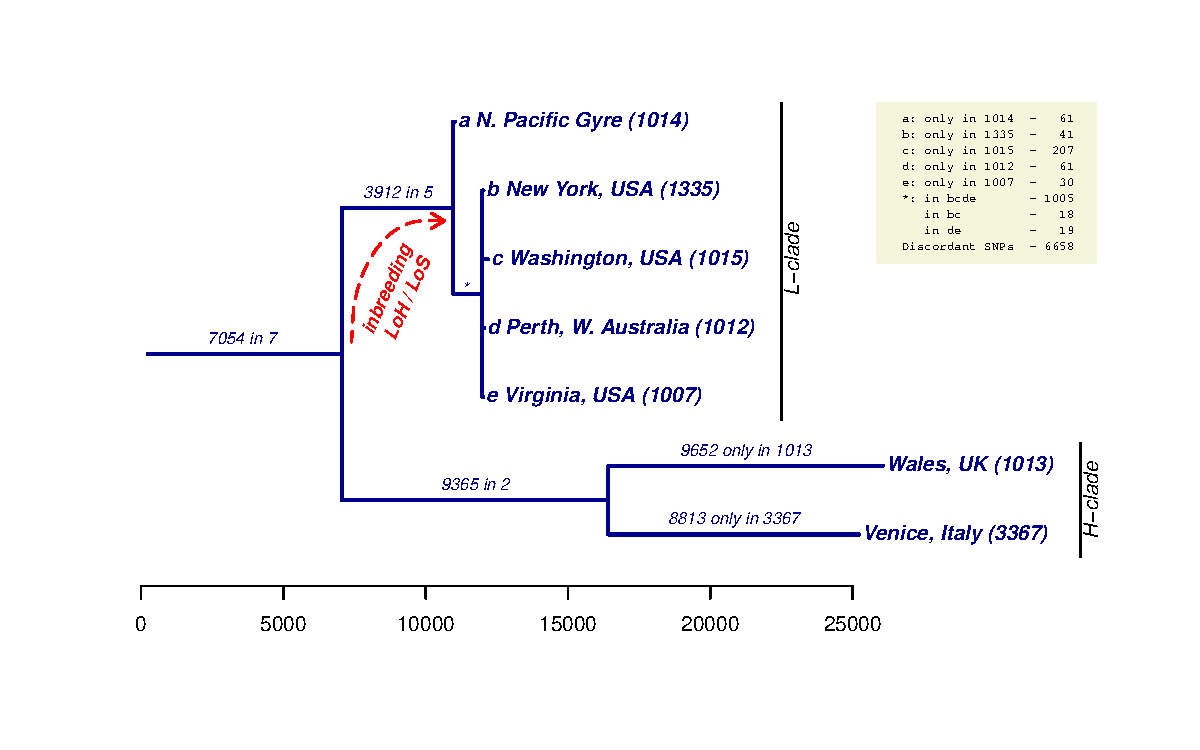
\includegraphics{figs-mine/paperfig-medium-tree-Chr1-unfiltered.pdf}
  \caption{Proposed fig. for paper: Tree based on unfiltered reads and medium SNP filters.  ``Lengths'' are numbers of shared/private SNPs on Chr1.}
  \label{fig:tree-paper}
\end{figure}

\begin{knitrout}\scriptsize
\definecolor{shadecolor}{rgb}{0.969, 0.969, 0.969}\color{fgcolor}\begin{kframe}
\begin{alltt}
\hlcom{# fig.paths for knitr chunks below;  .h for "hand-made" trees; plain for automatic chr1/full versions}
\hlstd{myfigpath}   \hlkwb{<-} \hlkwd{paste}\hlstd{(}\hlkwd{getwd}\hlstd{(),} \hlstr{'/figs-knitr/newick-'}\hlstd{,} \hlkwd{which.snp.tables}\hlstd{(),} \hlstr{'-'}\hlstd{,} \hlkwc{sep}\hlstd{=}\hlstr{''}\hlstd{)}
\hlstd{myfigpath.h} \hlkwb{<-} \hlkwd{paste}\hlstd{(}\hlkwd{getwd}\hlstd{(),} \hlstr{'/figs-knitr/newick-'}\hlstd{,} \hlkwc{sep}\hlstd{=}\hlstr{''}\hlstd{)}
\end{alltt}
\end{kframe}
\end{knitrout}

Figure~\ref{fig:tree-loose}, i.e., criteria [[1]]:

\begin{knitrout}\scriptsize
\definecolor{shadecolor}{rgb}{0.969, 0.969, 0.969}\color{fgcolor}\begin{kframe}
\begin{alltt}
\hlstd{newick.loose} \hlkwb{<-} \hlkwd{newickize}\hlstd{(}\hlkwd{make.tree}\hlstd{(pat.summaries[,}\hlstr{'count1'}\hlstd{]))}
\hlkwd{show.tree}\hlstd{(newick.loose,} \hlkwc{total.snps}\hlstd{=consistent.count[}\hlnum{1}\hlstd{])}
\end{alltt}
\end{kframe}\begin{figure}

{\centering 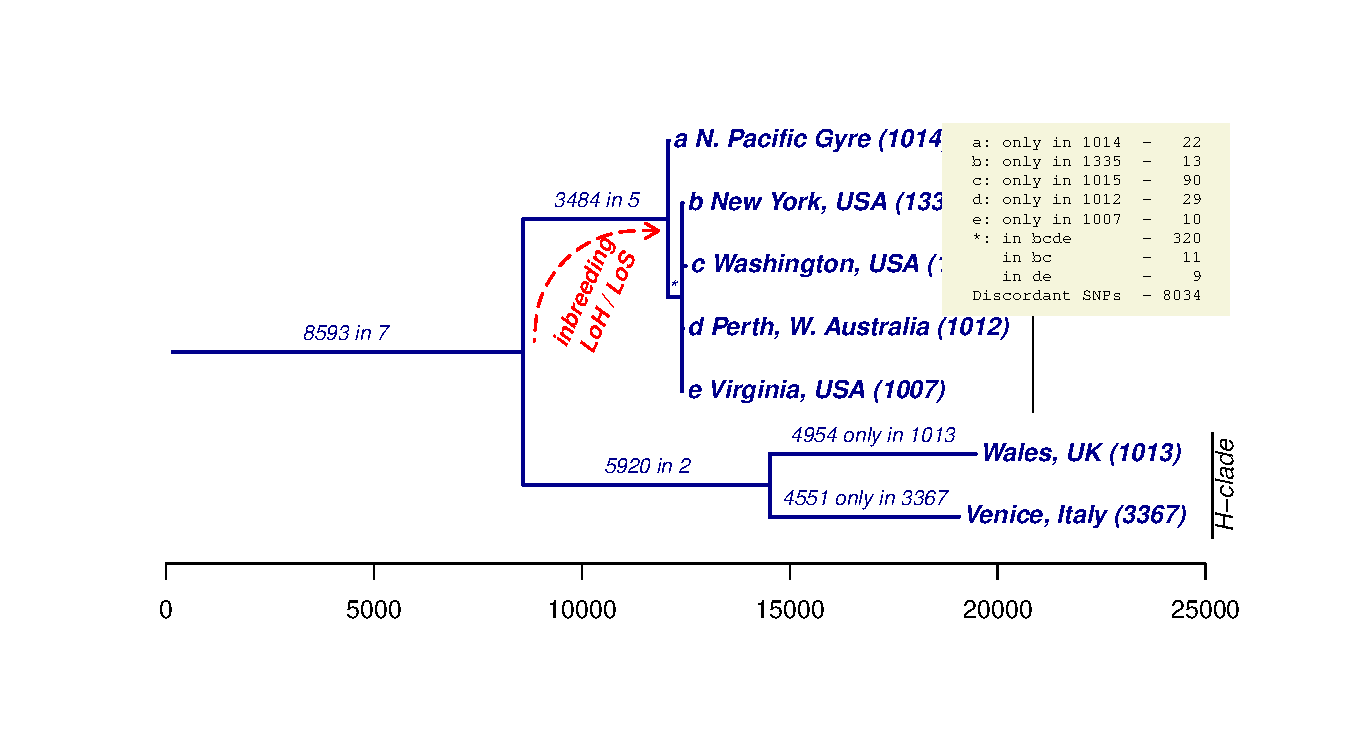
\includegraphics[width=\maxwidth]{/homes/gws/ruzzo/Documents/g/projects/thaps/Thaps_7_strains/code/snpNB/scripts/larrys/shared-snps/figs-knitr/newick-Chr1-unfiltered-tree-loose-1} 

}

\caption[Tree based on unfiltered reads and loose SNP filters]{Tree based on unfiltered reads and loose SNP filters.  ``Lengths'' are numbers of shared/private SNPs on Chr1.}\label{fig:tree-loose}
\end{figure}


\end{knitrout}

Figure~\ref{fig:tree-medium}, i.e. [[2]]:

\begin{knitrout}\scriptsize
\definecolor{shadecolor}{rgb}{0.969, 0.969, 0.969}\color{fgcolor}\begin{kframe}
\begin{alltt}
\hlcom{# newick.medium <- newickize(tree.by.hand)}
\hlcom{# simple.newick.medium <- newickize(tree.by.hand,alt=TRUE)}
\hlstd{newick.medium} \hlkwb{<-} \hlkwd{newickize}\hlstd{(}\hlkwd{make.tree}\hlstd{(pat.summaries[,}\hlstr{'count2'}\hlstd{]))}
\hlstd{simple.newick.medium} \hlkwb{<-} \hlkwd{newickize}\hlstd{(}\hlkwd{make.tree}\hlstd{(pat.summaries[,}\hlstr{'count2'}\hlstd{]),}\hlkwc{alt}\hlstd{=}\hlnum{TRUE}\hlstd{)}
\hlkwd{show.tree}\hlstd{(newick.medium,} \hlkwc{total.snps}\hlstd{=consistent.count[}\hlnum{2}\hlstd{])}
\end{alltt}
\end{kframe}\begin{figure}

{\centering 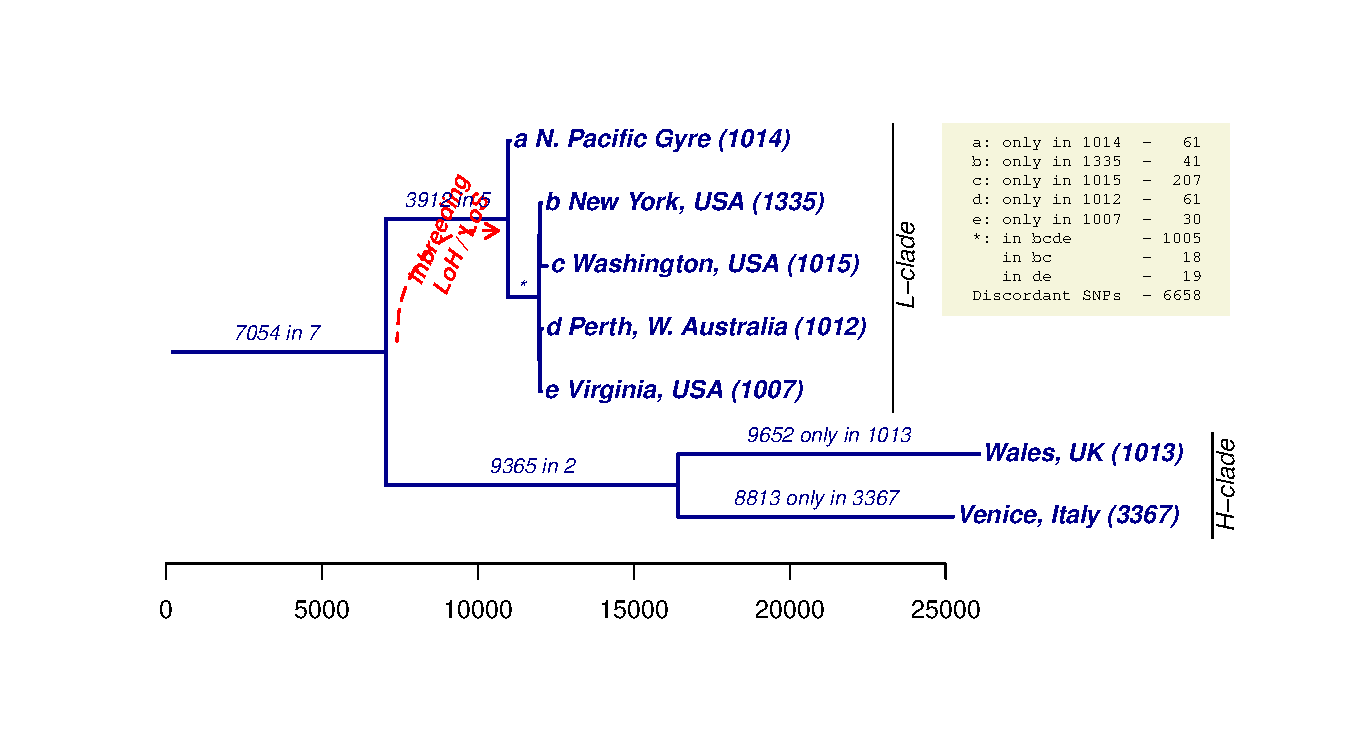
\includegraphics[width=\maxwidth]{/homes/gws/ruzzo/Documents/g/projects/thaps/Thaps_7_strains/code/snpNB/scripts/larrys/shared-snps/figs-knitr/newick-Chr1-unfiltered-tree-medium-1} 

}

\caption[Tree based on unfiltered reads and medium SNP filters]{Tree based on unfiltered reads and medium SNP filters.  ``Lengths'' are numbers of shared/private SNPs on Chr1.}\label{fig:tree-medium}
\end{figure}


\end{knitrout}

Figure~\ref{fig:tree-strict}, i.e. [[3]]:

\begin{knitrout}\scriptsize
\definecolor{shadecolor}{rgb}{0.969, 0.969, 0.969}\color{fgcolor}\begin{kframe}
\begin{alltt}
\hlstd{newick.strict} \hlkwb{<-} \hlkwd{newickize}\hlstd{(}\hlkwd{make.tree}\hlstd{(pat.summaries[,}\hlstr{'count3'}\hlstd{]))}
\hlkwd{show.tree}\hlstd{(newick.strict,} \hlkwc{total.snps}\hlstd{=consistent.count[}\hlnum{3}\hlstd{])}
\end{alltt}
\end{kframe}\begin{figure}

{\centering 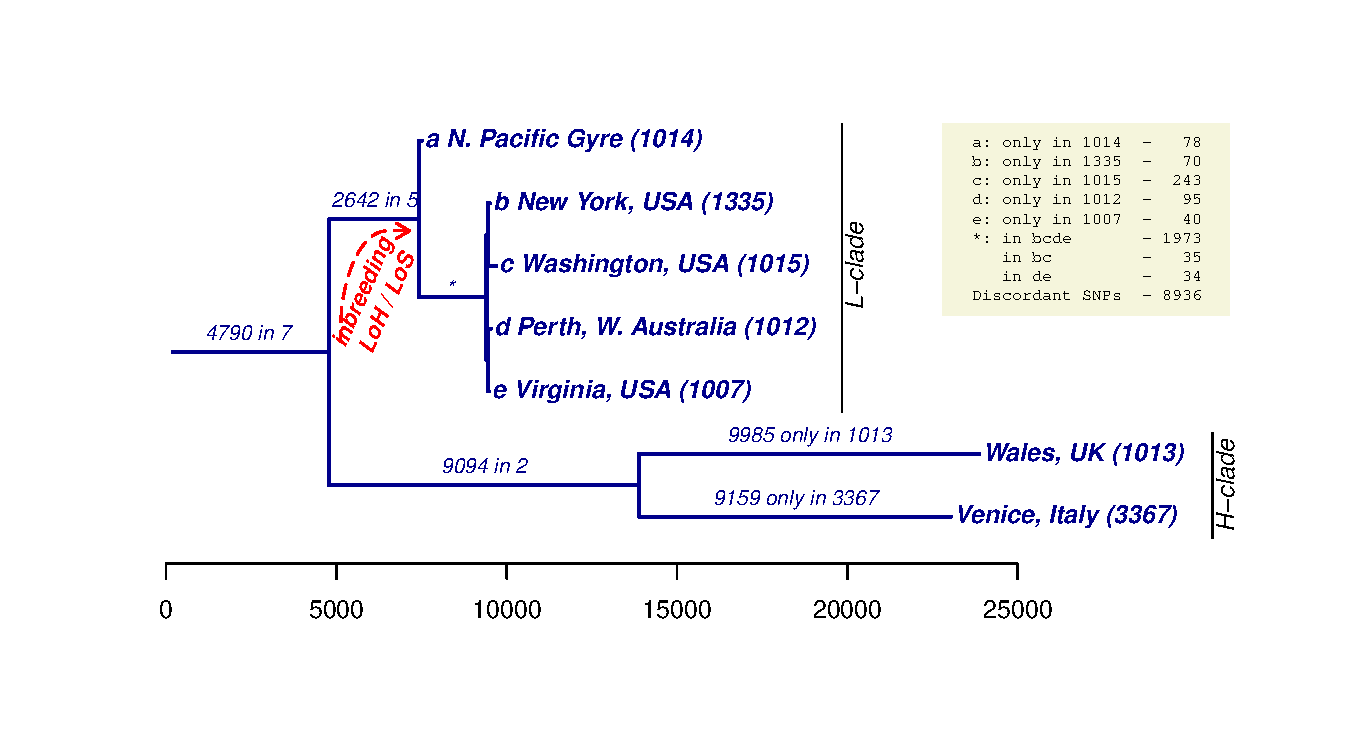
\includegraphics[width=\maxwidth]{/homes/gws/ruzzo/Documents/g/projects/thaps/Thaps_7_strains/code/snpNB/scripts/larrys/shared-snps/figs-knitr/newick-Chr1-unfiltered-tree-strict-1} 

}

\caption[Tree based on unfiltered reads and strict SNP filters]{Tree based on unfiltered reads and strict SNP filters.  ``Lengths'' are numbers of shared/private SNPs on Chr1.}\label{fig:tree-strict}
\end{figure}


\end{knitrout}

Figure~\ref{fig:tree-unfiltered}, i.e. [[4]]:

\begin{knitrout}\scriptsize
\definecolor{shadecolor}{rgb}{0.969, 0.969, 0.969}\color{fgcolor}\begin{kframe}
\begin{alltt}
\hlstd{newick.unfiltered} \hlkwb{<-} \hlkwd{newickize}\hlstd{(}\hlkwd{make.tree}\hlstd{(pat.summaries[,}\hlstr{'count4'}\hlstd{]))}
\hlkwd{show.tree}\hlstd{(newick.unfiltered,} \hlkwc{total.snps}\hlstd{=consistent.count[}\hlnum{4}\hlstd{])}
\end{alltt}
\end{kframe}\begin{figure}

{\centering 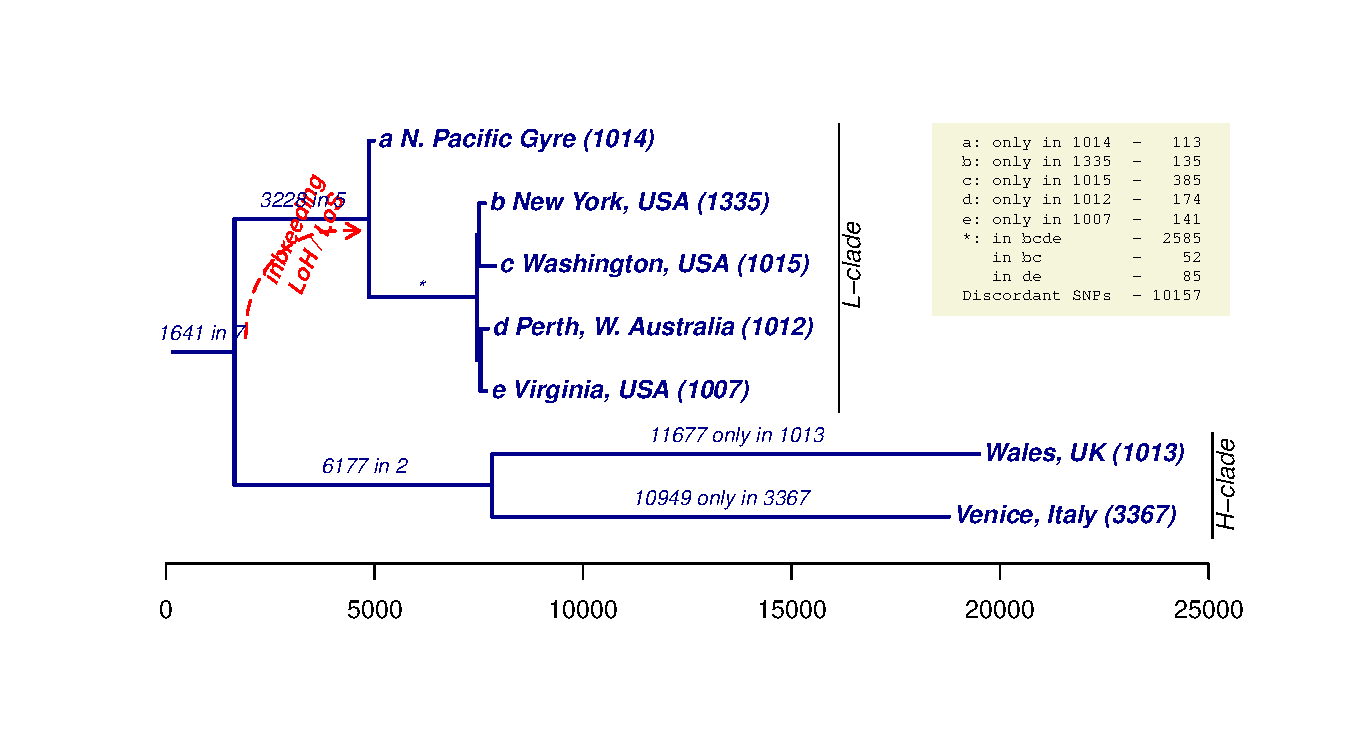
\includegraphics[width=\maxwidth]{/homes/gws/ruzzo/Documents/g/projects/thaps/Thaps_7_strains/code/snpNB/scripts/larrys/shared-snps/figs-knitr/newick-Chr1-unfiltered-tree-unfiltered-1} 

}

\caption[Tree based on unfiltered reads and unfiltered SNPs]{Tree based on unfiltered reads and unfiltered SNPs.  ``Lengths'' are numbers of shared/private SNPs on Chr1.}\label{fig:tree-unfiltered}
\end{figure}


\end{knitrout}

Some other versions of the trees are included in the appendix.

Counts for all tree edges in the medium tree: 

\begin{knitrout}\scriptsize
\definecolor{shadecolor}{rgb}{0.969, 0.969, 0.969}\color{fgcolor}\begin{kframe}
\begin{alltt}
\hlcom{#pat.summaries[c(128,110,102,6,97,19,9,2,5,33,65,17,3),]}
\hlstd{tree.edges} \hlkwb{<-} \hlkwd{c}\hlstd{(}\hlnum{128}\hlstd{,}\hlnum{110}\hlstd{,}\hlnum{102}\hlstd{,}\hlnum{6}\hlstd{,}\hlnum{97}\hlstd{,}\hlnum{19}\hlstd{,}\hlnum{9}\hlstd{,}\hlnum{2}\hlstd{,}\hlnum{5}\hlstd{,}\hlnum{33}\hlstd{,}\hlnum{65}\hlstd{,}\hlnum{17}\hlstd{,}\hlnum{3}\hlstd{)}\hlopt{-}\hlnum{1}
\hlstd{non.edges} \hlkwb{<-} \hlkwd{setdiff}\hlstd{(}\hlnum{0}\hlopt{:}\hlnum{127}\hlstd{, tree.edges)}
\hlstd{sg.edges} \hlkwb{<-} \hlkwd{showgroup}\hlstd{(}\hlkwc{restrict.to}\hlstd{=tree.edges) ; sg.edges}
\end{alltt}
\begin{verbatim}
#       Pat ShrBy 1007 1012 1013 1014 1015 3367 1335 count1 count2 count3 count4
# 2     001     1                                  X     13     41     70    135
# 3     002     1                             X        4551   8813   9159  10949
# 5     004     1                        X               90    207    243    385
# 6     005     2                        X         X     11     18     35     52
# 9     010     1                   X                    22     61     78    113
# 17    020     1              X                       4954   9652   9985  11677
# 19    022     2              X              X        5920   9365   9094   6177
# 33    040     1         X                              29     61     95    174
# 65    100     1    X                                   10     30     40    141
# 97    140     2    X    X                               9     19     34     85
# 102   145     4    X    X              X         X    320   1005   1973   2585
# 110   155     5    X    X         X    X         X   3484   3912   2642   3228
# 128   177     7    X    X    X    X    X    X    X   8593   7054   4790   1641
# Total                                               28006  40238  38238  37342
\end{verbatim}
\end{kframe}
\end{knitrout}

Counts for the top 10 discordant patterns, i.e., SNPs whose sharing pattern does not match any of the bifurcations in the tree:

\begin{knitrout}\scriptsize
\definecolor{shadecolor}{rgb}{0.969, 0.969, 0.969}\color{fgcolor}\begin{kframe}
\begin{alltt}
\hlstd{tenth} \hlkwb{<-} \hlkwd{sort}\hlstd{(}\hlkwd{showgroup}\hlstd{(}\hlkwc{restrict.to}\hlstd{=non.edges)[}\hlopt{-}\hlstd{(}\hlkwd{length}\hlstd{(non.edges)}\hlopt{+}\hlnum{1}\hlstd{),}\hlstr{'count2'}\hlstd{],}\hlkwc{decreasing}\hlstd{=T)[}\hlnum{10}\hlstd{]}
\hlstd{sg.non.edges} \hlkwb{<-} \hlkwd{showgroup}\hlstd{(}\hlkwc{restrict.to}\hlstd{=non.edges,} \hlkwc{c2.thresh} \hlstd{= tenth) ; sg.non.edges}
\end{alltt}
\begin{verbatim}
#       Pat ShrBy 1007 1012 1013 1014 1015 3367 1335 count1 count2 count3 count4
# 56    067     5         X    X         X    X    X     33     78    201    104
# 101   144     3    X    X              X                6     75    167    355
# 104   147     5    X    X              X    X    X    125    307    590   1160
# 109   154     4    X    X         X    X               16     53     49    103
# 112   157     6    X    X         X    X    X    X   1343   1192    839   1343
# 118   165     5    X    X    X         X         X    201    453    787   1140
# 119   166     5    X    X    X         X    X          30    157    247    254
# 120   167     6    X    X    X         X    X    X    951   1879   3320   1852
# 126   175     6    X    X    X    X    X         X   1756   1493    997   1416
# 127   176     6    X    X    X    X    X    X          45    114     77     68
# Other   (   105 rows   w/   c2    <   53    )        3528    857   1662   2362
# Total                                                8034   6658   8936  10157
\end{verbatim}
\end{kframe}
\end{knitrout}

And percent of discordant SNPs:

\begin{knitrout}\scriptsize
\definecolor{shadecolor}{rgb}{0.969, 0.969, 0.969}\color{fgcolor}\begin{kframe}
\begin{alltt}
\hlstd{nsge} \hlkwb{<-} \hlkwd{nrow}\hlstd{(sg.edges)}
\hlstd{discordv} \hlkwb{<-} \hlstd{consistent.count} \hlopt{-} \hlstd{sg.edges[nsge,}\hlkwd{c}\hlstd{(}\hlstr{'count1'}\hlstd{,}\hlstr{'count2'}\hlstd{,}\hlstr{'count3'}\hlstd{,}\hlstr{'count4'}\hlstd{)] ; discordv}
\end{alltt}
\begin{verbatim}
#       count1 count2 count3 count4
# Total   8034   6658   8936  10157
\end{verbatim}
\begin{alltt}
\hlstd{discordv.pct} \hlkwb{<-} \hlkwd{round}\hlstd{(discordv}\hlopt{/}\hlstd{consistent.count}\hlopt{*}\hlnum{100}\hlstd{,}\hlnum{1}\hlstd{) ; discordv.pct}
\end{alltt}
\begin{verbatim}
#       count1 count2 count3 count4
# Total   22.3   14.2   18.9   21.4
\end{verbatim}
\end{kframe}
\end{knitrout}

In short, the sharing pattern observed at 6658 or 14.2\% of the 
46896 medium-stringency consistent SNPs positions observed across all 7 
isolates are discordant with the medium tree.  (The strict tree has slightly more.)  

A majority of the discordant SNPs fall into one of three patterns: 6-way sharing excluding Gyre 
(likely a technical artifact since the low coverage in Gyre reduces our power to detect SNPs there), 
or 6-way sharing excluding one of the two H-isolates (likely a reflection of sexuality in the 
H-clade---SNP positions in a population in Hardy-Weinberg equilibrium are fairly likely to be 
homozygous for the reference allele in a given individual).

\begin{knitrout}\scriptsize
\definecolor{shadecolor}{rgb}{0.969, 0.969, 0.969}\color{fgcolor}\begin{kframe}
\begin{alltt}
\hlstd{third.biggest} \hlkwb{<-} \hlkwd{sort}\hlstd{(}\hlkwd{showgroup}\hlstd{(pat.summaries,}\hlnum{6}\hlstd{)[}\hlopt{-}\hlnum{8}\hlstd{,}\hlstr{'count2'}\hlstd{],}\hlkwc{decreasing}\hlstd{=T)[}\hlnum{3}\hlstd{]}
\hlstd{big.three} \hlkwb{<-} \hlkwd{showgroup}\hlstd{(pat.summaries,}\hlnum{6}\hlstd{,}\hlkwc{c2.thresh} \hlstd{= third.biggest); big.three}
\end{alltt}
\begin{verbatim}
#       Pat ShrBy 1007 1012 1013 1014 1015 3367 1335 count1 count2 count3 count4
# 112   157     6    X    X         X    X    X    X   1343   1192    839   1343
# 120   167     6    X    X    X         X    X    X    951   1879   3320   1852
# 126   175     6    X    X    X    X    X         X   1756   1493    997   1416
# Other   (     4 rows   w/   c2    < 1192    )         116    177    156    111
# Total                                                4166   4741   5312   4722
\end{verbatim}
\begin{alltt}
\hlstd{big.three.frac} \hlkwb{<-} \hlkwd{sum}\hlstd{(big.three[}\hlnum{1}\hlopt{:}\hlnum{3}\hlstd{,}\hlstr{'count2'}\hlstd{])}\hlopt{/}\hlstd{discordv}\hlopt{$}\hlstd{count2; big.three.frac}
\end{alltt}
\begin{verbatim}
# [1] 0.6854911
\end{verbatim}
\end{kframe}
\end{knitrout}

\noindent I.e., 68.5\% of discordant SNPs fall into one of these three 
categories.

Out of curiousity: what is the ratio of full genome to Chr 1 branch lengths.  Except for the shortest 
few, generally $\approx$10x, as expected given the length of Chr 1:

\begin{knitrout}\scriptsize
\definecolor{shadecolor}{rgb}{0.969, 0.969, 0.969}\color{fgcolor}\begin{kframe}
\begin{alltt}
\hlcom{# (vectors derived by editing Newick strings, and in that order)}
\hlkwd{print}\hlstd{(}
  \hlkwd{c}\hlstd{(}\hlkwc{Italy}\hlstd{=}\hlnum{86155}\hlstd{,} \hlkwc{Wales}\hlstd{=}\hlnum{95697}\hlstd{,} \hlkwc{IW}\hlstd{=}\hlnum{89598}\hlstd{,} \hlkwc{Virg}\hlstd{=}\hlnum{330}\hlstd{,}     \hlkwc{Aust}\hlstd{=}\hlnum{632}\hlstd{,}      \hlkwc{VA}\hlstd{=}\hlnum{1296}\hlstd{,}
    \hlkwc{Puget}\hlstd{=}\hlnum{2113}\hlstd{,}  \hlkwc{NY}\hlstd{=}\hlnum{658}\hlstd{,}      \hlkwc{PNY}\hlstd{=}\hlnum{480}\hlstd{,}  \hlkwc{four}\hlstd{=}\hlnum{10059}\hlstd{,}   \hlkwc{Gyre}\hlstd{=}\hlnum{568}\hlstd{,}      \hlkwc{five}\hlstd{=}\hlnum{39517}\hlstd{,} \hlkwc{all}\hlstd{=}\hlnum{69526}\hlstd{)} \hlopt{/}
  \hlkwd{c}\hlstd{(}\hlkwc{Italy}\hlstd{=}\hlnum{8813}\hlstd{,}  \hlkwc{Wales}\hlstd{=}\hlnum{9652}\hlstd{,}  \hlkwc{IW}\hlstd{=}\hlnum{9365}\hlstd{,}  \hlkwc{Virg}\hlstd{=}\hlnum{30}\hlstd{,}      \hlkwc{Aust}\hlstd{=}\hlnum{61}\hlstd{,}       \hlkwc{VA}\hlstd{=}\hlnum{19}\hlstd{,}
    \hlkwc{Puget}\hlstd{=}\hlnum{207}\hlstd{,}   \hlkwc{NY}\hlstd{=}\hlnum{41}\hlstd{,}       \hlkwc{PNY}\hlstd{=}\hlnum{18}\hlstd{,}   \hlkwc{four}\hlstd{=}\hlnum{1005}\hlstd{,}    \hlkwc{Gyre}\hlstd{=}\hlnum{61}\hlstd{,}       \hlkwc{five}\hlstd{=}\hlnum{3912}\hlstd{,}  \hlkwc{all}\hlstd{=} \hlnum{7054}\hlstd{),}
  \hlkwc{digits}\hlstd{=}\hlnum{3}\hlstd{)}
\end{alltt}
\begin{verbatim}
# Italy Wales    IW  Virg  Aust    VA Puget    NY   PNY  four  Gyre  five   all 
#  9.78  9.91  9.57 11.00 10.36 68.21 10.21 16.05 26.67 10.01  9.31 10.10  9.86
\end{verbatim}
\begin{alltt}
\hlkwd{round}\hlstd{(}\hlkwd{genome.length.constants}\hlstd{()}\hlopt{$}\hlstd{genome.length.trunc} \hlopt{/} \hlkwd{genome.length.constants}\hlstd{()}\hlopt{$}\hlstd{chr1.length,} \hlkwc{digits}\hlstd{=}\hlnum{4}\hlstd{)}
\end{alltt}
\begin{verbatim}
# [1] 10.2879
\end{verbatim}
\end{kframe}
\end{knitrout}

\section{Semi-Automated Tree-Building}
Slightly formalizing the process above: Look for the bifurcation of the 7 strains that maximizes the 
number of shared SNPs \emph{within} each side of the partition while minimizing the number and 
fraction of SNPs that are shared by subsets that include at least one strain on each side of the 
partition.  The 2/5 split is the winner, with 6418 SNPs in confict with that partition (16\% of the 
39842 SNPs not shared by all 7; Chr1 data).  The runner-up places the Gyre in a group by
itself (7079 = 18\% in conflict).

\begin{knitrout}\footnotesize
\definecolor{shadecolor}{rgb}{0.969, 0.969, 0.969}\color{fgcolor}\begin{kframe}
\begin{alltt}
\hlstd{treepart} \hlkwb{<-} \hlkwa{function}\hlstd{(}\hlkwc{p.summ}\hlstd{=pat.summaries,} \hlkwc{root}\hlstd{=}\hlnum{127}\hlstd{,} \hlkwc{verbose}\hlstd{=T,} \hlkwc{stringency}\hlstd{=}\hlstr{'count2'}\hlstd{)\{}
  \hlstd{root.shared} \hlkwb{<-} \hlstd{p.summ[root}\hlopt{+}\hlnum{1}\hlstd{,stringency]}
  \hlstd{df}\hlkwb{<-}\hlkwa{NULL}
  \hlkwa{for}\hlstd{(i} \hlkwa{in} \hlnum{1}\hlopt{:}\hlkwd{floor}\hlstd{(root}\hlopt{/}\hlnum{2}\hlstd{))\{}
    \hlkwa{if}\hlstd{(}\hlkwd{bitwAnd}\hlstd{(i,root)}\hlopt{==}\hlstd{i} \hlopt{&&} \hlstd{i} \hlopt{<} \hlstd{root}\hlopt{-}\hlstd{i)\{}
      \hlstd{l1} \hlkwb{<-} \hlkwd{showgroup}\hlstd{(p.summ,}\hlkwc{subset}\hlstd{=i,}\hlkwc{split}\hlstd{=}\hlkwa{NULL}\hlstd{,}\hlkwc{proper.subset}\hlstd{=F,}\hlkwc{total}\hlstd{=T)}
      \hlstd{l}  \hlkwb{<-} \hlstd{l1[}\hlkwd{nrow}\hlstd{(l1),stringency]}
      \hlstd{r1} \hlkwb{<-} \hlkwd{showgroup}\hlstd{(p.summ,}\hlkwc{subset}\hlstd{=root}\hlopt{-}\hlstd{i,}\hlkwc{split}\hlstd{=}\hlkwa{NULL}\hlstd{,}\hlkwc{proper.subset}\hlstd{=F,}\hlkwc{total}\hlstd{=T)}
      \hlstd{r}  \hlkwb{<-} \hlstd{r1[}\hlkwd{nrow}\hlstd{(r1),stringency]}
      \hlstd{c1} \hlkwb{<-} \hlkwd{showgroup}\hlstd{(p.summ,}\hlkwc{subset}\hlstd{=root,}\hlkwc{split}\hlstd{=i,}\hlkwc{proper.subset}\hlstd{=T,}\hlkwc{total}\hlstd{=T)}
      \hlstd{c}  \hlkwb{<-} \hlstd{c1[}\hlkwd{nrow}\hlstd{(c1),stringency]}
      \hlstd{df} \hlkwb{<-} \hlkwd{rbind}\hlstd{(df,} \hlkwd{data.frame}\hlstd{(}\hlkwc{pat}\hlstd{=i,}\hlkwc{left}\hlstd{=l,}\hlkwc{right}\hlstd{=r,}\hlkwc{both}\hlstd{=l}\hlopt{+}\hlstd{r,}\hlkwc{cross}\hlstd{=c,}\hlkwc{all}\hlstd{=l}\hlopt{+}\hlstd{r}\hlopt{+}\hlstd{c,}\hlkwc{ratio}\hlstd{=c}\hlopt{/}\hlstd{(l}\hlopt{+}\hlstd{r}\hlopt{+}\hlstd{c),}
                                 \hlkwc{best}\hlstd{=}\hlstr{''}\hlstd{,}\hlkwc{stringsAsFactors}\hlstd{=F))}
    \hlstd{\}}
  \hlstd{\}}
  \hlstd{df}\hlopt{$}\hlstd{pat}\hlkwb{<-}\hlkwd{as.octmode}\hlstd{(df}\hlopt{$}\hlstd{pat)}
  \hlstd{maxl} \hlkwb{<-} \hlkwd{which.max}\hlstd{(df}\hlopt{$}\hlstd{left)}
  \hlstd{maxr} \hlkwb{<-} \hlkwd{which.max}\hlstd{(df}\hlopt{$}\hlstd{right)}
  \hlstd{maxb} \hlkwb{<-} \hlkwd{which.max}\hlstd{(df}\hlopt{$}\hlstd{both)}
  \hlstd{minc} \hlkwb{<-} \hlkwd{which.min}\hlstd{(df}\hlopt{$}\hlstd{cross)}
  \hlstd{minr} \hlkwb{<-} \hlkwd{which.min}\hlstd{(df}\hlopt{$}\hlstd{ratio)}
  \hlstd{df}\hlopt{$}\hlstd{best[}\hlkwd{c}\hlstd{(maxl,maxr,maxb,minc,minr)]} \hlkwb{<-} \hlstr{'<'}
  \hlstd{df}\hlopt{$}\hlstd{best[maxl]} \hlkwb{<-} \hlkwd{paste}\hlstd{(df}\hlopt{$}\hlstd{best[maxl],} \hlstr{'L'}\hlstd{)} \hlcom{# max Left}
  \hlstd{df}\hlopt{$}\hlstd{best[maxr]} \hlkwb{<-} \hlkwd{paste}\hlstd{(df}\hlopt{$}\hlstd{best[maxr],} \hlstr{'R'}\hlstd{)} \hlcom{# max Right}
  \hlstd{df}\hlopt{$}\hlstd{best[maxb]} \hlkwb{<-} \hlkwd{paste}\hlstd{(df}\hlopt{$}\hlstd{best[maxb],} \hlstr{'B'}\hlstd{)} \hlcom{# max Both (L+R)}
  \hlstd{df}\hlopt{$}\hlstd{best[minc]} \hlkwb{<-} \hlkwd{paste}\hlstd{(df}\hlopt{$}\hlstd{best[minc],} \hlstr{'C'}\hlstd{)} \hlcom{# min Cross}
  \hlstd{df}\hlopt{$}\hlstd{best[minr]} \hlkwb{<-} \hlkwd{paste}\hlstd{(df}\hlopt{$}\hlstd{best[minr],} \hlstr{'O'}\hlstd{)} \hlcom{# min ratiO (Cross/(Left+Right+Cross)}
  \hlkwa{if}\hlstd{(verbose)\{}
    \hlstd{same} \hlkwb{<-} \hlkwd{all}\hlstd{(maxl}\hlopt{==}\hlkwd{c}\hlstd{(maxr,maxb,minc,minr))}
    \hlkwd{cat}\hlstd{(}\hlstr{'root:'}\hlstd{,}       \hlkwd{format}\hlstd{(}\hlkwd{as.octmode}\hlstd{(root),}\hlkwc{width}\hlstd{=}\hlnum{3}\hlstd{),}
        \hlstr{'; shared:'}\hlstd{,   root.shared,}
        \hlstr{'.  max l'}\hlstd{,}    \hlkwd{format}\hlstd{(}\hlkwd{as.octmode}\hlstd{(df}\hlopt{$}\hlstd{pat[maxl]),}\hlkwc{width}\hlstd{=}\hlnum{3}\hlstd{),}
        \hlstr{', max r'}\hlstd{,}     \hlkwd{format}\hlstd{(}\hlkwd{as.octmode}\hlstd{(df}\hlopt{$}\hlstd{pat[maxr]),}\hlkwc{width}\hlstd{=}\hlnum{3}\hlstd{),}
        \hlstr{', max both'}\hlstd{,}  \hlkwd{format}\hlstd{(}\hlkwd{as.octmode}\hlstd{(df}\hlopt{$}\hlstd{pat[maxb]),}\hlkwc{width}\hlstd{=}\hlnum{3}\hlstd{),}
        \hlstr{', min cross'}\hlstd{,} \hlkwd{format}\hlstd{(}\hlkwd{as.octmode}\hlstd{(df}\hlopt{$}\hlstd{pat[minc]),}\hlkwc{width}\hlstd{=}\hlnum{3}\hlstd{),}
        \hlstr{', min ratio'}\hlstd{,} \hlkwd{format}\hlstd{(}\hlkwd{as.octmode}\hlstd{(df}\hlopt{$}\hlstd{pat[minr]),}\hlkwc{width}\hlstd{=}\hlnum{3}\hlstd{),}
        \hlstr{'. \textbackslash{}nAll the same?:'}\hlstd{,same,}
        \hlstr{'\textbackslash{}n'}\hlstd{)}
    \hlkwd{cat}\hlstd{(}\hlstr{'\textbackslash{}n'}\hlstd{)}
  \hlstd{\}}
  \hlkwd{return}\hlstd{(df)}
\hlstd{\}}
\end{alltt}
\end{kframe}
\end{knitrout}

\begin{knitrout}\footnotesize
\definecolor{shadecolor}{rgb}{0.969, 0.969, 0.969}\color{fgcolor}\begin{kframe}
\begin{alltt}
\hlkwd{treepart}\hlstd{()}
\end{alltt}
\begin{verbatim}
# root: 177 ; shared: 7054 .  max l 077 , max r 010 , max both 022 , min cross 022 , min ratio 022 . 
# All the same?: FALSE
#    pat  left right  both cross   all     ratio    best
# 1   01    41 29077 29118 10724 39842 0.2691632        
# 2   02  8813 17400 26213 13629 39842 0.3420762        
# 3   03  8870 10338 19208 20634 39842 0.5178957        
# 4   04   207 28345 28552 11290 39842 0.2833693        
# 5   05   266 28142 28408 11434 39842 0.2869836        
# 6   06  9033  9956 18989 20853 39842 0.5233924        
# 7   07  9110  9866 18976 20866 39842 0.5237187        
# 8   10    61 32702 32763  7079 39842 0.1776768     < R
# 9   11   109 28694 28803 11039 39842 0.2770694        
# 10  12  8892 11759 20651 19191 39842 0.4816776        
# 11  13  8959 10160 19119 20723 39842 0.5201295        
# 12  14   270 28163 28433 11409 39842 0.2863561        
# 13  15   342 28006 28348 11494 39842 0.2884895        
# 14  16  9115  9849 18964 20878 39842 0.5240199        
# 15  17  9213  9781 18994 20848 39842 0.5232669        
# 16  20  9652 16099 25751 14091 39842 0.3536720        
# 17  21  9702  9470 19172 20670 39842 0.5187993        
# 18  22 27830  5594 33424  6418 39842 0.1610863 < B C O
# 19  23 27916   542 28458 11384 39842 0.2857286        
# 20  24  9871  9119 18990 20852 39842 0.5233673        
# 21  25  9943  9016 18959 20883 39842 0.5241454        
# 22  26 28089   239 28328 11514 39842 0.2889915        
# 23  27 28213   175 28388 11454 39842 0.2874856        
# 24  30  9731 10772 20503 19339 39842 0.4853923        
# 25  31  9790  9303 19093 20749 39842 0.5207821        
# 26  32 27945  1520 29465 10377 39842 0.2604538        
# 27  33 28045   414 28459 11383 39842 0.2857035        
# 28  34  9955  9014 18969 20873 39842 0.5238944        
# 29  35 10044  8931 18975 20867 39842 0.5237438        
# 30  36 28214   162 28376 11466 39842 0.2877868        
# 31  37 28375   110 28485 11357 39842 0.2850510        
# 32  40    61 28554 28615 11227 39842 0.2817881        
# 33  41   106 28330 28436 11406 39842 0.2862808        
# 34  42  8875 10122 18997 20845 39842 0.5231916        
# 35  43  8944 10017 18961 20881 39842 0.5240952        
# 36  44   281 28125 28406 11436 39842 0.2870338        
# 37  45   370 28005 28375 11467 39842 0.2878119        
# 38  46  9120  9835 18955 20887 39842 0.5242458        
# 39  47  9253  9773 19026 20816 39842 0.5224637        
# 40  50   124 28358 28482 11360 39842 0.2851262        
# 41  51   177 28189 28366 11476 39842 0.2880377        
# 42  52  8956 10008 18964 20878 39842 0.5240199        
# 43  53  9036  9926 18962 20880 39842 0.5240701        
# 44  54   352 27986 28338 11504 39842 0.2887405        
# 45  55   467 27885 28352 11490 39842 0.2883891        
# 46  56  9212  9743 18955 20887 39842 0.5242458        
# 47  57  9386  9691 19077 20765 39842 0.5211837        
# 48  60  9717  9297 19014 20828 39842 0.5227649        
# 49  61  9773  9175 18948 20894 39842 0.5244215        
# 50  62 27913   396 28309 11533 39842 0.2894684        
# 51  63 28024   313 28337 11505 39842 0.2887656        
# 52  64  9958  9006 18964 20878 39842 0.5240199        
# 53  65 10079  8931 19010 20832 39842 0.5228653        
# 54  66 28243   143 28386 11456 39842 0.2875358        
# 55  67 28531    93 28624 11218 39842 0.2815622        
# 56  70  9799  9180 18979 20863 39842 0.5236434        
# 57  71  9866  9087 18953 20889 39842 0.5242960        
# 58  72 28037   312 28349 11493 39842 0.2884644        
# 59  73 28167   246 28413 11429 39842 0.2868581        
# 60  74 10054  8912 18966 20876 39842 0.5239697        
# 61  75 10217  8849 19066 20776 39842 0.5214598        
# 62  76 28399    73 28472 11370 39842 0.2853772        
# 63  77 28807    30 28837 11005 39842 0.2762161     < L
\end{verbatim}
\end{kframe}
\end{knitrout}

Comparing the 5/2 split to the second-place NPG/rest split (below), the former has fewer pattern instances in conflict
with the split (6418 vs 7079), as well as somewhat more random distribution of the conflicting patterns (92 vs 62 rows),
whereas the 1/6 split has the majority of its conflicts (3912 of 7079, or 55\%) concentrated in one pattern---the 5 NE
strains.  Collectively, these seem to favor the 5/2 split as the correct ``history.''

\begin{knitrout}\footnotesize
\definecolor{shadecolor}{rgb}{0.969, 0.969, 0.969}\color{fgcolor}\begin{kframe}
\begin{alltt}
\hlkwd{showgroup}\hlstd{(pat.summaries,}\hlkwc{split}\hlstd{=}\hlkwd{strtoi}\hlstd{(}\hlstr{'022'}\hlstd{),} \hlkwc{subset}\hlstd{=}\hlnum{127}\hlstd{,} \hlkwc{proper.subset}\hlstd{=T,} \hlkwc{c2.thresh}\hlstd{=}\hlnum{100}\hlstd{)}
\end{alltt}
\begin{verbatim}
#       Pat ShrBy 1007 1012 1013 1014 1015 3367 1335 count1 count2 count3 count4
# 104   147     5    X    X              X    X    X    125    307    590   1160
# 112   157     6    X    X         X    X    X    X   1343   1192    839   1343
# 118   165     5    X    X    X         X         X    201    453    787   1140
# 119   166     5    X    X    X         X    X          30    157    247    254
# 120   167     6    X    X    X         X    X    X    951   1879   3320   1852
# 126   175     6    X    X    X    X    X         X   1756   1493    997   1416
# 127   176     6    X    X    X    X    X    X          45    114     77     68
# Other   (    85 rows   w/   c2    <  100    )        3493    823   1387   1771
# Total                                                7944   6418   8244   9004
\end{verbatim}
\begin{alltt}
\hlkwd{showgroup}\hlstd{(pat.summaries,}\hlkwc{split}\hlstd{=}\hlkwd{strtoi}\hlstd{(}\hlstr{'010'}\hlstd{),} \hlkwc{subset}\hlstd{=}\hlnum{127}\hlstd{,} \hlkwc{proper.subset}\hlstd{=T,} \hlkwc{c2.thresh}\hlstd{=}\hlnum{100}\hlstd{)}
\end{alltt}
\begin{verbatim}
#       Pat ShrBy 1007 1012 1013 1014 1015 3367 1335 count1 count2 count3 count4
# 110   155     5    X    X         X    X         X   3484   3912   2642   3228
# 112   157     6    X    X         X    X    X    X   1343   1192    839   1343
# 126   175     6    X    X    X    X    X         X   1756   1493    997   1416
# 127   176     6    X    X    X    X    X    X          45    114     77     68
# Other   (    58 rows   w/   c2    <  100    )        1095    368    368    522
# Total                                                7723   7079   4923   6577
\end{verbatim}
\end{kframe}
\end{knitrout}

Below is the full summary of shared SNPs that do \emph{not} directly correspond to tree splits, e.g. deep coalescence, independent coincident mutations, false positives/false negatives in the shared SNP calls, loss of SNPs in hemizygous regions, etc.  (Additionally, SAMTools' SNP calls exclude positions it judges to be homozygous, and I think it operates without regard to the reference sequence, so homozygous nonreference positions, while rare except in IT/Wales, often are not called SNPs by SAMTools, but are relevant for this analysis.  Provided the position is called a SNP in some other isolate, the consistency filtering we've done above should recover it, but this is still worth keeping in mind when examining the data.) 

First, here are SNPs that ``coalesce'' on the branch from the LCA of bcde, i.e., shared among some nonempty, proper subset of bcde other than bc or de.  There are 8 such patterns: any of the 4 choose 3 trios plus any of the 4 pairs having exactly one of bc. 

\begin{knitrout}\footnotesize
\definecolor{shadecolor}{rgb}{0.969, 0.969, 0.969}\color{fgcolor}\begin{kframe}
\begin{alltt}
\hlstd{sg4} \hlkwb{<-} \hlkwd{showgroup}\hlstd{(pat.summaries,} \hlkwc{subset}\hlstd{=}\hlkwd{strtoi}\hlstd{(}\hlstr{'0145'}\hlstd{),} \hlkwc{split}\hlstd{=}\hlnum{5}\hlstd{,} \hlkwc{proper.subset} \hlstd{= F)}
\hlstd{sg4}
\end{alltt}
\begin{verbatim}
#       Pat ShrBy 1007 1012 1013 1014 1015 3367 1335 count1 count2 count3 count4
# 34    041     2         X                        X      3      4     13     36
# 37    044     2         X              X                5     13     75    155
# 38    045     3         X              X         X      6     26    130    131
# 66    101     2    X                             X      1      2     13     20
# 69    104     2    X                   X                5      9     34    107
# 70    105     3    X                   X         X      4      5     25     63
# 98    141     3    X    X                        X      2      5     15     40
# 101   144     3    X    X              X                6     75    167    355
# 102   145     4    X    X              X         X    320   1005   1973   2585
# Total                                                 352   1144   2445   3492
\end{verbatim}
\begin{alltt}
\hlstd{sg4n} \hlkwb{<-} \hlkwd{nrow}\hlstd{(sg4)}
\hlstd{sg4pct} \hlkwb{<-} \hlkwd{round}\hlstd{(sg4}\hlopt{$}\hlstd{count2[sg4n}\hlopt{-}\hlnum{1}\hlstd{]}\hlopt{/}\hlstd{sg4}\hlopt{$}\hlstd{count2[sg4n]}\hlopt{*}\hlnum{100}\hlstd{,}\hlnum{1}\hlstd{)}
\hlstd{sg4pct}
\end{alltt}
\begin{verbatim}
# [1] 87.8
\end{verbatim}
\end{kframe}
\end{knitrout}

\noindent
So, of the 1144 SNPs found only in bcde, 87.8\% have a sharing pattern consistent with the given tree structure.

Similarly, we analyze patterns relative to the root of the L-clade (14 patterns---any nonempty proper subset of bcde together with a):

\begin{knitrout}\footnotesize
\definecolor{shadecolor}{rgb}{0.969, 0.969, 0.969}\color{fgcolor}\begin{kframe}
\begin{alltt}
\hlstd{sg5} \hlkwb{<-} \hlkwd{showgroup}\hlstd{(pat.summaries,}\hlkwc{subset}\hlstd{=}\hlkwd{strtoi}\hlstd{(}\hlstr{'0155'}\hlstd{),} \hlkwc{split}\hlstd{=}\hlnum{8}\hlstd{,} \hlkwc{proper.subset} \hlstd{= F)}
\hlstd{sg5}
\end{alltt}
\begin{verbatim}
#       Pat ShrBy 1007 1012 1013 1014 1015 3367 1335 count1 count2 count3 count4
# 10    011     2                   X              X      6      7      7     14
# 13    014     2                   X    X               10      2      5     12
# 14    015     3                   X    X         X      7      6      4      7
# 41    050     2         X         X                     7      2      5      7
# 42    051     3         X         X              X      0      1      2      4
# 45    054     3         X         X    X                1      6     17     18
# 46    055     4         X         X    X         X      6     12     29     36
# 73    110     2    X              X                     2      2      4      7
# 74    111     3    X              X              X      1      0      1      1
# 77    114     3    X              X    X                1      2      2      8
# 78    115     4    X              X    X         X      0      4      3      9
# 105   150     3    X    X         X                     0      0      4      6
# 106   151     4    X    X         X              X      1      4      5     14
# 109   154     4    X    X         X    X               16     53     49    103
# 110   155     5    X    X         X    X         X   3484   3912   2642   3228
# Total                                                3542   4013   2779   3474
\end{verbatim}
\begin{alltt}
\hlstd{sg5n} \hlkwb{<-} \hlkwd{nrow}\hlstd{(sg5)}
\hlstd{sg5pct} \hlkwb{<-} \hlkwd{round}\hlstd{(sg5}\hlopt{$}\hlstd{count2[sg5n}\hlopt{-}\hlnum{1}\hlstd{]}\hlopt{/}\hlstd{sg5}\hlopt{$}\hlstd{count2[sg5n]}\hlopt{*}\hlnum{100}\hlstd{,}\hlnum{1}\hlstd{)}
\end{alltt}
\end{kframe}
\end{knitrout}

I.e., of the 4013 SNPs found only in abcde, 97.5\% have a sharing pattern consistent with the given tree structure.

Finally, how many SNPs have patterns inconsistent with the 5-2 split, i.e., include at least one strain on each side of the 5-2 split, but not shared by all 7?

\begin{knitrout}\footnotesize
\definecolor{shadecolor}{rgb}{0.969, 0.969, 0.969}\color{fgcolor}\begin{kframe}
\begin{alltt}
\hlstd{sg7} \hlkwb{<-} \hlkwd{showgroup}\hlstd{(pat.summaries,} \hlkwc{subset}\hlstd{=}\hlnum{127}\hlstd{,} \hlkwc{split}\hlstd{=}\hlkwd{strtoi}\hlstd{(}\hlstr{'022'}\hlstd{),} \hlkwc{proper.subset}\hlstd{=F)}
\hlstd{sg7}
\end{alltt}
\begin{verbatim}
#       Pat ShrBy 1007 1012 1013 1014 1015 3367 1335 count1 count2 count3 count4
# 4     003     2                             X    X    239     16     28     31
# 7     006     2                        X    X         141     13     21     41
# 8     007     3                        X    X    X      9      2      9     10
# 11    012     2                   X         X         179     18      2      5
# 12    013     3                   X         X    X     17      3      2      2
# 15    016     3                   X    X    X           9      1      2      2
# 16    017     4                   X    X    X    X      1      5      1      2
# 18    021     2              X                   X    243      9     11      9
# 20    023     3              X              X    X    327     20     29     17
# 21    024     2              X         X              125     12     28     46
# 22    025     3              X         X         X      9      4     12     21
# 23    026     3              X         X    X         185     27     31     32
# 24    027     4              X         X    X    X     22     14     28     24
# 25    030     2              X    X                   222     18      5      9
# 26    031     3              X    X              X     20      2      0      0
# 27    032     3              X    X         X         324     18      8      5
# 28    033     4              X    X         X    X     30      2      4      6
# 29    034     3              X    X    X               11      3      1      1
# 30    035     4              X    X    X         X      4      2      1      0
# 31    036     4              X    X    X    X          12      4      1      3
# 32    037     5              X    X    X    X    X     17     10      8      5
# 35    042     2         X                   X         150      1     16     27
# 36    043     3         X                   X    X     21      8     14      6
# 39    046     3         X              X    X          11     12     34     55
# 40    047     4         X              X    X    X      2     18     42     60
# 43    052     3         X         X         X           9      0      2      1
# 44    053     4         X         X         X    X      1      0      2      2
# 47    056     4         X         X    X    X           3      2      2      5
# 48    057     5         X         X    X    X    X      5      7      9     17
# 49    060     2         X    X                        165      4     26     28
# 50    061     3         X    X                   X     12      2     14     12
# 51    062     3         X    X              X         227     17     37     36
# 52    063     4         X    X              X    X     18     11     24     21
# 53    064     3         X    X         X                9      9     36     60
# 54    065     4         X    X         X         X      9     17     41     48
# 55    066     4         X    X         X    X          25     37    102     76
# 56    067     5         X    X         X    X    X     33     78    201    104
# 57    070     3         X    X    X                    13      1      1      2
# 58    071     4         X    X    X              X      2      1      2      0
# 59    072     4         X    X    X         X           8      6      3      2
# 60    073     5         X    X    X         X    X      3      3      6      3
# 61    074     4         X    X    X    X                2      3      2      7
# 62    075     5         X    X    X    X         X      7     11     13     11
# 63    076     5         X    X    X    X    X           9     11     17      7
# 64    077     6         X    X    X    X    X    X     43     48     60     26
# 67    102     2    X                        X          93      6      7     25
# 68    103     3    X                        X    X     11      4      4      8
# 71    106     3    X                   X    X           3      9     15     27
# 72    107     4    X                   X    X    X      5      5     11     16
# 75    112     3    X              X         X           4      1      0      0
# 76    113     4    X              X         X    X      1      2      0      1
# 79    116     4    X              X    X    X           0      1      0      5
# 80    117     5    X              X    X    X    X      0      2      1      7
# 81    120     2    X         X                        105      9      9     31
# 82    121     3    X         X                   X      8      0      4      4
# 83    122     3    X         X              X         134     10     10     26
# 84    123     4    X         X              X    X     10      9      8      8
# 85    124     3    X         X         X               11      7     20     35
# 86    125     4    X         X         X         X      4      3     13     16
# 87    126     4    X         X         X    X          12     20     21     43
# 88    127     5    X         X         X    X    X     11     17     30     47
# 89    130     3    X         X    X                     7      1      2      1
# 90    131     4    X         X    X              X      0      1      0      2
# 91    132     4    X         X    X         X           9      1      2      1
# 92    133     5    X         X    X         X    X      3      2      0      0
# 93    134     4    X         X    X    X                2      2      1      3
# 94    135     5    X         X    X    X         X      2      1      3      7
# 95    136     5    X         X    X    X    X           4      6      3      5
# 96    137     6    X         X    X    X    X    X     11      6     12     14
# 99    142     3    X    X                   X           9      1      9     15
# 100   143     4    X    X                   X    X      1      3      5     20
# 103   146     4    X    X              X    X           7     34     65    140
# 104   147     5    X    X              X    X    X    125    307    590   1160
# 107   152     4    X    X         X         X           2      1      1      4
# 108   153     5    X    X         X         X    X      3      3      1      7
# 111   156     5    X    X         X    X    X           8     15     15     43
# 112   157     6    X    X         X    X    X    X   1343   1192    839   1343
# 113   160     3    X    X    X                         10      6      8     23
# 114   161     4    X    X    X                   X      9      5      9     18
# 115   162     4    X    X    X              X          11     12     21     33
# 116   163     5    X    X    X              X    X     12     18     23     33
# 117   164     4    X    X    X         X                8     47     80    163
# 118   165     5    X    X    X         X         X    201    453    787   1140
# 119   166     5    X    X    X         X    X          30    157    247    254
# 120   167     6    X    X    X         X    X    X    951   1879   3320   1852
# 121   170     4    X    X    X    X                     1      0      1      3
# 122   171     5    X    X    X    X              X      3      6      2      7
# 123   172     5    X    X    X    X         X           2      6      3      5
# 124   173     6    X    X    X    X         X    X     17      9      7      3
# 125   174     5    X    X    X    X    X                7     22     23     35
# 126   175     6    X    X    X    X    X         X   1756   1493    997   1416
# 127   176     6    X    X    X    X    X    X          45    114     77     68
# 128   177     7    X    X    X    X    X    X    X   8593   7054   4790   1641
# Total                                               16537  13472  13034  10645
\end{verbatim}
\begin{alltt}
\hlstd{sg7n} \hlkwb{<-} \hlkwd{nrow}\hlstd{(sg7)}
\hlstd{sg7pct} \hlkwb{<-} \hlkwd{round}\hlstd{(sg7}\hlopt{$}\hlstd{count2[sg7n}\hlopt{-}\hlnum{1}\hlstd{]}\hlopt{/}\hlstd{sg7}\hlopt{$}\hlstd{count2[sg7n]}\hlopt{*}\hlnum{100}\hlstd{,}\hlnum{1}\hlstd{)}
\hlstd{sg7pct}
\end{alltt}
\begin{verbatim}
# [1] 52.4
\end{verbatim}
\end{kframe}
\end{knitrout}

A more compact version of that table, showing only the larger counts:

\begin{knitrout}\footnotesize
\definecolor{shadecolor}{rgb}{0.969, 0.969, 0.969}\color{fgcolor}\begin{kframe}
\begin{alltt}
\hlstd{thresh} \hlkwb{<-} \hlkwd{signif}\hlstd{(}\hlnum{.02} \hlopt{*} \hlstd{sg7}\hlopt{$}\hlstd{count2[sg7n],}\hlnum{1}\hlstd{)}
\hlstd{thresh}
\end{alltt}
\begin{verbatim}
# [1] 300
\end{verbatim}
\begin{alltt}
\hlkwd{showgroup}\hlstd{(pat.summaries,} \hlkwc{subset}\hlstd{=}\hlnum{127}\hlstd{,} \hlkwc{split}\hlstd{=}\hlkwd{strtoi}\hlstd{(}\hlstr{'022'}\hlstd{),} \hlkwc{proper.subset}\hlstd{=F,} \hlkwc{c2.thresh} \hlstd{= thresh)}
\end{alltt}
\begin{verbatim}
#       Pat ShrBy 1007 1012 1013 1014 1015 3367 1335 count1 count2 count3 count4
# 104   147     5    X    X              X    X    X    125    307    590   1160
# 112   157     6    X    X         X    X    X    X   1343   1192    839   1343
# 118   165     5    X    X    X         X         X    201    453    787   1140
# 120   167     6    X    X    X         X    X    X    951   1879   3320   1852
# 126   175     6    X    X    X    X    X         X   1756   1493    997   1416
# 128   177     7    X    X    X    X    X    X    X   8593   7054   4790   1641
# Other   (    87 rows   w/   c2    <  300    )        3568   1094   1711   2093
# Total                                               16537  13472  13034  10645
\end{verbatim}
\end{kframe}
\end{knitrout}

So, of the 13472 SNPs found both in the L- and  H-clades, 52.4\% have a sharing pattern consistent with the given tree structure, i.e., are found in all 7 isolates.  Among the others, three patterns dominate---(i) the 6-way pattern excluding the Gyre is the largest, plausibly explained by 7-way sharing from which the Gyre drops out due to low coverage/high error rate, (ii) the 6-way excluding Italy, and (iii) ditto for Wales.  Origin of the later two cases is unclear, but may partly reflect Hardy-Weinberg---some positions that are \emph{population-level} SNPs in those isolates will be homozygous-reference in the CCMP founder cell for IT or Wales.  If I take the 7-way shared SNP count (69526) as a surrogate approximating the number of population-level SNPs in either IT or Wales that are shared with the L-clade, then I might expect, based on HWE, roughly half that number to to be lost (become homozygous) in IT, and a similar number in Wales. However, the observed counts of these positions are lower by $\approx$20K than I might have guessed from HWE, perhaps suggesting that IT and Wales are distinct populations, each with a pool of many thousand private polymorphisms.

In aggregate:

\begin{knitrout}\footnotesize
\definecolor{shadecolor}{rgb}{0.969, 0.969, 0.969}\color{fgcolor}\begin{kframe}
\begin{alltt}
\hlstd{untreelike} \hlkwb{<-}
  \hlstd{sg7}\hlopt{$}\hlstd{count2[sg7n]}\hlopt{-}\hlstd{sg7}\hlopt{$}\hlstd{count2[sg7n}\hlopt{-}\hlnum{1}\hlstd{]} \hlopt{+}
  \hlstd{sg5}\hlopt{$}\hlstd{count2[sg5n]}\hlopt{-}\hlstd{sg5}\hlopt{$}\hlstd{count2[sg5n}\hlopt{-}\hlnum{1}\hlstd{]} \hlopt{+}
  \hlstd{sg4}\hlopt{$}\hlstd{count2[sg4n]}\hlopt{-}\hlstd{sg4}\hlopt{$}\hlstd{count2[sg4n}\hlopt{-}\hlnum{1}\hlstd{]}
\hlstd{untreelike}
\end{alltt}
\begin{verbatim}
# [1] 6658
\end{verbatim}
\begin{alltt}
\hlstd{consistent.count[}\hlnum{2}\hlstd{]}
\end{alltt}
\begin{verbatim}
# [1] 46896
\end{verbatim}
\begin{alltt}
\hlstd{unpct} \hlkwb{<-} \hlkwd{round}\hlstd{(untreelike}\hlopt{/}\hlstd{consistent.count[}\hlnum{2}\hlstd{]}\hlopt{*}\hlnum{100}\hlstd{,}\hlnum{1}\hlstd{)}
\hlstd{unpct}
\end{alltt}
\begin{verbatim}
# [1] 14.2
\end{verbatim}
\end{kframe}
\end{knitrout}

I.e., 6658 or 14.2\% of the 46896 consistent SNPs identified (by criterion 2) across all 7 isolates are discordant with the assumed tree.

Overall, based on this data, I take the following to be obvious: (a) separation of the the H-isolates from the L-isolates (and from each other??), and (b) near-identity of the L-isolates.  Due to the small counts, the exact topology among the L-isolates (esp. bcde) is uncertain, but \emph{any} topology there is consistent with the asexual/clonal/global-expansion hypothesis, so there is little point in examining this subtree more carefuly. Again, we believe the (apparent) slight separation of the Gyre from the other L-isolates is largely driven by technical artifacts (lower coverage/higher error rates) in the sequencing rather than by biological effects.  However, the discord between Gyre SNPs and others is the major substantive ambiguity in the offered tree.  Nevertheless, in the next section we show by a bootstrap analysis that the offered placement of Gyre with respect to the other 4 L-isolates is strongly supported by the data.

\subsection{Bootstrap}
How robust is the inferred tree?  Italy/Wales seem clearly related to each other but separate from the other 5.
Likewise, the 4 coastal L-isolates seem to be closely related, with little data to separate them (and perhaps little sense in
trying).  So, the key question here is whether the top level bifurcation is 2/5 or NPG/6.  Here, we do a simple
bootstrap test (on c2 numbers only) to see whether the 2/5 split is consistently the most parsimonious.

\begin{knitrout}\footnotesize
\definecolor{shadecolor}{rgb}{0.969, 0.969, 0.969}\color{fgcolor}\begin{kframe}
\begin{alltt}
\hlstd{n2} \hlkwb{<-} \hlkwd{sum}\hlstd{(pattern.counts[[}\hlnum{2}\hlstd{]][,}\hlnum{2}\hlstd{]); n2}
\end{alltt}
\begin{verbatim}
# [1] 46896
\end{verbatim}
\end{kframe}
\end{knitrout}

Conceptually, we sample, with replacement, n2=46896 SNP positions from among the
46896 positions declared consisent SNPs according to criterion c2, and recalculate the
statistics examined above to see whether the 2/5 split again minimizes conflicting sharing patterns.  This
resampling/calculation is repeated nboot times (set near front of file). Since all that matters is the sharing pattern, this
procedure is expedited by actually sampling 46896 independent integers in the range 0:127 with
probabilities proportional to the patttern counts given in column 2 of pattern.counts[[2]].  The sample is then
tabulated in a 128 row table analogous to pattern.summaries, for analysis by showgroups/treepart, as above.

\begin{knitrout}\footnotesize
\definecolor{shadecolor}{rgb}{0.969, 0.969, 0.969}\color{fgcolor}\begin{kframe}
\begin{alltt}
\hlstd{boot.sample} \hlkwb{<-} \hlkwd{sample}\hlstd{(}\hlnum{0}\hlopt{:}\hlnum{127}\hlstd{,n2,}\hlkwc{replace}\hlstd{=T,}\hlkwc{prob}\hlstd{=pattern.counts[[}\hlnum{2}\hlstd{]][,}\hlnum{2}\hlstd{])}
\hlkwd{str}\hlstd{(boot.sample)}
\end{alltt}
\begin{verbatim}
#  int [1:46896] 125 1 16 117 127 16 2 127 16 127 ...
\end{verbatim}
\begin{alltt}
\hlstd{boot.count} \hlkwb{<-} \hlkwd{mytable}\hlstd{(boot.sample,}\hlkwd{c}\hlstd{(}\hlnum{0}\hlstd{,}\hlnum{127}\hlstd{))}
\hlstd{boot.count[}\hlkwd{c}\hlstd{(}\hlnum{1}\hlopt{:}\hlnum{4}\hlstd{,}\hlnum{125}\hlopt{:}\hlnum{128}\hlstd{),]} \hlcom{# show a few rows}
\end{alltt}
\begin{verbatim}
#      val count
# [1,]   0     0
# [2,]   1    47
# [3,]   2  8854
# [4,]   3    14
# [5,] 124    19
# [6,] 125  1408
# [7,] 126   118
# [8,] 127  7032
\end{verbatim}
\begin{alltt}
\hlstd{boot.counts} \hlkwb{<-} \hlkwd{list}\hlstd{(}\hlkwa{NULL}\hlstd{,boot.count,}\hlkwa{NULL}\hlstd{)} \hlcom{# dummy list with just c2 summaries}
\hlkwd{cor}\hlstd{(pattern.counts[[}\hlnum{2}\hlstd{]][,}\hlnum{2}\hlstd{],boot.counts[[}\hlnum{2}\hlstd{]][,}\hlnum{2}\hlstd{])} \hlcom{# just curious - how correlated are they?}
\end{alltt}
\begin{verbatim}
# [1] 0.9999712
\end{verbatim}
\begin{alltt}
\hlstd{boot.summaries} \hlkwb{<-} \hlkwd{pat.summary}\hlstd{(boot.counts)}
\hlkwd{showgroup}\hlstd{(boot.summaries,}\hlkwc{c2.thresh}\hlstd{=}\hlnum{400}\hlstd{)} \hlcom{#show a few rows}
\end{alltt}
\begin{verbatim}
#       Pat ShrBy 1007 1012 1013 1014 1015 3367 1335 count1 count2 count3 count4
# 3     002     1                             X          NA   8854     NA     NA
# 17    020     1              X                         NA   9650     NA     NA
# 19    022     2              X              X          NA   9410     NA     NA
# 102   145     4    X    X              X         X     NA    999     NA     NA
# 110   155     5    X    X         X    X         X     NA   3881     NA     NA
# 112   157     6    X    X         X    X    X    X     NA   1223     NA     NA
# 118   165     5    X    X    X         X         X     NA    421     NA     NA
# 120   167     6    X    X    X         X    X    X     NA   1866     NA     NA
# 126   175     6    X    X    X    X    X         X     NA   1408     NA     NA
# 128   177     7    X    X    X    X    X    X    X     NA   7032     NA     NA
# Other   (   118 rows   w/   c2    <  400    )          NA   2152     NA     NA
# Total                                                  NA  46896     NA     NA
\end{verbatim}
\end{kframe}
\end{knitrout}

Tree partition analysis (and how to pluck out only the best rows based on 3 smallest cross counts and ``best'' criteria):

\begin{knitrout}\scriptsize
\definecolor{shadecolor}{rgb}{0.969, 0.969, 0.969}\color{fgcolor}\begin{kframe}
\begin{alltt}
\hlstd{tp} \hlkwb{<-} \hlkwd{treepart}\hlstd{(boot.summaries,}\hlkwc{root}\hlstd{=}\hlnum{127}\hlstd{) ; tp}
\end{alltt}
\begin{verbatim}
# root: 177 ; shared: 7032 .  max l 077 , max r 010 , max both 022 , min cross 022 , min ratio 022 . 
# All the same?: FALSE
#    pat  left right  both cross   all     ratio    best
# 1   01    47 29232 29279 10585 39864 0.2655278        
# 2   02  8854 17306 26160 13704 39864 0.3437688        
# 3   03  8915 10386 19301 20563 39864 0.5158288        
# 4   04   239 28465 28704 11160 39864 0.2799518        
# 5   05   305 28241 28546 11318 39864 0.2839153        
# 6   06  9103  9984 19087 20777 39864 0.5211971        
# 7   07  9184  9878 19062 20802 39864 0.5218242        
# 8   10    63 32785 32848  7016 39864 0.1759984     < R
# 9   11   117 28834 28951 10913 39864 0.2737558        
# 10  12  8932 11773 20705 19159 39864 0.4806091        
# 11  13  9003 10204 19207 20657 39864 0.5181868        
# 12  14   304 28268 28572 11292 39864 0.2832631        
# 13  15   380 28097 28477 11387 39864 0.2856462        
# 14  16  9184  9868 19052 20812 39864 0.5220751        
# 15  17  9282  9789 19071 20793 39864 0.5215984        
# 16  20  9650 16149 25799 14065 39864 0.3528246        
# 17  21  9709  9556 19265 20599 39864 0.5167319        
# 18  22 27914  5626 33540  6324 39864 0.1586394 < B C O
# 19  23 28007   608 28615 11249 39864 0.2821844        
# 20  24  9903  9182 19085 20779 39864 0.5212472        
# 21  25  9985  9067 19052 20812 39864 0.5220751        
# 22  26 28206   263 28469 11395 39864 0.2858469        
# 23  27 28339   190 28529 11335 39864 0.2843418        
# 24  30  9733 10813 20546 19318 39864 0.4845976        
# 25  31  9803  9378 19181 20683 39864 0.5188391        
# 26  32 28035  1573 29608 10256 39864 0.2572747        
# 27  33 28145   471 28616 11248 39864 0.2821593        
# 28  34  9989  9070 19059 20805 39864 0.5218995        
# 29  35 10088  8982 19070 20794 39864 0.5216235        
# 30  36 28334   178 28512 11352 39864 0.2847682        
# 31  37 28505   122 28627 11237 39864 0.2818834        
# 32  40    73 28672 28745 11119 39864 0.2789233        
# 33  41   122 28435 28557 11307 39864 0.2836394        
# 34  42  8927 10160 19087 20777 39864 0.5211971        
# 35  43  8999 10047 19046 20818 39864 0.5222256        
# 36  44   329 28221 28550 11314 39864 0.2838150        
# 37  45   421 28089 28510 11354 39864 0.2848184        
# 38  46  9202  9845 19047 20817 39864 0.5222005        
# 39  47  9340  9772 19112 20752 39864 0.5205699        
# 40  50   140 28470 28610 11254 39864 0.2823099        
# 41  51   196 28296 28492 11372 39864 0.2852699        
# 42  52  9009 10046 19055 20809 39864 0.5219998        
# 43  53  9091  9956 19047 20817 39864 0.5222005        
# 44  54   402 28073 28475 11389 39864 0.2856964        
# 45  55   514 27965 28479 11385 39864 0.2855960        
# 46  56  9292  9749 19041 20823 39864 0.5223510        
# 47  57  9461  9688 19149 20715 39864 0.5196418        
# 48  60  9726  9366 19092 20772 39864 0.5210716        
# 49  61  9787  9246 19033 20831 39864 0.5225517        
# 50  62 28007   438 28445 11419 39864 0.2864489        
# 51  63 28121   351 28472 11392 39864 0.2857716        
# 52  64 10002  9051 19053 20811 39864 0.5220500        
# 53  65 10127  8973 19100 20764 39864 0.5208710        
# 54  66 28383   153 28536 11328 39864 0.2841662        
# 55  67 28692    97 28789 11075 39864 0.2778196        
# 56  70  9814  9256 19070 20794 39864 0.5216235        
# 57  71  9886  9161 19047 20817 39864 0.5222005        
# 58  72 28144   356 28500 11364 39864 0.2850692        
# 59  73 28276   284 28560 11304 39864 0.2835641        
# 60  74 10098  8959 19057 20807 39864 0.5219496        
# 61  75 10264  8893 19157 20707 39864 0.5194411        
# 62  76 28546    82 28628 11236 39864 0.2818583        
# 63  77 28971    33 29004 10860 39864 0.2724262     < L
\end{verbatim}
\end{kframe}
\end{knitrout}
\begin{knitrout}\footnotesize
\definecolor{shadecolor}{rgb}{0.969, 0.969, 0.969}\color{fgcolor}\begin{kframe}
\begin{alltt}
\hlstd{otp} \hlkwb{<-} \hlkwd{order}\hlstd{(tp[,}\hlstr{'cross'}\hlstd{])[}\hlnum{1}\hlopt{:}\hlnum{3}\hlstd{]}    \hlcom{# 3 smallest 'cross' counts}
\hlstd{btp} \hlkwb{<-} \hlkwd{which}\hlstd{(tp[,}\hlstr{'best'}\hlstd{]} \hlopt{!=} \hlstr{''}\hlstd{)}    \hlcom{# 'best' by Left/Right/Both/Cross/ratiO}
\hlstd{toptp} \hlkwb{<-} \hlkwd{unique}\hlstd{(}\hlkwd{c}\hlstd{(otp,btp,}\hlnum{18}\hlstd{,}\hlnum{8}\hlstd{))}   \hlcom{# above, plus 5/2, 6/1 splits}
\hlkwd{print}\hlstd{(tp[toptp,])}                  \hlcom{# show the winners}
\end{alltt}
\begin{verbatim}
#    pat  left right  both cross   all     ratio    best
# 18  22 27914  5626 33540  6324 39864 0.1586394 < B C O
# 8   10    63 32785 32848  7016 39864 0.1759984     < R
# 26  32 28035  1573 29608 10256 39864 0.2572747        
# 63  77 28971    33 29004 10860 39864 0.2724262     < L
\end{verbatim}
\end{kframe}
\end{knitrout}

Now repeat the above nboot times, and summarize results:

\begin{knitrout}\footnotesize
\definecolor{shadecolor}{rgb}{0.969, 0.969, 0.969}\color{fgcolor}\begin{kframe}
\begin{alltt}
\hlstd{nboot} \hlkwb{<-} \hlstd{params}\hlopt{$}\hlstd{nboot} \hlcom{#  default from params set in section 2}
\hlstd{nboot} \hlkwb{<-} \hlstd{((nboot}\hlopt{+}\hlnum{2}\hlstd{)} \hlopt \hlnum{4}\hlstd{)} \hlopt{*} \hlnum{4} \hlopt{+} \hlnum{1}  \hlcom{# summary is cleaner if n mod 4 == 1, so int median/quartiles}
\hlkwd{cat}\hlstd{(}\hlstr{'***\textbackslash{}n*** Doing'}\hlstd{, nboot,} \hlstr{'bootstrap replicates.\textbackslash{}n***\textbackslash{}n'}\hlstd{)}
\end{alltt}
\begin{verbatim}
# ***
# *** Doing 5 bootstrap replicates.
# ***
\end{verbatim}
\begin{alltt}
\hlstd{bcor} \hlkwb{<-} \hlkwd{numeric}\hlstd{(nboot)}
\hlstd{b52cross} \hlkwb{<-} \hlkwd{integer}\hlstd{(nboot)}
\hlstd{b61cross} \hlkwb{<-} \hlkwd{integer}\hlstd{(nboot)}
\hlstd{brev} \hlkwb{<-} \hlkwd{logical}\hlstd{(nboot)}
\hlkwa{for}\hlstd{(i} \hlkwa{in} \hlnum{1}\hlopt{:}\hlstd{nboot)\{}
  \hlstd{boot.sample} \hlkwb{<-} \hlkwd{sample}\hlstd{(}\hlnum{0}\hlopt{:}\hlnum{127}\hlstd{,n2,}\hlkwc{replace}\hlstd{=T,}\hlkwc{prob}\hlstd{=pattern.counts[[}\hlnum{2}\hlstd{]][,}\hlnum{2}\hlstd{])}
  \hlstd{boot.count} \hlkwb{<-} \hlkwd{mytable}\hlstd{(boot.sample,}\hlkwd{c}\hlstd{(}\hlnum{0}\hlstd{,}\hlnum{127}\hlstd{))}
  \hlstd{boot.counts} \hlkwb{<-} \hlkwd{list}\hlstd{(}\hlkwa{NULL}\hlstd{,boot.count,}\hlkwa{NULL}\hlstd{)} \hlcom{# dummy list with just c2 summaries}
  \hlstd{boot.summaries} \hlkwb{<-} \hlkwd{pat.summary}\hlstd{(boot.counts)}
  \hlstd{tp} \hlkwb{<-} \hlkwd{treepart}\hlstd{(boot.summaries,}\hlkwc{root}\hlstd{=}\hlnum{127}\hlstd{,} \hlkwc{verbose}\hlstd{=F)}
  \hlstd{bcor[i]} \hlkwb{<-} \hlkwd{cor}\hlstd{(pattern.counts[[}\hlnum{2}\hlstd{]][,}\hlnum{2}\hlstd{],boot.counts[[}\hlnum{2}\hlstd{]][,}\hlnum{2}\hlstd{])} \hlcom{# just curious - how correlated are they?}
  \hlstd{b52cross[i]} \hlkwb{<-} \hlstd{tp[}\hlnum{18}\hlstd{,}\hlstr{'cross'}\hlstd{]}
  \hlstd{b61cross[i]} \hlkwb{<-} \hlstd{tp[} \hlnum{8}\hlstd{,}\hlstr{'cross'}\hlstd{]}
  \hlstd{brev[i]} \hlkwb{<-} \hlstd{(b52cross[i]} \hlopt{>} \hlstd{b61cross[i])}
  \hlkwa{if}\hlstd{(brev[i])\{}
    \hlcom{# show the unexpected ones; probably breaks w/ cache}
    \hlstd{otp} \hlkwb{<-} \hlkwd{order}\hlstd{(tp[,}\hlstr{'cross'}\hlstd{])[}\hlnum{1}\hlopt{:}\hlnum{3}\hlstd{]}
    \hlstd{btp} \hlkwb{<-} \hlkwd{which}\hlstd{(tp[,}\hlstr{'best'}\hlstd{]} \hlopt{!=} \hlstr{''}\hlstd{)}
    \hlstd{toptp} \hlkwb{<-} \hlkwd{unique}\hlstd{(}\hlkwd{c}\hlstd{(otp,btp,}\hlnum{18}\hlstd{,}\hlnum{8}\hlstd{))}
    \hlkwd{print}\hlstd{(tp[toptp,])}
  \hlstd{\}}
\hlstd{\}}
\hlcom{# summarize:}
\hlstd{corsummary} \hlkwb{<-} \hlkwd{t}\hlstd{(}\hlkwd{as.matrix}\hlstd{(}\hlkwd{c}\hlstd{(}\hlkwd{summary}\hlstd{(bcor),}\hlkwc{sd}\hlstd{=}\hlkwd{sd}\hlstd{(bcor))))}
\hlkwd{row.names}\hlstd{(corsummary)} \hlkwb{<-} \hlstr{'bcor'}
\hlstd{bdelta} \hlkwb{<-} \hlstd{b61cross}\hlopt{-}\hlstd{b52cross}
\hlstd{brevp} \hlkwb{<-} \hlnum{100}\hlopt{*}\hlstd{brev}   \hlcom{# make it percent reversed instead of logical}
\hlstd{thesummary} \hlkwb{<-} \hlkwd{rbind}\hlstd{(}\hlkwd{summary}\hlstd{(b52cross),}\hlkwd{summary}\hlstd{(b61cross),}\hlkwd{summary}\hlstd{(}\hlkwd{c}\hlstd{(bdelta)),}\hlkwd{summary}\hlstd{(brevp))}
\hlkwd{row.names}\hlstd{(thesummary)} \hlkwb{<-} \hlkwd{c}\hlstd{(}\hlstr{'b52cross'}\hlstd{,} \hlstr{'b61cross'}\hlstd{,} \hlstr{'b61-b52'}\hlstd{,} \hlstr{'% rev'}\hlstd{)}
\hlstd{thesummary} \hlkwb{<-} \hlkwd{cbind}\hlstd{(thesummary,} \hlkwc{sd}\hlstd{=}\hlkwd{c}\hlstd{(}\hlkwd{sd}\hlstd{(b52cross),}\hlkwd{sd}\hlstd{(b61cross),}\hlkwd{sd}\hlstd{(bdelta),}\hlkwd{sd}\hlstd{(brevp)))}
\end{alltt}
\end{kframe}
\end{knitrout}

SUMMARY: In 5 bootstrap replicates, we saw 0 samples with the 6/1 split having fewer
conflicts than the 5/2 split, and the minimum separation between them was $\approx$
6.6 sigma, hence highly statistically significant.

\begin{knitrout}\footnotesize
\definecolor{shadecolor}{rgb}{0.969, 0.969, 0.969}\color{fgcolor}\begin{kframe}
\begin{alltt}
\hlcom{# 'opt' hacking is trying to force knitr to show more digits of bcor in summary, as Rstudio does, but}
\hlcom{# it still fails...  Bottom line is the correlation seems to be  > .999 in all samples, rounds to 1.0,}
\hlcom{# as seen in this run of 1001 samples cut/paste from Rstudio:}
\hlcom{#          Min.        1st Qu.     Median      Mean        3rd Qu. Max.   sd             }
\hlcom{# bcor     "   0.9998" "   0.9999" "   0.9999" "   0.9999" "   1"  "   1" "   0.00003462"}
\hlcom{# > max(bcor)}
\hlcom{# [1] 0.9999915}
\hlstd{o.opts} \hlkwb{<-} \hlkwd{options}\hlstd{(}\hlkwc{digits}\hlstd{=}\hlnum{7}\hlstd{,}\hlkwc{width}\hlstd{=}\hlnum{127}\hlstd{)}
\hlkwd{format}\hlstd{(}\hlkwd{rbind}\hlstd{(corsummary,thesummary),}\hlkwc{scientific}\hlstd{=F,}\hlkwc{digits}\hlstd{=}\hlnum{4}\hlstd{,}\hlkwc{drop0trailing}\hlstd{=T)}
\end{alltt}
\begin{verbatim}
#          Min.            1st Qu.         Median          Mean            3rd Qu.         Max.            sd             
# bcor     "   0.99989616" "   0.99991299" "   0.99994527" "   0.99994012" "   0.99996772" "   0.99997845" "   0.00003509"
# b52cross "6286"          "6310"          "6316"          "6352"          "6389"          "6459"          "  71.12313266"
# b61cross "6877"          "7000"          "7004"          "6988.4"        "7011"          "7050"          "  65.37048264"
# b61-b52  " 552"          " 567"          " 615"          " 636.4"        " 714"          " 734"          "  83.5840894" 
# % rev    "   0"          "   0"          "   0"          "   0"          "   0"          "   0"          "   0"
\end{verbatim}
\begin{alltt}
\hlkwd{options}\hlstd{(o.opts)}
\end{alltt}
\end{kframe}
\end{knitrout}

Based on this, it is reasonable to claim that we are confident that the tree topology is as shown in the earlier
figures, with the exception of the exact order of the splits with the 4 NE coastal isolates.

\iffalse %% part of v1 analysis, not updated.
  Looking at pairwise counts of shared SNPs (without regard to how many other strains share the SNP), we have:
  < <  > > =
  list(lapply(consistent,sum))  #  36040 46896 47174
  pairwise <- matrix(0,nrow=7,ncol=7)
  rownames(pairwise) <- names(snp.tables)
  colnames(pairwise) <- names(snp.tables)
  for(i in 1:6){
	for(j in (i+1):7){
		pairwise[i,j] <- sum(non.refs[consistent,i]>0 & non.refs[consistent,j]>0)
	}
  }
  print(pairwise)
  pw <- pairwise+t(pairwise)
  p  <- c(1,2,5,7,4,3,6)
  print(pw[p,p])
  @
\fi

\section{Notes}

This section is a random brain dump of limitations of the current analysis, ideas for improvements, etc.  In the main,
these may not be worth doing, unless we see significant holes or get pushed by reviewers, etc, but I wanted to catalog
before we forget them.

\noindent {\bf Noise:} Various sources of ``noise'' in the data:
\begin{enumerate}
  \item Read errors, low read depth  --- perhaps fixed by medium/strict thresholding
  \item Deep coalescence
  \item Skew because 1335 is the reference.  (Julie notes we could partially fix this by remapping based on discovered
    SNPs, tho that wouldn't fix gross misassembly in 1335, e.g. collapsed or misordered tandem duplicates, or segments
    missing in 1335 that are present in one or more other strains, etc.; much harder to fix those, let's just hope they
    are rare...)
  \item Varying error rates and sequencing depth among the 7.  E.g., plausibly the 1000 SNPs shared by 4 but not by Gyre
    are a result of lower read depth (we missed a SNP that is actually present) and/or higher error rates (causing a
    position to appear inconsistent in gyre) in the gyre data.  I can't think of a way to correct for this effect.  It
    might be possible, perhaps by simulation, to estimate the size of the effect and see whether it could explain
    $\approx$1000 SNPs.
  \item Varying numbers of founder cells in the sequencing cultures.  (Again, I made some attempts at modeling this, but
    nothing very satisfactory yet.)
  \item Tri-allelic positions where stochastic fluctuation in sequence sampling promotes the rare allele to prominence.
    (Julie replies: ``isn't this the same as more than one founder cell? If they are diploid there should only ever be
    two alleles, unless there were random and very rare, thus unlikely, trisomy events?''  I agree, but it is a concrete
    example of an effect of multiple founders that might be important.  Not sure this is the most important such
    effect...)
  \item Gaps/indels - alignments are likely to be of lower quality in the vicinity of an indel, so, maybe lower
    coverage/more SNPs.  We ignored them.  Does this add any systematic bias?  e.g. if one strain had more indels than
    another, would this confound other analyses?  unclear.  Julie suggested a paper titled ``Barking up the wrong
    tree-length: yada yada yada gap penalties''; maybe relevant?
\end{enumerate}

\noindent {\bf Other Items/Potential To Dos:}
\begin{enumerate}
  % DONE: \item try filtering out singleton reads
  \item any spacial structure to various sub-classes?
  % DONE: q-filtering made it obvious that .8 => 1.0; \item any association of .8 group to various subclasses?
  \item after top level split, should I reanalyze halves of partition in isolation?  said another way, I think the
    tree-building is sensible, but not sure it's optimal.
  \item if we believe no sex, then I think gain of SNP should be more common than loss of SNP, since the later can only
    happen by (a) mutation reverting to reference, (b) second mutation matching nonreference, (c) homologous repair
    (look for blocks of LOH), or (d) false negative e.g. from low read depth.  Does tree-building appropriately weight
    the gain vs loss cases?  (Does it even care?)
  \item should we weight coding and/or nonsynonomous SNPs more heavily?  Julie says ``you do not want to weight the
    coding or nonsynonomous/coding SNPs because for time you want the more clock-like neutral mutations.''  I.e., I got
    this backwards.  Maybe should redo tree based on noncoding SNPs only.
  \item We could also do an actual parsimony analysis based on 2-state model (homozygous-ref vs not), but I'm not 
    quite sure how to handle this in a mixed sex/nosex case.
  \item Might be interesting to look at sharing just within (shared?) deserts.  Given tree model above and expectation
    that bottleneck followed split of H- from L-clades, I would expect little or no sharing of L-clade desert SNPs
    with H-clade; sharing between It/Wales might suggest ``desert'' is actually a region under strong purifying selection
    (e.g. a gene); sharing/non-sharing within L-clade deserts might suggest more about evo history of the 5.
\end{enumerate}


\section{Appendix: Old Trees, etc.}
Tangents, old stuff of historical interest at best, etc..

\subsection{HWE Sharing}
Tangent: As a function of nonref allele freq, assuming HWE, what is probability that nonref allele will be seen in $k$ strains, $0 \leq k \leq 4$ (Fig~\ref{fig:share-plot}).

\begin{knitrout}\footnotesize
\definecolor{shadecolor}{rgb}{0.969, 0.969, 0.969}\color{fgcolor}\begin{kframe}
\begin{alltt}
\hlstd{myfigpath.h} \hlkwb{<-} \hlkwd{paste}\hlstd{(}\hlkwd{getwd}\hlstd{(),} \hlstr{'/figs-knitr/'}\hlstd{,} \hlkwc{sep}\hlstd{=}\hlstr{''}\hlstd{)}
\end{alltt}
\end{kframe}
\end{knitrout}

\begin{knitrout}\footnotesize
\definecolor{shadecolor}{rgb}{0.969, 0.969, 0.969}\color{fgcolor}\begin{kframe}
\begin{alltt}
\hlstd{p} \hlkwb{<-} \hlstd{(}\hlnum{0}\hlopt{:}\hlnum{20}\hlstd{)}\hlopt{/}\hlnum{20}
\hlstd{q} \hlkwb{<-} \hlnum{1}\hlopt{-}\hlstd{p}
\hlstd{r} \hlkwb{<-} \hlnum{2}\hlopt{*}\hlstd{p}\hlopt{*}\hlstd{q}\hlopt{+}\hlstd{p}\hlopt{^}\hlnum{2}
\hlkwd{plot}\hlstd{(  p,} \hlnum{1}\hlopt{*}\hlstd{q}\hlopt{^}\hlnum{0}\hlopt{*}\hlstd{r}\hlopt{^}\hlnum{4}\hlstd{,} \hlkwc{type}\hlstd{=}\hlstr{'b'}\hlstd{,}\hlkwc{pch}\hlstd{=}\hlstr{'4'}\hlstd{,} \hlkwc{ylab}\hlstd{=}\hlstr{"share prob"}\hlstd{)}
\hlkwd{points}\hlstd{(p,} \hlnum{4}\hlopt{*}\hlstd{q}\hlopt{^}\hlnum{2}\hlopt{*}\hlstd{r}\hlopt{^}\hlnum{3}\hlstd{,} \hlkwc{type}\hlstd{=}\hlstr{'b'}\hlstd{,}\hlkwc{pch}\hlstd{=}\hlstr{'3'}\hlstd{)}
\hlkwd{points}\hlstd{(p,} \hlnum{6}\hlopt{*}\hlstd{q}\hlopt{^}\hlnum{4}\hlopt{*}\hlstd{r}\hlopt{^}\hlnum{2}\hlstd{,} \hlkwc{type}\hlstd{=}\hlstr{'b'}\hlstd{,}\hlkwc{pch}\hlstd{=}\hlstr{'2'}\hlstd{)}
\hlkwd{points}\hlstd{(p,} \hlnum{4}\hlopt{*}\hlstd{q}\hlopt{^}\hlnum{6}\hlopt{*}\hlstd{r}\hlopt{^}\hlnum{1}\hlstd{,} \hlkwc{type}\hlstd{=}\hlstr{'b'}\hlstd{,}\hlkwc{pch}\hlstd{=}\hlstr{'1'}\hlstd{)}
\hlkwd{points}\hlstd{(p,} \hlnum{1}\hlopt{*}\hlstd{q}\hlopt{^}\hlnum{8}\hlopt{*}\hlstd{r}\hlopt{^}\hlnum{0}\hlstd{,} \hlkwc{type}\hlstd{=}\hlstr{'b'}\hlstd{,}\hlkwc{pch}\hlstd{=}\hlstr{'0'}\hlstd{)}
\end{alltt}
\end{kframe}\begin{figure}

{\centering 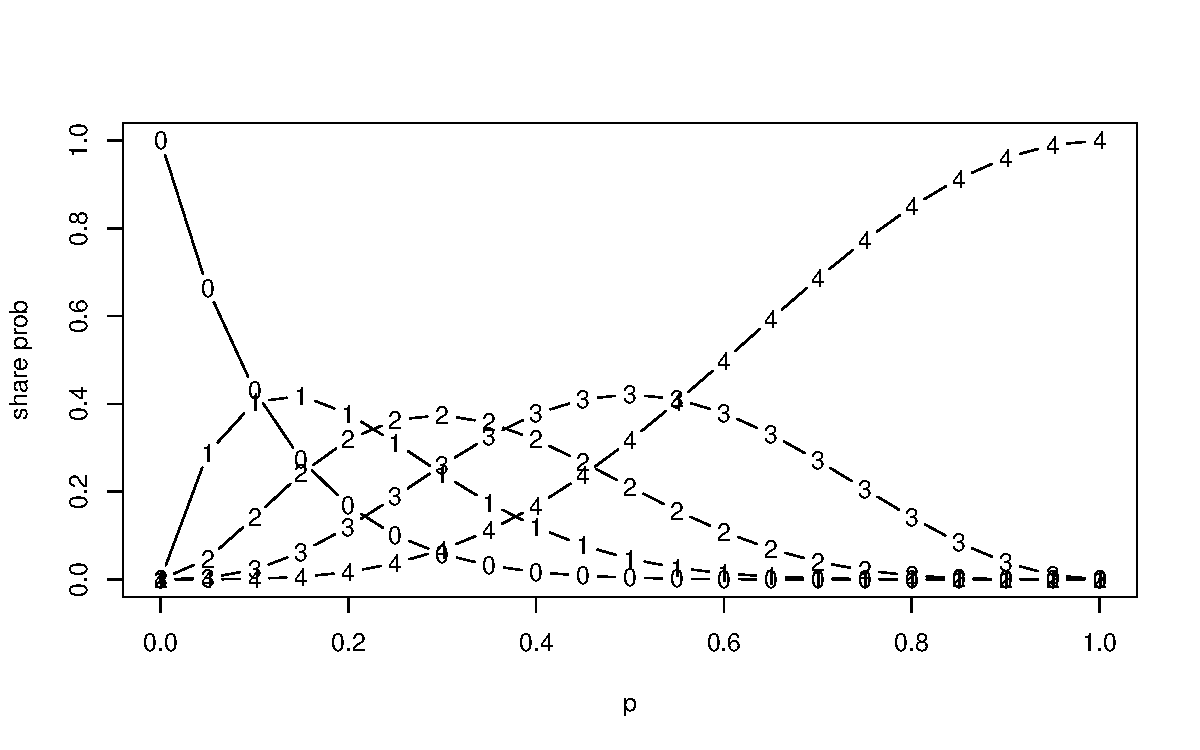
\includegraphics[width=\maxwidth]{/homes/gws/ruzzo/Documents/g/projects/thaps/Thaps_7_strains/code/snpNB/scripts/larrys/shared-snps/figs-knitr/share-plot-1} 

}

\caption[Sharing Probability]{Sharing Probability}\label{fig:share-plot}
\end{figure}


\end{knitrout}

\subsection{Old Tree Stuff}

All based on un-q-filtered reads.

The first pass at the tree analysis was the Chr1 tree, \emph{loose criteria} (c1); it is rendered via \\{\small\tt http://iubio.bio.indiana.edu/treeapp/treeprint-form.html} as Fig~\ref{fig:tree-v1}, and in newick format is:

%\noindent {\footnotesize\begin{verbatim}
%(((tp3367_Italy:4551,tp1013_Wales:4954):5920,(((tp1007_Virginia:10,tp1012_Australia:29):9,
%(tp1015_Puget_Sound:90,tp1335_NY:13):11):320,tp1014_Gyre:22):3484):8593);
%\end{verbatim}}
\begin{knitrout}\footnotesize
\definecolor{shadecolor}{rgb}{0.969, 0.969, 0.969}\color{fgcolor}\begin{kframe}
\begin{alltt}
\hlstd{newick.chr1.loose} \hlkwb{<-} \hlstr{'(((tp3367_Italy:4551,tp1013_Wales:4954):5920,(((tp1007_Virginia:10,tp1012_Australia:29):9,(tp1015_Puget_Sound:90,tp1335_NY:13):11):320,tp1014_Gyre:22):3484):8593,outgroup:0);'}
\hlkwd{cat.hardwrap}\hlstd{(newick.chr1.loose)}
\end{alltt}
\begin{verbatim}
# (((tp3367_Italy:4551,tp1013_Wales:4954):5920,(((tp1007_Virginia:10,tp1012_Austra 
# lia:29):9,(tp1015_Puget_Sound:90,tp1335_NY:13):11):320,tp1014_Gyre:22):3484):859 
# 3,outgroup:0);
\end{verbatim}
\end{kframe}
\end{knitrout}

\begin{figure}
  \begin{center}
    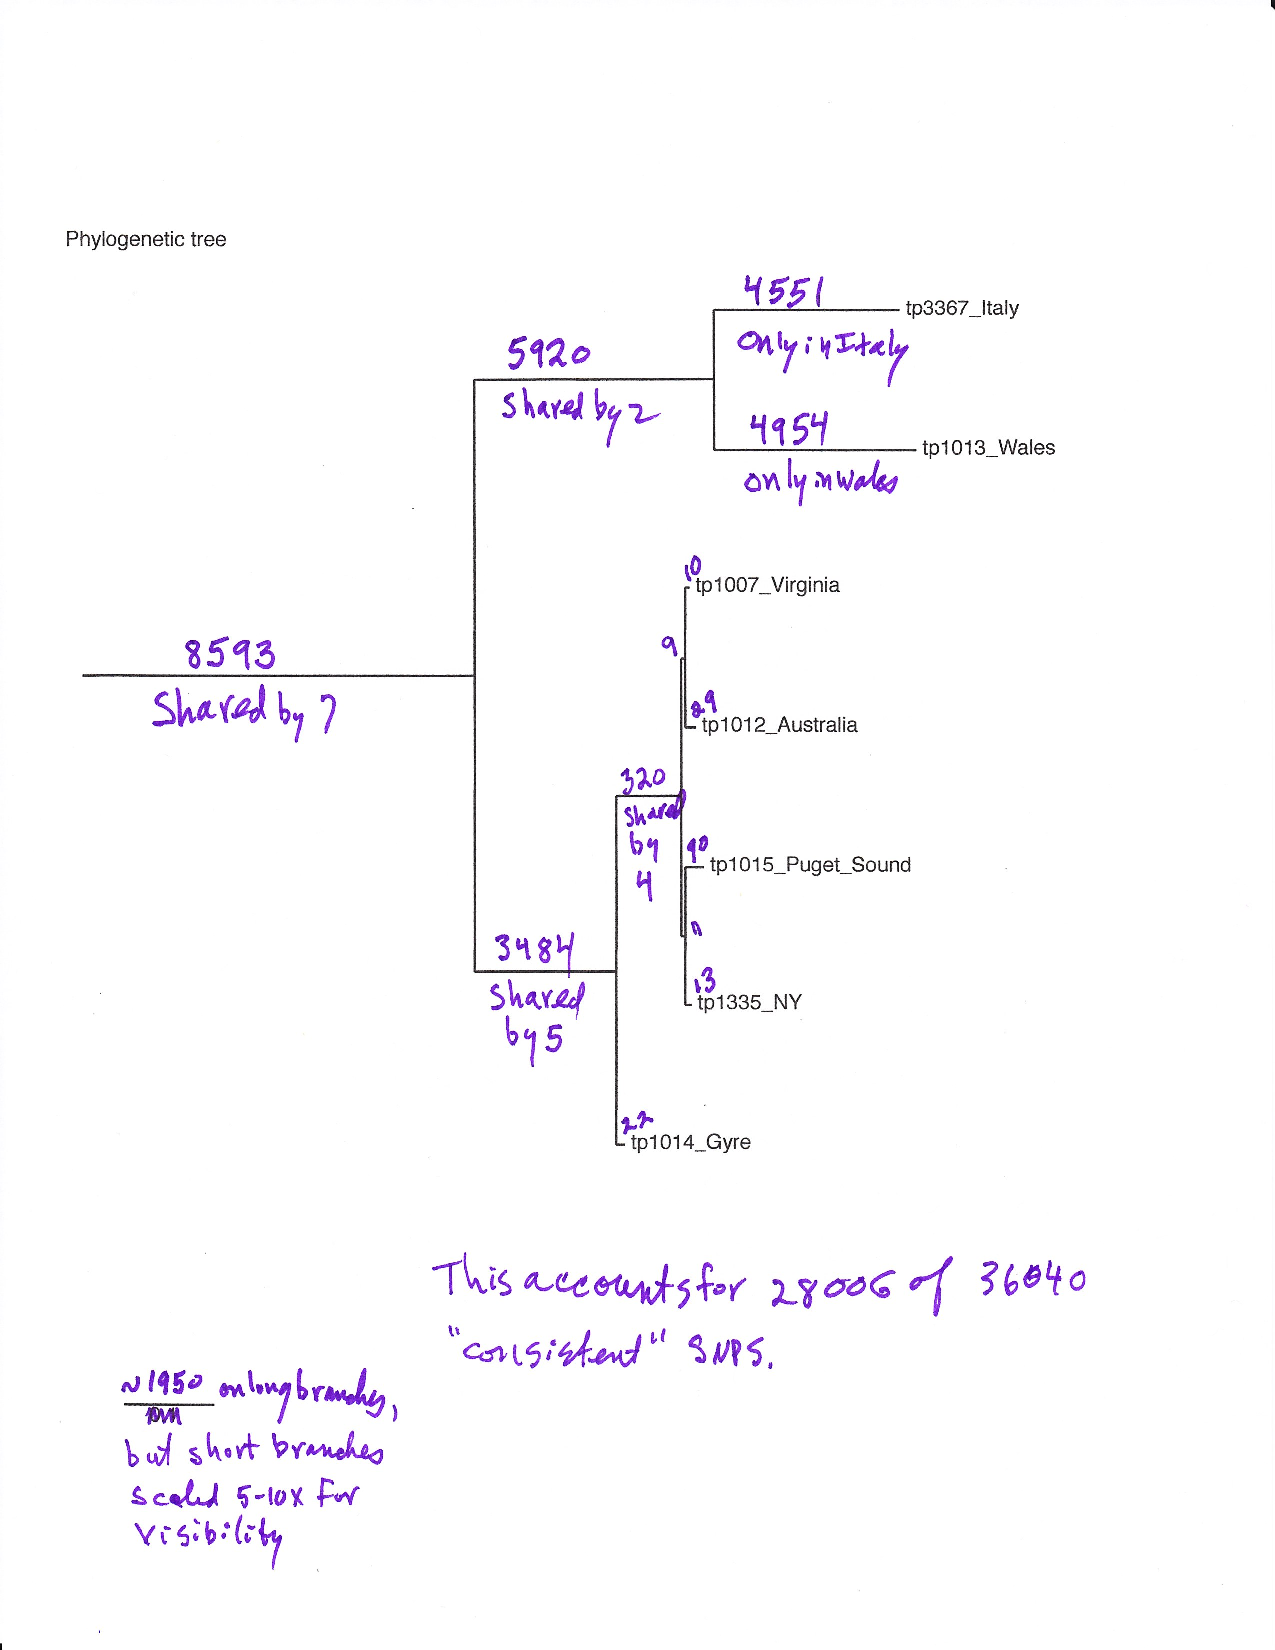
\includegraphics[scale=.5]{00old/shared-snp-tree-annotated-v1.pdf}
    \caption{Inferred Tree, based on Chr1, un-q-filtered reads, loose criteria.  (Note: to visually resolve the edges among the
      5, their lengths were scaled by 5x -- 10x in this figure, but not in the newick description
      shown in the text.)}
    \label{fig:tree-v1}
  \end{center}
\end{figure}

Chr 1 tree based on \emph{medium criteria} (c2) has exactly the same topology is, although the 
branch lengths are different.  As noted earlier, the length of the branch labeled ``*'' is probably
inflated by lower coverage and higher error rate in 1014, which may mask further legitimate sharing 
between it and the other L-isloates.  The branch lengths among the other 4 are too short for its 
topology to be convincing without a more rigorous analysis (e.g., a bootstrap test).

Chr1 tree, medium criteria, in newick format:

\begin{knitrout}\footnotesize
\definecolor{shadecolor}{rgb}{0.969, 0.969, 0.969}\color{fgcolor}\begin{kframe}
\begin{alltt}
\hlstd{newick.chr1.med} \hlkwb{<-} \hlstr{'(((tp3367_Italy:8813,tp1013_Wales:9652):9365,(((e_tp1007_Virginia:30,d_tp1012_Australia:61):19,(c_tp1015_Puget_Sound:207,b_tp1335_NY:41):18):1005,a_tp1014_Gyre:61):3912):7054,outgroup:0);'}
\hlkwd{cat.hardwrap}\hlstd{(newick.chr1.med)}
\end{alltt}
\begin{verbatim}
# (((tp3367_Italy:8813,tp1013_Wales:9652):9365,(((e_tp1007_Virginia:30,d_tp1012_Au 
# stralia:61):19,(c_tp1015_Puget_Sound:207,b_tp1335_NY:41):18):1005,a_tp1014_Gyre: 
# 61):3912):7054,outgroup:0);
\end{verbatim}
\end{kframe}
\end{knitrout}

NOTE: In early code, tree was not being recalculated; it was defined by constants in the following 
code chunk, hand-copied from the analysis above.  

\begin{knitrout}\scriptsize
\definecolor{shadecolor}{rgb}{0.969, 0.969, 0.969}\color{fgcolor}\begin{kframe}
\begin{alltt}
\hlcom{# tree parameters as nested lists }
\hlcom{#   Internal nodes have subtrees sub1/2 and length}
\hlcom{#   Root has sub1/2, but no length}
\hlcom{#   Leaves have where, length, optionally, id, alt, nb.  (Omit id for 'outgroup'. Use 'alt' for less formal}
\hlcom{#     labeling in cartoon version; it defaults to 'where'. Use 'nb' to add abcde annotations for legend.)}
\hlcom{# This hand-made version is now subsumed by make.tree; retained for comparison}
\hlstd{tree.by.hand} \hlkwb{<-}
  \hlkwd{list}\hlstd{(}
    \hlkwc{sub1} \hlstd{=} \hlkwd{list}\hlstd{(}
      \hlkwc{sub1} \hlstd{=} \hlkwd{list}\hlstd{(}
        \hlkwc{sub1} \hlstd{=} \hlkwd{list}\hlstd{(}\hlkwc{id}\hlstd{=}\hlnum{3367}\hlstd{,} \hlkwc{length}\hlstd{=}\hlnum{8813}\hlstd{,} \hlkwc{where}\hlstd{=}\hlstr{'Venice, Italy'}\hlstd{,} \hlkwc{alt}\hlstd{=}\hlstr{'Venice'}\hlstd{),}
        \hlkwc{sub2} \hlstd{=} \hlkwd{list}\hlstd{(}\hlkwc{id}\hlstd{=}\hlnum{1013}\hlstd{,} \hlkwc{length}\hlstd{=}\hlnum{9652}\hlstd{,} \hlkwc{where}\hlstd{=}\hlstr{'Wales, UK'}\hlstd{),}
        \hlkwc{length}\hlstd{=}\hlnum{9365}\hlstd{),}
      \hlkwc{sub2} \hlstd{=}  \hlkwd{list}\hlstd{(}
        \hlkwc{sub1} \hlstd{=} \hlkwd{list}\hlstd{(}
          \hlkwc{sub1} \hlstd{=} \hlkwd{list}\hlstd{(}
            \hlkwc{sub1} \hlstd{=} \hlkwd{list}\hlstd{(}\hlkwc{id}\hlstd{=}\hlnum{1007}\hlstd{,} \hlkwc{length}\hlstd{=}\hlnum{30}\hlstd{,} \hlkwc{nb}\hlstd{=}\hlstr{'e'}\hlstd{,} \hlkwc{where}\hlstd{=}\hlstr{'Virginia, USA'}\hlstd{),}
            \hlkwc{sub2} \hlstd{=} \hlkwd{list}\hlstd{(}\hlkwc{id}\hlstd{=}\hlnum{1012}\hlstd{,} \hlkwc{length}\hlstd{=}\hlnum{61}\hlstd{,} \hlkwc{nb}\hlstd{=}\hlstr{'d'}\hlstd{,} \hlkwc{where}\hlstd{=}\hlstr{'Perth, W. Australia'}\hlstd{,} \hlkwc{alt}\hlstd{=}\hlstr{'Perth'}\hlstd{),}
            \hlkwc{length}\hlstd{=}\hlnum{19}\hlstd{),}
          \hlkwc{sub2} \hlstd{=} \hlkwd{list}\hlstd{(}
            \hlkwc{sub1} \hlstd{=} \hlkwd{list}\hlstd{(}\hlkwc{id}\hlstd{=}\hlnum{1015}\hlstd{,} \hlkwc{length}\hlstd{=}\hlnum{207}\hlstd{,}\hlkwc{nb}\hlstd{=}\hlstr{'c'}\hlstd{,} \hlkwc{where}\hlstd{=}\hlstr{'Washington, USA'}\hlstd{,} \hlkwc{alt}\hlstd{=}\hlstr{'Puget Sound'}\hlstd{),}
            \hlkwc{sub2} \hlstd{=} \hlkwd{list}\hlstd{(}\hlkwc{id}\hlstd{=}\hlnum{1335}\hlstd{,} \hlkwc{length}\hlstd{=}\hlnum{41}\hlstd{,} \hlkwc{nb}\hlstd{=}\hlstr{'b'}\hlstd{,} \hlkwc{where}\hlstd{=}\hlstr{'New York, USA'}\hlstd{,}   \hlkwc{alt}\hlstd{=}\hlstr{'NY'}\hlstd{),}
            \hlkwc{length}\hlstd{=}\hlnum{18}\hlstd{),}
          \hlkwc{length}\hlstd{=}\hlnum{1005}\hlstd{),}
        \hlkwc{sub2} \hlstd{=} \hlkwd{list}\hlstd{(}\hlkwc{id}\hlstd{=}\hlnum{1014}\hlstd{,} \hlkwc{length}\hlstd{=}\hlnum{61}\hlstd{,} \hlkwc{nb}\hlstd{=}\hlstr{'a'}\hlstd{,} \hlkwc{where}\hlstd{=}\hlstr{'N. Pacific Gyre'}\hlstd{),}
        \hlkwc{length}\hlstd{=}\hlnum{3912}\hlstd{),}
      \hlkwc{length}\hlstd{=}\hlnum{7054}\hlstd{),}
    \hlkwc{sub2} \hlstd{=} \hlkwd{list}\hlstd{(}\hlkwc{length}\hlstd{=}\hlnum{0}\hlstd{,} \hlkwc{where}\hlstd{=}\hlstr{'outgroup'}\hlstd{)}
  \hlstd{)}

\hlcom{# historical, format example, and debug help:}
\hlstd{oldwick.medium} \hlkwb{<-} \hlstr{'(((CCMP3367_Italy:8813,CCMP1013_Wales:9652):9365,(((e_CCMP1007_Virginia:30,d_CCMP1012_Australia:61):19,(c_CCMP1015_Puget_Sound:207,b_CCMP1335_NY:41):18):1005,a_CCMP1014_NPG:61):3912):7054,outgroup:0);'}
\hlcom{# with simpler labeling for cartoon}
\hlstd{simple.oldwick.medium} \hlkwb{<-} \hlstr{'(((Italy:8813,Wales:9652):9365,(((Virginia:30,Australia:61):19,(Puget:207,NY:41):18):1005,Gyre:61):3912):7054,outgroup:0);'}
\hlkwd{cat.hardwrap}\hlstd{(oldwick.medium)}
\end{alltt}
\begin{verbatim}
# (((CCMP3367_Italy:8813,CCMP1013_Wales:9652):9365,(((e_CCMP1007_Virginia:30,d_CCM 
# P1012_Australia:61):19,(c_CCMP1015_Puget_Sound:207,b_CCMP1335_NY:41):18):1005,a_ 
# CCMP1014_NPG:61):3912):7054,outgroup:0);
\end{verbatim}
\begin{alltt}
\hlkwd{cat.hardwrap}\hlstd{(simple.oldwick.medium)}
\end{alltt}
\begin{verbatim}
# (((Italy:8813,Wales:9652):9365,(((Virginia:30,Australia:61):19,(Puget:207,NY:41) 
# :18):1005,Gyre:61):3912):7054,outgroup:0);
\end{verbatim}
\end{kframe}
\end{knitrout}

Two other versions of the tree, for possible use in figs in the main paper.

Figure~\ref{fig:tree-medium-unlabeled}:  [** as of 10/4/2015, this fig and next have stray stars on virginia, wales labels; probably due to hacking with commas in newick; not worth fixing unless we resurrect these trees for some purpose, but if so, see use of newick.name.undo in show.tree as probable fix. **]

\begin{knitrout}\scriptsize
\definecolor{shadecolor}{rgb}{0.969, 0.969, 0.969}\color{fgcolor}\begin{kframe}
\begin{alltt}
\hlstd{tree.scale} \hlkwb{<-} \hlkwd{ifelse}\hlstd{(}\hlkwd{which.snp.tables}\hlstd{(}\hlkwc{string.val}\hlstd{=F)[}\hlnum{1}\hlstd{]}\hlopt{==}\hlstr{'Chr1'}\hlstd{,} \hlnum{1}\hlstd{,} \hlnum{10}\hlstd{)}
\hlstd{tree.x.lim} \hlkwb{<-} \hlnum{3e4} \hlopt{*} \hlstd{tree.scale}
\hlstd{the.simple.tree} \hlkwb{<-} \hlkwd{read.tree}\hlstd{(}\hlkwc{text}\hlstd{=simple.newick.medium)}
\hlkwd{plot}\hlstd{(the.simple.tree,} \hlkwc{x.lim} \hlstd{= tree.x.lim)}
\hlkwd{axis}\hlstd{(}\hlnum{1}\hlstd{)}
\end{alltt}
\end{kframe}\begin{figure}

{\centering 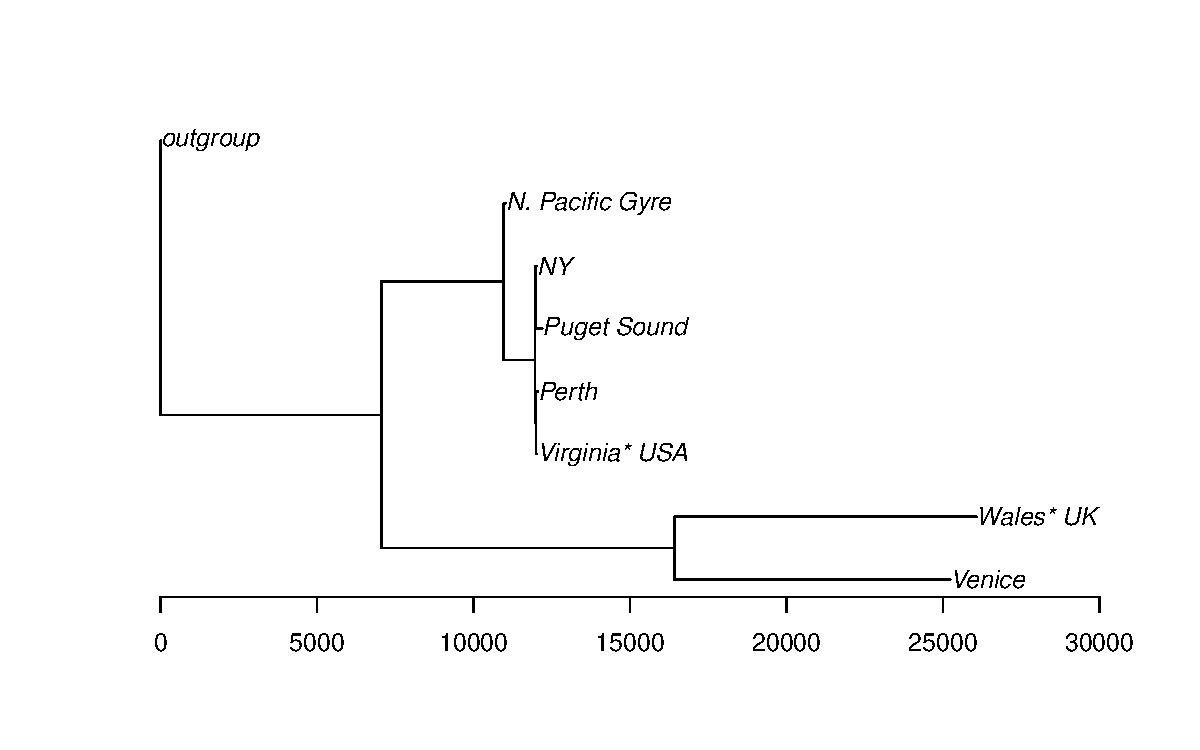
\includegraphics[width=3.5in]{/homes/gws/ruzzo/Documents/g/projects/thaps/Thaps_7_strains/code/snpNB/scripts/larrys/shared-snps/figs-knitr/newick-Chr1-unfiltered-tree-medium-unlabeled-1} 

}

\caption[Tree based on unfiltered reads and medium SNP filters]{Tree based on unfiltered reads and medium SNP filters.  ``Lengths'' are numbers of shared/private SNPs on Chr1. (no edge labels, nolegend)}\label{fig:tree-medium-unlabeled}
\end{figure}


\end{knitrout}

Figure~\ref{fig:tree-medium-unlabeled-shortscale}:

\begin{knitrout}\scriptsize
\definecolor{shadecolor}{rgb}{0.969, 0.969, 0.969}\color{fgcolor}\begin{kframe}
\begin{alltt}
\hlkwd{plot}\hlstd{(the.simple.tree,} \hlkwc{x.lim} \hlstd{= tree.x.lim)}
\hlkwd{axis}\hlstd{(}\hlnum{1}\hlstd{,(}\hlnum{0}\hlopt{:}\hlnum{4}\hlstd{)}\hlopt{*}\hlnum{7000}\hlopt{*}\hlstd{tree.scale,(}\hlnum{0}\hlopt{:}\hlnum{4}\hlstd{)}\hlopt{*}\hlnum{7000}\hlopt{*}\hlstd{tree.scale)}
\end{alltt}
\end{kframe}\begin{figure}

{\centering 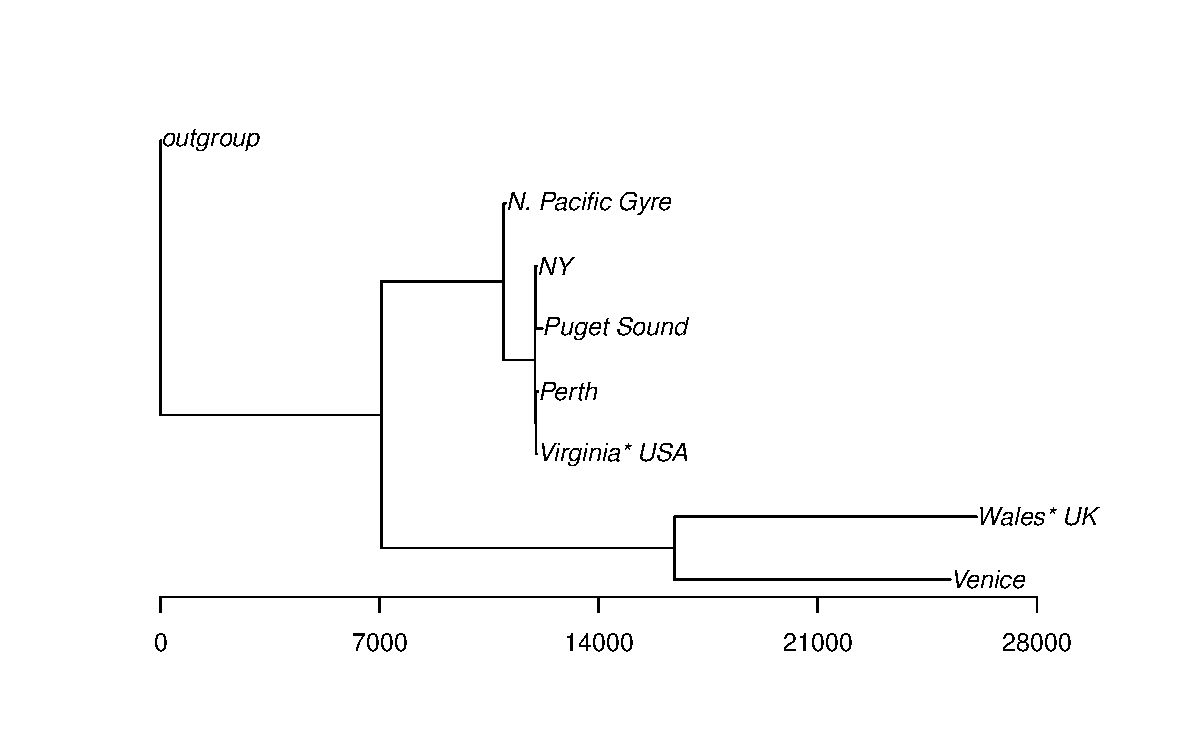
\includegraphics[width=3.5in]{/homes/gws/ruzzo/Documents/g/projects/thaps/Thaps_7_strains/code/snpNB/scripts/larrys/shared-snps/figs-knitr/newick-Chr1-unfiltered-tree-medium-unlabeled-shortscale-1} 

}

\caption[Tree based on unfiltered reads and medium SNP filters]{Tree based on unfiltered reads and medium SNP filters.  ``Lengths'' are numbers of shared/private SNPs on Chr1. (no edge labels, no legend, short scale bar)}\label{fig:tree-medium-unlabeled-shortscale}
\end{figure}


\end{knitrout}

At some much earlier point, Tony ran the whole-genome version of the then-current code above, and manually entered tree branch lengths/legend for the resuting tree, shown in Fig~\ref{fig:fullgenome-tree-medium}.  Code above can now automatically generate such a tree, but retain the following for comparison.  The basic story seems clear---same topology and branch lengths scaled by about 10x, which is completely reasonable given that Chr1 is about 10\% of the genome.  Note that this tree is not being recalculated; it is defined by constants in the following code chunk.

\begin{knitrout}\scriptsize
\definecolor{shadecolor}{rgb}{0.969, 0.969, 0.969}\color{fgcolor}\begin{kframe}
\begin{alltt}
\hlstd{fullgenome.newick.medium} \hlkwb{<-} \hlstr{'(((3367_Italy:86155,1013_Wales:95697):89598,(((e_1007_VA:330,d_1012_Australia:632):1296,(c_1015_WA:2113,b_1335_NY:658):480):10059,a_1014_NPG:568):39517):69526,outgroup:0);'}
\hlkwd{cat.hardwrap}\hlstd{(fullgenome.newick.medium)}
\end{alltt}
\begin{verbatim}
# (((3367_Italy:86155,1013_Wales:95697):89598,(((e_1007_VA:330,d_1012_Australia:63 
# 2):1296,(c_1015_WA:2113,b_1335_NY:658):480):10059,a_1014_NPG:568):39517):69526,o 
# utgroup:0);
\end{verbatim}
\begin{alltt}
\hlstd{legend.text} \hlkwb{<-} \hlkwd{c}\hlstd{(}\hlstr{'a: only in 1014  '}\hlstd{,}
                 \hlstr{'b: only in 1335  '}\hlstd{,}
                 \hlstr{'c: only in 1015  '}\hlstd{,}
                 \hlstr{'d: only in 1012  '}\hlstd{,}
                 \hlstr{'e: only in 1007  '}\hlstd{,}
                 \hlstr{'*: shared by bcde'}\hlstd{,}
                 \hlstr{'   shared by b/c '}\hlstd{,}
                 \hlstr{'   shared by d/e '}
\hlstd{)}
\hlstd{fullgenome.tree.x.lim} \hlkwb{<-} \hlnum{300000}
\hlstd{fullgenome.counts} \hlkwb{<-} \hlkwd{c}\hlstd{(} \hlnum{568}\hlstd{,} \hlnum{658}\hlstd{,} \hlnum{2113}\hlstd{,} \hlnum{632}\hlstd{,} \hlnum{330}\hlstd{,} \hlnum{10059}\hlstd{,} \hlnum{480}\hlstd{,} \hlnum{1296} \hlstd{)}
\hlstd{fullgenome.legend.text} \hlkwb{<-} \hlkwd{paste}\hlstd{(legend.text,}\hlkwd{format}\hlstd{(fullgenome.counts,}\hlkwc{width}\hlstd{=}\hlnum{5}\hlstd{),}\hlkwc{sep}\hlstd{=}\hlstr{' - '}\hlstd{)}
\hlstd{fullgenome.tree.labels} \hlkwb{<-} \hlkwd{list}\hlstd{(} \hlcom{## x,y,text}
     \hlnum{41000}\hlstd{,}\hlnum{3.63}\hlstd{,}\hlstr{'69526\textbackslash{}nshared by 7'}\hlstd{,}
     \hlnum{90000}\hlstd{,}\hlnum{5.75}\hlstd{,}\hlstr{'39517\textbackslash{}nby 5 (**)'}\hlstd{,}
    \hlnum{115000}\hlstd{,}\hlnum{1.5}\hlstd{,} \hlstr{'89598\textbackslash{}nshared by 2'}\hlstd{,}
    \hlnum{210000}\hlstd{,}\hlnum{2.0}\hlstd{,} \hlstr{'95697 only\textbackslash{}nin Wales'}\hlstd{,}
    \hlnum{210000}\hlstd{,}\hlnum{1.0}\hlstd{,} \hlstr{'86155 only\textbackslash{}nin Italy'}\hlstd{,}
    \hlnum{113500}\hlstd{,}\hlnum{4.6}\hlstd{,} \hlstr{'*'}\hlstd{)}
\end{alltt}
\end{kframe}
\end{knitrout}

Figure~\ref{fig:fullgenome-tree-medium}:

\begin{knitrout}\scriptsize
\definecolor{shadecolor}{rgb}{0.969, 0.969, 0.969}\color{fgcolor}\begin{kframe}
\begin{alltt}
\hlkwd{library}\hlstd{(ape)}
\hlstd{the.fullgenome.tree} \hlkwb{<-} \hlkwd{read.tree}\hlstd{(}\hlkwc{text}\hlstd{=fullgenome.newick.medium)}
\hlkwd{plot}\hlstd{(the.fullgenome.tree,} \hlkwc{x.lim} \hlstd{= fullgenome.tree.x.lim)}
\hlkwd{axis}\hlstd{(}\hlnum{1}\hlstd{)} \hlcom{# ; axis(2) useful only for placing labels}
\hlstd{opar} \hlkwb{<-} \hlkwd{par}\hlstd{(}\hlkwc{family}\hlstd{=}\hlstr{'mono'}\hlstd{,}\hlkwc{cex}\hlstd{=}\hlnum{.8}\hlstd{)}
\hlkwd{legend}\hlstd{(}\hlstr{'topright'}\hlstd{,} \hlkwc{legend}\hlstd{=fullgenome.legend.text)}
\hlkwd{par}\hlstd{(opar)}
\hlkwa{for}\hlstd{(i} \hlkwa{in} \hlkwd{seq}\hlstd{(}\hlnum{1}\hlstd{,}\hlkwd{length}\hlstd{(fullgenome.tree.labels)}\hlopt{-}\hlnum{2}\hlstd{,}\hlkwc{by}\hlstd{=}\hlnum{3}\hlstd{))\{}
  \hlkwd{text}\hlstd{(fullgenome.tree.labels[[i]], fullgenome.tree.labels[[i}\hlopt{+}\hlnum{1}\hlstd{]], fullgenome.tree.labels[[i}\hlopt{+}\hlnum{2}\hlstd{]])}
\hlstd{\}}
\end{alltt}
\end{kframe}\begin{figure}

{\centering 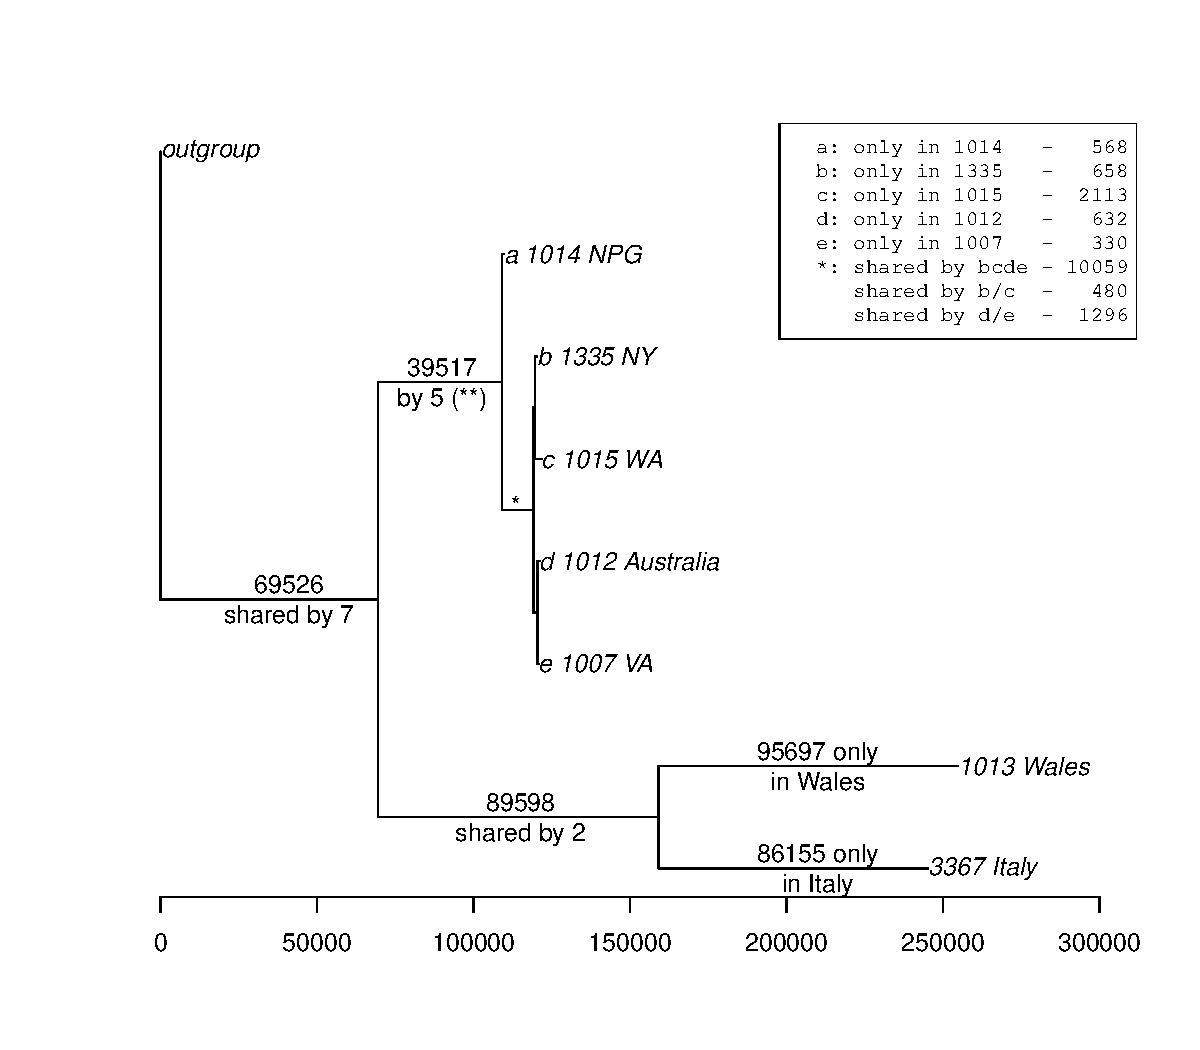
\includegraphics[width=\maxwidth]{/homes/gws/ruzzo/Documents/g/projects/thaps/Thaps_7_strains/code/snpNB/scripts/larrys/shared-snps/figs-knitr/fullgenome-tree-medium-1} 

}

\caption[Tree based on unqfiltered reads and medium SNP filters]{Tree based on unqfiltered reads and medium SNP filters.  ``Lengths'' are numbers of shared/private SNPs genome-wide. (By-hand legacy version)}\label{fig:fullgenome-tree-medium}
\end{figure}


\end{knitrout}

\FloatBarrier

% remember to do this to enable Id keyword substution: svn propset svn:keywords Id shared-snps.rnw 
\mbox{}\vfill\footnotesize\flushright SVN, ID I miss you.\ $ $Id: shared-snps.rnw  2017-06-29 or later. ruzzo $ $
\end{document}
